% !TeX encoding = UTF-8
% !TeX program = xelatex
% !TeX spellcheck = en_US

\documentclass[degree=doctor,language=chinese,cjk-font=external]{sustechthesis}
  % 学位 degree:
  %   master (默认) | doctor
  % 语言 language:
  %   chinese (默认)| english
  % 中文字体 cjk-font
  %   auto (默认,自动选择系统自带字体)| external (包内字体)| windows | mac | 等
  %   在 **非Windows** 的系统上推荐使用包内字体,而非系统字体。
  %   以达到和 Windows 系统上显示的字体效果。
  %   Windows 系统上可以删除该参数,使用系统内置字体。


\newcommand{\lei}[1]{{\leavevmode\color{blue}#1}}
\newcommand{\leir}[1]{{\leavevmode\color{red}#1}}

\usepackage
[
bookmarks=true,
pdfborder={0 0 0},
linktocpage,
breaklinks=true,
colorlinks,
citecolor=blue,
filecolor=black,
linkcolor=red,
urlcolor=red
pdftex
]{hyperref}

\usepackage{subfigure}
\usepackage{longtable}

% 论文基本配置,加载宏包等全局配置
% 在此文件中可以选择
% 1. 生成的PDF为无空白页的用于电子版提交的版本 或 插入空白页的以便双面打印的版本
% 2. 学位学科门类(理学、工学、医学)
% 3. 培养单位
% 4. 作者姓名、指导教师等
% 5. 修改gongshuo的值, 默认为false代表生成学术型研究生毕业设计模板, 改为true则将生成专业型研究生毕业设计模板
%% !TeX root = ./sustechthesis-example.tex

% 论文基本信息配置

\thusetup{
  %******************************
  % 注意:
  %   1. 配置里面不要出现**空行**
  %   2. 不需要的配置信息可以删除
  %   3. 建议先阅读文档中所有关于选项的说明
  %******************************
  %
  % 输出格式
  %   选择打印版(print)或用于提交的电子版(electronic),前者会插入空白页以便直接双面打印
  %
  output = electronic,
  %
  % 标题
  %   可使用“\\”命令手动控制换行
  %   如果需要使用副标题,取消 subtitle 和 subtitle* 的注释即可。
  %
  title  = {南方科技大学学位论文 \LaTeX{} 模板 (Support English) 使用示例文档 v\version},
  title* = {An Introduction to \LaTeX{} Thesis Template of Southern University of Science and Technology v\version},
  % subtitle = {可选的副标题可选的副标题可选的副标题可选的副标题可选的副标题可选的副标题},
  % subtitle* = {optional subtitle optional subtitle optional subtitle optional subtitle optional subtitle optional subtitle},
  %
  % 学位
  %
  degree-domain = {工学}, % 【中文】学科门类:可选理学、工学、医学
  degree-domain* = {Engineering}, % 【英文】学位等级:可选Science, Engineering, Medicine
  gongshuo = false, % 是否为专业型学位。专业型学位则填 true ,学术型或其他为 false 。
  %
  % 培养单位
  %   填写所属院系的全名
  %   超长英文系名可以手动换行
  department = {计算机科学与工程系},
  department* = {School of System Design and \\Intelligent Manufacturing},
  %
  % 学科
  %   1. 学术型学位
  %      获得一级学科授权的学科填写一级学科名称,其他填写二级学科名称
  %   2. 工程硕士
  %      工程领域名称
  %
  discipline  = {计算机科学与技术},
  discipline* = {Computer Science and Technology},
  %
  % 姓名
  %   英文用全拼,姓在前,名在后,姓和名的首字母大写,其余小写
  %
  author  = {李子强},
  author* = {Li Ziqiang},
  %
  % 指导教师
  %   中文姓名和职称之间以英文逗号“,”分开,下同
  %
  supervisor  = {某某某(Alice Bob)助理教授},
  supervisor* = {Assistant Professor Alice Bob},
  %
  % 日期
  %   使用 ISO 格式;默认为当前时间
  %   date 为第一页全中文大写日期,defense-date 为第二、三页的答辩日期。
  %   需要按 {年-月-日} 格式填写,如不显示“日”,可以随意填一个日期,但是不能为空。
  %
  date = {2020-12-20},
  defense-date = {2020-12-20},
  %
  % 密级
  %   公开, 秘密, 机密, 绝密
  %
  statesecrets={公开},
  %
  % 国内图书分类号,国际图书分类号
  %
  natclassifiedindex={TM301.2},
  intclassifiedindex={62-5},
}

% 载入所需的宏包

% 可以使用 nomencl 生成符号和缩略语说明
% \usepackage{nomencl}
% \makenomenclature

% 表格加脚注
\usepackage{threeparttable}

% 表格中支持跨行
\usepackage{multirow}

% 量和单位
\usepackage{siunitx}

% 定理类环境宏包
\usepackage{amsthm}
% 也可以使用 ntheorem
% \usepackage[amsmath,thmmarks,hyperref]{ntheorem}

%%%%%% 参考文献编译方式二选一,不要同时开启。
%%%% 选择一
%% 参考文献使用 BibTeX + natbib 宏包
%% 顺序编码制
\usepackage[sort&compress]{gbt7714}
\bibliographystyle{gbt7714-numerical}
\usepackage{bibunits}

%%%% 选择二(不兼容本模板,请勿使用)
%% 参考文献使用 BibLaTeX 宏包
% \usepackage[backend=biber,style=gb7714-2015]{biblatex}
%% 声明 BibLaTeX 的数据库
% \addbibresource{ref/refs.bib}

% 定义所有的图片文件在 figures 子目录下
\graphicspath{{figures/}}

% 数学命令
\newcommand\dif{\mathop{}\!\mathrm{d}}  % 微分符号

% hyperref 宏包在最后调用
\usepackage{hyperref}
\usepackage{ragged2e}

% 固定宽度的表格。放在 hyperref 之前的话,tabularx 里的 footnote 显示不出来。
\usepackage{tabularx}

% 跨页表格,必须在 hyperref 之后使用否则会报错。
\usepackage{longtable}


\begin{document}

%\nobibliography*
%\newgeometry{top=1in,bottom=0in,right=0in,left=0in}
% !TeX spellcheck = en_US

\thispagestyle{empty}

\begin{center}

%	\pagecolor{Dandelion}
	
%	\begin{flushleft}
%		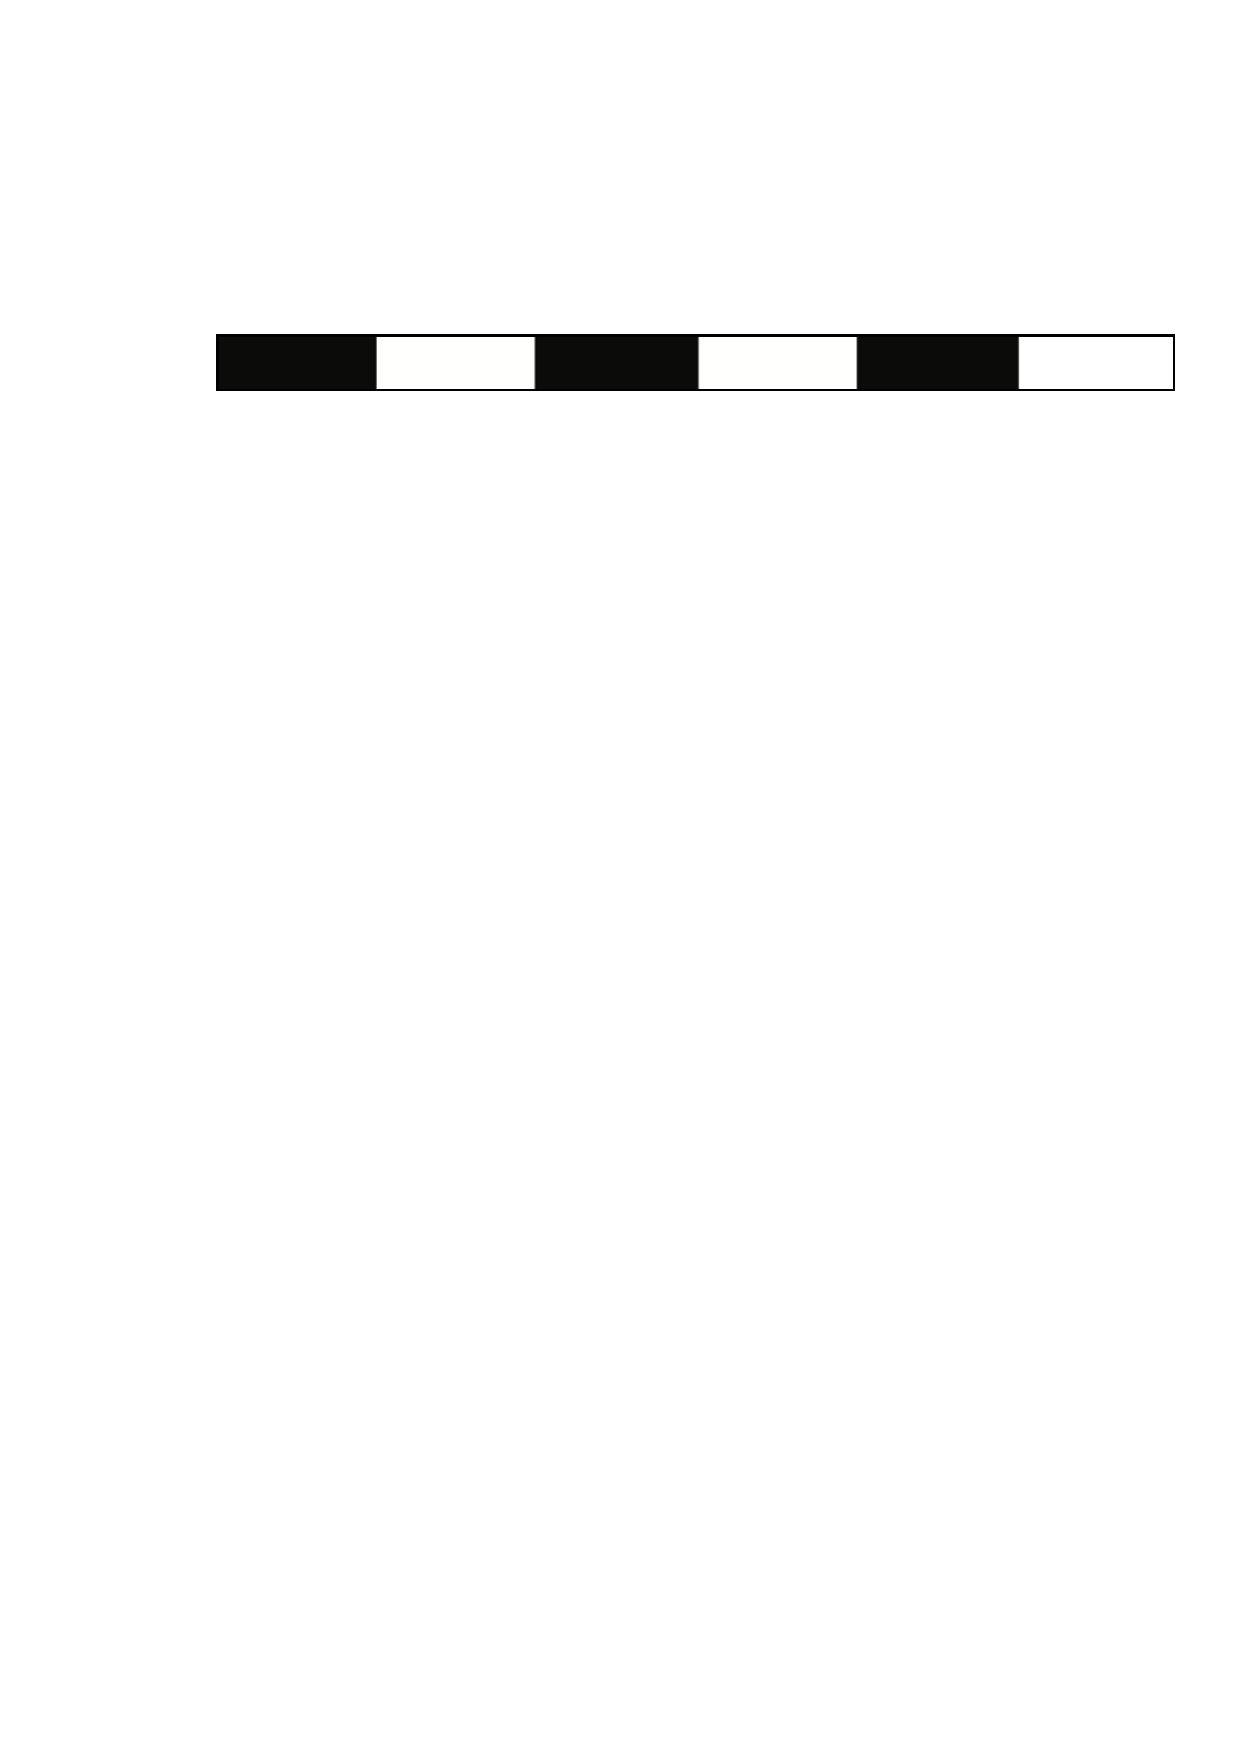
\includegraphics[scale=1.29]{JasonFrontCover.pdf}
%		%\includegraphics[scale=1.15]{Frontpage_Kn.pdf}
%	\end{flushleft}


	\vspace{1cm}
	\LARGE
	\textbf{稀薄气体动力学}
	
%	\vspace{1.5cm}
%	%\hskip 4cm
%	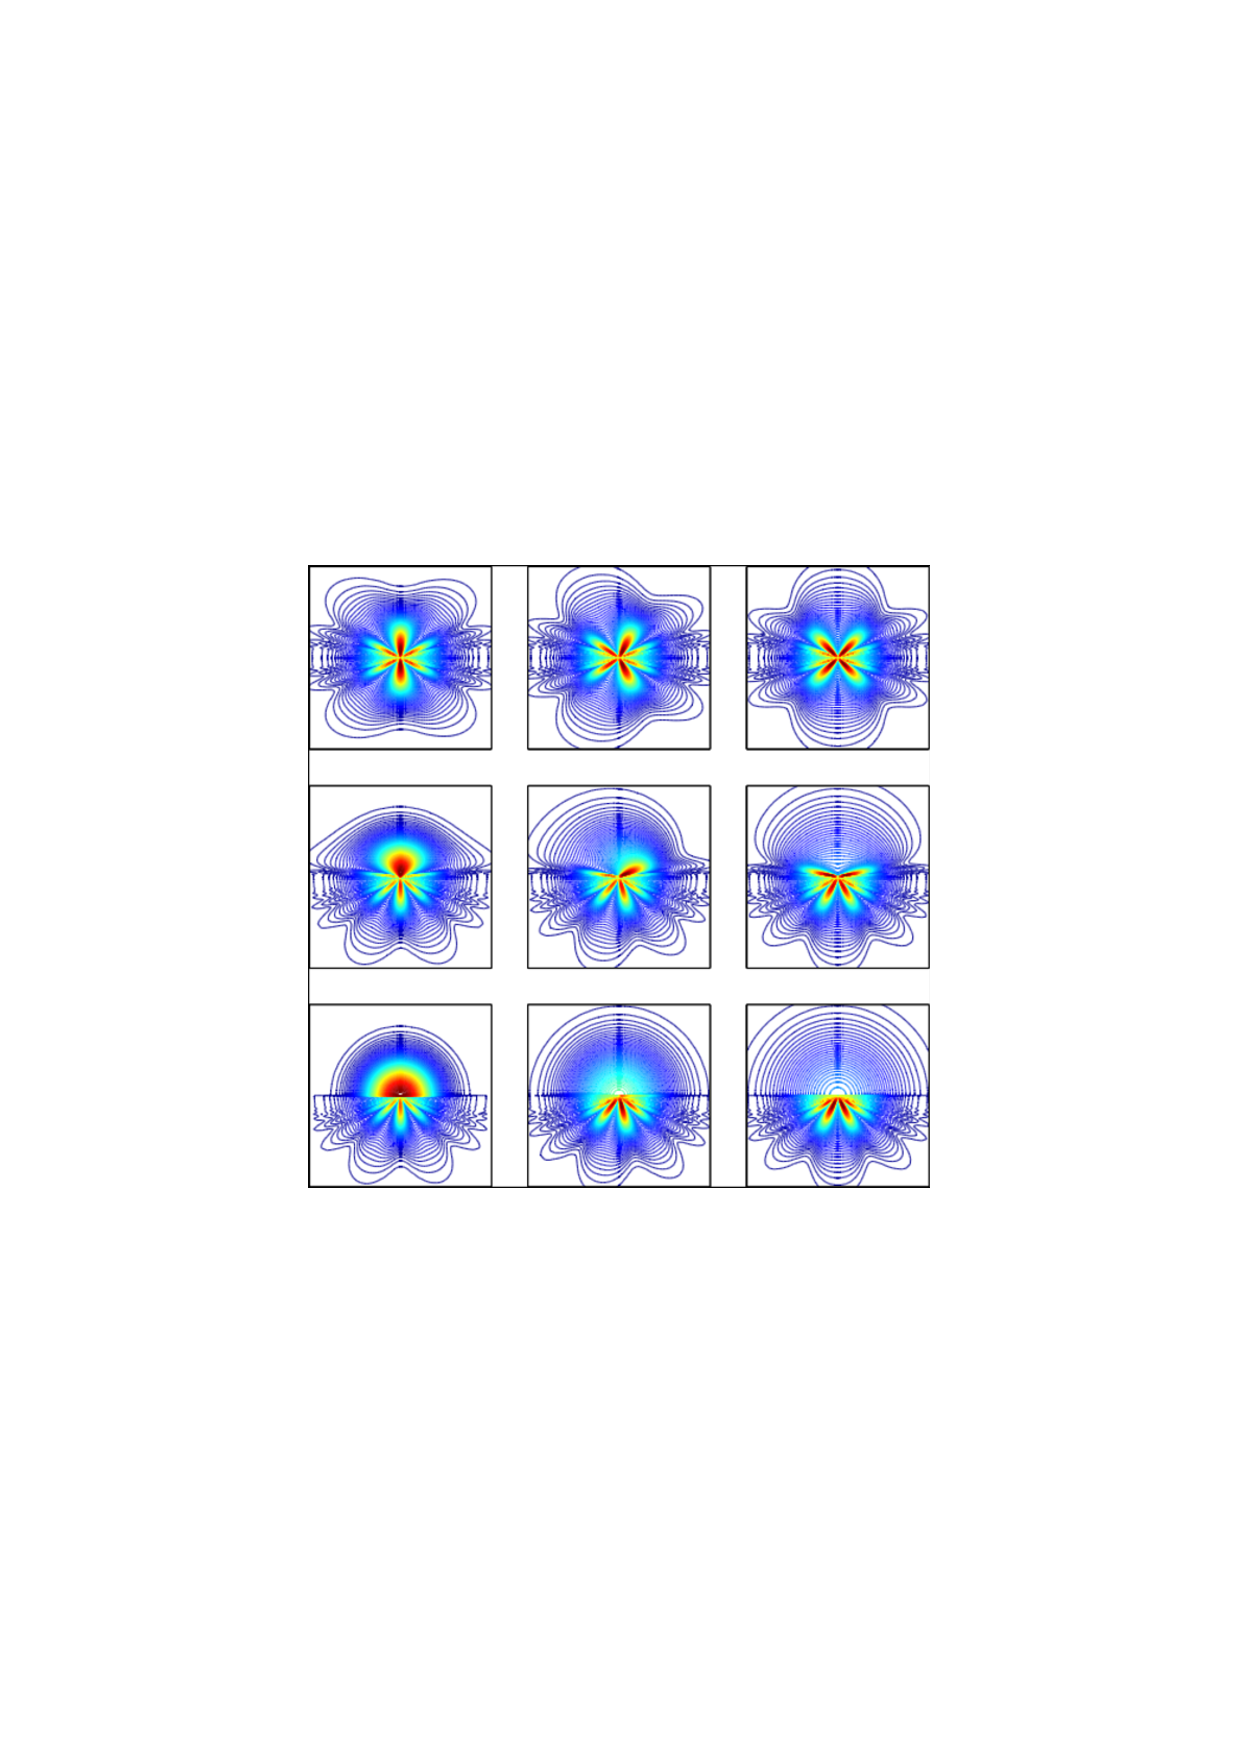
\includegraphics[scale=1]{FrontPage2.pdf}
	
	
	\vspace{2.5cm}
	\Large
	\textbf{吴雷 ~ 李琪 ~ 编著 }
	
%	\Large
%%	Department of Mechanics and Aerospace Engineering\\
%	Southern University of Science and Technology
	
% 2021/12
	
\end{center}



%%%%%%%%%%%%
%\pagebreak
%\pagecolor{white}

% 封面
%\maketitle

% 学位论文公开评阅人和答辩委员会名单
%% !TeX root = ../sustechthesis-example.tex




% 南方科技大学学位论文原创性声明和使用授权说明
% 本模版不会对扫描版的页码进行处理,建议定稿后打印声明页再插入编译,以免页码出错。
% 或者,使用其他 pdf 拼接软件也可达到替换声明页面的目的。
%\statementcopyright % 生成未签名的声明
% \statementcopyright[scan-statement.pdf] % 插入已签名的声明文件(扫描版)

%\frontmatter
%% !TeX root = ../sustechthesis-example.tex

% 中英文摘要和关键字

\begin{abstract}
  论文的摘要是对论文研究内容和成果的高度概括。
  摘要应对论文所研究的问题及其研究目的进行描述,对研究方法和过程进行简单介绍,对研究成果和所得结论进行概括。
  摘要应具有独立性和自明性,其内容应包含与论文全文同等量的主要信息。
  使读者即使不阅读全文,通过摘要就能了解论文的总体内容和主要成果。

  论文摘要的书写应力求精确、简明。
  切忌写成对论文书写内容进行提要的形式,尤其要避免“第 1 章……;第 2 章……;……”这种或类似的陈述方式。
  
  博士论文摘要约 800~1000 字,硕士论文摘要的字数一般为 500 字左右,且篇幅限制在一页内书写。

  关键词是为了文献标引工作、用以表示全文主要内容信息的单词或术语。
  关键词不超过 5 个,每个关键词中间用分号分隔。

  % 关键词用“英文逗号”分隔,输出时会自动处理为正确的分隔符
  \thusetup{
    keywords = {关键词 1, 关键词 2, 关键词 3, 关键词 4, 长长长长长长长长长长长长长长长长长长长长长长长长长关键词 5},
  }
\end{abstract}

\begin{abstract*}
  An abstract of a dissertation is a summary and extraction of research work and contributions.
  Included in an abstract should be description of research topic and research objective, brief introduction to methodology and research process, and summarization of conclusion and contributions of the research.
  An abstract should be characterized by independence and clarity and carry identical information with the dissertation.
  It should be such that the general idea and major contributions of the dissertation are conveyed without reading the dissertation.

  An abstract should be concise and to the point.
  It is a misunderstanding to make an abstract an outline of the dissertation and words “the first chapter”, “the second chapter” and the like should be avoided in the abstract.

  The abstract of the doctoral thesis is about 800 to 1000 words; the abstract of the master's thesis is generally about 500 words; the length is limited to one page.

  Keywords are terms used in a dissertation for indexing, reflecting core information of the dissertation.
  An abstract may contain a maximum of 5 keywords, with semi-colons used in between to separate one another.

  % Use comma as seperator when inputting
  \thusetup{
    keywords* = {keyword 1, keyword 2, keyword 3, keyword 4, looooooooooooooooooooong keyword 5},
  }
\end{abstract*}


% 目录
\tableofcontents

% 插图和附表清单
% \listoffiguresandtables  % 插图和附表清单
% \listoffigures           % 插图清单
% \listoftables            % 附表清单

% 符号对照表(非强制性要求,如果论文中所用符号不多,可以略去)
%% !TeX root = ../sustechthesis-example.tex

% denotation 环境带一个可选参数,用来指定符号列的宽度(默认为 2.5cm),下面改3cm为例。
\begin{denotation}[3cm]
  \item[PI] 聚酰亚胺
  \item[MPI] 聚酰亚胺模型化合物,N-苯基邻苯酰亚胺
  \item[PBI] 聚苯并咪唑
  \item[MPBI] 聚苯并咪唑模型化合物,N-苯基苯并咪唑
  \item[PY] 聚吡咙
  \item[PMDA-BDA] 均苯四酸二酐与联苯四胺合成的聚吡咙薄膜
  \item[MPY] 聚吡咙模型化合物
  \item[As-PPT] 聚苯基不对称三嗪
  \item[MAsPPT] 聚苯基不对称三嗪单模型化合物,3,5,6-三苯基-1,2,4-三嗪
  \item[DMAsPPT] 聚苯基不对称三嗪双模型化合物(水解实验模型化合物)
  \item[S-PPT] 聚苯基对称三嗪
  \item[MSPPT] 聚苯基对称三嗪模型化合物,2,4,6-三苯基-1,3,5-三嗪
  \item[PPQ] 聚苯基喹噁啉
  \item[MPPQ] 聚苯基喹噁啉模型化合物,3,4-二苯基苯并二嗪
  \item[HMPI] 聚酰亚胺模型化合物的质子化产物
  \item[HMPY] 聚吡咙模型化合物的质子化产物
  \item[HMPBI] 聚苯并咪唑模型化合物的质子化产物
  \item[HMAsPPT] 聚苯基不对称三嗪模型化合物的质子化产物
  \item[HMSPPT] 聚苯基对称三嗪模型化合物的质子化产物
  \item[HMPPQ] 聚苯基喹噁啉模型化合物的质子化产物
  \item[PDT] 热分解温度
  \item[HPLC] 高效液相色谱 (High Performance Liquid Chromatography)
  \item[HPCE] 高效毛细管电泳色谱 (High Performance Capillary lectrophoresis)
  \item[LC-MS] 液相色谱-质谱联用 (Liquid chromatography-Mass Spectrum)
  \item[TIC] 总离子浓度 (Total Ion Content)
  \item[\textit{ab initio}] 基于第一原理的量子化学计算方法,常称从头算法
  \item[DFT] 密度泛函理论 (Density Functional Theory)
  \item[$E_a$] 化学反应的活化能 (Activation Energy)
  \item[ZPE] 零点振动能 (Zero Vibration Energy)
  \item[PES] 势能面 (Potential Energy Surface)
  \item[TS] 过渡态 (Transition State)
  \item[TST] 过渡态理论 (Transition State Theory)
  \item[$\increment G^\neq$] 活化自由能(Activation Free Energy)
  \item[$\kappa$] 传输系数 (Transmission Coefficient)
  \item[IRC] 内禀反应坐标 (Intrinsic Reaction Coordinates)
  \item[$\nu_i$] 虚频 (Imaginary Frequency)
  \item[ONIOM] 分层算法 (Our own N-layered Integrated molecular Orbital and molecular Mechanics)
  \item[SCF] 自洽场 (Self-Consistent Field)
  \item[SCRF] 自洽反应场 (Self-Consistent Reaction Field)
\end{denotation}



% 也可以使用 nomencl 宏包,需要在导言区
% \usepackage{nomencl}
% \makenomenclature

% 在这里输出符号说明
% \printnomenclature[3cm]

% 在正文中的任意为都可以标题
% \nomenclature{PI}{聚酰亚胺}
% \nomenclature{MPI}{聚酰亚胺模型化合物,N-苯基邻苯酰亚胺}
% \nomenclature{PBI}{聚苯并咪唑}
% \nomenclature{MPBI}{聚苯并咪唑模型化合物,N-苯基苯并咪唑}
% \nomenclature{PY}{聚吡咙}
% \nomenclature{PMDA-BDA}{均苯四酸二酐与联苯四胺合成的聚吡咙薄膜}
% \nomenclature{MPY}{聚吡咙模型化合物}
% \nomenclature{As-PPT}{聚苯基不对称三嗪}
% \nomenclature{MAsPPT}{聚苯基不对称三嗪单模型化合物,3,5,6-三苯基-1,2,4-三嗪}
% \nomenclature{DMAsPPT}{聚苯基不对称三嗪双模型化合物(水解实验模型化合物)}
% \nomenclature{S-PPT}{聚苯基对称三嗪}
% \nomenclature{MSPPT}{聚苯基对称三嗪模型化合物,2,4,6-三苯基-1,3,5-三嗪}
% \nomenclature{PPQ}{聚苯基喹噁啉}
% \nomenclature{MPPQ}{聚苯基喹噁啉模型化合物,3,4-二苯基苯并二嗪}
% \nomenclature{HMPI}{聚酰亚胺模型化合物的质子化产物}
% \nomenclature{HMPY}{聚吡咙模型化合物的质子化产物}
% \nomenclature{HMPBI}{聚苯并咪唑模型化合物的质子化产物}
% \nomenclature{HMAsPPT}{聚苯基不对称三嗪模型化合物的质子化产物}
% \nomenclature{HMSPPT}{聚苯基对称三嗪模型化合物的质子化产物}
% \nomenclature{HMPPQ}{聚苯基喹噁啉模型化合物的质子化产物}
% \nomenclature{PDT}{热分解温度}
% \nomenclature{HPLC}{高效液相色谱 (High Performance Liquid Chromatography)}
% \nomenclature{HPCE}{高效毛细管电泳色谱 (High Performance Capillary lectrophoresis)}
% \nomenclature{LC-MS}{液相色谱-质谱联用 (Liquid chromatography-Mass Spectrum)}
% \nomenclature{TIC}{总离子浓度 (Total Ion Content)}
% \nomenclature{\textit{ab initio}}{基于第一原理的量子化学计算方法,常称从头算法}
% \nomenclature{DFT}{密度泛函理论 (Density Functional Theory)}
% \nomenclature{$E_a$}{化学反应的活化能 (Activation Energy)}
% \nomenclature{ZPE}{零点振动能 (Zero Vibration Energy)}
% \nomenclature{PES}{势能面 (Potential Energy Surface)}
% \nomenclature{TS}{过渡态 (Transition State)}
% \nomenclature{TST}{过渡态理论 (Transition State Theory)}
% \nomenclature{$\increment G^\neq$}{活化自由能(Activation Free Energy)}
% \nomenclature{$\kappa$}{传输系数 (Transmission Coefficient)}
% \nomenclature{IRC}{内禀反应坐标 (Intrinsic Reaction Coordinates)}
% \nomenclature{$\nu_i$}{虚频 (Imaginary Frequency)}
% \nomenclature{ONIOM}{分层算法 (Our own N-layered Integrated molecular Orbital and molecular Mechanics)}
% \nomenclature{SCF}{自洽场 (Self-Consistent Field)}
% \nomenclature{SCRF}{自洽反应场 (Self-Consistent Reaction Field)}



% 正文部分
\mainmatter

\input{Introduction/Introduction}
% !TeX root = ../sustechthesis-example.tex

\chapter{气体动理论}


\section{理想气体}


\section{速度分布函数与宏观量}\label{sec:Boltzmann}

在气体动理论中,单原子气体在相空间中的概率密度由速度分布函数$f(t,\bm{x},\bm{v})$表示,是时间$t$, 空间坐标$ \bm{x}=(x_1,x_2,x_3)$ 和 分子速度$\bm{v}=(v_1,v_2,v_3)$的函数. 定义$f(t,\bm{x},\bm{v})d\bm{x}d\bm{v}$是体积为$d\bm{x}d\bm{v}$的相空间上的分子数,则气体的数密度$n$、宏观速度$\bm{u}$、温度$T$、压力张量$p_{ij}$和热流$\bm{q}$可以分别通过对速度分布函数求矩得到:
\begin{equation}\label{macroscopic_origin}
\begin{aligned}[b]
&n(t,\bm{x})=\int{}f(t,\bm{x},\bm{v})d\bm{v}, \\  &\bm{u}(t,\bm{x})=\frac{1}{n(t,\bm{x})}\int\bm{v}f(t,\bm{x},\bm{v})d\bm{v},\\   &T(t,\bm{x})=\frac{m}{3k_Bn(t,\bm{x})}\int{}c^2f(t,\bm{x},\bm{v})d\bm{v}, \\    &p_{ij}(t,\bm{x})={}m\int{}c_ic_jf(t,\bm{x},\bm{v})d\bm{v}, \\  &\bm{q}(t,\bm{x})=\frac{m}{2}\int{}c^2\bm{c}f(t,\bm{x},\bm{v})d\bm{v},
\end{aligned}
\end{equation}
其中, $\bm{c}=\bm{v}-\bm{u}$是气体分子热运动速度, 即气体分子速度与当地宏观速度的矢量差,而$c$是热运动速率. 定义应力偏量为
\begin{equation}
\sigma_{ij}=p_{ij}-p\delta_{ij},
\end{equation}
其中$p=nk_BT$, $\delta_{ij}$为克罗内克函数. 


\section{Boltzmann方程}

The governing equation for the evolution of VDF of a dilute gas system is derived by Ludwig Boltzmann. In his description, molecules move in straight lines with fixed velocities until they encounter elastic collisions with other molecules. This is justified by the fact that, at standard temperature and pressure, the MFP of gas molecules is hundreds times of the nominal atomic diameter and about 30 times the average molecular separation.  

Both molecular streaming and collision change the VDF in the phase space as per the Boltzmann equation~\cite{CE,Cercignani1990,henning,Kremer2009book}:
\begin{equation}\label{Boltzmann}
\frac{\partial f}{\partial t}+\bm{v}\cdot\frac{\partial f}{\partial
	\bm{x}}+\bm{a}\cdot\frac{\partial f}{\partial \bm{v}}={Q(f,f_*)},
\end{equation}
where the first term on the left hand side describes the change of VDF with respect to time, the second term is the convective change, and the third term represents the change of VDF induced by external acceleration (suppose it is independent of the molecular velocity). They together describe the streaming of gas molecules. 

The quadratic collision operator $Q(f,f_*)$ describes the change of molecular numbers per unit phase-space volume $d\bm{x}d\bm{v}$ and per unit time. This change consists of two effects. First, when the molecule with velocity $\bm{v}$ collides with another molecule with velocity $\bm{v}_\ast$, its velocity becomes $\bm{v}'$, which contributes to the loss of  molecules with the very velocity $\bm{v}$. During time interval $\Delta{t}$, there are 
\begin{equation}\label{total_collision}
f(t,\bm{x},\bm{v}_\ast)v_r\Delta{t}bdbd\phi{}d\bm{v}_\ast
\end{equation}
such collisions. Therefore, the number of molecule lost in the binary collision per unit phase-space volume and per time is
\begin{equation}
\begin{aligned}[b]
Q_{\text{loss}}&=\frac{\int{}f(t,\bm{x},\bm{v})d\bm{x}d\bm{v}\times
	f(t,\bm{x},\bm{v}_\ast)v_r\Delta{t}bdbd\phi{}d\bm{v}_\ast}{d\bm{x}d\bm{v}\Delta{t}}\\
&=\frac{\int{}f(t,\bm{x},\bm{v})d\bm{x}d\bm{v}\times
	f(t,\bm{x},\bm{v}_\ast)v_r\Delta{t}
	\sigma_D\sin\theta{d\theta}d\phi{}d\bm{v}_\ast}{d\bm{x}d\bm{v}\Delta{t}}\\
&=\int_{\mathbb{R}^3}\int_{\mathbb{S}^{2}}
B(\cos\theta,v_r)
f(t,\bm{x},\bm{v}_{\ast})f(t,\bm{x},\bm{v})
d\Omega
d\bm{v}_\ast.
\end{aligned}
\end{equation}
Second, when the molecule with velocity $\bm{v}'$ collides with another molecule with the velocity $\bm{v}'_\ast$, its velocity becomes $\bm{v}$, which contributes to the gain of molecules with the very velocity $\bm{v}$. Therefore, with the facts that $d\bm{v}d\bm{v}_\ast=d\bm{v}'d\bm{v}'_\ast$, $v_r=v'_r$, and the collision kernel is only determined by the relative collision speed and impact parameter, the gain part of the Boltzmann collision operator is
\begin{equation}
\begin{aligned}[b]
Q_{\text{gain}}&=\frac{\int{}f(t,\bm{x},\bm{v}')d\bm{x}d\bm{v}'\times
	f(t,\bm{x},\bm{v}'_\ast)v'_r\Delta{t}bdbd\phi{}d\bm{v}'_\ast}{d\bm{x}d\bm{v}\Delta{t}}\\
&=\int_{\mathbb{R}^3}\int_{\mathbb{S}^{2}}
B(\cos\theta,v_r)
f(t,\bm{x},\bm{v}'_{\ast})f(t,\bm{x},\bm{v}')
d\Omega
d\bm{v}_\ast.
\end{aligned}
\end{equation}
Finally, the Boltzmann collision operator \index{Boltzmann collision operator} is written in the following form (since it is local in time and space, for simplicity $t$ and $\bm{x}$ will be omitted in writing the collision operator):
\begin{eqnarray}\label{chapter1_collision}
Q(f,f_*)=\int_{\mathbb{R}^3}\int_{\mathbb{S}^{2}}
B(\cos\theta,v_r)
[f(\bm{v}'_{\ast})f(\bm{v}')-
f(\bm{v}_{\ast})f(\bm{v})]
d\Omega
d\bm{v}_\ast.
\end{eqnarray}
Note that the ``Stosszahlansatz'' or assumption of molecular chaos was used implicitly, that is, the value of VDF for different velocities are independent. 

%

%The Boltzmann equation is more complicated than the NSF equations, not only because the VDF is defined in six-dimensional phase-space (three dimensional spatial space and three dimensional velocity space), but also because of its high dimensional collision operator (fivefold integral with three dimensions in velocity space and two dimensions in a unit sphere). Therefore, it is highly desirable to have macroscopic equations like the NSF ones. To eliminate the microscopic velocity variables, moment equations from the Boltzmann equation should be considered. Multiplying Eq.~\eqref{Boltzmann} by 1, $\bm{v}$, and $|\bm{v}|^2$, and integrating the resulting equations with respect to the molecular velocity $\bm{v}$, one gets Eqs.~\eqref{macro_denstiy}--\eqref{macro_temperature}. However, these equations are not closed because expressions for shear stress and heat flux are not known. 


对于稀疏气体 ~(dilute gas,分子间距远远大于分子直径),在外部施加的加速度$\bm{a}=(a_1,a_2,a_3)$的作用下,速度分布函数的演化由玻尔兹曼方程描述:
\begin{equation}\label{Boltzmann}
\frac{\partial f}{\partial t}+\bm{v}\cdot\frac{\partial f}{\partial
	\bm{x}}+\bm{a}\cdot\frac{\partial f}{\partial \bm{v}}={Q(f)}.
\end{equation}
方程左边的三项分别表示速度分布函数在时间上的变化,在速度作用下在物理空间的变化,以及在外力作用下在速度空间的变化;右边表示使得分布函数趋于平衡态的气体分子的碰撞过程. 在玻尔兹曼方程中,二体碰撞的形式为:
\begin{equation}\label{chapter1_collision}
Q(f)=\iint{}B(\theta,{v}_r) 
[f(\bm{v}'_*)f(\bm{v}')-f(\bm{v}_*)f(\bm{v})]d{\Omega}d\bm{v}_*.
\end{equation}
其中,$\bm{v}$ 和 $\bm{v}_\ast$ 分别是碰撞前两个分子的速度,而$\bm{v}'$ 和 $\bm{v}'_\ast$是它们碰撞后的速度.  由于碰撞前后两分子的距离足够远以至于它们的相互作用可以忽略不计,根据动量和能量守恒定律,碰撞前后速度关系如下:
\begin{equation}\label{collision_velocity}
\begin{aligned}[b]
\bm{v}'&=\frac{\bm{v}+\bm{v}_\ast}{2}+\frac{|\bm{v}-\bm{v}_\ast|}{2}\Omega,\\%=\bm{v}+\frac{{v_r}\Omega-\bm{v}_r}{2}
\bm{v}'_\ast&=\frac{\bm{v}+\bm{v}_\ast}{2}-\frac{|\bm{v}-\bm{v}_\ast|}{2}\Omega.%=\bm{v}_\ast-\frac{{v_r}\Omega-\bm{v}_r}{2},
\end{aligned}
\end{equation}
碰撞的示意图见图~\ref{Boltzmann_collision_demo}. 其中,碰撞前两分子的相对速度为 $\bm{v}_r=\bm{v}-\bm{v}_\ast$,碰撞后的相对速度为 $\bm{v}'-\bm{v}'_\ast$. $\Omega$ 为定义在单位球空间的矢量,它与碰撞后的相对速度同方向. 于是相对速度的偏转角$\theta$与碰撞前相对速度满足如下关系:
\begin{equation}
\cos\theta=\Omega\cdot\frac{\bm{v}_r}{{v}_r}.
\end{equation}
最后,碰撞核$B(\theta,v_r) $是相对速度和碰撞偏转角度的函数,具体形式取决于分子间的作用力. 


\begin{figure}[t]
	\centering
	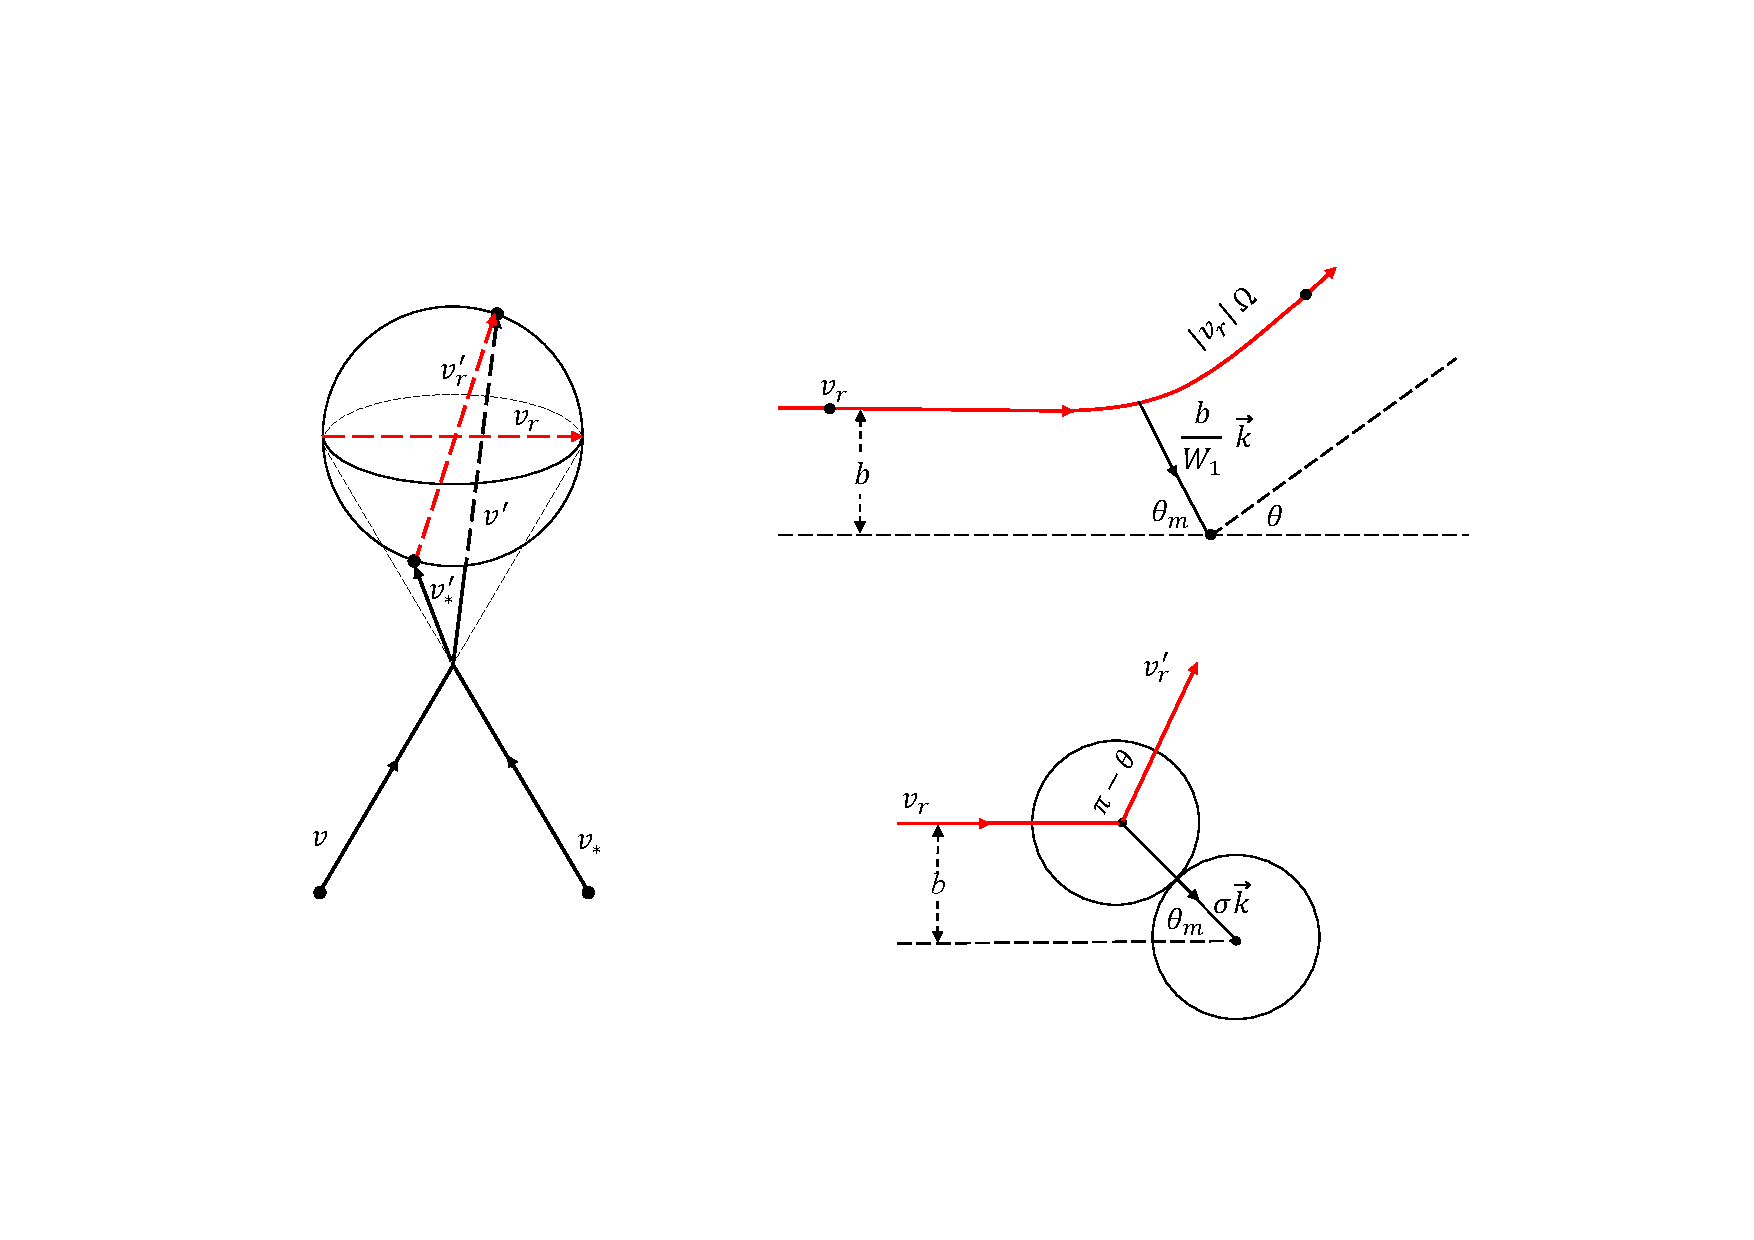
\includegraphics[width=0.9\textwidth]{Fig/Boltzmann_collision_demo.pdf}
	\caption{(左) 二体碰撞前后的速度分布. 由于动量和能量守恒,碰撞前后的相对速度分布在球体上并且通过球心.(右上)中心力场作用下的经典二体碰撞示意图,其中$b$ 为瞄准距离,$\bm{k}$ 为沿两分子间最短距离方向的单位矢量.(右下)直径为$\sigma$ 的硬球分子的两体碰撞.
	}
	\label{Boltzmann_collision_demo}
\end{figure}




\subsection{偏转角和微分散射截面}


假设分子间通过中心力场作用,作用势$\phi(r)$已知, 其中$r$为分子间距,则偏转角可以通过经典力学和量子力学两种方式求解.  若气体温度不低~(如氦气的温度高于100~K),两种方式得到的输运系数(如粘性和热导率)相同\cite{Sharipov2018Vacuum}. 这里仅介绍经典力学的计算结果,如图~\ref{Boltzmann_collision_demo}所示,偏转角可以表示为:
\begin{equation}\label{deflection}
\theta(b,{v}_r)=\pi-2\int_0^{W_1}\left[1-W^2-\frac{4\phi(r)}{m{v}_r^2}\right]^{-1/2}dW,
\end{equation}
其中,$W=b/r$为瞄准距离$b$与分子间距$r$的比值, 积分上限$W_1$对应于最短分子间距,即上式中括号内表达式等于零的方程的正根. 


%碰撞的微分散射截面为
%\begin{equation}\label{DCS_chapter1}
%\sigma_D=\frac{b|db|}{\sin\theta|d\theta|}=\left(\frac{m(\eta-1)}{4K}\right)^{2\eta-2}v^{-\frac{4}{\eta-1}}_r\times\frac{sds}{\sin\Theta{d\Theta}},
%\end{equation}
%碰撞核为
%\begin{equation}
%B(\theta,{v}_r)=v_r\sigma_D.
%\end{equation}


%although the Lennard-Jones potential is widely used (say, in the MD simulation of monatomic gas):
%\begin{equation}\label{Lennard_Jones_chapter}
%\phi(r_{ij})=4\epsilon\left[\left(\frac{d_{LJ}}{r_{ij}}\right)^{12}-\left(\frac{d_{LJ}}{r_{ij}}\right)^6\right],
%\end{equation}

%where $\epsilon$ is the potential depth and $d_{LJ}$ is the distance between two molecules where the potential is zero. 

在气体动理论中,经常考虑如下形式的逆幂律分子作用势:
\begin{equation}\label{power_law_potential}
\phi(r)=\frac{K}{\eta-1}r^{1-\eta},
\end{equation}
其中, $K$表征分子间相互作用的强度.  从公式~\eqref{deflection} 可知,偏转角只与变量$s$有关,即$\theta=\Theta(s)$:
\begin{equation}\label{impact_norm}
s=\left[\frac{m(\eta-1)}{4K}\right]^{\frac{1}{\eta-1}}bv^{\frac{2}{\eta-1}}_r.
\end{equation}

微分散射截面定义为
\begin{equation}\label{DCS_chapter1}
\begin{aligned}[b]
\sigma_D&=\frac{b|db|}{\sin\theta|d\theta|}\\
&=\left(\frac{m(\eta-1)}{4K}\right)^{\frac{2}{1-\eta}}v^{\frac{4}{1-\eta}}_r
\frac{sds}{\sin\Theta{d\Theta}},
\end{aligned}
\end{equation}
而碰撞核为
\begin{equation}
B(\theta,v_r)=v_r \sigma_D.
\end{equation}


当公式\eqref{power_law_potential}中$\eta=5$时,即为麦克斯韦分子,此时碰撞核与相对碰撞速度无关,记为 $B(\theta,v_r)=\sqrt{2K/m}B(\theta)$. 
对于硬球分子模型,可看作式\eqref{power_law_potential}中$\eta=\infty $,从图~\ref{Boltzmann_collision_demo}可以看出,偏转角可通过如下公式确定:
$b=\sigma\cos\left({\theta}/{2}\right)$,其中$\sigma$为硬球直径. 因此微分散射截面为 $\sigma_D={{\sigma}^2}/{4}$,而碰撞核为 $B(\theta,{v}_r)={\sigma}^2v_r/4$.  对于一般的气体,它们的行为介于麦克斯韦分子和硬球分子之间. 




\subsection{熵增原理}


对于任意关于分子速度的函数$\Psi(\bm{v})$,对玻尔兹曼碰撞项~\eqref{chapter1_collision} 在速度空间积分,具有如下对称性:
\begin{equation}\label{symmetry_collision}
\begin{aligned}[b]
\int\Psi(\bm{v})Q(\bm{v})d\bm{v}=&\frac{1}{4}\iiint d\Omega
d\bm{v}_\ast{d\bm{v}}
\Delta[\Psi]
B(\theta,v_r)\\
&\times \left[f(\bm{v}'_{\ast})f(\bm{v}')-f(\bm{v}_{\ast})f(\bm{v})\right],
\end{aligned}
\end{equation}
其中
$\Delta[\Psi]=
\Psi(\bm{v}_{\ast})+\Psi(\bm{v})
-\Psi(\bm{v}'_{\ast})-\Psi(\bm{v}')$. 
若$\Psi$满足 $\int\Psi(\bm{v})Qd\bm{v}=0$,则称其为碰撞不变量. 根据质量、动量和能量守恒,可知 $\Psi=1,\bm{v}, v^2$ 为碰撞不变量,而碰撞不变量的线性组合也是碰撞不变量. 

定义 $H$ 函数为:
\begin{equation}\label{entropy_function}
H=-\iint {f\ln}fd\bm{v}d\bm{x},
\end{equation}
是与气体系统的熵相关的标量.  在无外力的情况下,$H$ 的时间导数可写为:
\begin{equation*}
\begin{aligned}[b]
\frac{\partial H}{\partial t}=&	-\iint(1+{\ln}f)\frac{\partial{f}}{\partial{t}}d\bm{v}d\bm{x}\\
=&\iint{\bm{v}\cdot\frac{\partial{f}\ln{f}}{\partial\bm{x}}}d\bm{v}d\bm{x}-\iint(1+\ln{f}){Q} d\bm{v}d\bm{x}\\
=&\oint \int{\bm{v}\cdot\bm{n} {f}\ln{f}}d\bm{v}dS-\iint(1+\ln{f}){Q} d\bm{v}d\bm{x}.
\end{aligned}
\end{equation*}
式中,$\bm{n}$ 为系统表面微元 $dS$ 的外法线.  对于孤立系统,上式右端第一项为零;利用方程~\eqref{symmetry_collision},右端项第二项可写为:
\begin{equation*}
\begin{aligned}[b]
\frac{1}{4}\iiint{}&d\Omega
d\bm{v}_\ast{d\bm{v}}
B
\left[f(\bm{v}'_{\ast})f(\bm{v}')-f(\bm{v}_{\ast})f(\bm{v})\right]\\
&\times
\left\{
\ln[f(\bm{v}'_{\ast})f(\bm{v}')]
-\ln[f(\bm{v}_{\ast})f(\bm{v})]
\right\}.
\end{aligned}
\end{equation*}
因为碰撞核$B$非负,且对于任意的两个正整数 $a$ 和 $b$,不等式 $(a-b)(\ln{a}-\ln{b})\ge0$ 恒成立, 所以有
\begin{equation}\label{entropy_inequality}
\frac{\partial H}{\partial t}\ge0.
\end{equation}

上式表明孤立系统的$H$函数不会减小,这就是著名的玻尔兹曼的熵增原理. $H$随时间单调增加,但存在有限的上界,上界对应为式~\eqref{entropy_inequality}中等号成立时的平衡态, 即
$\ln{f}(\bm{v}_{\ast})+\ln{f}(\bm{v})
=\ln{f}(\bm{v}'_{\ast})+\ln{f}(\bm{v}')$. 
因此,$\ln{f}$ 也是碰撞不变量,可以表示为五个基本碰撞不变量 的线性组合:
$\ln{f}=\alpha_1+\bm{\alpha}_2\cdot\bm{v}+\alpha_3v^2$;给定系统的密度、速度和温度,
参数$\alpha_1$, $\alpha_3$ 和$\alpha_2$ 可以唯一确定. 此时,麦克斯韦平衡态速度分布函数为
\begin{equation}\label{equilibrium_Maxwellian}
F_{eq}(T)=n\left(\frac{m}{2\pi   k_BT}\right)^{3/2}\exp\left(-\frac{mc^2}{2k_BT}\right).
\end{equation}


\subsection{线性化玻尔兹曼方程}\label{LBE_chapter1}

线性化玻尔兹曼方程在气体动理论中具有重要地位. 第一,线性化玻尔兹曼碰撞项的本征值与本征函数,不仅在渐近展开推导纳维-斯托克斯方程的过程中至关重要,而且是发展简化动理学模型方程的源头理论. 第二,在许多微机电系统中,气体的压力梯度与温度梯度非常小,因此使用线性化方程可以高效准确地模拟微流动. 第三,虽然玻尔兹曼方程是单粒子速度分布函数确定性演化的平均方程,但是在某些问题中(例如:第\ref{RBS_section}节中的瑞利-布里渊散射)可以通过线化玻尔兹曼方程研究粒子涨落带来的影响. 

通常将速度分布函数在全局平衡态
\begin{equation}
f_{eq}=n_0\left(\frac{m}{2\pi   k_BT_0}\right)^{3/2}\exp\left(-\frac{mv^2}{2k_BT_0}\right)
\end{equation}
下展开为
\begin{equation}\label{chapter_vdf_lin_origin}
f(t,\bm{x},\bm{v})=f_{eq}(\bm{v})\left[1+\phi(t,\bm{x},\bm{v})\right],
\end{equation} 
其中扰动量 $\phi$ 满足约束条件 $|\phi|\ll1$. 不考虑外力项,只保留$\phi$的一次项,玻尔兹曼方程~\eqref{Boltzmann}可线性化为如下形式:
%\begin{widetext}
\begin{equation}\label{Chapter1_Boltzmann_lin0}
\begin{aligned}[b]
\frac{\partial\phi}{\partial t}+\bm{\xi}\cdot\frac{\partial\phi}{\partial
	\bm{x}}
&=\frac{\ell}{v_m}{J}(\phi)\\
&\equiv
-\frac{\ell}{v_m}\iint
B
\Delta[\phi]f_{eq}(\bm{v}_{\ast})d\Omega
d\bm{v}_\ast. %-\frac{2}{v_m}\bm{a}\cdot\bm{v}
\end{aligned}
\end{equation}
%\end{widetext}
这里的 速度 和 空间坐标分别通过最概然速率 $v_m$和特征尺寸 $\ell$ 进行无量纲化,时间用$\ell/v_m$归一化;无量纲分子速度为
\begin{equation}
\bm{\xi}=\frac{\bm{c}}{v_m(T_0)},
\end{equation}
其中
\begin{equation}
v_m(T)=\sqrt{\frac{2k_BT}{m}}
\end{equation}
为气体分子的最概然速率,即与麦克斯韦速率分布的极大值对应的速率. 

%\subsubsection{麦克斯韦气体:特征值和特征函数}
%\subsubsection{Maxwellian gas: eigenvalues and eigenfunctions}

对于麦克斯韦分子,线性化玻尔兹曼碰撞项的本征值与本征函数为~\cite{WangCS}:
\begin{equation}\label{Wang_Chang}
\begin{aligned}[b]
{J}(\Phi_{rlm})=&n\lambda_{rl}\Phi_{rlm},\\
\Phi_{rlm}=&g_{rl}(\xi)Y^m_{l}(\hat{\xi})
\\
=&\sqrt{\frac{2\pi^{3/2}r!}{\left(r+l+\frac{1}{2}\right)!}}
S^{(r)}_{l+\frac{1}{2}}(\xi^2)
\xi^l
Y^m_{l}(\hat{\xi}),\\
\lambda_{rl}=&2\pi\sqrt\frac{2K}{m}\int_0^\pi{}d\theta\sin\theta{B(\theta)}\\
&\times\left[-1+\cos^{2r+l}\frac{\theta}{2} 
P_l\left(\cos\frac{\theta}{2}\right) \right.\\
&\left. -\delta_{r0}\delta_{l0}+\sin^{2r+l}\frac{\theta}{2} 
P_l\left(\sin\frac{\theta}{2}\right)
\right].
\end{aligned} 
\end{equation}
式中,$P_l(x)$ 是勒让德多项式,$S^{(r)}_{l+\frac{1}{2}}(\xi)$ 是索南多项式,$Y^m_{l}(\hat{\xi})$ 为 $\bm{\xi}$方向的球谐函数. 


前三项本征值为 $\lambda_{00}=\lambda_{01}=\lambda_{10}=0$,分别代表三大守恒律. 另外两个非常重要的本征值为
\begin{equation}\label{eigenvalues}
\begin{aligned}[b]
\lambda_{02}=\left(-\frac{3}{2}\right)\pi\sqrt\frac{2K}{m}\int_0^\pi{d\theta}\sin^3\theta B(\theta), \\
\lambda_{11}=\frac{2}{3}\lambda_{02}, 
\end{aligned}
\end{equation}
它们决定剪切粘性系数和热导率的大小. 若归一化的速度$\bm{\xi}$在$z$轴的投影为$\xi_z=\xi\cos\theta$, 其中$\theta$为极距角,与上述本征值对应的本征函数为:
\begin{equation*}\label{eigenfunctions}
\begin{aligned}[b]
\Phi_{000}=1, ~
\Phi_{010}=\sqrt{2}\xi_z, ~
\Phi_{100}=\sqrt{\frac{2}{3}}\left(\frac{3}{2}-\xi^2\right), \\
\Phi_{020}=\frac{1}{3\sqrt{3}}\left(\xi^2_z-\frac{\xi^2}{3}\right),\\
\Phi_{110}=\frac{2}{\sqrt{5}}\left(\frac{5}{2}-\xi^2\right)\xi_z.
\end{aligned}
\end{equation*}
它们与气体的分子数密度、速度、温度、压力 和热流的扰动密切相关:
\begin{equation}\label{MP_KineticModel}
\begin{aligned}[b]
&[{n},\bm{u}, T]=\int\left[1,\bm{\xi},\frac{2}{3}\left(\xi^2-\frac{3}{2}\right)\right]
{f_{eq}\phi}d\bm{\xi}, \\
&[\sigma_{ij},\bm{q}]=\int
\left[2\xi_{\langle i}\xi_{j\rangle}, \left(\xi^2 -\frac{5}{2}\right)\bm{\xi}\right]
f_{eq}\phi{}d\bm{\xi}.
\end{aligned}
\end{equation}
其中,下标中出现尖括号表示该张量是无迹张量,即$\xi_{\langle i}\xi_{j\rangle}=\xi_i\xi_j-\xi^2\delta_{ij}/3$. 
为避免使用过多符号,在线性化问题中我们使用与原物理量相同的符号表示归一化的扰动物理量,如这里的扰动数密度$n$应理解为偏离参考数密度$n_0$的那部分,再除以参考数密度; 扰动温度$T$为偏离参考温度$T_0$的部分,再除以参考温度; 在全局平衡态下,参考速度、应力偏量和热流全部为零,因此上式中它们分别以$T_0$下的最概然速率$v_m$、$n_0k_BT_0$和 $n_0k_BT_0v_m$归一化. 

%;另外,我们默认在平衡态上进行扰动,因此参考速度、应力偏量和热流均为零
%\begin{equation}\label{MP_KineticModel}
%\begin{aligned}[b]
%{n}=\int{f_{eq}\phi}d\bm{v}, \\
%\bm{u}=\frac{1}{n_0}\int{\bm{v}f_{eq}\phi}d\bm{v}, \\
%T=\frac{2T_0}{3n_0}\int{\left(\frac{v^2}{v_m^2}-\frac{3}{2}\right)}
%f_{eq}\phi{}d\bm{v},  \\
%\sigma_{ij}=m\int
%v_{\langle i}v_{j\rangle}
%f_{eq}\phi{}d\bm{v}, \\
%\bm{q}=k_BT_0\int\left(\frac{v^2}{v_m^2} -\frac{5}{2}\right)\bm{v} f_{eq}\phi d\bm{v},
%\end{aligned}
%\end{equation}

\subsection{输运系数和弛豫率:表象与本质}

玻尔兹曼方程和纳维-斯托克斯方程分别在介观和宏观尺度上描述气体系统的演化,它们之间的关系一直是数学家和力学家研究的重要课题\cite{Sone2002Book}.  对玻尔兹曼方程求守恒量$m, m\bm{c},mc^2/2$的矩,可以得到如下宏观方程组:
\begin{equation}\label{macro}
\begin{aligned}[b]
\frac{\partial \rho}{\partial t}+\frac{\partial(\rho{}u_j) }{\partial x_j}=0, \\
\frac{\partial (\rho{u_i})}{\partial t}+\frac{\partial (\rho{}u_iu_j+p_{ij})}{\partial x_j}= \rho{}a_i,\\
\frac{\partial \left(\rho{}E\right)}{\partial t}+\frac{\partial \left(\rho{}{E}u_j+u_i{p}_{ij}+q_j\right)}{\partial x_j}=\rho{}a_ju_j,
\end{aligned}
\end{equation} 
其中$E=3k_BT/2m+u^2/{2}$. 但是该方程组并不封闭,因为压力张量和热流的表达式不能用密度、速度和温度表示.  有三种主要方法尝试封闭宏观方程组,它们分别是希尔伯特展开法\cite{Hilbert1912},Chapman-Enskog展开法~\cite{Chapman1916,enskog1917,CE}和矩方法\cite{Grad1949,henning}. 这里我们介绍最常用的第二种方法. 

在Chapman 和 Enskog~\cite{Chapman1916,enskog1917}方法中,首先将玻尔兹曼方程改写为:
\begin{equation}\label{expansion0}
\frac{\partial f}{\partial t}+\bm{v}\cdot\frac{\partial f}{\partial
	\bm{x}}+\bm{a}\cdot\frac{\partial f}{\partial \bm{v}}=\frac{Q(f)}{\epsilon}.
\end{equation} 
然后将分布函数和玻尔兹曼碰撞项展开为$\epsilon$ 的幂级数:
\begin{equation}\label{expansion1}
\begin{aligned}[b]
f=&\sum_{k=0}^\infty {\epsilon^k} f^{(k)},\\
Q=&\sum_{k=0}^\infty {\epsilon^k} Q^{(k)}=Q(f^{(0)})
+\epsilon{}{J}(f^{(1)})+O(\epsilon^2).
\end{aligned}
\end{equation}
值得注意的是,$\epsilon$是一个小的形式参数,主要用于监测展开的阶数. 展开完成后,取$\epsilon=1$. 

同时,压力和热流也相应展开如下:
\begin{equation}\label{shere_hilbert}
\begin{aligned}[b]
p_{ij} =\sum_{k=0}^\infty {\epsilon^k} p_{ij}^{(k)}
\equiv \sum_{k=0}^\infty {\epsilon^k} \times{}m\int{}c_ic_jf^{(k)}d\bm{v},
\\  
\bm{q} =\sum_{k=0}^\infty {\epsilon^k} \bm{q}^{(k)}
\equiv \sum_{k=0}^\infty {\epsilon^k} \times{}\frac{m}{2}\int{}\bm{c}c^2f^{(k)}d\bm{v}. 
\end{aligned}
\end{equation}
但是,碰撞不变量对应的宏观量 $C_M=\{\rho,\bm{u}, T\}$ 仅由分布函数的零阶展开决定,即
\begin{eqnarray}
[\rho,\rho\bm{u}, 3k_B\rho{}T]=m\int{}[1,\bm{v},mc^2]f^{(0)}d\bm{v}, \label{density_hilbert}
\end{eqnarray}
而各个高阶展开对$C_M$的贡献均为零,这称为兼容性条件. 


将公式~\eqref{shere_hilbert}代入公式~\eqref{macro},可知时间导数亦可表示为 $\epsilon$ 级数~\cite{henning}
\begin{equation}\label{fast_slow_time}
\frac{\partial}{\partial{} t}=\sum_{k=0}^\infty \epsilon^k \frac{\partial}{\partial{} t_k},
\end{equation}
且对于零阶近似,可得到
\begin{equation}\label{eq123_zerothOrder}
\begin{aligned}[b]
\frac{\partial \rho}{\partial t_0}+\frac{\partial(\rho{}u_j) }{\partial x_j}=0, \\
\frac{\partial (\rho{u_i})}{\partial t_0}+\frac{\partial (\rho{}u_iu_j+nk_BT\delta_{ij})}{\partial x_j}= \rho{}a_i,\\
\frac{\partial \left(\rho{}E\right)}{\partial t_0}+\frac{\partial \left(\rho{}{E}u_j+u_ink_BT\delta_{ij}\right)}{\partial x_j}=\rho{}a_ju_j.
\end{aligned}
\end{equation} 

从公式~\eqref{expansion0}和~\eqref{expansion1}易知$Q(f^{(0)})=0$. 因此,速度分布函数的零阶展开为
\begin{equation}
f^{(0)}=F_{eq}.
\end{equation} 
而速度分布函数的一阶近似$f^{(1)}=F_{eq}\phi$ 满足以下方程~\cite{henning}
%\begin{widetext}
\begin{equation}\label{integral_solution}
\begin{aligned}[b]
&{J}(\phi)=\frac{1}{F_{eq}}\left[\frac{\partial F_{eq}}{\partial t_0}+\bm{v}\cdot\frac{\partial F_{eq}}{\partial
	\bm{x}}+\bm{a}\cdot\frac{\partial F_{eq}}{\partial \bm{v}} \right]\\
&=
2\xi_{\langle{i}} \xi_{j\rangle}
\frac{\partial u_{\langle i}}{\partial x_{j\rangle}}
+\left(\xi^2-\frac{5}{2}\right)\xi_i\sqrt{\frac{2k_BT}{m}}\frac{\partial \ln{T}}{\partial x_i}.
\end{aligned}
\end{equation}
%\end{widetext}
其中,方程的推导过程中用到
\begin{equation*}
\frac{\partial F_{eq}}{\partial t_0}=
\frac{\partial F_{eq}}{\partial C_M}
\frac{\partial C_M}{\partial t_0}, \quad
\frac{\partial F_{eq}}{\partial \bm{x}}=
\frac{\partial F_{eq}}{\partial C_M}
\frac{\partial C_M}{\partial \bm{x}}, 
\end{equation*} 
以及公式~\eqref{eq123_zerothOrder}. 注意公式\eqref{Chapter1_Boltzmann_lin0}中的$f_{eq}$应改写为$F_{eq}$.


积分方程~\eqref{integral_solution}的解可分为齐次部分与非齐次部分,齐次部分满足 ${J}(\phi)=0$,这说明 $\phi$ 必然是碰撞不变量的线性组合,而兼容性条件要求所有线性组合的系数都为零. 非齐次部分满足如下形式
\begin{equation}
\phi=-A(\xi)\xi_i\sqrt{\frac{2k_BT}{m}}\frac{\partial \ln{T}}{\partial x_i}
-B(\xi)\xi_{\langle{i}} \xi_{j\rangle}\frac{\partial u_{\langle i}}{\partial x_{j\rangle}},
\end{equation}
其中,$A(\xi)$ 和 $B(\xi)$ 的解满足
\begin{equation}\label{transport_coefficient_0}
\begin{aligned}[b]
{J}(A\xi_i)&=-\left(\xi^2-\frac{5}{2}\right)\xi_i,
\\
{J}(B\xi_{\langle{i}} \xi_{j\rangle})&=-2\xi_{\langle{i}} \xi_{j\rangle},
\end{aligned}
\end{equation}
且兼容性条件要求$\int \xi^2A(\xi)F_{eq}d\bm{v}=0$. 


一旦得到$A(\xi)$ 和$B(\xi)$,通过一阶展开就可以恢复牛顿粘性定理与傅里叶热传导定理:
\begin{equation}\label{NS_constitutive}
\begin{aligned}[b]
\sigma^{(1)}_{ij}=-2\mu\frac{\partial u_{\langle i}}{\partial x_{j\rangle}},\quad
q^{(1)}_i=-\kappa \frac{\partial T}{\partial x_i},
\end{aligned}
\end{equation} 
且剪切粘性与热导率分别为
\begin{equation}\label{viscosity_original}
\begin{aligned}[b]
\mu=&\frac{2p}{15\pi^{3/2}}\int\exp(-\xi^2)B(\xi)\xi^4d\bm{\xi},
\\
\kappa=&\frac{2p}{3\pi^{3/2}}
\frac{k_B}{m}
\int\exp(-\xi^2)A(\xi)\xi^4
d\bm{\xi}.
\end{aligned}
\end{equation}


一般将$A(\xi)$ 和$B(\xi)$展开为索南多项式级数
\begin{equation}\label{sonine_expansion}
\begin{aligned}[b]
A(\xi)&=-\sum_{r=1}^{n_a}a_rS^{(r)}_{\frac{3}{2}}(\xi^2), \\
B(\xi)&=\sum_{r=0}^{n_b}b_rS^{(r)}_{\frac{5}{2}}(\xi^2),
\end{aligned}
\end{equation}
然后通过公式~\eqref{transport_coefficient_0}和索南多项式的正交性求解输运系数. 对于麦克斯韦分子,取第一项展开可得到准确的剪切粘性和热导率,即取$A(\xi)=a_1(\xi^2-5/2)$和$B(\xi)=b_0$;而对于其它相互作用势,仅考虑第一项展开得到的输运系数的相对误差也不超过2\%. 定义等效黏度截面为:
\begin{equation}
\sigma_{\mu}=\int \frac{B(\theta,v_r)}{v_r}\sin^2\theta {d\Omega},
%=2\pi\int_0^\pi \frac{B(\theta,v_m\eta)}{v_m\eta}\sin^3\theta {d\theta},
\end{equation}
则剪切粘性为
\begin{equation}\label{shear_CE_viscosity0}
\mu=\frac{5\sqrt{\pi{m}k_BT}}{8\left(\frac{m}{4k_BT}\right)^4\int_0^\infty
	{}v_r^7\sigma_{\mu}\exp\left(-\frac{mv^2_r}{4k_BT}\right)dv_r},
\end{equation}
而热导率为
\begin{equation}\label{shear_CE_thermal0}
{\kappa}=\frac{15}{4}\frac{k_B}{m}\mu,
\end{equation}
从而单原子气体的普朗特数为
\begin{equation}\label{Prandtl_number}
\begin{aligned}[b]
\Pr&={c_p}\frac{\mu}{\kappa}\\
&=\frac{5k_B}{2m}\frac{\mu}{\kappa}=\frac{2}{3}.
\end{aligned}
\end{equation}

对于逆幂律分子间相互作用势\eqref{power_law_potential},可以得出气体粘性和温度的关系
\begin{equation}\label{temperature_dependence}
\mu(T)\propto{T^\omega}, \quad
\omega=\frac{\eta+3}{2(\eta-1)},
\end{equation}
其中 $\omega$ 是粘性温度幂指数. 对于麦克斯韦分子和硬球分子,$\omega$ 分别取1和0.5; 对于其它气体,$\omega$一般介于0.5和1之间. 


%\leir{增大公式~\eqref{sonine_expansion}}中 $n_a$ 和 $n_b$ 的值,对结果的影响不大.例如,对于麦克斯韦分子,方程~\eqref{shear_CE_viscosity} 和方程~\eqref{shear_CE_thermal0} 是精确的,而对于硬球分子,当 $n_a=n_b=4$ 时,有
%%The results do not change much if we consider larger values of $n_a$ and $n_b$ in Eq.~\eqref{sonine_expansion}. For examples, for Maxwell molecules, Eqs.~\eqref{shear_CE_viscosity} and~\eqref{shear_CE_thermal0} are exact, while for HS molecules, if we consider $n_a=n_b=4$, we have
%\begin{equation}\label{transport_high_oder}
%\mu^{[4]}=1.016\mu^{[1]}, \\
%\kappa^{[4]}=1.025\kappa^{[1]}.
%\end{equation}
%对于幂指数在 $5\le\eta<\infty$ 范围内的逆幂律分子~\eqref{power_law_potential},修正因子介于麦克斯韦分子和硬球分子之间.

将公式~\eqref{NS_constitutive}代回公式~\eqref{macro}, 即可获得纳维-斯托克斯方程. 若继续计算Chapman-Enskog展开的高阶近似,可以得到Burnett、super-Burnett等宏观方程组\cite{CE}. 但是可能由于应力和热流与宏观量$C_M$展开的不匹配,导致高阶方程组的线性不稳定性. 同时,由于边界条件数量随着方程组阶数升高而增加,但对附加的边界条件提法缺少充分的研究,因此高阶方程组很少被实际应用. 另一方面,即使这些高阶方程组在某些情况下能得到精确解,解的精度也不一定随着展开阶数的增加而增加\cite{Gu2020AIA}. 

值得一提的是,对于麦克斯韦分子,在空间均匀系统中,本征值 $\lambda_{02}$ 和 $\lambda_{11}$ 与应力偏量和热流的弛豫速率相关,而这些弛豫速率决定着剪切粘性系数和热传导的大小:
\begin{equation}\label{universal_relation}
\begin{aligned}[b]
\frac{\partial \sigma_{ij}}{\partial t}
=&-n\lambda_{02} \sigma_{ij}=-\frac{p}{\mu}\sigma_{ij},\\
\frac{\partial q_{i}}{\partial t}=&-n\lambda_{11} q_{i}=-\frac{2}{3}\frac{p}{\mu}q_{i}.
\end{aligned}
\end{equation}
可以认为这些弛豫过程是本质,而粘性系数和热导率则为表象:在稀薄气体流动中,本构关系\eqref{NS_constitutive}和等效输运系数会随着克努森数的改变而改变,但一旦分子作用势确定,弛豫系数就会确定不变. 

利用弛豫时间和输运系数的关系,可以大大简化模型方程中输运系数的推导过程.  即,如果应力偏量的弛豫时间为$\tau$, 则剪切粘性为$p\tau$. 如果热流的弛豫时间为$\tau/A$,则普朗特数为$A$. 



% !TeX encoding = UTF-8
% !TeX spellcheck = en_US

\chapter{Fluid-dynamic Equations}
\label{chap:macroscopic}


The derivation of macroscopic equations in closed forms from the Boltzmann equation is of both fundamental and practical importance, since the structure of Boltzmann collision operator is complicated and difficult to handle both theoretically and numerically. And there are huge demanding of macroscopic equations that allow efficient and accurate calculation of rarefied gas dynamics with applications from aerodynamics to microfludics. It has also been considered as an important part in the sixth Hilbert problem: ``Thus Boltzmann's work on the principles of mechanics suggests the problem of developing mathematically the limiting processes, which lead from the atomistic view to the laws of motion of continua''~\cite{Hilbert1902}. In this Chapter we first introduce how macroscopic equations are derived, and then assess the their accuracy. % in the problems of Rayleigh-Brillouin scattering and sound wave damping. 


\section{Hilbert expansion}

Macroscopic equations like Eq.~\eqref{macro} can be obtained by multiplying the Boltzmann equation~\eqref{Boltzmann} with the collision invariants and integrating with respect to the molecular velocity $\bm{v}$. However, the obtained moment system is not closed because expressions for the stress and heat flux are not known. Hilbert proposed to solve the Boltzmann equation via a formal asymptotic expansion of the VDF as~\cite{Hilbert1912}:
\begin{equation}\label{asymptotic}
f(t,\bm{x},\bm{v})=\sum_{n=0}^\infty {\epsilon^n} f^{(n)}(t,\bm{x},\bm{v}),
\end{equation}
where $\epsilon$ is a formal small parameter which plays the role of spatial Knudsen number for monitoring the order of terms and quantities appearing in the equations, which will be replaced by one when the solutions are obtained. Meanwhile, the Boltzmann collision operator is written as
\begin{equation}
\frac{Q}{\epsilon}=\sum_{n=0}^\infty {\epsilon^{n-1}} Q^{(n)}, 
\end{equation} 
where $Q^{(0)}=Q(f^{(0)},f^{(0)})$ and $Q^{(1)}=f^{(0)}\mathcal{J}(\phi)$ if we write $f^{(1)}=f^{(0)}\phi$.

The macroscopic variables are also expressed into the power series of $\epsilon$ according to Eq.~\eqref{macroscopic_origin}:
\begin{equation}\label{conservative_hilbert}
\begin{aligned}[b]
\left[\rho,\rho\bm{u},\frac{3}{2}k_B\rho{}T\right]=\sum_{n=0}^\infty \epsilon^n \int \left[1,\bm{v}, \frac{1}{2}mc^2\right]mf^{(n)}d\bm{v},
\end{aligned}
\end{equation} 
and
\begin{equation}\label{shere_hilbert}
\begin{aligned}[b]
p_{ij} &=\sum_{n=0}^\infty \epsilon^n p_{ij}^{(n)},
\quad
p^{(n)}_{ij}=\int{}mc_ic_jf^{(n)}d\bm{v}
 \\  
 \bm{q} &=\sum_{n=0}^\infty \epsilon^n \bm{q}^{(n)}, 
 \quad
 \bm{q}^{(n)}=\int{}\frac{1}{2}mc^2\bm{c}f^{(n)}d\bm{v}.
 \end{aligned}
\end{equation}

Substituting Eq.~\eqref{asymptotic} into the Boltzmann equation and collecting powers of $\epsilon$ yields an infinite system of integro-differential equations for $f^{(n)}$. At the order $O(\epsilon^{-1})$ we have $Q^{(0)}=0$.
Therefore, $f^{(0)}$ is the equilibrium distribution function~\eqref{equilibrium_Maxwellian}:
\begin{equation}
f^{(0)}
=\frac{\rho^{(0)}}{m}\left(\frac{m}{2\pi   k_BT^{(0)}}\right)^{3/2}\exp\left(-\frac{m(\bm{v}-\bm{u}^{(0)})^2}{2k_BT^{(0)}}\right),
\end{equation}
but the density, velocity and temperature are evaluated at the zeroth-order expansion, e.g., $\rho^{(0)}=\int {mf^{(0)}d\bm{v}}$. 
If only this zeroth-order expansion is adopted, we have  $\rho^{(0)}=\rho$, $\bm{u}^{(0)}=\bm{u}$, and $T^{(0)}=T$. Therefore, the corresponding set of macroscopic equations are the Euler equations, i.e., Eq.~\eqref{macro} with
$p_{ij}=nk_BT\delta_{ij}$ and $\bm{q}=0$. When the first-order expansion in VDF is considered: $f=f^{(0)}+f^{(0)}\phi$, we have 
\begin{equation}\label{Q1_Hilbert}
f^{(0)}\mathcal{J}(\phi)= 
\frac{\partial f^{(0)}}{\partial t}+\bm{v}\cdot\frac{\partial f^{(0)}}{\partial
	\bm{x}}+\bm{a}\cdot\frac{\partial f^{(0)}}{\partial \bm{v}}.
\end{equation}
%In this case, $f^{(0)}$ is still given by the equilibrium VDF $F_{eq}$,
By solving Eq.~\eqref{Q1_Hilbert}, one can obtain $\phi$ and hence $f^{(1)}$; and the process can be carried on to obtain high-order approximations. We refer to the monograph of Sone~\cite{Sone2002Book} for more details. However, it should be noted that the NSF equations never emerge according to the Hilbert expansion.



\section{Chapman-Enskog expansion}\label{Champan_Enskog_expansion}
\index{Chapman-Enskog expansion}
\index{Chapman-Enskog expansion!Navier-Stokes-Fourier equations}

Chapman and Enskog independently proposed a new technique~\cite{Chapman1916,Enskog1917}, which has become the standard procedure to derive macroscopic equations from the kinetic equation. The most successful part is that the transport coefficients in NSF equations can be derived as long as the intermolecular potential is known. In the Chapman-Enskog expansion, the VDF, stress and heat flux remain the same as the Hilbert expansion. However, the five conservative variables $C_M=\{\rho,\bm{u}, T\}$  are calculated only according to the zeroth-order expansion. That is, 
\begin{eqnarray}\label{density_hilbert}
\left[\rho,\rho\bm{u},\frac{3}{2}k_B\rho{}T\right]=
m\int{}\left[1,\bm{v},\frac{1}{2}mc^2\right]f^{(0)}d\bm{v},  
\end{eqnarray}
with the compatibility condition
\begin{eqnarray} \label{compatibility}
\int{}f^{(n)}d\bm{v}=\int{}\bm{v}f^{(n)}d\bm{v}=\int{}c^2f^{(n)}d\bm{v}=0, \quad \text{for} \quad n\ge1.
\end{eqnarray}


On substituting the above equations to Eq.~\eqref{macro}, one finds that the time derivatives is formally written as a series in $\epsilon$~\cite{henning}:
\begin{equation}\label{fast_slow_time}
\frac{\partial}{\partial{} t}=\sum_{n=0}^\infty \epsilon^n \frac{\partial}{\partial{} t_n}.
\end{equation}
Therefore, at the zeroth-order approximation, we have
\begin{equation}\label{eq123_zerothOrder}
\begin{aligned}[b]
\frac{\partial \rho}{\partial t_0}+\frac{\partial(\rho{}u_j) }{\partial x_j}=0, \\
\frac{\partial (\rho{u_i})}{\partial t_0}+\frac{\partial (\rho{}u_iu_j+nk_BT\delta_{ij})}{\partial x_j}= \rho{}a_i,\\
\frac{\partial \left(\rho{}E\right)}{\partial t_0}+\frac{\partial \left(\rho{}{E}u_j+u_ink_BT\delta_{ij}\right)}{\partial x_j}=\rho{}a_ju_j,
\end{aligned}
\end{equation} 
while at other orders $(n>0)$ we have
\begin{equation}\label{eq123_HighOrder}
\begin{aligned}[b]
\frac{\partial \rho}{\partial t_n}=0, \quad
\frac{\partial (\rho{u_i})}{\partial t_n}+\frac{\partial p^{(n)}_{ij}}{\partial x_j}= 0,\quad
\frac{\partial \left(\rho{}E\right)}{\partial t_n}+\frac{\partial \left(u_ip^{(n)}_{ij}+q^{(n)}_j\right)}{\partial x_j}=0.
\end{aligned}
\end{equation} 

%The Maxwellian $F_{eq}$ depends on the conservative variables and the above expansion can be used to expand its time derivative according to 
%\begin{equation}
%\frac{DF_{eq}}{Dt}=\frac{DF_{eq}}{Dt_0}+\epsilon\frac{DF_{eq}}{Dt_1}+\cdots,
%\end{equation}
%where 
%\begin{equation}
%\frac{DF_{eq}}{Dt_\epsilon}=
%\frac{\partial F_{eq}}{\partial C_M}
%\frac{\partial C_M}{\partial t_\epsilon}.
%\end{equation}


%\subsection{Transport coefficients}
\index{transport coefficient}
\index{shear viscosity}
\index{thermal conductivity}


At the order $O(\epsilon^{-1})$, like the Hilbert expansion, we have $Q(f^{(0)},f^{(0)})=0$. Hence $f^{(0)}$ is just the equilibrium distribution function~\eqref{equilibrium_Maxwellian}, because the conservative variables $C_M$ are determined only according to the zeroth-order expansion. 

At the order $O(1)$, the VDF $f^{(1)}=F_{eq}\phi$ satisfies the following equation:
\begin{equation}\label{integral_solution}
\begin{aligned}[b]
F_{eq}\mathcal{J}(\phi)=&\frac{\partial F_{eq}}{\partial t_0}+\bm{v}\cdot\frac{\partial F_{eq}}{\partial
	\bm{x}}+\bm{a}\cdot\frac{\partial F_{eq}}{\partial \bm{v}}\\
=&\left[
2\xi_{\langle{i}} \xi_{j\rangle}
\frac{\partial u_{\langle{i}}}{\partial x_{j\rangle}}
+\left(\xi^2-\frac{5}{2}\right)\xi_i\sqrt{\frac{2k_BT}{m}}\frac{\partial \ln{T}}{\partial x_i}
\right]F_{eq}.
\end{aligned}
\end{equation}
Note that the final equation is obtained with the help of $\frac{\partial F_{eq}}{\partial t_0}=
\frac{\partial F_{eq}}{\partial C_M}
\frac{\partial C_M}{\partial t_0}$,  $\frac{\partial F_{eq}}{\partial \bm{x}}=
\frac{\partial F_{eq}}{\partial C_M}
\frac{\partial C_M}{\partial \bm{x}}$, and Eq.~\eqref{eq123_zerothOrder}. Details can be found in Struchtrup's book~\cite{henning}.

The solution of the integral equation~\eqref{integral_solution} can be decomposed into a homogeneous part and inhomogeneous part. The homogeneous part of solution satisfied $\mathcal{J}(\phi)=0$, thus $\phi$ must be linear combinations of collisional invariants. However, the compatibility condition~\eqref{compatibility} requires that all the combination coefficients are zero. The inhomogeneous solution must be read
\begin{equation}
\phi=
-A_\mu(\xi)\xi_{\langle{i}} \xi_{j\rangle}\frac{\partial u_{\langle{i}}}{\partial x_{j\rangle}}
-A_\kappa(\xi)\xi_i\sqrt{\frac{2k_BT}{m}}\frac{\partial \ln{T}}{\partial x_i},
\end{equation}
where $\int \xi^2A_\kappa(\xi)F_{eq}d\bm{v}=0$ for the compatibility condition~\eqref{compatibility}, and the solutions of $A_\kappa(\xi)$ and $A_\mu(\xi)$ satisfy
\begin{equation}\label{transport_coefficient_0}
\begin{aligned}[b]
\mathcal{J}(A_\mu\xi_{\langle{i}} \xi_{j\rangle})&=-2\xi_{\langle{i}} \xi_{j\rangle},
\text{~and~}
\mathcal{J}(A_\kappa\xi_i)&=-\left(\xi^2-\frac{5}{2}\right)\xi_i.
\end{aligned}
\end{equation}


Once $A_\kappa(\xi)$ and $A_\mu(\xi)$ are known, Newton's law for stress and Fourier's law for heat conduction can be obtained:
\begin{equation}
\begin{aligned}[b]
\sigma^{(1)}_{ij}=-2\mu\frac{\partial u_{\langle i}}{\partial x_{j\rangle}},
\text{~and~}
q^{(1)}_i=-\kappa \frac{\partial T}{\partial x_i},
\end{aligned}
\end{equation} where the shear viscosity and heat conductivity are
\begin{equation}\label{viscosity_original}
\begin{aligned}[b]
\mu=&\frac{2p}{15\pi^{3/2}}\int\exp(-\xi^2)A_\mu(\xi)\xi^4d\bm{\xi},
\\
\kappa=&\frac{2p}{3\pi^{3/2}}
\frac{k_B}{m}
\int\exp(-\xi^2)A_\kappa(\xi)\xi^4
d\bm{\xi}.
\end{aligned}
\end{equation}

The NSF equations are obtained by combining Eqs.~\eqref{fast_slow_time}, \eqref{eq123_zerothOrder} and \eqref{eq123_HighOrder} with $n=1$, which is accurate to $O(\text{Kn})$. 


%\subsubsection{Variational solution}

\subsubsection{Expansion in Sonine polynomials}

Although Eq.~\eqref{transport_coefficient_0} can be solved exactly by the fast spectral method so that the transport coefficients in Eq.~\eqref{viscosity_original} can be calculated exactly (see Section~\ref{accurate_transport}), an analytical derivation will be beneficial. 

With the Sonine polynomials in Appendix~\ref{appendix_special_functions}, the integral equation~\eqref{transport_coefficient_0} can be written as $\mathcal{J}(A_\kappa\xi_i)=S^{(1)}_{\frac{3}{2}}(\xi^2)\xi_i$ and $\mathcal{J}(A_\mu\xi_{\langle{i}}\xi_{j\rangle})=-2S^{(0)}_{\frac{5}{2}}(\xi^2) \xi_{\langle{i}}\xi_{j\rangle}$. For their solution, $A_\kappa(\xi)$ and $A_\mu(\xi)$ are expanded as
\begin{equation}\label{sonine_expansion}
\begin{aligned}[b]
A_\kappa(\xi)=-\sum_{r=1}^{n_a}a_rS^{(r)}_{\frac{3}{2}}(\xi^2), 
\text{~and~}
A_\mu(\xi)=\sum_{r=0}^{n_b}b_rS^{(r)}_{\frac{5}{2}}(\xi^2).
\end{aligned}
\end{equation}





Multiplying Eq.~\eqref{transport_coefficient_0} with $\exp(-\xi^2)S^{(s)}_{\frac{3}{2}}(\xi^2)\xi_i$ and $\exp(-\xi^2)S^{(s)}_{\frac{5}{2}}(\xi^2)\xi_{\langle{i}}\xi_{j\rangle}$, respectively, and  taking advantage of the orthogonality of Sonine's polynomials, we have
\begin{equation}
\begin{aligned}[b]
&\sum_{r=1}^{n_a}\alpha_{sr}a_r=\frac{15}{4}\pi^3\frac{m}{\rho}\delta_{s1}, \quad
&\sum_{r=1}^{n_a}\beta_{sr}b_r=5\pi^3\frac{m}{\rho}\delta_{s0},
\end{aligned}
\end{equation} 
%\begin{equation}
%\begin{aligned}[b]
%&\sum_{r=1}^{n_a}\alpha_{sr}a_r=\frac{15}{4}\pi^3\frac{m}{\rho}\delta_{s1} \Longrightarrow
%a_r=\frac{15}{4}\pi^3\frac{m}{\rho}\alpha^{-1}_{r1},\\
%&\sum_{r=1}^{n_a}\beta_{sr}b_r=5\pi^3\frac{m}{\rho}\delta_{s0} \Longrightarrow
%b_r=5\pi^3\frac{m}{\rho}\beta^{-1}_{r0},
%\end{aligned}
%\end{equation} 
where the matrices $\alpha_{sr}$ and $\beta_{sr}$ are
\begin{equation}
\begin{aligned}[b]
\alpha_{sr}=\left[S^{(s)}_{\frac{3}{2}}(\xi^2)\xi_i,S^{(r)}_{\frac{3}{2}}(\xi^2)\xi_i\right],\quad
\beta_{sr}=\left[S^{(s)}_{\frac{5}{2}}(\xi^2)\xi_{\langle{i}}\xi_{j\rangle},S^{(r)}_{\frac{5}{2}}(\xi^2)\xi_{\langle{i}}\xi_{j\rangle}\right],
\end{aligned}
\end{equation}
with the bracket operator defined in Eq.~\eqref{integral_equation}.

Note that with the compatibility equation the last equation in Eq.~\eqref{viscosity_original} can be rewritten as
	$
	\kappa=\frac{2p}{3\pi^{3/2}}
	\frac{k_B}{m}
	\int\exp(-\xi^2)A_\kappa(\xi)\xi_i
	\left(\xi^2-\frac{5}{2}\right)
	\xi_i
	d\bm{\xi}$.
Therefore, together with Eq.~\eqref{sonine_expansion}, we have
\begin{equation}\label{viscosity_general_fundamental}
\mu=\frac{p}{2}b_0, 
\quad
\kappa=\frac{p}{2}a_1.
\end{equation}
In order to obtain the analytical expressions for shear viscosity and thermal conductivity, we need to compute $\alpha_{sr}$ and $\beta_{sr}$, and their inverses. %from which we only require the elements $\alpha^{-1}_{11}$ and $\beta^{-1}_{00}$
Their values depend on the numbers of $n_a$ and $n_b$ in Eq.~\eqref{sonine_expansion}. However, for Maxwell molecules, according to Eq.~\eqref{Wang_Chang}, $\alpha_{sr}$ and $\beta_{sr}$ are diagonal, so 
%$\alpha^{-1}_{11}=1/\alpha_{11}$ and $\beta^{-1}_{00}=1/\beta_{00}$.
\begin{equation}\label{viscosity_general}
\mu=\frac{p}{2}b_0=\frac{5\pi^3}{2}k_BT\beta^{-1}_{00}, 
\quad
\kappa=\frac{p}{2}a_1=\frac{75\pi^3}{8}\frac{k_B}{m}k_BT\alpha^{-1}_{11}.
\end{equation}
For other intermolecular potentials, this approximation already give a very accurate estimation of the transport coefficients, as we will see immediately below.





\subsubsection{Expansion to the first-order}


If only one element in each expansion in Eq.~\eqref{sonine_expansion} is used, we get 
\begin{equation}\label{alpha_beta}
\begin{aligned}[b]
\alpha_{11}
=&\frac{1}{4}\int \exp(-\xi^2-\xi^2_\ast)
\mathcal{D}^2(\xi^2\xi_i)B(\cos\theta,v_r)d\Omega{d\bm{\xi}_\ast}d\bm{\xi},\\
\beta_{00}=&\frac{1}{4}\int \exp(-\xi^2-\xi^2_\ast)
\mathcal{D}^2(\xi_{\langle{i}}\xi_{j\rangle})
B(\cos\theta,v_r)
d\Omega{d\bm{\xi}_\ast}d\bm{\xi},
\end{aligned}
\end{equation}
where $\mathcal{D}(\psi)=\psi+\psi_\ast-\psi'-\psi'_\ast$. 

If we define $\eta_i=\xi_i-\xi_{\ast {i}}$, 
$\zeta_i=\frac{1}{2}(\xi_i+\xi_{\ast {i}})=\frac{1}{2}(\xi'_i+\xi'_{\ast {i}})$,  $\eta'_i=\xi'_i-\xi'_{\ast {i}}$, 
 and $v_r=v_m\eta$, we have $\xi^2+\xi^2_{\ast}=2\zeta^2+\frac{1}{2}\eta^2$, ${d\bm{\xi}_\ast}d\bm{\xi}=d\bm{\eta}d\bm{\zeta}$,
${D}(\xi^2\xi_i)=\zeta_i(\eta_i\eta_j-\eta'_i\eta'_j)$, 
$\mathcal{D}(\xi_{\langle{i}}\xi_{j\rangle})=\frac{1}{2}(\eta_i\eta_j-\eta'_i\eta'_j)$. Thus,
\begin{equation*}
\begin{aligned}[b]
\mathcal{D}^2(\xi_{\langle{i}}\xi_{j\rangle})=&\frac{1}{4}(\eta_i\eta_j-\eta'_i\eta'_j)(\eta_i\eta_j-\eta'_i\eta'_j)\\
=&\frac{1}{2}(\eta^4-\eta_i\eta'_i\eta_j\eta'_j)=\frac{1}{2}\eta^4\sin^2\theta,
\end{aligned}
\end{equation*} 
where the last equation is obtained by the fact that the relative velocity is deflected by an angle of $\theta$ after the binary collision, while its magnitude remains unchanged, see Fig.~\ref{Boltzmann_collision_demo}. 


In the calculation of ${D}^2(\xi^2\xi_i)$, if we ignore the terms which have zero contribution to the integral in Eq.~\eqref{alpha_beta}, we have
\begin{equation*}
\begin{aligned}[b]
{D}^2(\zeta^2\zeta_i)=&\zeta^2_1(\eta_1\eta_j-\eta'_1\eta'_j)(\eta_1\eta_j-\eta'_1\eta'_j)+\zeta^2_2(\eta_2\eta_j-\eta'_2\eta'_j)(\eta_2\eta_j-\eta'_2\eta'_j)\\
&+\zeta^2_3(\eta_3\eta_j-\eta'_3\eta'_j)(\eta_3\eta_j-\eta'_3\eta'_j)\\
=&\frac{\zeta^2}{3}(\eta_1\eta_j-\eta'_1\eta'_j)(\eta_1\eta_j-\eta'_1\eta'_j)
+\frac{\zeta^2}{3}(\eta_2\eta_j-\eta'_2\eta'_j)(\eta_2\eta_j-\eta'_2\eta'_j)\\
&+\frac{\zeta^2}{3}(\eta_3\eta_j-\eta'_3\eta'_j)(\eta_3\eta_j-\eta'_3\eta'_j)\\
=&\frac{2}{3}\zeta^2(\eta^4-\eta_i\eta'_i\eta_j\eta'_j)
=\frac{2}{3}\zeta^2\eta^4\sin^2\theta.
\end{aligned}
\end{equation*} 

After integration with respect to $\zeta$ it can be shown that, 
\begin{equation}
\alpha_{11}=\beta_{00}
=\frac{1}{8}\sqrt{\frac{\pi}{2}}^3{4\pi{v_m}}\int_0^\infty\exp\left(-\frac{\eta^2}{2}\right)\eta^7\sigma_{\mu}d\eta,
\end{equation}
where 
\begin{equation}
\sigma_{\mu}=\int \frac{B(\cos\theta,v_r)}{v_r}\sin^2\theta {d\Omega}=2\pi\int_0^\pi \frac{B(\cos\theta,v_m\eta)}{v_m\eta}\sin^3\theta {d\theta},
\end{equation}
is the viscosity cross-section. Therefore, the shear viscosity, which is obtained from Eq.~\eqref{viscosity_general} for the first approximation, is given by
\begin{equation}\label{shear_CE_viscosity0}
\mu^{[1]}=\frac{5\sqrt{\pi{m}k_BT}}{8D},
\end{equation}
where
\begin{equation}\label{shear_CE_viscosity} 
D=\left(\frac{m}{4k_BT}\right)^4\int_0^\infty
v_r^7\sigma_{\mu}\exp\left(-\frac{mv^2_r}{4k_BT}\right)dv_r.
\end{equation}
The corresponding thermal conductivity is given by
\begin{equation}\label{shear_CE_thermal0}
{\kappa}^{[1]}=\frac{15}{4}\frac{k_B}{m}\mu^{[1]},
\end{equation}
which results in a Prandtl number
\begin{equation}\label{Prandtl_number}
\Pr=\frac{\mu{c_p}}{\kappa}=\frac{5k_B}{2m}\frac{\mu}{\kappa}=\frac{2}{3},
\end{equation}
where $c_p$ is the specific heat at constant pressure.

Finally, it is noted that the VDF from the first-order Chapman-Enskog expansion is
\begin{equation*}
\begin{aligned}[b]
f=F_{eq}\left[1-\frac{2m{\kappa}}{5nk_B^2T}\left(\frac{mc^2}{2k_BT} -\frac{5}{2}\right)c_i\frac{\partial \ln{T}}{\partial x_i}
-\frac{m\mu{}}{n{k_B^2}T^2}\frac{\partial u_i}{\partial x_j}c_{\langle i}c_{j\rangle} \right].
\end{aligned}
\end{equation*}



\subsubsection{Expansion to higher-orders}
It turns out that the expansion to first-order is accurate enough for the shear viscosity and thermal conductivity: the results do not change much if we consider larger values of $n_a$ and $n_b$ in Eq.~\eqref{sonine_expansion}.  For example, for inverse power-law potentials~\eqref{power_law_potential}, expansion to the second-order leads to 
\begin{equation*}
\begin{aligned}[b]
\mu^{[2]}&=\left[1+\frac{3(\eta-5)^2}{2(\eta-1)(101\eta-113)}\right]\mu^{[1]}, \\
\kappa^{[2]}&=\left[1+\frac{(\eta-5)^2}{4(\eta-1)(11\eta-13)}\right]\kappa^{[1]}.
\end{aligned}
\end{equation*}

For Maxwell molecules, Eqs.~\eqref{shear_CE_viscosity} and~\eqref{shear_CE_thermal0} are exact, while for HS molecules, if we consider $n_a=n_b=4$, we have
\begin{equation}\label{transport_high_oder}
\mu^{[4]}=1.016\mu^{[1]}, 
\text{~and~}
\kappa^{[4]}=1.025\kappa^{[1]}.
\end{equation}
For inverse power-law potentials~\eqref{power_law_potential} with exponents $5\le\eta<\infty$, the correction factors fall between these for Maxwell and HS molecules.




\subsubsection{Problems of Chapman-Enskog expansion}

The Chapman-Enskog expansion~\cite{CE} leads to respectively the Euler, NS, Burnett, and super-Burnett equations at the zeroth-, first-, second-, and third-order approximations. 
However, it received criticisms because
\begin{itemize}
	\item the Burnett and super-Burnett equations are unstable to perturbation with small wavelength~\cite{Bobylev2006,Colin2008};
	
	% what is the status of the series of the macroscopic variables obtained from the successively derived set of equations nor 
	\item one does not know what step of the approximation is required or sufficient to obtain a solution that is correct up to  $\text{Kn}^n$~\cite{Cercignanibook1988,Sone2002Book}, e.g., the super-Burnett equations are not necessary more accurate than the Burnett equations.
	
\end{itemize} 

Although the augmented Burnett equations~\cite{Zhong1993} solves the instability problem, the second criticism remains. %Later in this chapter we will show that the super-Burnett equations are not necessary more accurate than the Burnett equations, which confirms the unfavorable behavior of successive Chapman-Enskog expansions.


%The second and third expansions lead to the Burnett and super-Burnett equations~\cite{CE,henning}, respectively. In the slip flow regime, the Burnett equations are more accurate than the NSF equations~\cite{Xu2004,Zheng2002}. However, due to its intrinsic instability at large Knudsen numbers~\cite{Colin2008}, it seems that the Burnett and super-Burnett equations are not widely used nowadays. 


\section{Moment methods}
\index{moment equations}
\index{moment equations!Grad 13}
\index{moment equations!Regularized 13}
\index{moment equations!Regularized 26}
% !  ! Regularized 26}


% In his method, the state of a gas is described by a set of moments (e.g., $\rho$, $\bm{u}$, $T$, $\bm{p}$, and $\bm{q}$ are used in Grad 13 method) and the corresponding moment equations are closed by expanding the VDF in Hermite polynomials and assuming this VDF only depends on these moments. 


Another way to obtain the closed macroscopic equations is proposed by Grad~\cite{Grad1949}. In his method, the state of a gas is described by a set of moments (e.g., $\rho$, $\bm{u}$, $T$, $p_{ij}$, and $\bm{q}$ are used in Grad 13 method). In addition to Eq.~\eqref{macro}, he obtained macroscopic equations for the evolution of shear stress and heat flux by respectively multiplying Eq.~\eqref{Boltzmann_dimensionless} with $c_ic_j$ and $c_ic^2$ and integrating over molecular velocity space:
\begin{equation}
\begin{aligned}[b]
\frac{D\sigma_{ij}}{Dt}+ \frac{\partial u^0_{ijk}}{\partial x_k} +\frac{4}{5}\frac{\partial q_{\langle i}}{\partial x_{j\rangle}}
+2\sigma_{k\langle i}\frac{\partial u_{j\rangle}}{\partial x_k} +\sigma_{ij}\frac{\partial u_k}{\partial x_k}+2p\frac{\partial u_{\langle i}}{\partial x_{j\rangle}}=-\frac{p}{\mu}\sigma_{ij}, \\
\frac{Dq_{i}}{Dt}+\frac{5}{2}p\frac{\partial \theta}{\partial x_i} -\sigma_{ik}\frac{\partial\theta}{\partial x_k} -\sigma_{ik}\theta\frac{\partial\ln\rho}{\partial x_k}
-\frac{\sigma_{ik}}{\rho}\frac{\partial\sigma_{kl}}{\partial x_l}
-\frac{5}{2}\theta\frac{\partial\sigma_{ik}}{\partial x_k}
+\frac{1}{2}\frac{\partial u^{1}_{ik}}{\partial x_k}\\
+\frac{1}{6}\frac{\partial w}{\partial x_i}
+u^0_{ijk}\frac{\partial u_k}{\partial x_l}
+\frac{7}{5}q_i\frac{\partial u_k}{\partial x_k}
+\frac{7}{5}q_k\frac{\partial u_i}{\partial x_k}
+\frac{2}{5}q_k\frac{\partial u_k}{\partial x_i}
=-\frac{p}{\mu}q_i,
\end{aligned}
\end{equation}
where $\theta=k_BT/m$, the indices in angular brackets denote the symmetric and trace-free part of a tensor, the terms in the right-hand-side of equation are obtained from the Boltzmann equation for Maxwell molecules, and
\begin{equation}
\frac{D}{Dt}=\frac{\partial}{\partial t}+u_k\frac{\partial }{\partial x_k}
\end{equation}
is the material derivative.


The system is not closed because of the following unknown quantities:
\begin{equation}
\begin{aligned}[b]
[u^0_{ijk},u^1_{ij}]=m\int [c_{\langle i}c_jc_{k\rangle},c^2c_{\langle i}c_{j\rangle}] fd\bm{v}, \quad
w=m\int c^4  (f-F_{eq}) d\bm{v}.
\end{aligned}
\end{equation} 
Grad closed the moment equations by expanding the VDF into the Hermite polynomials of the peculiar velocity, with the coefficients related to the considered low-order moments:
\begin{equation}\label{Grad13VDF}
f=F_{eq}\left[1+\frac{\sigma_{ij}  }{2\rho(k_BT/m)^2}c_{\langle i}c_{j\rangle}
+\frac{2}{5}\frac{q_i}{\rho(k_BT/m)^2}c_i\left(\frac{c^2}{2RT}-\frac{5}{2}\right)\right].
\end{equation}
As a result, $u^0_{ijk}=w=0$ and $u^1_{ij}=7\theta\sigma_{ij}$.




%Grad 13 (G13) equations are accurate to $\text{Kn}^2$~\cite{henning}.  


Similarly, higher-order equations such as the Grad 26 moments equations are constructed by adding more moments to the VDF. Generally speaking, when the rarefaction effects become significant, the number of moments should be increased. For example, for normal shock waves with Mach number up to 1.65 and 1.887, at least 13 and 21 moments are needed to capture the shock profiles~\cite{Weiss1995}. Contrary to the Burnett and super-Burnett equations, the Grad moment systems are linearly stable, and hence research into the Grad moment equations remains active and significant progress has been made. To remove the problem of hyperbolicity that results in discontinuities in the simulation of shock waves with large Mach numbers, Struchtrup \& Torrihon derived the regularized 13 (R13) moment equations by combining Grad's moment method and Chapman-Enskog expansion~\cite{StruchtrupTorrihon2003}. Later, Gu \& Emerson developed the R26 moment equations~\cite{Gu2009JFM}. R13 and R26 are both linearly stable, and are accurate to the order of $\text{Kn}^3$ and $\text{Kn}^5$, respectively.  For instance, the regularized 13 moment equations have been successfully applied to the lid-driven flow up to $\text{Kn}\sim0.7$~\cite{Rana2013} and the regularized 26 moment equations are applied to micro-channel flows in the transition regime~\cite{Gu2009JFM}.




\section{Accuracy of macroscopic equations}\label{RBS:macroscopic}




%To this end we consider the spontaneous Rayleigh-Brillouin scattering (RBS),  where light is scattered by the density fluctuation of gas molecules. In this specific problem the macroscopic equations can be linearized and solutions can always be obtained, no matter whether they are stable or not. Moreover, since the influence of gas-wall interaction is absent,  accuracy assessment of these macroscopic equations is not contaminated by the gas-wall boundary condition. Rayleigh-Brillouin spectra of scattered light are calculated by solving the linearized macroscopic equations and compared to those from the LBE. Our results show that, among about a dozen tested equations, the regularized 26/35 moment equations are the most accurate. We also find that the accuracy of Chapman-Enskog expansion does not always increase with the order of expansion. This research may shed some light on how to choose/develop macroscopic equations for rarefied gas dynamics.




The accuracy of many macroscopic equations have been assessed in wall-bounded problems, where the rarefaction and boundary effects are tangled. Note that the boundary conditions are not easy to construct for macroscopic equations involving higher-order derivatives/moments. Therefore, they may be not imposed in a strict manner, and whether these macroscopic equations capture the rarefaction effects or not are unclear. Therefore, to fully assess the accuracy of macroscopic equations, we need to find a problem without the influence of gas-wall interaction. The structure of normal shock wave is one of the perfect examples where the gas-wall interaction is absent. However, due to the stability issue some macroscopic equations may not be able to produce converged solutions. 


Hence we consider the spontaneous Rayleigh-Brillouin scattering (RBS), where the light is scattered by the density fluctuation of gas molecules; more details is presented in Section~\ref{chap:fluctuation}. It provides a perfect test bed to assess whether the macroscopic equations can capture the rarefaction effect or not, since i) it does not involve any gas-wall interactions; ii) it is effectively 1D and can be linearized, which makes the macroscopic equations simple and solvable. 
%	\item recent experimental advances have made the measurement of RBS spectrum very accurate, and the accuracy of LBE has been validated~\cite{LeiJFM2015,Wu2020JFM}; therefore the assessment will not be limited to theoretical level but have experimental evidence.
%\end{itemize} 
%Then we will consider the sound propagation problem and compare the numerical solutions of macroscopic equations with  experimental data~\cite{Schotter1974}. 

%\leir{pay attention to the definition of Knudsen number}

%\subsection{Spontaneous Rayleigh-Brillouin scattering}
\index{Rayleigh-Brillouin scattering}


\index{Linearization}

%In this section, we assess the accuracy of various macroscopic equations in the calculation of spontaneous RBS spectra, including the NS, Burnett, super-Burnett, augmented Burnett equations from the Chapman-Enskog expansion, as well as the G13/R13/R26/R35 moment equations. 


We introduce the following dimensionless quantities: 
\begin{equation}
\begin{aligned}[b]
\tilde{x}=\frac{x_1}{L_0}, \quad
\tilde{t}=\frac{t}{L/v_0}, \quad
\tilde{\rho}=\frac{\rho}{\rho_0}-1, \quad
\tilde{u}=\frac{u_1}{v_0},\quad
 \\
\tilde{T}=\frac{T}{T_0}-1, \quad
\tilde{\sigma}=\frac{\sigma_{11}}{p_0}, \quad
\tilde{q}=\frac{q_1}{p_0v_0},
\end{aligned}
\end{equation}
where $v_0=\sqrt{k_BT_0/m}$, and linearize Eq.~\eqref{macro} into the following forms (tildes are omitted for clarity):
\begin{equation}\label{NS0}
\begin{aligned}[b]
\frac{\partial \rho}{\partial t}+\frac{\partial u}{\partial x}=0,\\
\frac{\partial u}{\partial t}+\frac{\partial \rho}{\partial x}+\frac{\partial {T}}{\partial x}+\frac{\partial \sigma}{\partial x}=0,\\
\frac{3}{2}\frac{\partial {T}}{\partial t}+\frac{\partial u}{\partial x}+\frac{\partial q}{\partial x}=0,
\end{aligned}
\end{equation}
which, as stated before, are not closed since  expressions for the stress $\sigma$ and the heat flux $q$ are not known.


\subsubsection{Equations from Chapman-Enskog expansion}
\index{Chapman-Enskog expansion}
\index{Navier-Stokes-Fourier equations}

In Rayleigh-Brillouin scattering, the stress and heat flux in Eq.~\eqref{NS0} are given by\footnote{Note that in this chapter $\text{Kn}$ is $\sqrt{2/\pi}$ times of the Knudsen number defined in Eq.~\eqref{Kn_original}.} 
\begin{equation}\label{NS_law}
\begin{aligned}[b]
\sigma^{(NS)}=-\frac{4}{3}\text{Kn}\frac{\partial u}{\partial x},\quad
q^{(NS)}=-\frac{15}{4}\text{Kn}\frac{\partial {T}}{\partial x}.
\end{aligned}
\end{equation}


Applying the Laplace transform for $t$ and the Fourier transform for $x$ in the spontaneous RBS, Eqs.~\eqref{NS0} and~\eqref{NS_law} are turned into the following matrix form~\cite{Marques1993}:	
\begin{equation}\label{NS_sp}
\left[ \begin {array}{cccc} -i\varpi&2i\pi&0\\ \noalign{\medskip}
2i\pi&-i\varpi+\frac{16}{3}\pi^2 \text{Kn}&2\,i\pi
\\ \noalign{\medskip}0&2\,i\pi&-\frac{3}{2}i\varpi+15\pi^2\text{Kn}
\end {array} \right]
\left[ \begin {array}{cccc} \hat{\rho} \\ \hat{u}
\\ \hat{T}
\end {array} \right] =
\left[ \begin {array}{cccc} 1\\ 0
\\ 0
\end {array} \right],  
\end{equation}
where $\hat{\rho}$, $\hat{u}$, and $\hat{T}$ are the spectra of the perturbation density, velocity, and temperature, respectively, and $\varpi$ is the angular frequency normalized by $v_0/L$ (and hence $\varpi=2\sqrt{2}\pi{}f_s$). 


The spectrum of the spontaneous RBS is the real part density disturbance $\hat{\rho}$. By solving Eq.~\eqref{NS_sp}  we find that the spectrum can be described by:
\begin{equation*}\label{spectrum_NS}
\begin{aligned}[b]
S_s^{NS}=\Re\left(\frac {160\,i{\text{Kn}}^{2}{\pi}^{4}+46\,{ \text{Kn}}\,\varpi\,{\pi}^{2}-
	3\,i{\varpi}^{2}+8\,i{\pi}^{2}}{160\,{
		\text{Kn}}^{2}\varpi\,{\pi}^{4}-46\,i\text{Kn}\,{\varpi}^{2}{\pi}^{2}+
	120\,i\text{Kn}\,{\pi}^{4}-3\,{\varpi}^{3}+20\,\varpi\,{\pi}^{2}}\right).
\end{aligned}
\end{equation*}


\begin{figure}
	\centering
	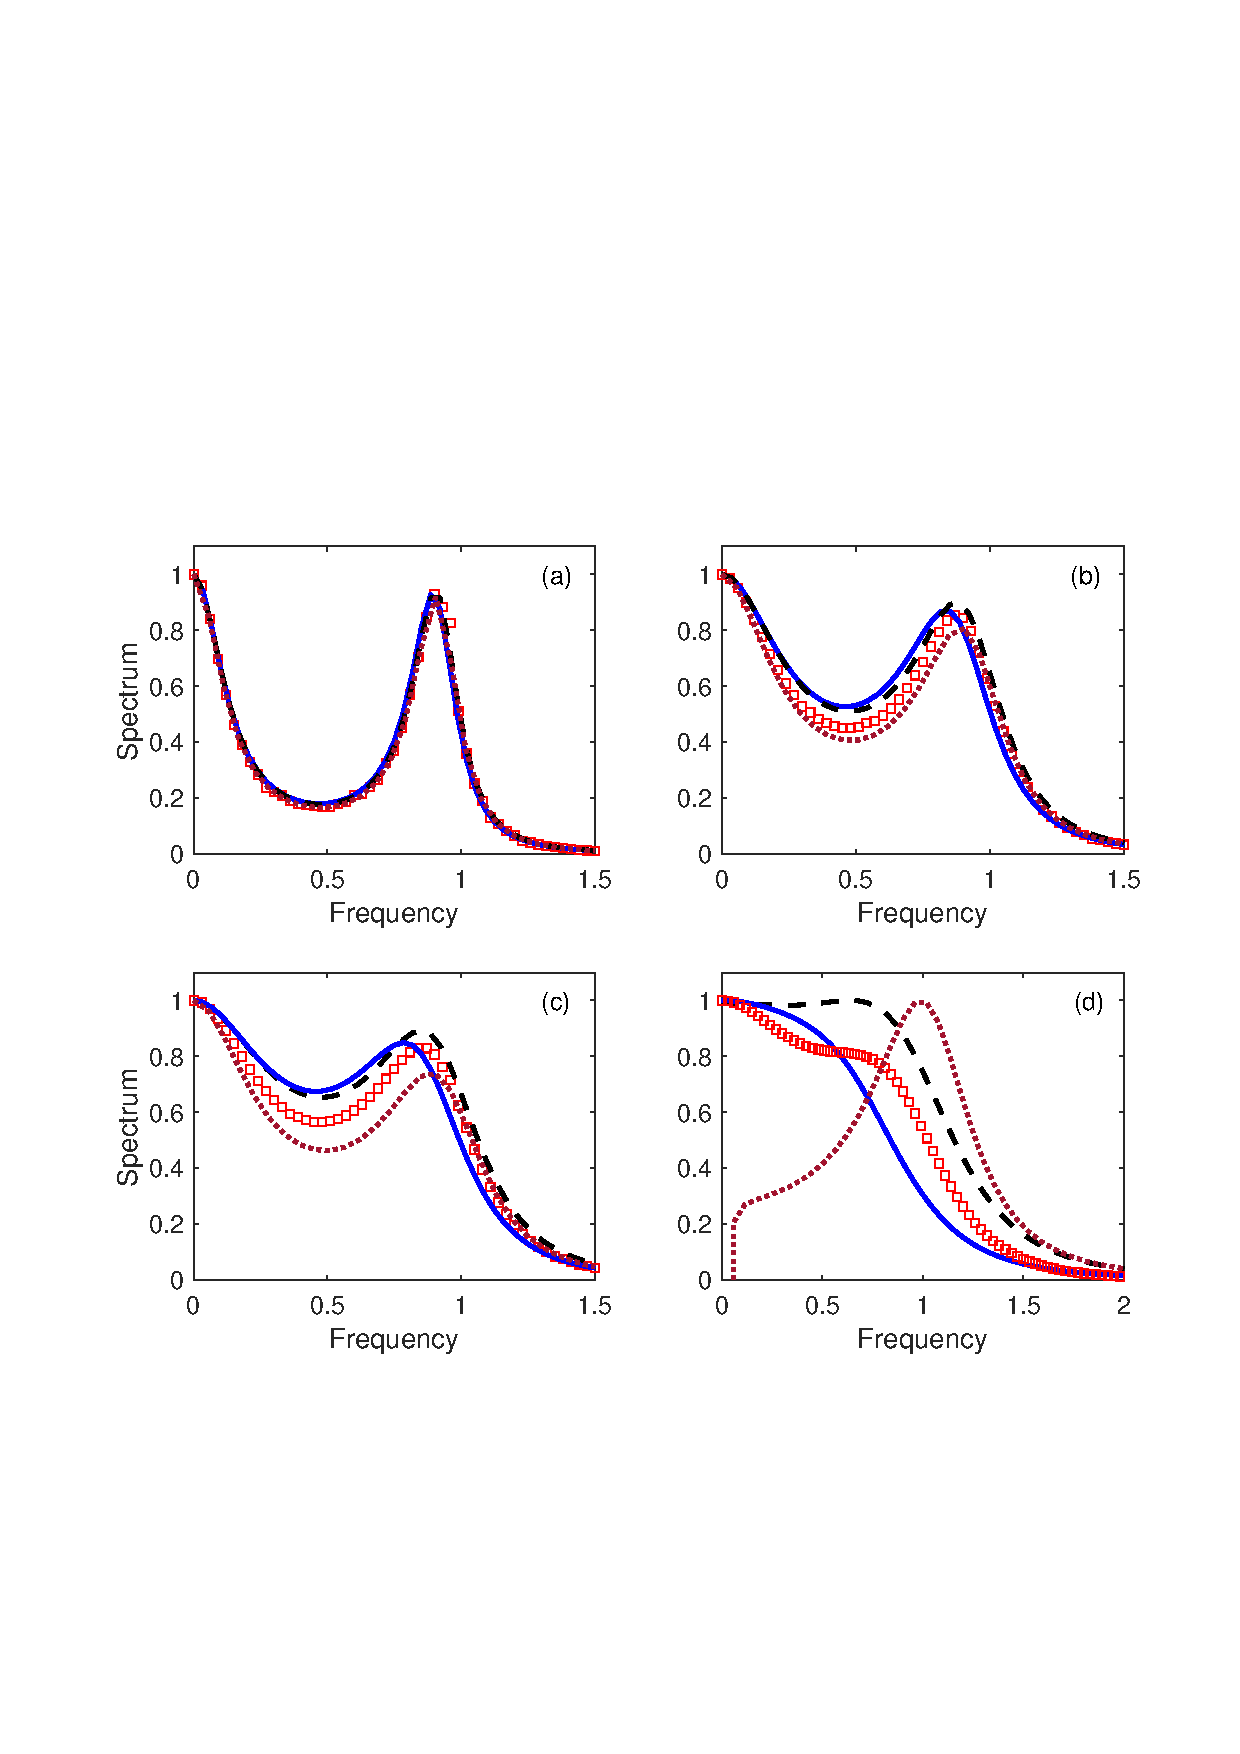
\includegraphics[width=0.7\textwidth]{FluidDynamic/IMG/s_NSBurnett.pdf}
	\caption{Spontaneous RBS spectra when (a) $\text{Kn}=0.02$, (b) $\text{Kn}=0.04$, (c) $\text{Kn}=0.05$, and (d) $\text{Kn}=0.1$. Solid, dashed and dotted lines are results from the NS, Burnett and super-Burnett equations, respectively.  } % In this and subsequent figures, squares represent results from the LBE for Maxwellian gases if without specification.
	\label{fig:NSBurnett}
\end{figure}	
% Burnett equation

If the Chapman-Enskog expansion is applied to the second-order of $\text{Kn}$, the Burnett equations can be derived. For Maxwellian molecules, the linearized constitutive relations for the stress and heat flux become
\begin{equation}
\begin{aligned}[b]
\sigma^{(B)}=\sigma^{(NS)}-\text{Kn}^2\left(\frac{4}{3}\frac{\partial^2 \rho}{\partial x^2}-\frac{2}{3}\frac{\partial^2 {T}}{\partial x^2}\right),\\
q^{(B)}=q^{(NS)}-\frac{7}{4}\text{Kn}^2\frac{\partial^2u}{\partial x^2}.
\end{aligned}
\end{equation}	
\index{Chapman-Enskog expansions!Burnett equation}
\index{Chapman-Enskog expansions!Super-Burnett equation}



The super-Burnett equations can be derived if the Chapman-Enskog expansion is applied to the third-order of $\text{Kn}$, where the stress and heat flux in this particular problem are~\cite{Shavaliyev1993}:
\begin{equation}\label{SB}
\begin{aligned}[b]
\sigma^{(SB)}=\sigma^{(B)}+\frac{2}{9}\text{Kn}^3\frac{\partial^3 u}{\partial x^3},\\
q^{(SB)}=q^{(B)}+\text{Kn}^3\left(\theta_7\frac{\partial^3T}{\partial x^3}-\frac{5}{8}\frac{\partial^3\rho}{\partial x^3}\right),
\end{aligned}
\end{equation}
with $\theta_7=-{157}/{16}$ for Maxwellian molecules. 


%Like the Burnett equations, the super-Burnett equations are  unstable to disturbance with small wavelength. Zhong \textit{et al.} proposed the augmented Burnett equations~\cite{Zhong1993}. They kept the nonlinear expressions for the stress and heat flux from the Burnett equations at the second order of $\text{Kn}$, while the third-order parts are chosen from the super-Burnett equations as the corresponding linearized terms in one-dimensional problem. In this Rayleigh-Brillouin scattering problem, expressions for the stress and heat flux in the augmented Burnett equations are also given by Eq.~\eqref{SB}. The coefficient $\theta_7$, however, is chosen as $\theta_7=11/16$, due to the wrong calculation in Ref.~\cite{WCS1982}; this erroneous parameter happens to make the augmented Burnett equations stable.


Figure~\ref{fig:NSBurnett} shows the spectra of spontaneous RBS. It is seen that the NSF equations perform well up to $\text{Kn}\approx0.02$. The Burnett equations, although accurate to the second-order of $\text{Kn}$, seems do not improve the accuracy in predicting the spectra of spontaneous RBS. It is surprising that the super-Burnett equations derived to the third-order of $\text{Kn}$ in the Chapman-Enskog expansion perform much worse than the Burnett equations that are obtained from the Chapman-Enskog expansion to the second-order of $\text{Kn}$, especially when $\text{Kn}=0.1$. This conforms the criticism that one does not know what step of the approximation is required or sufficient to obtain a solution that is correct up to order $\text{Kn}^n$~\cite{Cercignanibook1988,Sone2002Book}. 




\subsubsection{Moment equations}
\index{moment equations}
\index{moment equations!Grad 13}

%Moment equations are derived through the method of ansatz, that is, the VDF $f(t,\bm{x},\bm{v})$ in the Boltzmann equation is assumed to be the product of Gaussian function and several low-order Hermite polynomials with the coefficients related to the moments of VDF. 

%The first set of moment equations obtained by Grad~\cite{Grad1949} consists of 13 macroscopic quantities, where the distribution function is given by Eq.~\eqref{Grad13VDF}. 

In Rayleigh-Brillouin scattering the stress and heat flux in the G13 equations satisfy the following equations:
\begin{equation}\label{G13}
\begin{aligned}[b]
\frac{\partial \sigma}{\partial t}+\frac{4}{3}\frac{\partial u}{\partial x}+\frac{8}{15}\frac{\partial q}{\partial x}=-\frac{\sigma}{\text{Kn}},\\
\frac{\partial q}{\partial t}+\frac{\partial \sigma}{\partial x}+\frac{5}{2}\frac{\partial {T}}{\partial x}=-\frac{2}{3}\frac{q}{\text{Kn}}.
\end{aligned}
\end{equation}

The spectrum of spontaneous RBS can be obtained by solving the following matrix:
\begin{equation}\label{Grad_sp}
\left[ \begin {array}{cccccc} 
-i\varpi&2i\pi&0 &0 &0
\\ \noalign{\medskip}
2i\pi&-i\varpi &2i\pi &2i\pi &0
\\ \noalign{\medskip}
0&2\,i\pi&-\frac{3}{2}i\varpi &0 &2i\pi
\\ \noalign{\medskip}
0  &\frac{8}{3}i\pi  & 0 &-i\varpi+\frac{1}{\text{Kn}}  &\frac{16}{15}i\pi
\\ \noalign{\medskip}
0  & 0 & 5i\varpi &2i\varpi  &-i\varpi+\frac{2}{3\text{Kn}}
\end {array} \right]
\left[ \begin {array}{cccccc} \hat\rho \\ \hat{u}
\\ \hat{T}  \\ \hat\sigma \\ \hat{q}
\end {array} \right] =
\left[ \begin {array}{cccc} 1\\ 0
\\ 0 \\0 \\0
\end {array} \right], 
\end{equation}	
where $\hat{\sigma}$ and $\hat{q}$ are respectively the Laplace-Fourier transform of $\sigma$ and $q$ in the temporal-spatial domains.
%where the analytical solutions are too complicated and hence are not shown.

%\begin{figure}
%	\centering
%	\includegraphics[scale=0.55,viewport=80 20 740 370,clip=true]{Moment2.eps}
%	\caption{Spectra of the spontaneous (top row) and coherent (bottom row) RBS. The horizontal and vertical axis are the normalized frequency and spectrum, respectively. Form the left to right, the Knudsen number in each column are 0.04, 0.06, 0.08, and 0.1, respectively. Solid, dashed, and dotted lines are the results from the G13, R13, and R26 moment equations, respectively. Triangles and solid circles are results from Eu's generalized hydrodynamic equations and coupled constitutive relations~\eqref{CCR}, respectively.  }
%	\label{fig:moment}
%\end{figure}


\begin{figure}[t]
	\centering
	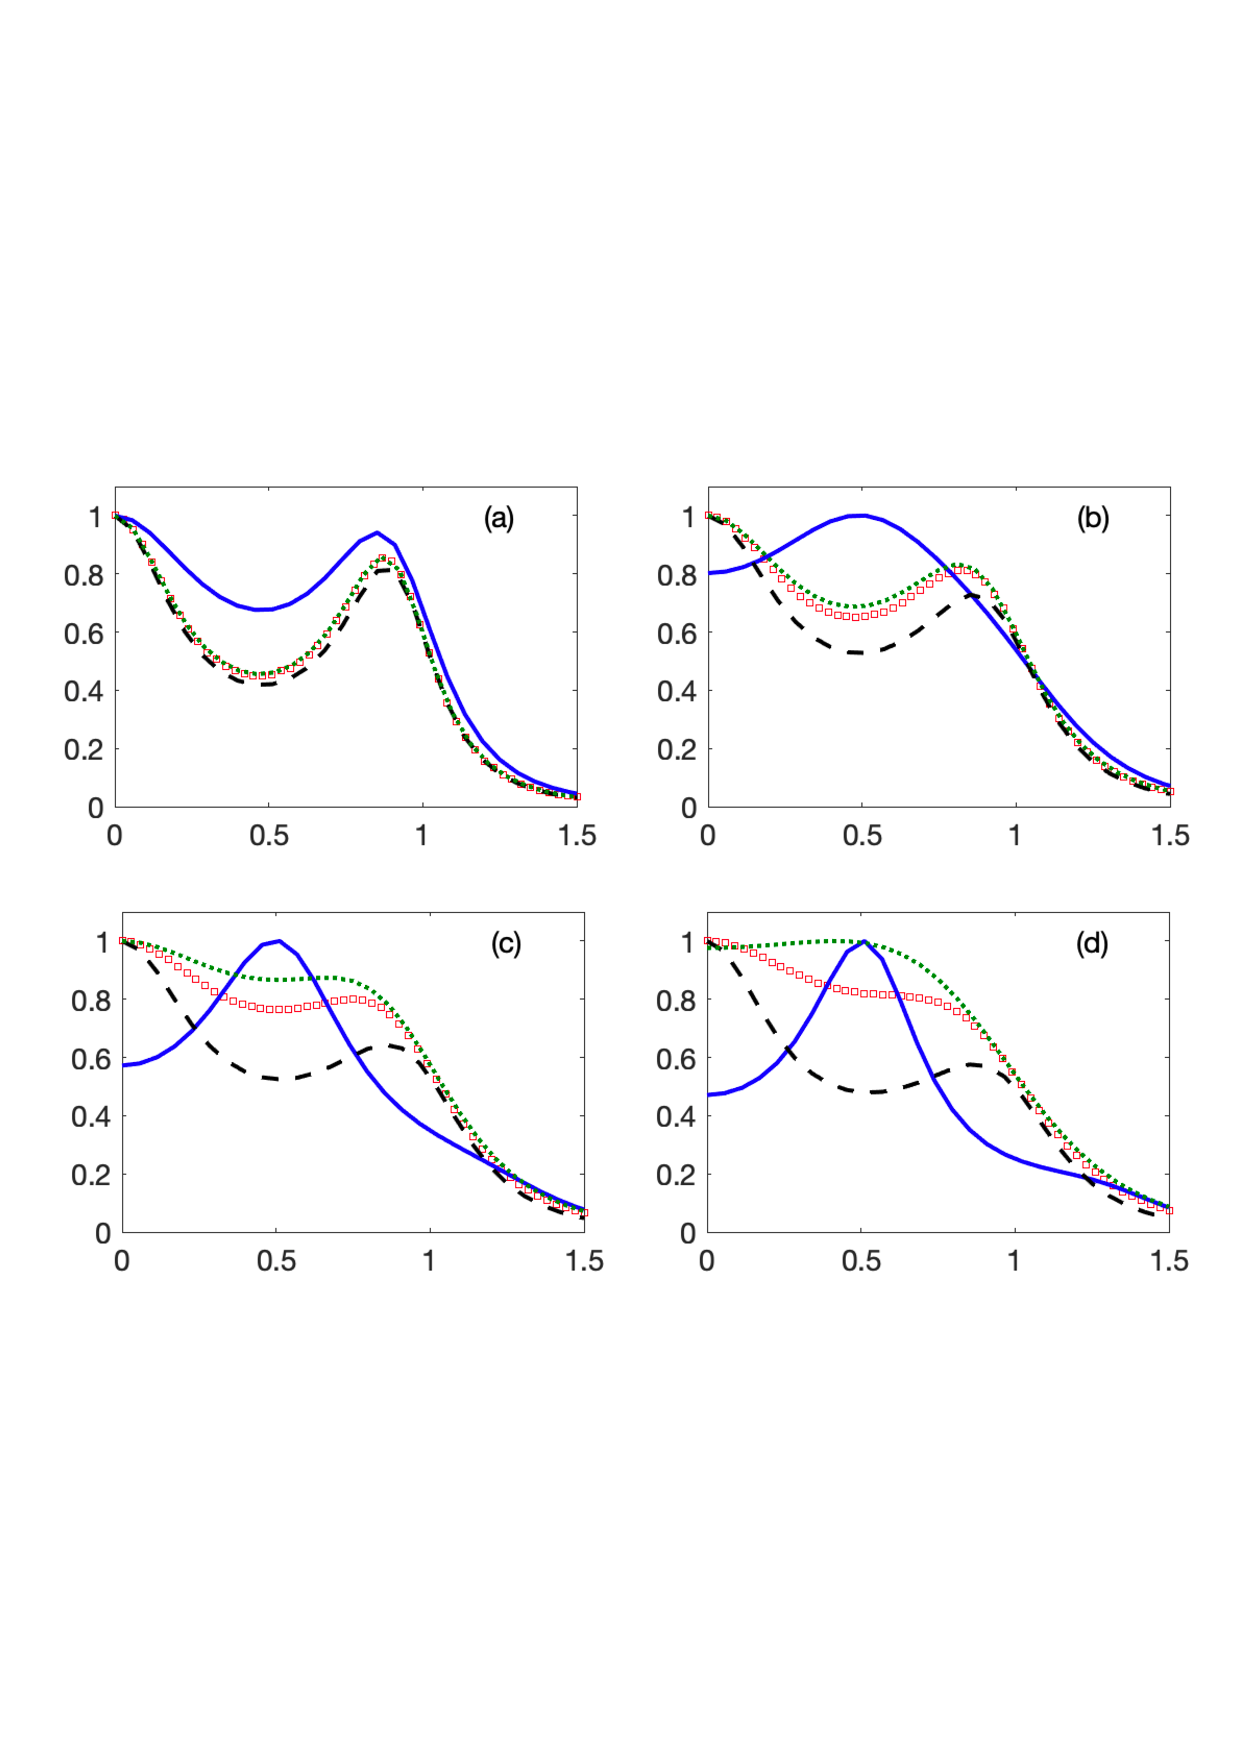
\includegraphics[scale=0.6]{FluidDynamic/IMG/Moment.pdf}
	\caption{Spectra of the spontaneous RBS. The horizontal and vertical axis are the normalized frequency and spectrum, respectively. Form the left to right, the Knudsen numbers in each column are 0.04, 0.06, 0.08, and 0.1, respectively. Solid, dashed, and dotted lines are the results from the G13, R13, and R26 moment equations, respectively.  }
	\label{fig:moment}
\end{figure}


\index{moment equations!Regularized 13}

Note that the G13 equations are accurate to the second-order of $\text{Kn}$, which have been extended to the R13 equations that are accurate to the third-order of $\text{Kn}$~\cite{henning}. The governing equations for the stress and heat flux become
\begin{equation}
\begin{aligned}[b]
\frac{\partial \sigma}{\partial t}+\frac{4}{3}\frac{\partial u}{\partial x}+\frac{8}{15}\frac{\partial q}{\partial x}-\frac{6}{5}\text{Kn}\frac{\partial^2\sigma}{\partial x^2}=-\frac{\sigma}{\text{Kn}},\\
\frac{\partial q}{\partial t}+\frac{\partial \sigma}{\partial x}+\frac{5}{2}\frac{\partial {T}}{\partial x}-\frac{18}{5}\text{Kn}\frac{\partial^2q}{\partial x^2}=-\frac{2}{3}\frac{q}{\text{Kn}}.
\end{aligned}
\end{equation}


Similarly, the evolution of the stress and heat flux in the linearized R26 equations, which are accurate up to the fifth-order of $\text{Kn}$, are governed by~\cite{Gu2009JFM}:
\begin{equation}
\begin{aligned}[b]
\frac{\partial \sigma}{\partial t}+\frac{4}{3}\frac{\partial u}{\partial x}+\frac{8}{15}\frac{\partial q}{\partial x}+\frac{\partial \bar{m}}{\partial x}=-\frac{\sigma}{\text{Kn}},\\
\frac{\partial q}{\partial t}+\frac{5}{2}\frac{\partial {T}}{\partial x}+\frac{\partial \sigma}{\partial x}+\frac{1}{6}\frac{\partial\bar{\Delta}}{\partial{}x}+\frac{1}{2}\frac{\partial\bar{R}}{\partial{x}}=-\frac{2}{3}\frac{q}{\text{Kn}},
\end{aligned}
\end{equation}
where the higher-order moments $\bar{m}$, $\bar{\Delta}$, and $\bar{R}$ are governed by the following equations:
\begin{equation}\label{Gu_R26}
\begin{aligned}[b]
\frac{\partial\bar{m}}{\partial{t}}+\frac{9}{5}\frac{\partial\sigma}{\partial{x}}+\frac{9}{35}\frac{\partial\bar{R}}{\partial{x}}-\frac{16}{7}\frac{\text{Kn}}{A_{\phi1}}\frac{\partial^2\bar{m}}{\partial{x}^2}=-\frac{3}{2}\frac{\bar{m}}{\text{Kn}},\\
\frac{\partial\bar{\Delta}}{\partial{t}}+8\frac{\partial{q}}{\partial{x}}-\frac{7\text{Kn}}{3}\frac{\partial^2\bar{\Delta}}{\partial{x}^2}-4\text{Kn}\frac{\partial^2\bar{R}}{\partial{x^2}}=-\frac{2}{3}\frac{\bar{\Delta}}{\text{Kn}},\\
\frac{\partial\bar{R}}{\partial{t}}+\frac{56}{15}\frac{\partial{q}}{\partial{x}}+2\frac{\partial\bar{m}}{\partial{x}}-\frac{\text{Kn}}{5}\left(\frac{54}{7A_{\psi1}}+\frac{16}{3}\right)\frac{\partial^2\bar{R}}{\partial{x}^2}-\frac{28\text{Kn}}{45}\frac{\partial^2\bar{\Delta}}{\partial{x}^2}=-\frac{7}{6}\frac{\bar{R}}{\text{Kn}},
\end{aligned}
\end{equation}
with $A_{\phi1}=2.097$ and $A_{\psi1}=1.698$.

\index{moment equations!Regularized 26}

Figure~\ref{fig:moment} shows the RBS spectra obtained from the G13, R13, and R26 moment equations. When $\text{Kn}=0.02$, all the moment equations predict the same spectrum as that from the LBE. However, even when $\text{Kn}$ is increased to $\text{Kn}=0.04$, spectra predicted by the G13 equations deviate significantly from those of the LBE. The R13 equations are accurate up to $\text{Kn}\approx0.04$, while the R26 equations are accurate up to $\text{Kn}\approx0.06$. 

%Interestingly,  we accidentally changed the value of $A_{\psi1}$ to $-1.698$, and found that excellent agreement is achieved for Knudsen number up to $0.1$ for both spontaneous and coherent RBS.

%Overall, the accuracy of the R26  equations are worse than the augmented Burnett equation with $\theta_7=-60/16$. 

%It should be noted that Gu has also derived the regularized 35 moment equations, where the distribution function is expanded to the fifth-order polynomials and all the relevant moments are included. For the 1D Rayleigh-Brillouin scattering problem, only one extra equation for the higher-order moment is added:
%\begin{equation}
%\frac{\partial \bar\phi}{\partial{t}}+\frac{16}{7}\frac{\partial \bar{m}}{\partial{x}}-\frac{96\text{Kn}}{245A_{\psi1}}\frac{\partial^2 \bar{R}}{\partial{x}^2}-\frac{25\text{Kn}}{9A_{w1}}\frac{\partial^2\bar\phi}{\partial{x}^2}=-\frac{A_{\phi1}}{\text{Kn}}\bar{\phi},
%\end{equation}
%with $A_{w1}=2.743$ for Maxwellian molecules, while the equation for $\bar{m}$ in~\eqref{Gu_R26} is replaced by
%\begin{equation}
%\frac{\partial\bar{m}}{\partial{t}}+\frac{9}{5}\frac{\partial\sigma}{\partial{x}}+\frac{9}{35}\frac{\partial\bar{R}}{\partial{x}}+\frac{\partial\bar{\phi}}{\partial{x}}=-\frac{3}{2}\frac{\bar{m}}{\text{Kn}}.
%\end{equation}
%It is noted by Gu that from 1D shear flow the R35 equations are better than the R26 equations, but not much. The same conclusion can be made in the Rayleigh-Brillouin scattering problem, where the spectra from the R26 and R35 equations are nearly identical, since there are both accurate to $O(\text{Kn}^5)$. In 2D or 3D situations, the computational costs increase as more equations are included in the system, but the accuracy is not gained proportionally. Therefore, the R26 moment equations are recommended. 






%\subsection{Rational extended thermodynamics}
%
%\begin{figure}
%	\centering
%	\includegraphics[scale=0.5,viewport=0 0 660 290,clip=true]{PRL.eps}
%	\caption{Comparisons in the spectra of spontaneous RBS between the experimental data (the solid line) by Greytak \& Benedek~\cite{Greytak1966PRL}, the LBE (the dashed line) for polyatomic gas~\cite{Wu2015JFM}, and the rational extended thermodynamics with 14 moments (the dash-dotted line) by Ruggeri \& Sugiyama~\cite{Ruggeri2015Book}. The light is scattered from CO$_2$ when $\text{Kn}=0.1114$. Note that the frequency is normalized by 1.06~GHz, and the shown spectra are the convolution of $S_s(Kn,f_s)$ and the Lorentzian function $Lor(f_s)$ with the Full Width at Half Maximum being 210~MHz, i.e.,  $Lor(f_s)\propto1/(f_s^2+9.8\times10^{-3})$.   }
%	\label{fig:PRL}
%\end{figure}
%
%
%
%Rational extended thermodynamic equations for rarefied gas dynamics are derived from the gas kinetic equation in a manner similar to the derivation of moment equations, but the distribution function is instead obtained by the maximum entropy principle. Recently, it has been used to study the spontaneous RBS spectra in polyatomic gases by considering only 14 moments (i.e. in addition to the 13 moments in the G13 equations, the dynamical pressure that is related to the bulk viscosity is also considered); the corresponding macroscopic equations can be found in the Chapter 9 of the book by Ruggeri \& Sugiyama~\cite{Ruggeri2015Book}, which degenerate to the G13 equations for monatomic gases when the deviation from equilibrium is weak. 
%
%
%The spectrum of spontaneous RBS from the rational extended thermodynamics with 14 moments has been compared with the experiment~\cite{Greytak1966PRL}, where the light with the effective wave vector $k=1.98\times10^{5}$~cm$^{-1}$ is scattered by CO$_2$ at a temperature 298~K and pressure 750~mm~Hg. In the numerical calculation of the spectrum of spontaneous RBS based on the LBE for polyatomic gas, we use the method developed in Ref.~\cite{Wu2015JFM}, with the ratio of the bulk viscosity to the shear viscosity of CO$_2$ being 0.39~\cite{Gu2014OL}. From Fig.~\eqref{fig:PRL} we can find the huge difference between the results of rational extended thermodynamics and experiment, while our LBE solution gives a good prediction of the RBS spectrum. We conclude that the accuracy of the rational extended thermodynamics is roughly at the same order with the G13 equations.



\subsubsection{Discussions}\label{Conclusions}

%The accuracy of macroscopic equations is summarized and visualized more clearly in %Fig.~\ref{fig:compare}, where the relative difference in the RBS spectra is shown as a function of the Knudsen number. The solution may be viewed being accurate when the relative difference is less than 0.05. It should be noted that in Rayleigh-Brillouin scattering both the spatial and temporal Knudsen numbers play important roles. For steady-state problems, the range of applicability of these macroscopic equations may move to larger values of $\text{Kn}$.  

Based on the benchmarking solutions from the Boltzmann equation for the spectra of Rayleigh-Brillouin scattering, we have assessed the accuracy of macroscopic equations. Interestingly, as the order of Chapman-Enskog expansion increases, the accuracy of the obtained macroscopic equations does not necessarily increase (say, when $\text{Kn}\gtrapprox0.03$, the super-Burnett equations are less accurate than the Burnett equations), which confirms the criticism that one does not know what step of the approximation is required or sufficient to obtain a solution that is correct up to order $\text{Kn}^n$. For the (regularized) moment equations, however, the accuracy in the prediction of RBS spectra is consistent with the accuracy in deriving these equations, that is, increases monotonically from the G13, R13, to the R26 moment equations. 

%
%\begin{figure}[t]
%	\centering
%	\includegraphics[scale=0.5]{relative_srbs}
%	\caption{
%		(left) Difference $\int_{\infty}^{\infty} |S^{LBE}-S^{Mac}| df_s$ in the spectrum of spontaneous RBS between solutions of the LBE and macroscopic equations. Note that before the comparison, areas of RBS spectra are normalized to unity. The solution may be viewed to be accurate when the relative difference is less than 0.05. 
%	}
%	\label{fig:compare}
%\end{figure}


%The Eu's generalized hydrodynamic equations, where the VDF contains the fourth-order Hermite polynomial, has the same level accuracy as the G13 equations, where the distribution function is expanded only up to the third-order Hermite polynomial, and it is less accurate than the R13 equations. The Brenner's bi-velocity fluid model and Dadzie's thermo-mechanically consistent Burnett equations, which contain free parameters that can not be determined from fundamental physical laws, both involve the concept of volume diffusion, do not perform well compared to the R13 equations, even when the best parameters are selected.  

\begin{figure}[t]
	\centering
	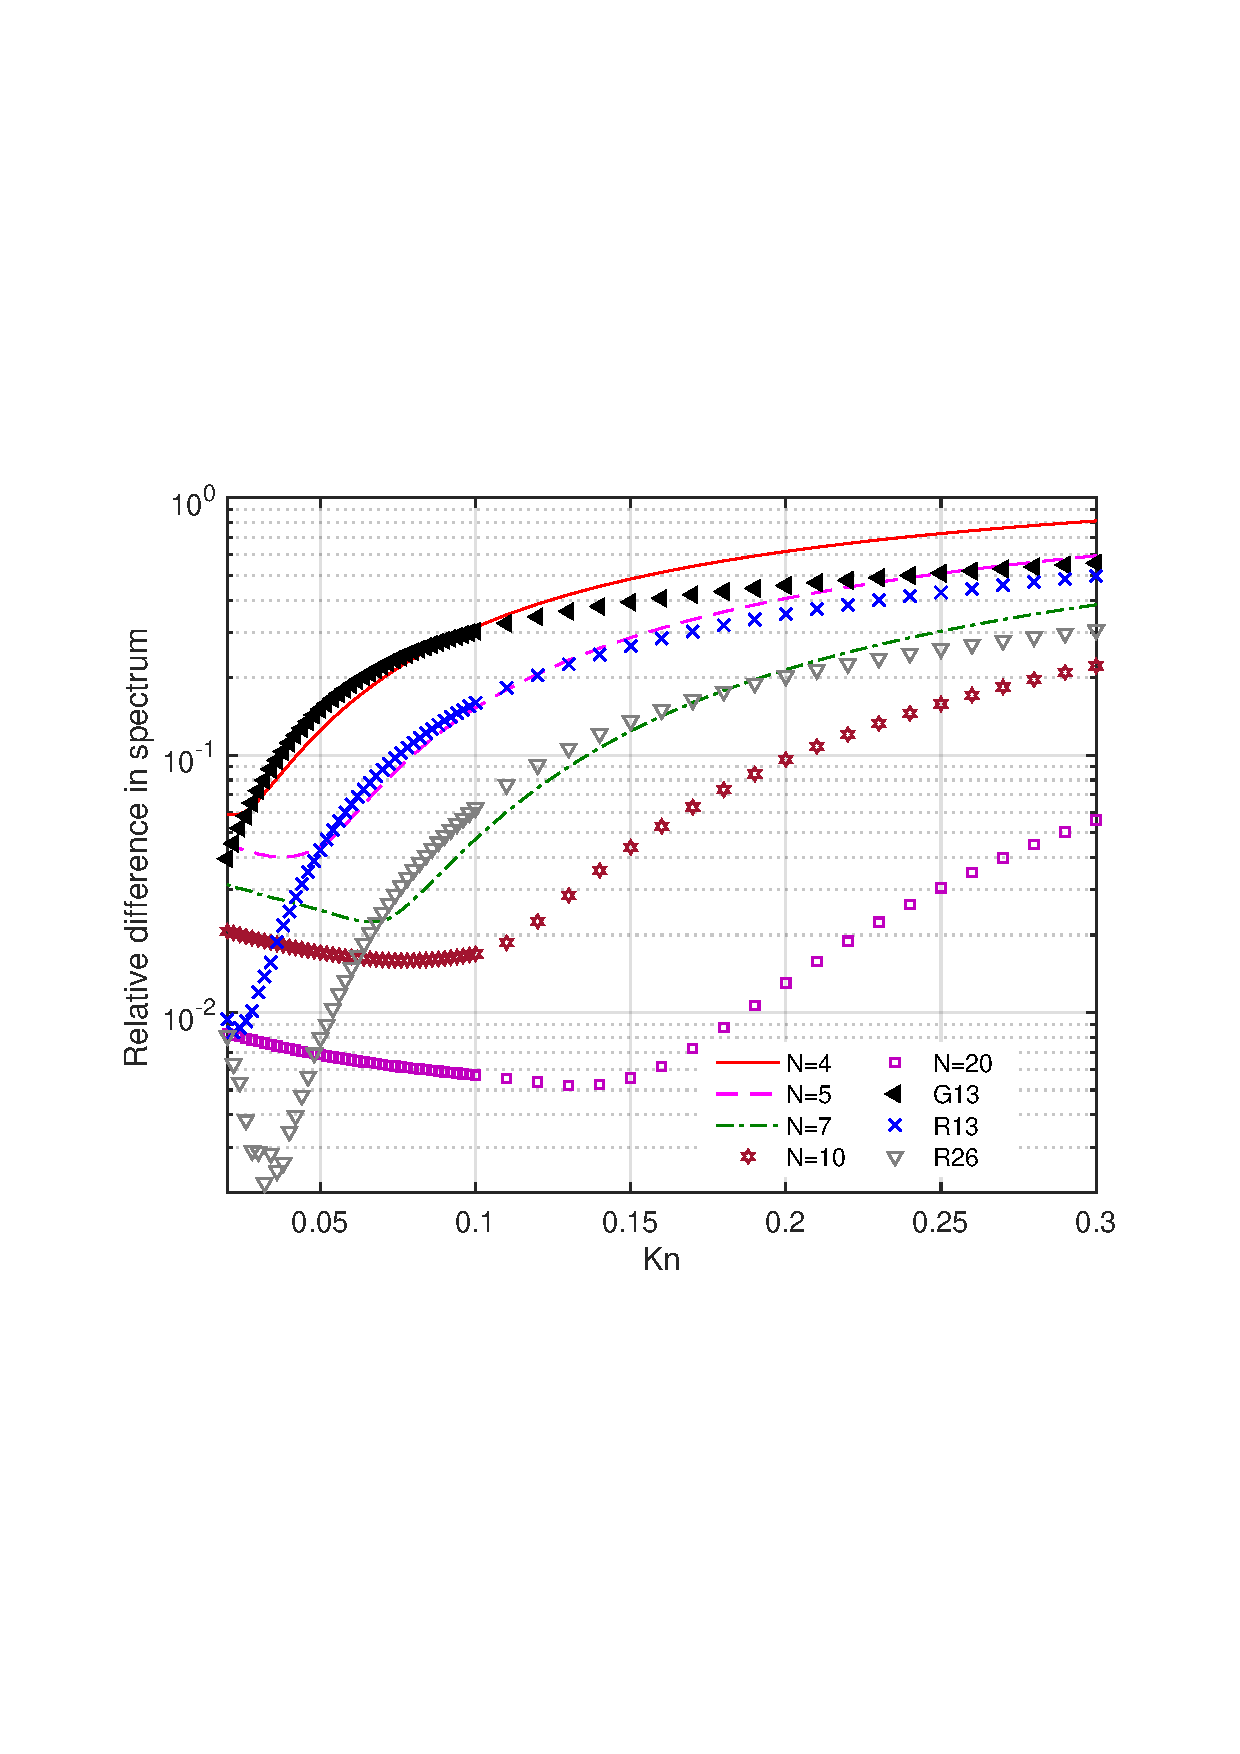
\includegraphics[scale=0.6]{FluidDynamic/IMG/compare_GH.pdf}
	\caption{Difference $\int_{\infty}^{\infty} |S^{LBE}-S_{GH}^{N}| df_s$ in the spectrum of spontaneous RBS, where $S_{GH}^{N}$ is the spectrum obtained by solving the Shakhov kinetic model in section~\ref{shakhov_model_chapter} with the Gauss-Hermite quadrature of order $N$.  Note that before the comparison, areas of RBS spectra are normalized to unity. The solution may be viewed being accurate when the relative difference is less than 0.05. Also note that the relative difference when $N=5, 7, 10$ and 20 does not decrease with $\text{Kn}$ when $\text{Kn}\lesssim0.1$ is probably because the spectrum between the Rayleigh and Brillouin peaks is nearly zero [see Fig.~\ref{fig:RBS_demo}] so any tiny difference is magnified.}
	\label{fig:compare2}
	% in the three-dimensional molecular velocity space $\bm{v}$, the number of total discrete velocity points is $N^3$; note that the corresponding Grad moment equations have $(N+1)(N+2)(N+3)/6$ moments~\cite{FanThesis}.
\end{figure}

From these comparisons, it may be concluded that the regularized moment method is a proper way to derive higher-order macroscopic equations to describe the rarefied gas dynamics, where the derivation is straightforward, and its accuracy is definitive and controllable, that is, the accuracy increases with the number of moments or order of Hermite polynomials used to approximate the VDF. This is quite important in numerical simulations, where the error may be estimated in prior. To further illustrate this point, we study the performance of higher-order moment method, by solving the linearized Shakhov equation numerically using the discrete velocity method based on the Gauss-Hermite quadrature~\cite{Shakhov_S}, which is equivalent to the Grad moment method at different order of approximations~\cite{Shan2006JFM}. To be specific, if the $N$-th order Gauss-Hermite quadrature is considered in the discretization of molecular velocity space, the moment up to the order $N-1$ can be captured accurately~\cite{Shan2006JFM}. Consider the fact that the G13 equations where the distribution function is expanded up to third-order Hermite polynomials are accurate to $O(\text{Kn}^2)$, the numerical solution of the Shakhov equation based on the Gauss-Hermite quadrature of order $N$ has an accuracy of $O(\text{Kn}^{N-2})$.






%\cite{Shakhov1968,Shakhov_S,Shakhov1974}:
%\begin{equation}\label{Shakhov_RBS}
%\begin{aligned}[b]
%\frac{\partial h}{\partial t}+v_1\frac{\partial h}{\partial x_1}=\frac{\delta_{rp}}{\pi^{3/2}}\exp(-v^2)
%\left[\varrho+2u_1v_1+T\left(v^2-\frac{3}{2}\right)+\frac{4}{15}q_1v_1\left(v^2-\frac{5}{2}\right)\right]
%-\delta_{rp}h,
%\end{aligned}
%\end{equation}
%where
%$\varrho=\int{h}\mathrm{d}\bm{v}$ is the perturbed number density, $u_1=\int v_1{h}\mathrm{d}\bm{v}$ is the perturbed velocity,  $T=\frac{2}{3}\int{}v^2{h}\mathrm{d}\bm{v}-\rho$ is the perturbed temperature, and $q_1=\int{}v^2v_1{h}\mathrm{d}\bm{v}-\frac{5}{2}u_1$ is the perturbed heat flux. 







Using solutions of the Shakhov model approximated by the 60th-order Gauss-Hermite quadrature as reference, we analyze the accuracy of various orders of moment equations in Fig.~\ref{fig:compare2}. We also show the relative error in the spectrum from comparisons between the G13/R13/R26 equations and the LBE. Obviously, as more moments (i.e., higher-order quadrature) are included, the accuracy increases monotonically. When $N=4$, the Gauss-Hermite quadrature yields an equivalent moment system accurate to $O(\text{Kn}^2)$, therefore, the relative difference curve almost overlaps that from the G13 equations. Similarly, $N=5$ and 7 yield equivalent moment systems accurate to $O(\text{Kn}^3)$ and $O(\text{Kn}^5)$, respectively. Therefore, relative difference curves nearly overlap with those from the R13 and R26 moment equations in a wide range of Knudsen numbers.


It can also be seen from Fig.~\ref{fig:compare2} that at large values of $\text{Kn}$ the convergence rate of moment equations is slow. For example, when $\text{Kn}=0.3$, when $N$ is increased from 5 to 20, that is, when the accuracy of the equivalent moment systems is increased from $O(\text{Kn}^3)$ to $O(\text{Kn}^{18})$, the error is only reduced by about one order of magnitude. And the solution of $N=20$ can be marginally viewed as accurate. Accuracy of moment systems may become worse in wall-bounded problems such as the Poiseuille flow between two parallel plates~\cite{Su2007PRE}, as Gauss-Hermite polynomials are not good at capturing the discontinuities in VDF. 


To conclude, higher-order Chapman-Enskog expansion does not necessarily lead to more accurate prediction of rarefied gas dynamics, while the moment method produces more accurate results when more moments are included, but the convergence to true solutions may be slow when the Knudsen number is large. 

%This research would shed some light on how to choose/develop macroscopic equations for rarefied gas dynamics. % After all, knowing history helps advance future without past mistakes.      









\section{Convergence speed of moment equations}\label{sound_section}
\index{sound wave}

We now assess the accuracy of macroscopic equations in the problem of sound propagation in gas confined between the transducer and receiver~\cite{Wu2020AIA}, see Fig.~\ref{fig:sound}. We use the linearized Shakhov kinetic model equation, as the Gauss-Hermite quadrature can be applied~\citep{Shan2006JFM} to mimic the behavior of moment equations at any order, replacing the complicated derivation and solving of high-order moment equations beyond R26; the numerical method is given in Section~\ref{sound_gsis_1D}, where the numerical solution agrees well with  experimental data of Schotter~\cite{Schotter1974}, see Fig.~\ref{fig:sound}.


Macroscopic equations are the same as in the Rayleigh-Brillouin scattering problem, except for the R26 equations we have $A_M=1=A_{\Delta1}=A_{\Omega1}=A_{\phi1}=A_{\psi1}=A_{R1}=1$ in Eq.~\eqref{Gu_R26}, as derived from the Shakhov kinetic model. The boundary conditions for NS and R13 equations corresponding to the diffuse boundary condition for gas kinetic model equations can be found in Ref.~\cite{Struchtrup2011}, while that for R26 equations is given in Ref.~\cite{Gu2009JFM}.



\begin{figure}[t]
	\centering
	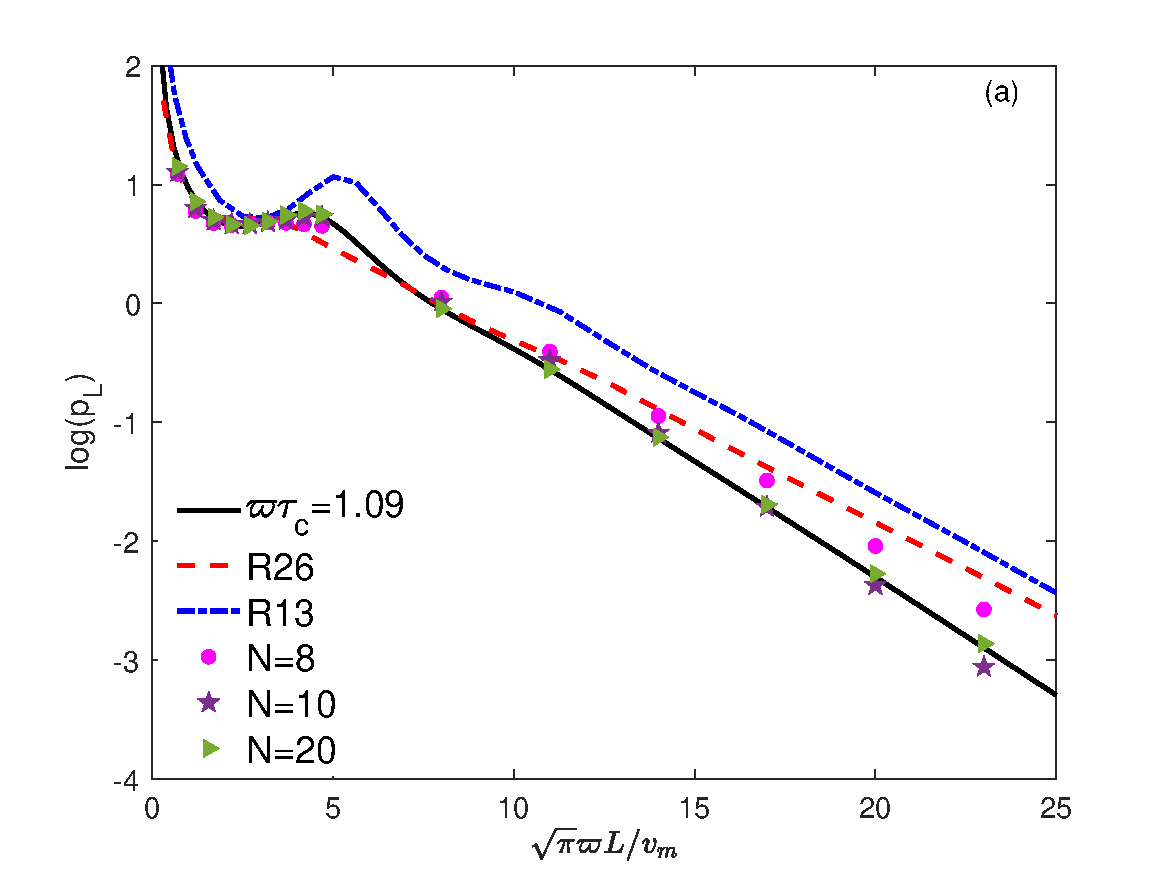
\includegraphics[width=0.49\textwidth]{FluidDynamic/IMG/testOmgTau1_09Copy.pdf}
	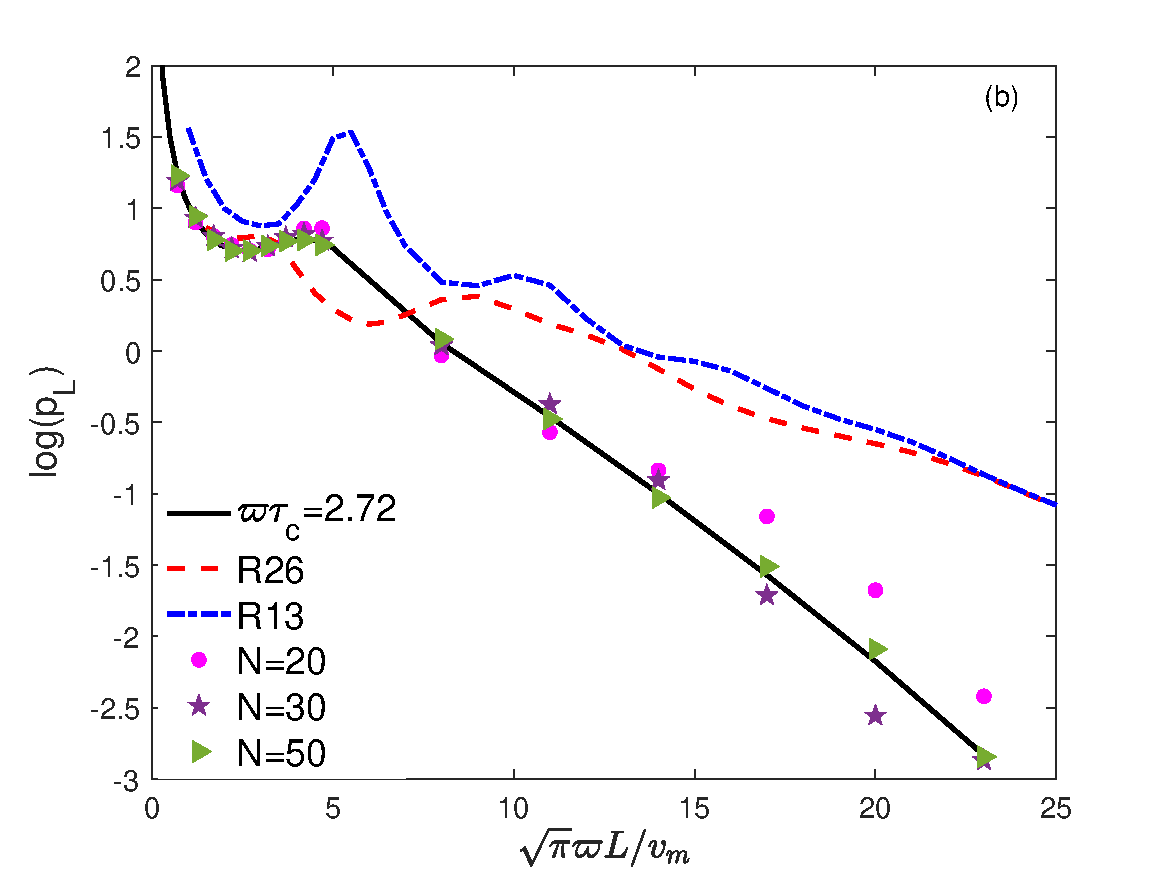
\includegraphics[width=0.49\textwidth]{FluidDynamic/IMG/testOmgTau2_72.pdf} 
	\caption{ Convergence test of moment equations: sound amplitude at the receiver as function of the dimensionless length $\sqrt\pi\varpi{L}/v_m$. Solid lines represent the accurate results from the Shakhov model solved by the discrete velocity method~\citep{SuArXiv2019}. Symbols are approximate solutions of the Shakhov model when the molecular velocity space $\bm{v}$ is discretized according to Gauss-Hermite quadrature of order $N$; these solutions are equivalent to those of Grad moment equations (having $(N+1)(N+2)(N+3)/6$ moments) that are accurate up to the order of $\text{Kn}^{N-2}$.  }
	\label{fig:sound_convergence}
\end{figure}


The parameter $\varpi{\tau_c}$ in Fig.~\ref{fig:sound} is proportional to the temporal Knudsen number $\text{Kn}_t$ as $\varpi{\tau_c}=2\sqrt{2}\pi\text{Kn}_t$. Therefore, as $\varpi{\tau_c}$ increases, the rarefaction effects become stronger, so macroscopic equations gradually lose accuracy. The NSF equations are accurate when $\varpi{\tau_c}=0.1$ (not shown), but are already very inaccurate when $\varpi{\tau_c}=0.3$; R13 equations, which are accurate to the order of $\text{Kn}^3$, give reasonable good results up to $\varpi{\tau_c}=0.3$, see  Fig.~\ref{fig:sound}. While R26 equations, which are accurate to the order of $\text{Kn}^5$, predict the normal pressure at the receiver fairly well up to $\varpi\tau_c=0.67$. This finding is in agreement with that in the spontaneous RBS, i.e., the accuracy of moment equations increases when more moments are included in macroscopic equations.  





%\subsubsection{Reason of slow convergence of moment systems}
%\index{Slow convergence}
\index{moment equations}

Now we consider the speed of convergence of moment systems for moderate and highly rarefied gas flows, that is, we are interested in how many moments should be included to give reasonable prediction of sound pressure. %Since the derivation and solving of higher-order moment system is extremely difficult, we solve the Shakhov model using the Gauss-Hermite quadrature of order $N$ instead; this is equivalent to the Grad moment equations where the VDF is expanded by Hermite polynomials up to $N$-th order. 



\index{velocity distribution function}
\begin{figure}[t]
	\centering
	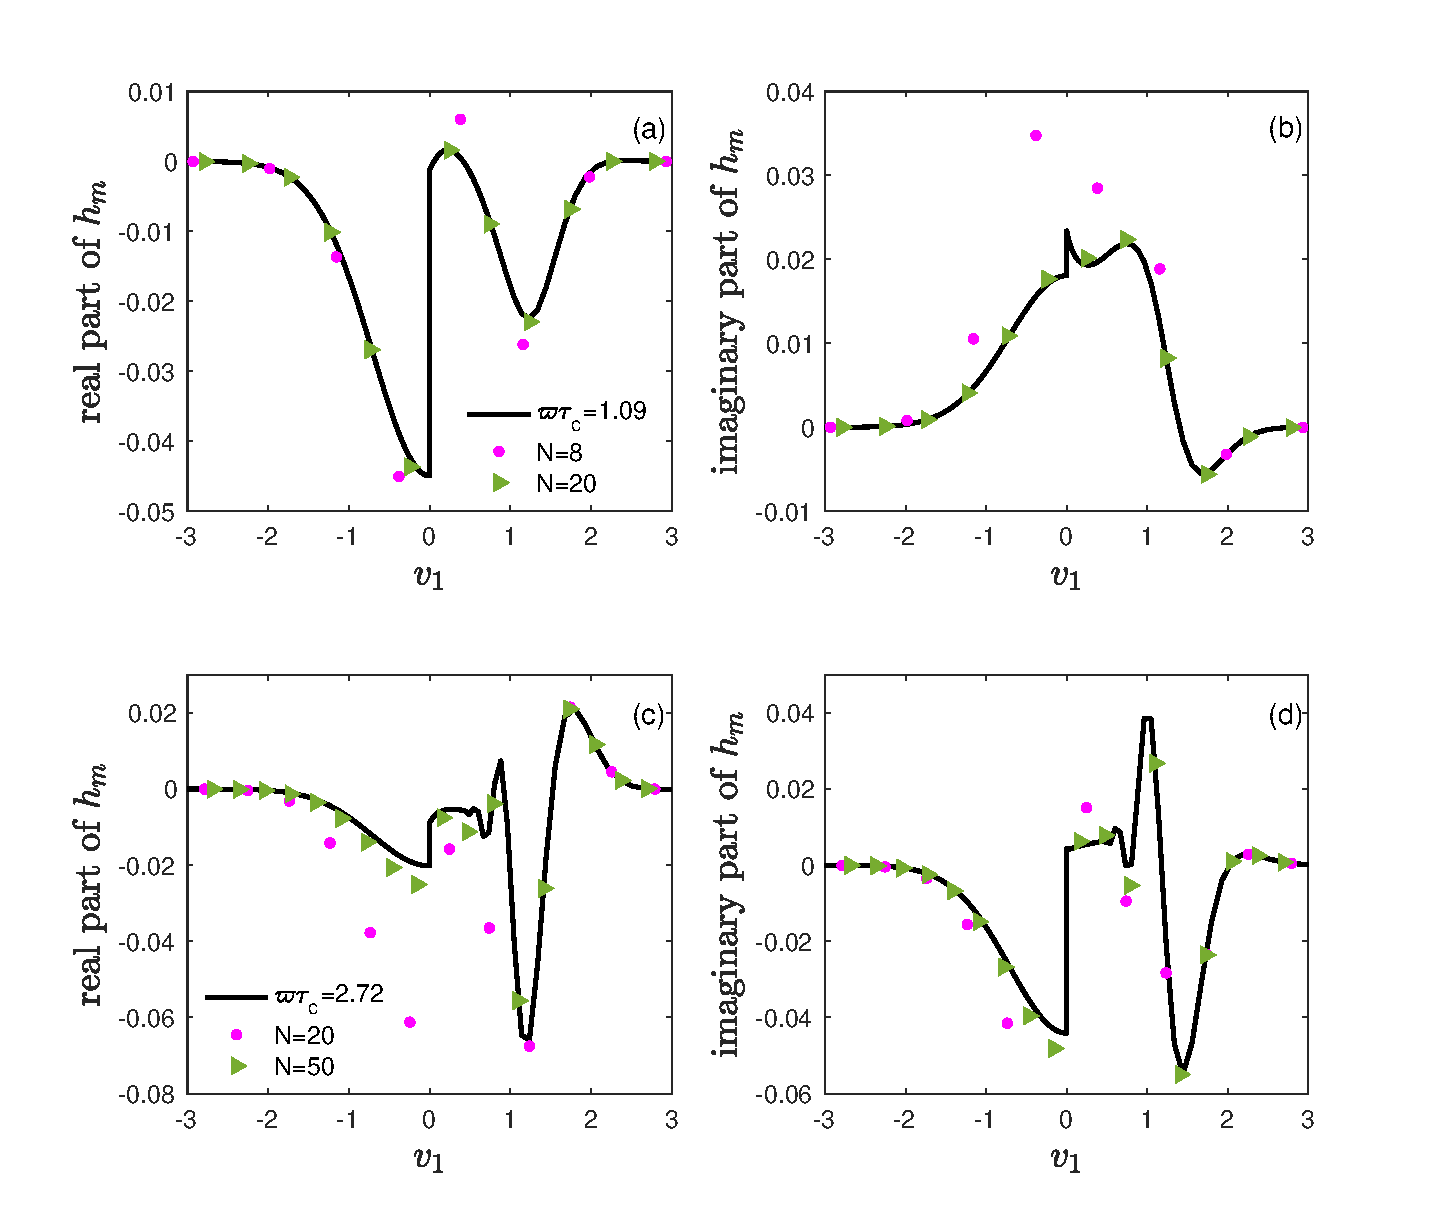
\includegraphics[width=0.8\textwidth]{FluidDynamic/IMG/vdf_sound.pdf}
	\caption{\index{velocity distribution function!marginal} Marginal VDF at the receiver. (a, b) $\varpi{\tau_c}=1.09$ and (c,d) $\varpi{\tau_c}=2.72$. In both cases, $\sqrt{\pi}\varpi{L}/v_m=20$. Solid lines represent the accurate results from the Shakhov model solved by the discrete velocity method~\citep{SuArXiv2019}, while symbols are approximate solutions of the Shakhov model when the molecular velocity space $\bm{v}$ is discretized by the Gauss-Hermite quadrature of order $N$.  }
	\label{fig:vdf_sound_convergence}
\end{figure}

Typical results are depicted in Fig.~\ref{fig:sound_convergence}. When $\varpi\tau_c=1.09$, the result of using Gauss-Hermite quadrature of order 8 is more accurate than that of R26 equations. This is because $N=8$ corresponding to Grad moment equations of accuracy $O(\text{Kn}^6)$, one order more accurate than R26 equations. In order to obtain accurate results, however, the VDF has to be expanded into Hermite polynomials to the $20$-th order. We say the convergence is rather slow as increasing $N$ from 10 to 20 only results in marginal improvement of accuracy. This situation becomes more severe when $\varpi\tau_c$ increases to 2.72. From Fig.~\ref{fig:sound_convergence}(b) we see that R13 and R26 moments equations are quite inaccurate; in order to have accurate results, Gauss-Hermite quadrature of order higher than 50 is needed.


The slow convergence of moment systems in describing rarefied gas flows may be explained at the mesoscopic level. To this end we note that when the steady oscillation is reached,  the derivation VDF $f-F_{eq}$ is proportional to the real part of $\exp(i\varpi{t})h(x_1,\bm{v})$. The marginal VDF $h_{m}=\iint{hdv_2v_3}$ at the resting receiver is plotted in Fig.~\ref{fig:vdf_sound_convergence}. When $\varpi\tau_c=1.09$, the spatial and temporal Knudsen numbers are respectively $\text{Kn}=0.069$ and $\text{Kn}_t=0.123$, the VDF is smooth, except it has a huge jump at $v_1=0$. This kind of jump (discontinuities) is typical in wall-bounded rarefied gas flows. The VDF when $v_1<0$ is described by the Gaussian function as per Maxwell's diffuse boundary condition, while that at $v_1>0$ deviates from the equilibrium distribution because of the relative large value of $\text{Kn}_t$ so that the system does not have enough time to reach equilibrium. The Gauss-Hermite quadrature of order $N=8$ cannot predict the gas pressure in Fig.~\ref{fig:sound_convergence}(a) because the VDF in Fig.~\ref{fig:vdf_sound_convergence}(a,b), when $v_1>0$, cannot be well fitted by the Hermite polynomials up to the 8th order. Only the Gauss-Hermite quadrature of order higher than $N=20$ can give reasonable good prediction of macroscopic gas pressure at the receiver. However, from the comparison in VDF we see that this is not enough in capturing accurately the physics at the mesoscopic level. 
When $\varpi\tau_c=2.72$, the two Knudsen numbers are $\text{Kn}=0.171$ and $\text{Kn}_t=0.306$, the rarefaction effects are even stronger, and the VDF becomes more and more irregular: it not only has jump at $v_1=0$, but has rapid variations. To capture this rapid variations, the order of Gauss-Hermite quadrature needs to be very high. From the comparisons in Fig.~\ref{fig:sound_convergence}(b) and Fig.~\ref{fig:vdf_sound_convergence}(c,d) we see that although Gauss-Hermite quadrature of order $N=50$ can predict the gas pressure at the receiver, it still produces some discrepancy in the mesoscopic VDF.


Thus, the large discontinuities and rapid variations in the VDF is the underlying reason for the slow convergence of Grad moment systems, since the smooth Hermite polynomials are not good at resolving these irregular structures. In the framework of Gauss-Hermite quadrature, adding more discrete velocity grids is not economic. In highly rarefied gas flows, it is beneficial to directly solve the kinetic equation by the discrete velocity method using numerical quadratures that are more suitable for wall-bounded problems~\cite{Su2007PRE,Naris_pof,Ambrus2012PRE}, instead of deriving and solving higher-order moment systems~\cite{Cai2010Siam}. 


%In moderate and highly rarefied gas flows, it is beneficial to directly solve the kinetic model equation by the discrete velocity method using , instead of deriving and solving higher-order moment systems~\citep{Cai2010Siam}.




















% !TeX spellcheck = en_US
\chapter{快速谱方法}
\label{chap:single_component}
\index{fast spectral method}

The Boltzmann collision operator can be viewed as a generalized convolution, therefore, it is better solved by the Fourier spectral method powered by the convolution theorem. In this chapter the fast spectral method is introduced. First, we show how to inversely design the collision kernel to recover the shear viscosity. Second, we present detailed spectral approximation of the Boltzmann collision operator and assess its accuracy by comparing the numerical results with some exact solutions for Maxwell molecules. Third, the conventional iterative scheme is used to find steady-state solutions of space-inhomogeneous problems, and the fast spectral method is validated by experiment and molecular dynamics simulation. Finally, some challenging microflows inside two-dimensional cavity are solved to reveal the role of intermolecular potentials.

%the Boltzmann equation with the Lennard-Jones potential is solved by FSM.


\section{Inverse design of collision kernel}
\label{collision_kernel_detailed}

To fully harness the power of Fourier spectral method and convolution theorem, the collision kernel $B(\theta,v_r)$ in the Boltzmann collision operator should be carefully designed, otherwise the numerical complexity will be increased by one order of magnitude; this aspect will be discussed in the next chapter. Here we show how to design the collision kernel to recover the temperature-dependence of shear viscosity. When the shear viscosity is fixed, according to the structure of Boltzmann collision operator, the thermal conductivity is automatically recovered. % \lei{this is governed by the fact that the eigenvalue $\lambda_{11}$ of the linearized Boltzmann collision operator is about $2/3$ times of $\lambda_{02}$ for general intermolecular potentials~\eqref{eigenvalues}.}


\subsection{Power-law potential}
\index{power-law potential}
\index{collision kernel}
\index{differential cross-section}

From Eq.~\eqref{DCS_chapter1} it is seen that the collision kernel for the power-law potential~\eqref{power_law_potential} is a power-law function of the relative collision velocity:
\begin{equation}\label{collision_kernal}
B=    \frac{b|db|}{\sin\theta|d\theta|}v_r
\equiv{}c_\alpha(\theta)v_r^\alpha, \ \ \
\alpha=\frac{\eta-5}{\eta-1},
\end{equation}
and it is shown in Eq.~\eqref{diverge_DCS} that $c_\alpha(\theta)$ approaches  $\theta^{(\alpha-5)/2}$ at the grazing collision limit $\theta\rightarrow0$. This indicates that the total cross-section $\int\sigma_D{d}\Omega$ is infinite. Although the global existence and rapid relax-to-equilibrium of the classical solutions has been proven~\cite{Gressman2010}, a finite cutoff is introduced in numerical simulations. One way to eliminate the infinity is to cut off  $c_\alpha(\theta)$, e.g., by setting $c_\alpha(\theta)=0$ when $\theta$ is smaller than a fixed value, or equivalently, when the aiming distance $b$ is larger than a fixed value. This is justified by the fact that the grazing collision only leads to small change of system state. Another prevalent way is to replace $c_\alpha(\theta)$ with the constant $C_\alpha$, yielding the variable-hard-sphere (VHS) model in DSMC~\cite{Bird1994}:
\index{variable hard sphere}
\begin{equation}\label{vhs}
    B=C_\alpha{}v_r^\alpha,
\end{equation}
where the constant $C_\alpha$ is determined by equating the shear viscosity of the Boltzmann equation when the collision kernels are given by Eq.~\eqref{collision_kernal} and Eq.~\eqref{vhs}, respectively. The expression of shear viscosity from the Chapman-Enskog expansion is given by Eq.~\eqref{shear_CE_viscosity}. Accordingly, we have
%\footnote{ Only the first-order term of the Sonine-polynomials is used to calculate the shear viscosity~\cite{CE}, as the rest of the terms are negligible. For example, they make zero contribution to the shear viscosity for Maxwell molecules, and only make a 2\% contribution for HS molecules.}
\begin{equation}
  C_\alpha=\frac{3}{4}\left(\frac{2{K}}{m}\right)^{\frac{2}{\eta-1}}A_2(\eta),
\end{equation}
with  $A_2(\eta)=\int_0^\infty\sin^2\theta{}W_0dW_0$ and $W_0=b(mv_r^2/2{K})^{1/(\eta-1)}$~\cite{Bird1994}. Note that the shear viscosity is a power-law function of temperature:
\begin{equation}\label{temperature_dependence}
    \mu\propto{T^\omega}, \quad
    \omega=\frac{\eta+3}{2(\eta-1)},
\end{equation}
where $\omega$ is the viscosity index. 
\index{viscosity index}


In the VHS model, the differential cross-section $\sigma_D=C_\alpha{}v_r^{\alpha-1}$ is independent of the deflection angle $\theta$. This model is widely used in DSMC, and the isotropic cross-section makes DSMC easy to implement when $\alpha\ge0$. To recover both the shear viscosity and self-diffusion coefficient, the variable-soft-sphere model is used, where the deflection angle satisfies
\index{variable soft sphere}
$
b=\sigma\cos^{\alpha'}\left(\frac{\theta}{2}\right)$,
and hence the collision kernel is
\begin{equation}\label{vss}
B= \frac{\alpha{b\sigma}}{4}\cos^{\alpha'-2}\left(\frac{\theta}{2}\right)v_r^\alpha.
\end{equation}
When $\alpha'=1$ the HS collision is recovered, see Fig.~\ref{Boltzmann_collision_demo}.


Likewise, to achieve maximum efficiency in the numerical approximation of Boltzmann collision operator, special forms of collision kernel are needed. For example, Mouhot and Pareschi~\cite{Mouhot2006} suggested to use the anisotropic collision kernel:
\begin{equation}\label{kernel}
    B=C'_\alpha\sin^{\alpha-1}\left(\frac{\theta}{2}\right)v_r^\alpha,
\end{equation} 
where $C_\alpha'$ is a constant. This special $\theta$-dependent collision kernel not only enables the development of FSM for computing the collision operator deterministically, but also mimics the growth trend of the collision kernel when decreasing the deflection angle. Like the VHS model in DSMC, the constant $C'_\alpha$ should be determined by equating the shear viscosities of the Boltzmann equation when the collision kernels are given by Eq.~\eqref{collision_kernal} and Eq.~\eqref{kernel}, yielding $C'_\alpha={(\alpha+3)(\alpha+5)}C_\alpha/24$. Note that for HS molecules $(\alpha=1)$, the VHS collision kernel and the collision kernel~\eqref{kernel} are exactly the same.

With the identity $$\int_0^{\pi/2}\sin^p\theta\cos^q\theta{d\theta}=\frac{\Gamma[(p+1)/2]\Gamma[(q+1)/2]}{2\Gamma[(p+q+2)/2]},$$
we find that the collision kernel~\eqref{kernel} can be generalized to 
\begin{equation}\label{kernel_lei}
\begin{aligned}[b]
    B=\frac{\Gamma[(7+\alpha)/2]C_\alpha}{6\Gamma[(3+\alpha+\gamma)/2]\Gamma(2-\gamma/2)}\sin^{\alpha+\gamma-1}\left(\frac{\theta}{2}\right)
    \cos^{-\gamma}\left(\frac{\theta}{2}\right)v_r^\alpha,
    \end{aligned}
\end{equation}
where the additional parameter $\gamma$ introduces plenty of flexibility, not only to extend the applicability of FSM to all inverse power-law potentials except the Coulomb potential, but also to recover the ratio between shear viscosity and self-diffusion coefficient. %Comparing the collision kernels~\eqref{kernel} and~\eqref{kernel_lei} to Eq.~\eqref{vss}, they may be called the generalized variable-soft-sphere collision kernel.


\subsection{Lennard-Jones potential}
\index{Lennard-Jones potential}



The power-law potential is a phenomenological model. In reality, the potential between monatomic gas is better described by the Lennard-Jones potential~\eqref{Lennard_Jones_chapter}. 
Unlike the power-law potential, the shear viscosity is not a single power-law function of temperature over the whole temperature range~\cite{CE}. Only when the temperature does not vary too much could the parameter $D$ in Eq.~\eqref{shear_CE_viscosity} be approximated by a single power-law function of temperature. For instance, when $k_BT/\epsilon$ is large (or small), the repulsive (or attractive) part of the force dominants, and $D\propto{T}^{-1/6}$ (or $D\propto{T}^{-1/3}$). Also, when $2<k_BT/\epsilon<3$, we have $D\propto{T}^{-0.31}$ such that $\mu\propto{T}^{0.81}$, see Fig.~\ref{shear_LJ}. In these regions, the VHS model can be successfully implemented in DSMC. However, a single power-law fit is not adequate over a wider temperature range. To tackle this problem, the generalized VHS model~\cite{Hassan1993}, the variable-soft-sphere model~\cite{Matsumoto2002}, and the generalized soft sphere model~\cite{Fan2002}, have been proposed in DSMC.

Here we employ the concept of the generalized VHS model to construct the collision kernel that is suitable for FSM to solve the Boltzmann collision operator. According to Eq.~\eqref{shear_CE_viscosity}, we observe that the special form of $D$ given by the fit function in Fig.~\ref{shear_LJ} can be recovered if the collision kernel takes the form of
\begin{equation}\label{kernel_spectral}
B=\frac{d_{LJ}^2}{\leir{8}\pi}\sum_{j=1}^3 \frac{({m}/{4\epsilon})^{(\alpha_j-1)/2}}{\Gamma(\frac{3+\alpha_j}{2})}b_j
\sin^{\alpha_j-1}\left(\frac{\theta}{2}\right)v_r^{\alpha_j},
\end{equation}
where $\alpha_1=0.2, \alpha_2=0.1$, $\alpha_3=0$, and the values of $b_j$ are shown in Fig.~\ref{shear_LJ}.

\begin{figure}[t]
	\centering
	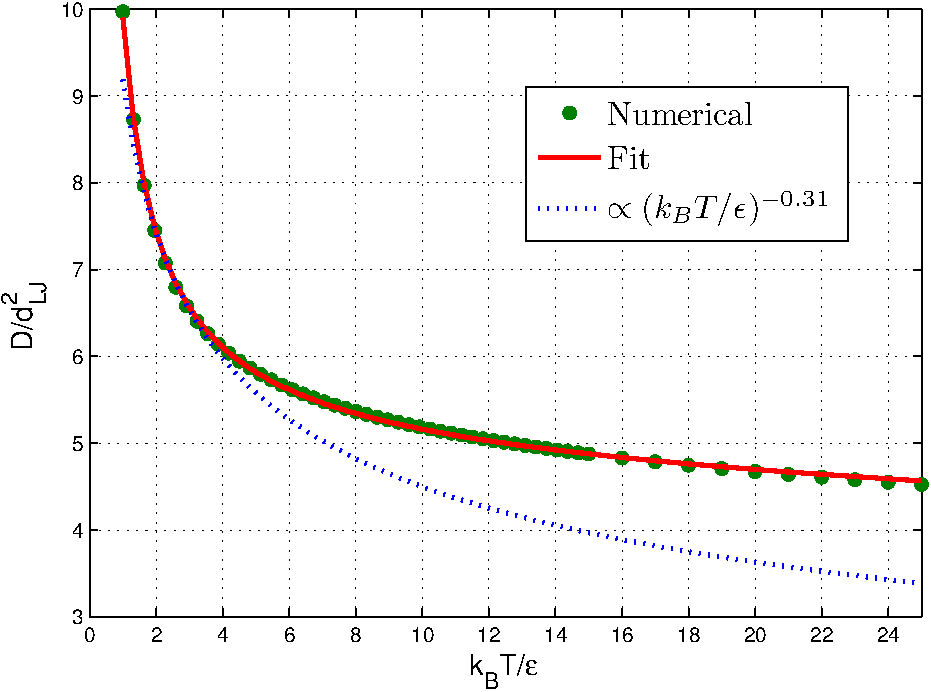
\includegraphics[scale=0.6]{Chapter4/IMG/shear_LJ3.pdf}
	\caption{
		The parameter $D$~\eqref{shear_CE_viscosity} as a function of $k_BT/\epsilon$ for the Lennard-Jones potential~\eqref{Lennard_Jones_chapter}, which is fitted by $D/d_{LJ}^2=b_1(k_BT/\epsilon)^{-0.4} +b_2(k_BT/\epsilon)^{-0.45}+b_3(k_BT/\epsilon)^{-0.5}$, where $b_1=407.4, b_2=-811.9$, and $b_3=414.4$. }
	\label{shear_LJ}
\end{figure}


For argon with the potential depth $\epsilon=119.18k_B$ in Eq.~\eqref{Lennard_Jones_chapter}, the fit in Fig.~\ref{shear_LJ} covers the temperature range from 120~K to 3000~K, while the VHS model with $\mu\propto T^{0.81}$ (dotted line) works only when 240~K$<T<$360~K. For wider temperature range, more terms with different values of $\alpha_j$ and $b_j$ may be needed. We note that, however, no matter how many terms are added (as long as $\alpha_j>-1$), the computational time of the corresponding collision operator will not increase. %The reason for this will be discussed at the end of Chapter~\ref{fourier_galerkin_spectral}. 

%In the following, if the Lennard-Jones potential is not specified, the shear viscosity of argon is proportional to $T^{0.81}$, that is, the collision kernel is given by Eq.~\eqref{kernel} or Eq.~\eqref{kernel_lei} with $\alpha=0.38$.





%\subsection{Sutherland's molecular model}
%
%For a gas whose molecules are rigid attracting spheres, i.e., the intermolecular potential is described by Eq.~\eqref{Sutherland_potential} with weak attractive fields, its shear viscosity is given by the Sutherland formula:
%\begin{equation}\label{sutherland_viscosity}
%\mu=\frac{5\sqrt{\pi{m}k_BT}}{16\sigma_{T,\infty}}\frac{T}{T+T_r},
%\end{equation} 
%where $T_r$ is a reference temperature and $\sigma_{T,\infty}$ is the total cross-section in the limiting case of infinite relative velocity $v_r$. This formula reproduces the experimental data for many real gases over a considerable range of temperature~\cite{CE,Bird1994}.
%
%
%The Sutherland formula for shear viscosity can be recovered if we use the following superposition of the modified collision kernels
%\begin{equation}\label{sutherland_kernel}
%\begin{aligned}[b]
%B=&C^{''}_{1,\gamma_1}\sin^{\gamma_1}\left(\frac{\theta}{2}\right)\cos^{-\gamma_1}\left(\frac{\theta}{2}\right)v_r\\
%+&C^{''}_{-1,\gamma_2}\sin^{\gamma_2-2}\left(\frac{\theta}{2}\right)\cos^{-\gamma_2}\left(\frac{\theta}{2}\right)v_r^{-1},
%\end{aligned}
%\end{equation}
%with the two constants ${C^{''}_{1,\gamma_1}}$ and ${C^{''}_{-1,\gamma_2}}$ satisfying
%\begin{equation}
%\begin{aligned}[b]
%8\pi{C^{''}_{1,\gamma_1}}\Gamma\left(2-\frac{\gamma_1}{2}\right)\Gamma\left(2+\frac{\gamma_1}{2}\right)=2\sigma_{T,\infty},\\
%8\pi{C^{''}_{-1,\gamma_2}}\Gamma\left(2-\frac{\gamma_2}{2}\right)\Gamma\left(1+\frac{\gamma_2}{2}\right)=2\sigma_{T,\infty}T_r\frac{4k_B}{m},\\
%\end{aligned}
%\end{equation}
%where special values of $\gamma_1$ and $\gamma_2$ (i.e., $2>\gamma_1=\gamma_2>0$) can make the FSM as fast as that for the single-term collision kernel~\eqref{kernel} or~\eqref{kernel_lei}. 



\section{Normalization}\label{Normalization_FSM}

\index{normalization}
\index{Boltzmann equation}

For practical calculations, it is convenient to introduce the following dimensionless variables:
\begin{equation}\label{normalization}
\begin{aligned}[b]
    \widetilde{f}&=\frac{v_m^3}{n_0}f, \quad
     \widetilde{\bm{x}}=\frac{\bm{x}}{L}, \quad (\widetilde{\bm{v}},\widetilde{\bm{u}},\widetilde{\bm{c}})=\frac{(\bm{v},\bm{u},\bm{c})}{v_m}, \\
\widetilde{t}&=\frac{v_m}{L}t, \quad
\widetilde{\bm{a}}=\frac{L}{v_m^2}\bm{a}, \quad
\widetilde{n}=\frac{n}{n_0}, \\
 \widetilde{T}&=\frac{T}{T_0}, \ \ \ \
\widetilde{\bm{p}}=\frac{\bm{p}}{n_0k_BT_0}, \ \ \
\widetilde{\bm{q}}=\frac{\bm{q}}{n_0k_BT_0v_m},
\end{aligned}
\end{equation}
where $n_0$ is the average number density of gas molecules, $L$ is the characteristic flow length, $v_m$ is the most probable speed at the reference temperature $T_0$. 





Under these normalization, the Boltzmann equation~\eqref{Boltzmann} with the collision kernel~\eqref{kernel_lei} takes the following form
\begin{equation}  
\label{Boltzmann_dimensionless}
\begin{aligned}
\frac{\partial \widetilde{f}}{\partial\widetilde{t}}+\widetilde{\bm{v}}\cdot\frac{\partial
\widetilde{f}}{\partial\widetilde{\bm{x}}}+\widetilde{\bm{a}}\cdot\frac{\partial
\widetilde{f}}{\partial \widetilde{\bm{v}}}=Q^+-\nu \tilde{f}.
  \end{aligned}
\end{equation}
Here, the gain term of the collision operator is  
\begin{equation}\label{coll_gain_normalization}
Q^+=\frac{1}{\text{Kn}'}\iint
\sin^{\alpha+\gamma-1}\left(\frac{\theta}{2}\right)\cos^{-\gamma}\left(\frac{\theta}{2}\right)\widetilde{v}_r^\alpha
\widetilde{f}(\widetilde{\bm{v}}'_{\ast})\widetilde{f}(\widetilde{\bm{v}}')d\Omega d\widetilde{\bm{v}}_\ast,
\end{equation}
while the loss term of the collision operator is $\nu\tilde{f}$, where the collision frequency is
\begin{equation}\label{coll_fre}
\nu=\frac{1}{\text{Kn}'}\iint
\sin^{\alpha+\gamma-1}\left(\frac{\theta}{2}\right)\cos^{-\gamma}\left(\frac{\theta}{2}\right)\widetilde{v}_r^\alpha
\widetilde{f}(\widetilde{\bm{v}}_{\ast})d\Omega d\widetilde{\bm{v}}_\ast,
\end{equation}
and 
\begin{equation}\label{Knudsen}
{\text{Kn}'}=\frac{64\sqrt{2}^\alpha}{5}\Gamma\left(\frac{\alpha+\gamma+3}{2}\right)
\Gamma\left(2-\frac{\gamma}{2}\right)\text{Kn}.
\end{equation}
It should be noted that in DSMC, the MFP of VHS model (i.e., $\lambda_{vhs}$ in Eq.~(4.52) in Ref.~\cite{Bird1994}) is frequently used. In order to compare the numerical results obtained from FSM and DSMC, the following relation should be taken into account:
\begin{equation}\label{Kn_VHS}
\begin{aligned}[b]
	%\lambda=\frac{15\pi}{2(7-2\omega)(5-2\omega)}\lambda_{VHS},	\quad\text{or}\quad 
	\text{Kn}=\frac{15\pi}{2(7-2\omega)(5-2\omega)}\text{Kn}_{vhs}.
	 \end{aligned}
\end{equation} 


\index{Lennard-Jones potential}
For the Lennard-Jones potential, when the collision kernel is approximated by Eq.~\eqref{kernel_spectral}, the term
$\sin^{\alpha+\gamma-1}(\theta/2)\cos^{-\gamma}(\theta/2){v}_r^\alpha/\text{Kn}'$
in Eqs.~\eqref{coll_gain_normalization} and~\eqref{coll_fre} should be replaced by
\begin{equation}\label{LJ_kernel}
\frac{5\sum_{j=1}^3{}b_j  (k_BT_0/2\epsilon)^{(\alpha_j-1)/2} \sin^{\alpha_j-1}({\theta}/{2})
	\widetilde{v}_r^{\alpha_j}/{\Gamma(\frac{\alpha_j+3}{2})}}
{64\sqrt{2}\text{Kn}\sum_{j=1}^3b_j(k_BT_0/\epsilon)^{(\alpha_j-1)/2}}.
\end{equation}
%A similar expression can be given for Sutherland's potential.


Considering the above normalization scheme, the normalized macroscopic quantities are related to the normalized VDF as follows:
\begin{equation}
\begin{aligned}[b]
[\widetilde{n},\widetilde{\bm{u}}, \widetilde{T}, \widetilde{p}_{ij}, \widetilde{q}_{i}]
=\int \left[1,\widetilde{\bm{v}},\frac{2}{3\widetilde{n}}\widetilde{c}^2, 2\widetilde{c}_i\widetilde{c}_j,\widetilde{c}^2\widetilde{c}_i\right]
\widetilde{f}d\widetilde{\bm{v}}.
\end{aligned}
\end{equation}
For simplicity, the tildes on normalized quantities will be omitted hereafter. 


\section{Fast spectral method}\label{single_carleman}

The numerical approximation of the Boltzmann collision operator by the FSM is introduced. For its main properties we refer to the original paper by Mouhot and Pareschi~\cite{Mouhot2006}. Detailed calculations are presented because literature gives different results for the kernel mode~\cite{Mouhot2006,Filbet2006,Hu2012}.





\subsection{Carleman representation}\label{Carleman_FSM_monatomic}
\index{Carleman representation}


We rewrite the Boltzmann collision operator using the Carleman representation. With the basic identity
\begin{equation*}
\begin{aligned}[b]
2\int_{\mathbb{R}^{3}}\delta(2\bm{y}\cdot{\bm{v}_r}+y^2)f(\bm{y})d\bm{y}=&2\int_{\mathbb{R}^{3}}\delta(|\bm{y}+\bm{v}_r|^2-v^2_r)f(\bm{y})d\bm{y}\\
=&2\int_{\mathbb{R}^{3}}\delta(y^2-v^2_r)f(\bm{y}-\bm{v}_r)d\bm{y}\\
 =&{v_r}\int_{\mathbb{S}^{2}}f(v_r\Omega-\bm{v}_r)d\Omega,
\end{aligned}
\end{equation*} 
and Eq.~\eqref{collision_velocity} for the post-collision velocities, the gain part of the collision operator~\eqref{coll_gain_normalization} is rewritten as
\begin{equation}\label{Boltzmann_gain_FSM}
\begin{aligned}[b]
 Q^+
=&\frac{1}{\text{Kn}'}\iint\Theta{v_r}
  f\left(\bm{v}_{\ast}-\frac{v_r\Omega-\bm{v}_r}{2}\right)f\left(\bm{v}+\frac{v_r\Omega-\bm{v}_r}{2}\right)d\Omega d{\bm{v}}_\ast \\
=&\frac{2}{\text{Kn}'}\iint\Theta\delta(2\bm{y}\cdot{\bm{v}_r}+y^2)
  f\left(\bm{v}_{\ast}-\frac{\bm{y}}{2}\right)f\left(\bm{v}+\frac{\bm{y}}{2}\right) d\bm{y} d{\bm{v}}_\ast \\
=&\frac{4}{\text{Kn}'}\iint\Theta\delta(\bm{y}\cdot{\bm{v}_r   }+y^2)
  f(\bm{v}_{\ast}-\bm{y})f(\bm{v}+\bm{y}) d\bm{y} d{\bm{v}}_\ast \\
=&\frac{4}{\text{Kn}'}\iint\Theta\delta(\bm{y}\cdot{}\bm{z  })
  f(\bm{v}+\bm{z})f(\bm{v}+\bm{y}) d\bm{\bm{y}} d\bm{\bm{z}},
 \end{aligned}
\end{equation}
where
$\Theta=\sin^{\alpha+\gamma-1}\left({\theta}/{2}\right)\cos^{-\gamma}\left({\theta}/{2}\right)v_r^{\alpha-1}$  if we consider the simple case where the collision kernel is given by Eq.~\eqref{kernel_lei}. Other collision kernels introduced in the above section can be handled in the same way. 


Notice that in the step-by-step calculations of Eq.~\eqref{Boltzmann_gain_FSM} we have used the transformations $\bm{y}=(v_r\Omega-\bm{v}_r)/2$ and $\bm{z}=\bm{v}_\ast-\bm{v}-\bm{y}=-\bm{v}_r-\bm{y}$; also the delta function requires that $\bm{y}$ to be perpendicular to $\bm{z}$. Therefore, the deflection angle $\theta$ satisfies 
\begin{equation}
    \cos\theta=\frac{\Omega\cdot{\bm{v}_r}}{v_r}
    =\frac{-(\bm{y}-\bm{z})\cdot(\bm{y}+\bm{z})}{|\bm{y}+\bm{z}|^2}
    \overset{\bm{y}\bot{\bm{z}}}
    {=}\frac{z^2-y^2}{y^2+z^2},
\end{equation}
which results in
\begin{equation}\label{sincos}
\begin{aligned}
\sin\left(\frac{\theta}{2}\right)=\frac{|\bm{y}|}{\sqrt{y^2+z^2}},\ \ \ \ 
\cos\left(\frac{\theta}{2}\right)=\frac{|\bm{z}|}{\sqrt{y^2+z^2}}.
\end{aligned}
\end{equation}
Hence
$\Theta=|\bm{y}|^{\alpha+\gamma-1}|\bm{z}|^{-\gamma}$ and the collision
operator is simplified to
\begin{equation}\label{ccc}
\begin{aligned}[b]
 Q=\frac{4}{\text{Kn}'}\iint&d\bm{y} d\bm{z}\delta(\bm{y}\cdot{}\bm{z})|\bm{y}|^{\alpha+\gamma-1}|\bm{z}|^{-\gamma}\\
 &\times [f(\bm{v}+\bm{z})f(\bm{v}+\bm{y})-f(\bm{v}+\bm{y}+\bm{z})f(\bm{v})].
 \end{aligned}
\end{equation}


\subsection{Fourier-Galerkin spectral method}\label{fourier_galerkin_spectral}

In FSM, the VDF is periodized on the domain $\mathcal{D}_L=[-L_v,L_v]^3$. We adopt uniform grid points in the velocity space:
\begin{equation}
v_k(j_k)=2\frac{L_v}{N_k}j_k, \quad (k=1,2,3)
\end{equation}
where $j_k\in[-N_k/2, -N_k/2+1,\cdots, N_k/2-1]$ and $N_k$ is the number of velocity grid points in the $k$-th velocity direction. Suppose $\mathcal{B}_S$, a sphere of radius $S$ centered at the origin, is the support of VDF. Usually the minimum value 
$L_v=(3+\sqrt2)S/2$ is chosen to avoid the aliasing error caused by the periodicity of VDF~\cite{Pareschi2000}. The VDF is then approximated by a truncated Fourier series,
\begin{eqnarray}
    f(\bm{v})&=&\sum_{\bm{j}=-(N_1,N_2,N_3)/2}^{(N_1,N_2,N_3)/2-1}
    \hat{f}_{\bm{j}}\exp(i\xi_{\bm{j}}\cdot{}\bm{v}), \label{fourier}\\
    \hat{f_{\bm{j}}}&=&\frac{1}{(2L_v)^3}
    \int{}f(\bm{v})\exp(-i\xi_{\bm{j}}\cdot{}\bm{v})d\bm{v},
    \label{inverse_FSM_fourier}
\end{eqnarray}
where $\xi_{\bm{j}}=\bm{j}\pi/L$ are the frequency components with $\bm{j}=(j_1,j_2,j_3)$. 


The Boltzmann collision operator~\eqref{ccc} is also truncated, with the infinite velocity space replaced by the finite one in ${\mathcal{B}_R}$, where the truncation radius $R$ satisfies~\cite{Mouhot2006,Filbet2006}:
\begin{equation}\label{velocity_truncation}
R\ge\sqrt{2}S.
\end{equation} 
Numerical analysis in Fig.~\ref{test_R} will show that, however, $R$ cannot be larger than $L$. Expanding the truncated collision operator by Fourier series, we find that the $\bm{j}$-th spectrum of the truncated collision operator is related to spectrum $\hat{f}$ as:
\begin{equation}\label{mo_monatomic_de}
   \widehat{Q}_{\bm{j}}= \sum_{\bm{l}+\bm{m}=\bm{j} \atop
    \bm{l},\bm{m}=-(N_1,N_2,N_3)/2}^{{(N_1,N_2,N_3)}/2-1}\hat{f}_{\bm{l}}\hat{f}_{\bm{m}}[\beta(\bm{l},\bm{m})-\beta(\bm{m},\bm{m})],
\end{equation}
where $\bm{l}=(l_1,l_2,l_3)$, $\bm{m}=(m_1,m_2,m_3)$, and the kernel mode
$\beta(\bm{l},\bm{m})$ is simplified to 
\begin{equation}\label{kernel_FSM_mode0}
\begin{aligned}[b]
\beta(\bm{l},\bm{m})=&\frac{4}{\text{Kn}'}\iint
\delta(\bm{y}\cdot{\bm{z}})|\bm{y}|^{\alpha+\gamma-1}|\bm{z}|^{-\gamma}
\exp(i\xi_{\bm{l}}\cdot{\bm{y}}+i\xi_{\bm{m}}\cdot{\bm{z}})d\bm{y}d\bm{z}\\
   =&\frac{1}{\text{Kn}'}\int\int \delta(\bm{e}\cdot{\bm{e}'})
              \left[\int_{-R}^R|\rho|^{\alpha+\gamma}\exp(i\rho\xi_{\bm{l}}\cdot{\bm{e}})d\rho\right]\\
              &\ \ \ \ \ \ \ \ \ \ \ \ \ \ \ \ \ \ \ \ \times\left[\int_{-R}^R|\rho'|^{1-\gamma}\exp(i\rho'\xi_{\bm{m}}\cdot{\bm{e}'})d\rho'\right]d\bm{e}'d\bm{e} \\
=&\frac{1}{\text{Kn}'}\int_{\mathbb{S}^2}
    \phi_{\alpha+\gamma}(\xi_{\bm{l}}\cdot{\bm{e}})
    \left[\int_{\mathbb{S}^2}\delta(\bm{e}\cdot{\bm{e}'})\phi_{1-\gamma}(\xi_{\bm{m}}\cdot{}\bm{e}')d\bm{e}'\right]d\bm{e},
\end{aligned}
\end{equation}
with $\bm{e}, \bm{e}'$ being the unit vectors in the sphere $\mathbb{S}^{2}$, and
\begin{equation}\label{phi_FSM_expression}
    \phi_\delta(s)=2\int_{0}^R\rho^\delta\cos\left(\rho{s}\right)d\rho.
\end{equation}


\begin{figure}[t]
	\centering
	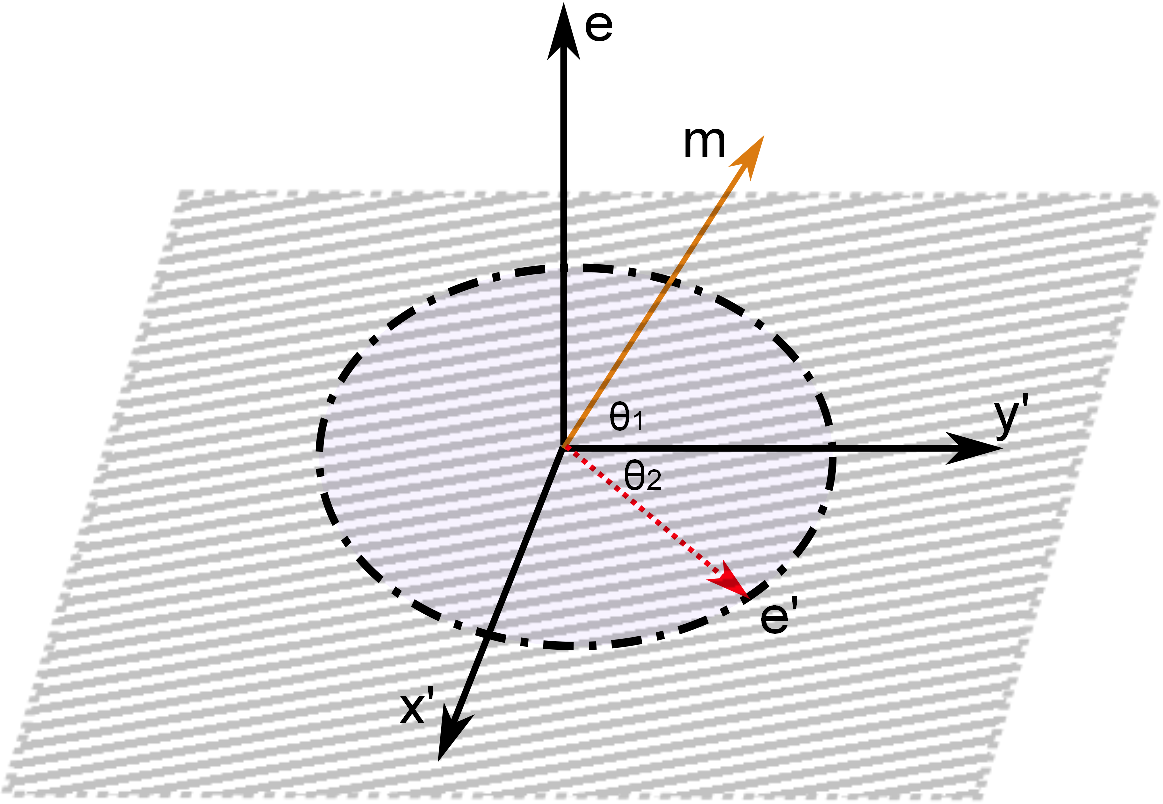
\includegraphics[width=7.5cm]{Chapter4/IMG/demo.pdf}
	\caption{
		Demonstration of the integral with respect to $\bm{e}'$ used in the calculation of kernel mode~\eqref{kernel_FSM_mode0}. When the vector $\bm{e}$ is fixed, we can make the $x'y'$ plane perpendicular to $\bm{e}$ and $m$ fall in the $ey'$ plane. The vector $\bm{e}'$ degenerates to a two-dimensional vector characterized by the polar angle $\theta_2$ varying from 0 to $2\pi$. The polar and azimuthal angles of $\bm{e}'$ in the new coordinate system are $\theta$ and $\pi/2-\theta_2$, respectively, and the angle between the vector $\bm{m}$ and $y'$-axis is $\theta_1$. 
	} 
	\label{demo}
\end{figure}


Equation~\eqref{kernel_FSM_mode0} can be simplified further. We construct a new Cartesian coordinate system, where its ${z}'$ axis is parallel to $\bm{e}$, the $y'$ axis is just the projection of vector $\bm{m}$ into the plane $e_\bot$ perpendicular to the $z'$ axis, and the $x'$ axis is in the plane $e_\bot$ and perpendicular to the $y'$ axis, see Fig.~\ref{demo}. Suppose the polar and azimuthal angles of $\bm{e}'$ in the new coordinate system are $\theta$ and $\pi/2-\theta_2$, respectively, and the angle between the vector $\bm{m}$ and $y'$-axis is $\theta_1$. Then, we have $\delta(\bm{e}\cdot{\bm{e}'})=\delta(\cos\theta)$ so that $\int_0^\pi g(\theta)\delta(\cos\theta)d\theta=g(\pi/2)$ for smooth function $g(\theta)$, $\xi_{\bm{m}}\cdot{}\bm{e}'=|\xi_{\bm{m}}|\cos\theta_1\cos\theta_2$, and the kernel mode becomes
\begin{equation}\label{kernel_mode2}
\begin{aligned}[b]
\beta(\textbf{l},\textbf{m})&=\frac{1}{\text{Kn}'}\int_{\mathcal{S}^2}d\textbf{e} \phi_{\alpha+\gamma}(\xi_\textbf{l}\cdot{\textbf{e}}) \\
&\times
\left[\int_0^{2\pi}\int_0^\pi\delta(\cos\theta)\phi_{1-\gamma}(|\xi_\textbf{m}|
\cos\theta_{1}\cos\theta_2)d\theta{d\theta_2}\right]\\
&=\frac{1}{\text{Kn}'}\int_{\mathcal{S}^2}\phi_{\alpha+\gamma}(\xi_\textbf{l}\cdot{\textbf{e}})
\left[\int_0^{2\pi} \phi_{1-\gamma}(|\xi_\textbf{m}|\cos\theta_1\cos\theta_2)d\theta_2\right]d\textbf{e}\\
&=\frac{2}{\text{Kn}'}\int_{\mathcal{S}^2}\phi_{\alpha+\gamma}(\xi_\textbf{l}\cdot{\textbf{e}})
\cdot\psi_{\gamma}(|\xi_\textbf{m}|\cos\theta_1)d\textbf{e},
\end{aligned}
\end{equation}
%\begin{equation}\label{kernel_mode2}
%\begin{aligned}[b]
%\beta(\bm{l},\bm{m})
%        &=\frac{1}{\text{Kn}'}\int_{\mathcal{S}^2}\phi_{\alpha+\gamma}(\xi_{\bm{l}}\cdot{\bm{e}})
%\left[\int_0^{2\pi} \phi_{1-\gamma}(|\xi_{\bm{m}}|\cos\theta_1\cos\theta_2)d\theta_2\right]d\bm{e}\\
%        &=\frac{2}{\text{Kn}'}\int_{\mathcal{S}^2}\phi_{\alpha+\gamma}(\xi_{\bm{l}}\cdot{\bm{e}})
%                \cdot\psi_{\gamma}(|\xi_{\bm{m}}|\cos\theta_1)d\bm{e},
%\end{aligned}
%\end{equation}
where
\begin{equation}\label{psi_FSM_expression}
 \psi_{\gamma}(s)=\int_0^\pi\phi_{1-\gamma}(s\cos\theta_2)d\theta_2=2\pi\int_0^R \rho^{1-\gamma} J_0(\rho s)d\rho, %=2\pi{R}\frac{J_1(Rs)}{s},
\end{equation}
with $J_0$ being the zeroth-order Bessel function.


Note that $\xi_{\bm{l}}$ and $\xi_{\bm{m}}$ in Eq.~\eqref{kernel_mode2} appear in two functions. If they also appear in two different functions in the final form of $\beta(\bm{l},\bm{m})$, Eq.~\eqref{mo_monatomic_de} can be calculated effectively by the FFT-based convolution. The separation of $\bm{l}$ and $\bm{m}$ in Eq.~\eqref{kernel_mode2} can be realized approximately using the numerical quadrature. Two different methods will be employed and compared:
\begin{itemize}
    \item  in the first method, $\beta(\bm{l},\bm{m})$ is calculated numerically in spherical coordinates by the trapezoidal rule. Suppose the polar and azimuthal angles of the unit vector $\bm{e}$ are $\theta$ and $\varphi$, respectively. We divide each region $0\le\theta\le\pi$ and $0\le\varphi\le\pi$ (for symmetry) into $M$ sections: $\theta_p=p\pi/M$ and $\varphi_q=q\pi/M$ with $p,q=1,2,\cdots,M$. Then the kernel mode~\eqref{kernel_mode2} is approximated by
    \begin{equation}\label{kernel_FSM_mode}
    \begin{aligned}[b]
    \beta(\bm{l},\bm{m})\simeq\frac{4\pi^2}{\text{Kn}'M^2}\sum_{p,q=1}^{M-1,M}
    \phi_{\alpha+\gamma}(\xi_{\bm{l}}\cdot{\bm{e}_{\theta_p,\varphi_q}})
        \psi_{\gamma}(\xi^\perp_{\bm{l}})
        \cdot\sin\theta_p,
        \end{aligned}
    \end{equation}
    where 
    \begin{equation}
    \xi^\perp_{\bm{l}}=\sqrt{|\xi_{\bm{m}}|^2-(\xi_{\bm{m}}\cdot{\bm{e}}_{\theta_p,\varphi_q})^2}.
    \end{equation}
           
    \item  in the second method, $\beta(\bm{l},\bm{m})$ is approximated by a  Gauss-Legendre quadrature of order $M$ (see the Matlab code in Appendix~\ref{appen_GaussLegendre}):
    \begin{equation} \label{kernel_FSM_modee}
    \begin{aligned}[b]
    \beta(\bm{l},\bm{m})\simeq\frac{4}{\text{Kn}'}\sum_{p,q=1}^{M}{\omega_p\omega_q}
    \phi_{\alpha+\gamma}(\xi_{\bm{l}}\cdot{\bm{e}_{\theta_p,\varphi_q}})\psi_{\gamma}(\xi^\perp_{\bm{l}})\cdot\sin\theta_p,
        \end{aligned}
    \end{equation}
            where $\theta_p\ (\varphi_q)$ and $\omega_p\  (\omega_q)$ are the $p\ (q)$-th point and weight in the Gauss-Legendre quadrature with  $\theta, \varphi\in[0,\pi]$, and the unit vector is expressed as
            \begin{equation}
           \bm{e}_{\theta_p,\varphi_q}=(\sin\theta_p\cos\varphi_q,\sin\theta_p\sin\varphi_q,\cos\theta_p).
            \end{equation}
\end{itemize}

\begin{figure}[t]
	\centering
	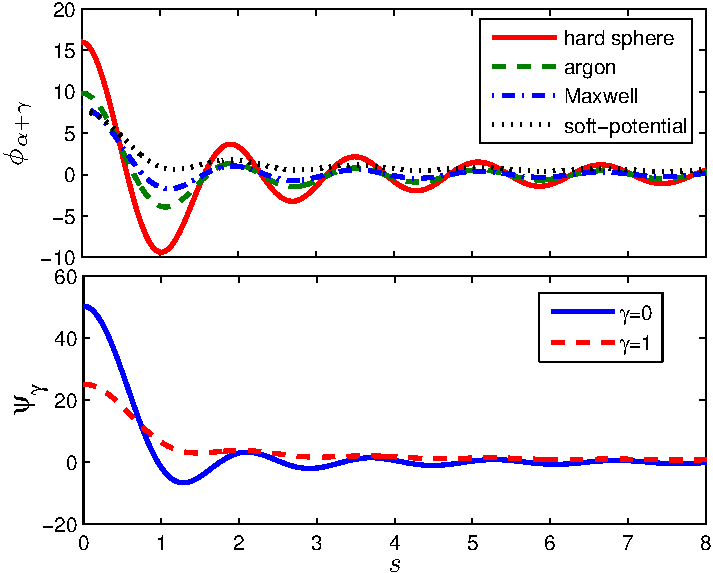
\includegraphics[width=10cm]{Chapter4/IMG/phi_psi2.pdf}
	\caption{
		Profiles of $\phi_{\alpha+\gamma}$  and $\psi_\gamma$ according to Eqs.~\eqref{phi_FSM_expression} and~\eqref{psi_FSM_expression} when $R=4$ and $\gamma=0$. Because of symmetry, the region $s<0$ is not plotted. For the soft potential, we use $\alpha=-0.4$ and the shear viscosity is proportional to $T^{1.2}$.
	}
	\label{phi_psi}
\end{figure}

The analytical form of $\phi_{\alpha+\gamma}(s)$ can be obtained when $\alpha+\gamma$ is an integer. For instance, when $\gamma=0$, for Maxwell molecules $(\alpha=0)$ and HS $(\alpha=1)$ molecules, we have
\begin{equation}\label{int_res}
  \begin{aligned}[b]
    \phi_0(s)=\frac{2\sin(Rs)}{s},\\
    \phi_1(s)=\frac{2R\sin(Rs)}{s}-\frac{4\sin^2(Rs/2)}{s^2},
  \end{aligned}
\end{equation}
while for  other cases $\phi_{\alpha+\gamma}(s)$ and $\psi_{\gamma}(s)$ can be accurately calculated by Gauss-Legendre quadrature numerically. Fig.~\ref{phi_psi} shows typical decaying-oscillating profiles of the two functions $\phi_{\alpha+\gamma}$ and $\psi_\gamma$, where  the quasi-period of oscillation is about $2\pi/R$.




Note that in the VHS model, $-3<\alpha\le1$. From Eq.~\eqref{phi_FSM_expression} it follows that $\delta$ is restricted to the region $(-1,+\infty)$. Therefore, $\alpha+\gamma>-1$ and $1-\gamma>-1$. In the original collision kernel proposed by Mouhot and Pareschi~\cite{Mouhot2006}, $\gamma=0$, so that $\alpha$ is restricted in the region $(-1,1]$. This means that the original collision kernel cannot deal with general forms of soft potentials. In our modified collision kernel~\eqref{kernel_lei}, if we let $\gamma\rightarrow2$, $\alpha$ can cover the whole region $(-3,1]$, thus extending the applicability of FSM to all inverse power-law potentials except the Coulomb potential. 


It should also be noted that for the Lennard-Jones potential, the storage of the kernel modes and computational cost of the collision operator is exactly the same as that for the single-term collision kernel~\eqref{kernel} or~\eqref{kernel_lei}. 
%For the collision kernel~\eqref{sutherland_kernel} of the Sutherland potential, if we let $\gamma_1=\gamma_2$, the storage and computational cost will also be the same as the single-term collision kernel. 
For the existence of $\phi_{1+\gamma_1}$, $\psi_{1-\gamma_1}$, $\phi_{-1+\gamma_2}$, and $\psi_{1-\gamma_2}$, one should choose $-2<\gamma_1<2$ and $0<\gamma_2<2$. Therefore, we choose $0<\gamma_1=\gamma_2<2$. If $\gamma_1\neq\gamma_2$, the storage and computational cost will be twice of that of the single-term collision kernel~\eqref{kernel_lei}.


\subsection{Detailed implementation}

The detailed procedure to calculate the Boltzmann collision operator is now outlined. Let us assume Eq.~\eqref{kernel_mode2} is approximated by the trapezoidal rule. First, the kernel modes is pre-computed and stored. The storage of $\phi_{\alpha+\gamma}(\xi_{\bm{l}},\theta_p,\varphi_q)$ and $\psi_{\gamma}(\xi_{\bm{m}},\theta_p,\varphi_q)$ requires $2M(M-1)N_1N_2N_3$ units of compute memory. We also need $N_1N_2N_3$ units of storage for
\begin{equation}\label{phi_loss}
\phi_{loss}=\sum_{p,q=1}^{M-1,M}\phi_{\alpha+\gamma}(\xi_{\bm{m}},\theta_p,\varphi_q)
    \psi_{\gamma}(\xi_{\bm{m}},\theta_p,\varphi_q)\sin\theta_p,
\end{equation}
which is used to calculate the collision frequency in Eq.~\eqref{coll_fre}. For space-homogeneous problems, such storage is relatively large when compared to the storage of VDF. However, when it comes to space-inhomogeneous problems, the storage will be relatively small because different spatial grids share the same kernel modes. 


\begin{figure}[t]
	\centering
	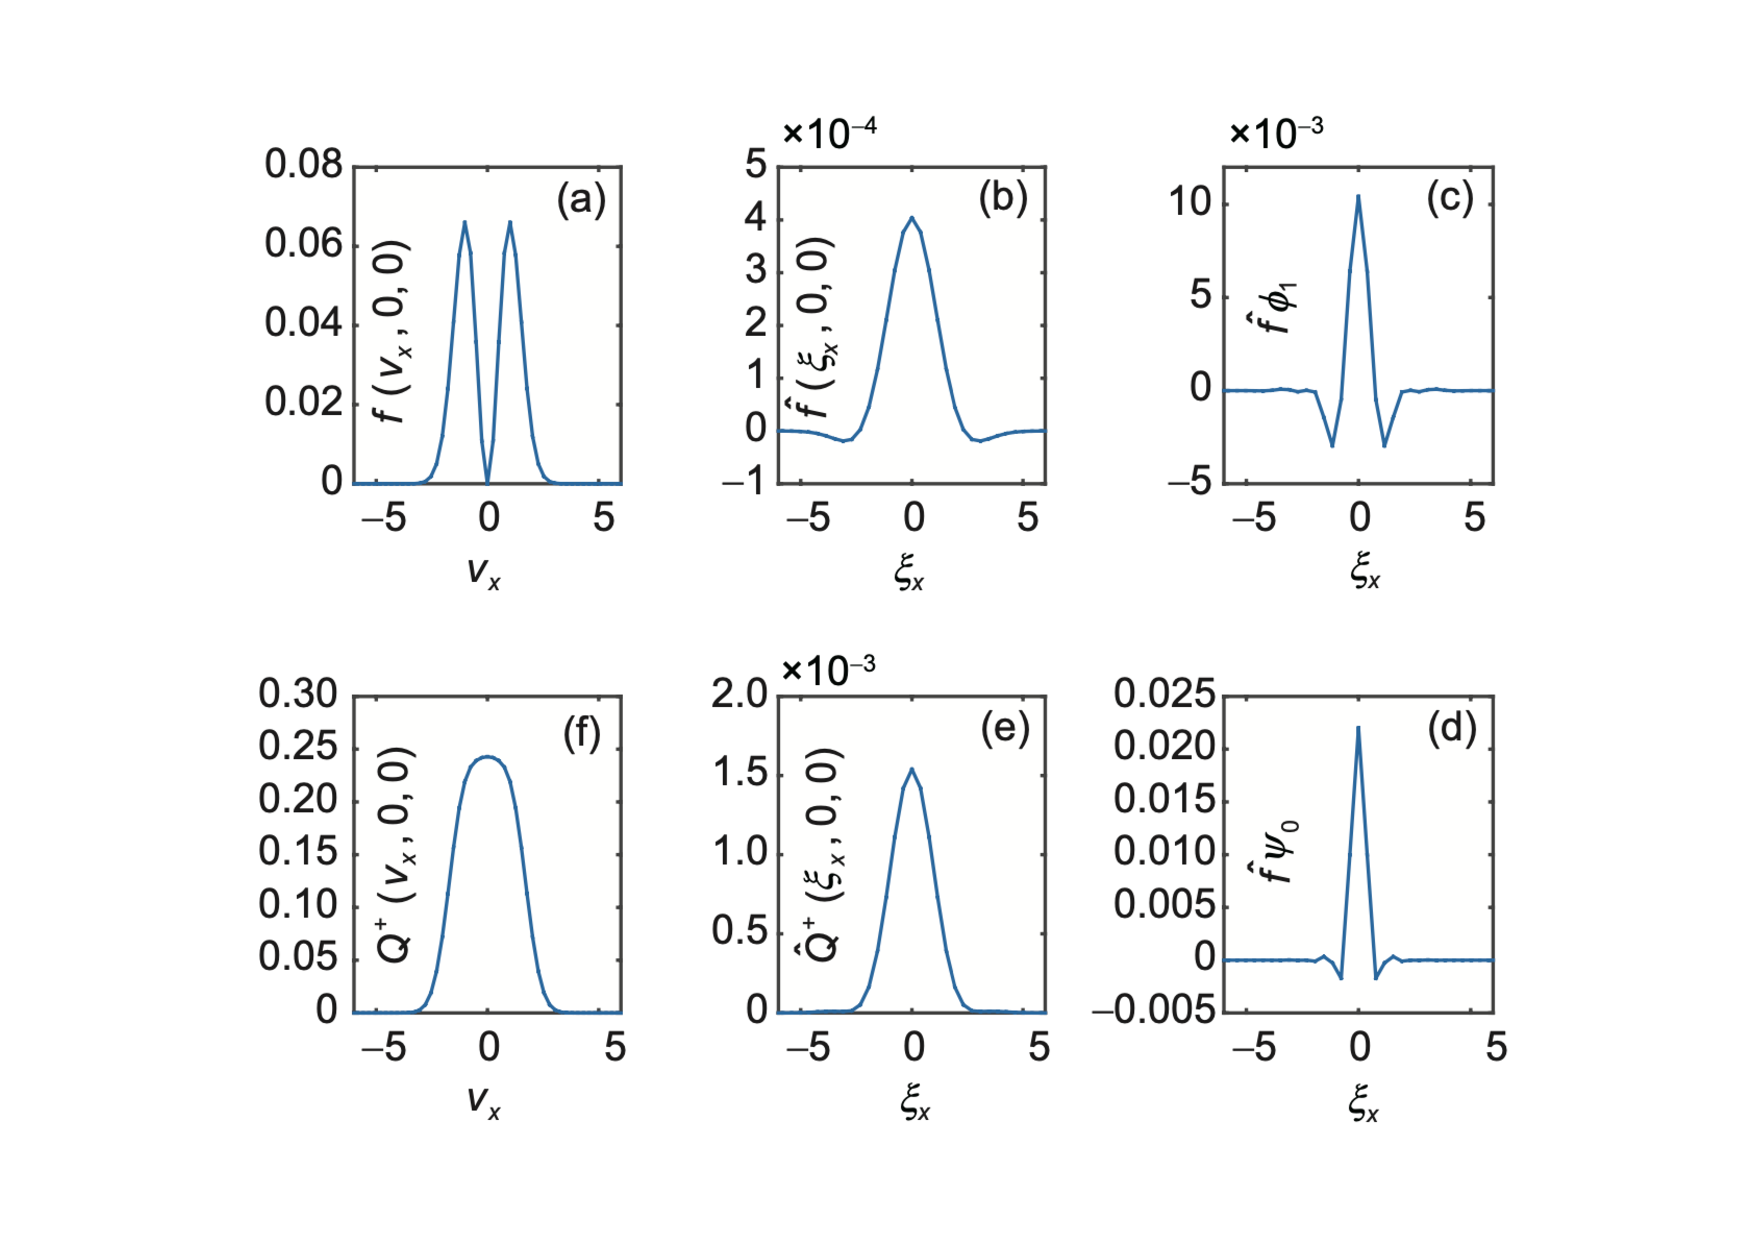
\includegraphics[scale=0.5]{Chapter4/IMG/FSM_demo.pdf}
	\caption{
		Numerical implementation of the FSM for the gain part of Boltzmann collision operator~\eqref{coll_gain_normalization}. Given the VDF in (a), its spectrum in obtained in (b) by inverse FFT. Then the spectrum is respectively multiplied with the kernel modes $\phi$ and $\psi$ (the results are in (c) and (d), respectively), and their convolution is shown in (e). The FFT of (e) gives the gain part of the Boltzmann collision operator for specific combination of $p$ and $q$ in (f). Summering $Q^+$ for all combinations of $p$ and $q$ gives the gain part of the Boltzmann collision operator. Note that the whole process is done in three-dimensional velocity space and spectrum space, but for clarity only the one-dimensional results are shown.
	  }
	\label{FSM_demo}
\end{figure}


Second, we obtain the spectrum of VDF by applying the inverse FFT to $f$. Then, with Eq.~\eqref{kernel_FSM_mode}, Eq.~\eqref{mo_monatomic_de} becomes 
\begin{equation*}
\begin{aligned}[b]
  \widehat{Q}_{\bm{j}}\approx &\underbrace{\frac{4\pi^2}{\text{Kn}'M^2}\sum_{p,q=1}^{M-1,M} \sum_{\bm{l}+\bm{m}=\bm{j} }[\hat{f}_{\bm{l}}{\phi_{\alpha+\gamma}(\xi_{\bm{l}},\theta_p,\varphi_q)}]\cdot[\hat{f}_{\bm{m}}{\psi_{\gamma}(\xi_{\bm{m}},\theta_p,\varphi_q)}]}_{gain}\cdot\sin\theta_p
  \\
  &\underbrace{-\frac{4\pi^2}{\text{Kn}'M^2}\sum_{\bm{l}+\bm{m}=\bm{j} }\hat{f}_{\bm{l}}\cdot[\hat{f}_{\bm{m}}{\phi_{loss}}]}_{loss}.
\end{aligned}
\end{equation*}

The loss term can be effectively calculated by FFT-based convolution, using the zero-padding technique~\cite{Canuto1998}. For the gain term, one has to do FFT-based convolution for each pair of $(p,q)$, that is, $M(M-1)$ times. The implementation is listed in Steps 2, 3, and 4 in the algorithm 1 of Appendix~\ref{appen_FSM}. Finally, the collision operator $Q$ is calculated by applying the FFT to $\widehat{Q}$ (Step 5). The whole process is visualized in Fig.~\ref{FSM_demo}.

Note that in algorithm 1 the zero-padding technique is employed to eliminate the aliasing error in FFT-based convolution. This process is accurate for arbitrary values of $t_1$ and $t_2$ (defined in Appendix~\ref{appen_FSM}) when the padding size in each direction is larger than one half of the velocity grid number. Considering the fact that the spectrum $\hat{f}$ is non-zero only in the central region of frequency domain, we can expedite the calculation by ignoring zero-padding. This leads to the simpler and faster algorithm 2: numerical simulations show that both algorithms produce identical results, but the algorithm 2 is about 4 times faster than the algorithm 1.


Now we see that the computational cost of FSM is $O(M^2N^3\log{}N)$, where $N$ is the same order as $N_1,N_2$ and $N_3$. Note that $\bm{l}$ and $\bm{m}$ are not separable in classical spectral methods, and the computational cost of Eq.~\eqref{mo_monatomic_de} is $O(N^6)$~\cite{Gamba2009,Pareschi2000}. A rough estimate of the speed-up can be given. In algorithm 2, one needs to do $2M(M-1)+2$ times FFT (the array size is $N_1\times{N_2}\times{N_3}$), while in classical spectral methods the computational cost is the same with one direct convolution of one complex and one real array of size $N_1\times{N_2}\times{N_3}$. For comparison, we take $M=7$ and run our Matlab (version 2012a) programs on a PC with an Intel Xeon 3.3 GHz CPU. For $N=32$ (or 64), algorithm 2 is about 18 (or 62) times faster than the classical spectral methods. Further speed-up can be achieved by reducing the value of $M$, say, to 5. 

%As will shown in Chapter~\ref{chap:linearized}, for the flows with large Knudsen number there are discontinuities in the VDF; to capture the discontinuities, one needs large number of velocity grids. In this case, the FSM could be faster than the classical spectral methods by two orders of magnitude. 


\subsubsection{Conservation enforcement}%\label{conservation_single}

One of the drawbacks of FSM, as with any spectral methods in the approximation of Boltzmann collision operator, is that it does not exactly conserve the momentum and energy. To ensure the conservation of momentum and energy, the method of Lagrangian multipliers can be employed~\cite{Gamba2009}: after the collision operator $Q$ is approximated, we construct $Q^{new}$ by minimizing the function $\sum_{\bm{j}}(Q_{\bm{j}}-Q_{\bm{j}}^{new})^2$ under the constraints $\sum_{\bm{j}} Q_{\bm{j}}^{new}=\sum_{\bm{j}} \bm{v}Q_{\bm{j}}^{new}=\sum_j {v^2}Q_{\bm{j}}^{new}=0$, yielding
\begin{equation*}\label{Lagrangian1}
{Q}^{new}={Q}-(\lambda_n+\lambda_{\bm{v}}\cdot{}\bm{v}+\lambda_e {v^2}),
\end{equation*}
where the five Lagrangian multipliers satisfy
\begin{equation*}
\begin{aligned}[b]
\sum_{\bm{j}} Q=\sum_j (\lambda_n+\lambda_{\bm{v}}\cdot{}\bm{v}+\lambda_e |\bm{\bm{v}}|^2), \\
\sum_{\bm{j}} \bm{v}Q=\sum_j \bm{v}(\lambda_n+\lambda_{\bm{v}}\cdot{}\bm{v}+\lambda_e {v^2}), \\
\sum_{\bm{j}} {v^2} Q=\sum_j {v^2}(\lambda_n+\lambda_{\bm{v}}\cdot{}\bm{v}+\lambda_e {v^2}).
\end{aligned}
\end{equation*}

Since the errors for the momentum and energy in FSM are spectrally small~\cite{Mouhot2006}, the Lagrangian multipliers are very small. In practice, we normally do not use  conservation enforcement if the steady-state solution of the Boltzmann equation can be quickly found.



\subsection{Non-uniform discretization of velocity space}

In the simulation of rarefied gas flows with large Knudsen numbers, the ``over concentration'' phenomenon are frequently encountered~\cite{Takata2011}, where the VDF concentrates or has sharp variations around $v\sim0$ due to the wall effect. To tackle this problem, the molecular velocity space should be discretized non-uniformly, with more points placed near $v=0$. In microflows, we usually use the following non-uniform discretization:
\begin{equation}\label{nonuniform_v}
v_i=\frac{L_v}{(N_v-1)^\imath}(-N_v+1,-N_v+3,\cdots,{N_v-1})^\imath,
\end{equation}
where $\imath$ is a positive odd number, $L_v$ is the velocity bound, and $N_v$ is the total number of discretized velocity in the $i$-th direction. 


However, the frequency space must be discretized uniformly, otherwise the FFT-based convolution cannot be applied efficiently. This means that Steps 2 and 3 in the algorithm of Appendix~\ref{appen_FSM} remain unchanged, but the Fourier transform in Steps 1 and 4 is calculated by direct summation. Fortunately, the computational cost can be reduced by considering the following two factors:
\begin{itemize}
	\item the number of discretized frequency components $N_\xi$ can be different from the corresponding velocity components $N_v$. In fact, $N_\xi$ can be much smaller than $N_v$ due to the spectral accuracy of FSM; hence the computational cost of the convolution is $O(M^2N_{\xi}\ln{N_{\xi}})$.
	
	\item in the rectangular Cartesian coordinates, the Fourier transform in Steps 1 and 4 can be done by direct summation in each direction sequentially, thus the cost will be at the order of $N_v^3N_\xi\ln{}N_v$. This cost is certainly higher than the FFT on uniform grids, but is only comparable to the FFT-based convolution in Steps 2 and 3. 
\end{itemize}
Therefore, compared to the uniform discretization with large number of velocity grids, the use of non-uniform velocity grids will not only reduce computational memory, but also computational time.

%The number of frequency components in the $\xi_1$ and $\xi_3$ directions are $N_1'N_3'=24\times24$, and there are $N_2'$ frequency components in the $\xi_2$ direction. The FFT is used in the $v_1$ and $v_3$ directions, while in the $v_2$ direction the direct sum is implemented: for nonuniform velocity grids~\eqref{nonuniform_v}, we use $\sum_m{}g(v_{2m})w_m$ to approximate  $\int{}g(v_2)dv_2$, where 

%\begin{equation}
%w_m=\imath{}L(-N_2+1,-N_2+3,\cdots,{N_2-1})^{\imath-1}/(N_2-1)^\imath.
%\end{equation}
%The resulting  overall computational cost is $O(N_2N_2'N_1'N_3'\ln(N_1'N_3'))$, which is comparable to the FFT-based convolution sum of equation~\eqref{detailed_linear_half}. 
%
%
%The calculation of $\mathcal{L}_g(h^k)$ is as follows: when $h^k$ is known, we obtain $\hat{\mathcal{L}}_g$ from equation~\eqref{detailed_linear_half}. Then we obtain $\mathcal{L}_g(h^k)$ by applying the inverse FFT to $\hat{\mathcal{L}}_g$:
%$
%\mathcal{L}_g(h^k)=\sum_{\textbf{j}=-\textbf{N}/2}^{\textbf{N}/2-1}\hat{\mathcal{L}}_g(j)\exp(i\xi_\textbf{j}\cdot{}\textbf{v})
%$. 





\section{Accuracy in homogeneous relaxation}
\index{homogeneous relaxation}

To assess the accuracy of FSM, the relax-to-equilibrium process of Maxwell molecules ($\alpha,\gamma=0$) is considered. This is a spatial-homogeneous problem, where the Boltzmann equation becomes 
\begin{eqnarray}
 \frac{\partial {f}}{\partial{t}}=\frac{1}{\text{Kn}'}\iint
\sin^{-1}\left(\frac{\theta}{2}\right)
[{f}({\bm{v}}'_{\ast}){f}({\bm{v}}')-{f}({\bm{v}}_\ast)
  {f}({\bm{v}})]d\Omega d{\bm{v}}_\ast. 
  \label{Boltzmann_homogeneous}
\end{eqnarray}
Without loss of generality, we choose $\text{Kn}'=32\pi/5$. And for simplicity we consider the uniform discretization of molecular velocity space.

\subsection{Bobylev-Krook-Wu solution}
\index{Bobylev-Krook-Wu}

Equation~\eqref{Boltzmann_homogeneous} possesses the exact Bobylev-Krook-Wu (BKW) solution~\cite{BKW}:
\begin{equation}\label{initial_2}
    f(\bm{v},t)=\frac{1}{2(2\pi{K})^{3/2}}\exp\left(-\frac{{v^2}}{2K}\right)\left(\frac{5K-3}{K}+\frac{1-K}{K^2}{v^2}\right),
\end{equation}
where  $K=1-0.4\exp\left(-{t}/{6}\right)$. The evolution of the fourth- and sixth-order moments is given by
\begin{equation}\label{initial_22}
\begin{aligned}[b]
	M_4=\int fv_1^4d\bm{v}=6K-3K^2,\\ 
	M_6=\int fv_1^6d\bm{v}=45K^2-30K^3.
\end{aligned}
\end{equation}


\begin{table}[t]
	\centering
	\caption[Relative error in the approximation of the Boltzmann collision operator.]{Relative error $\sum_{\bm{j}}|Q_{\bm{j}}^{nu}-Q_{\bm{j}}^{an}|/\sum_{\bm{j}}|Q_{\bm{j}}^{an}|$ in the approximation of the Boltzmann collision operator. T (G) stands for the trapezoidal (Gauss-Legendre) quadrature used in the approximation of Eq.~\eqref{kernel_mode2}. Parameters are $L=8$ and $R=6$. } \label{table_coll} 
		\begin{tabular}{ccccccccccccccc}
			\hline
			N  &    & $M=5$    & 6       & 7        & 8         & 12       & 16       \\
			$16$& T  & 4.58E-1  & 4.73E-1 & 4.55E-1  & 4.52E-1   & 4.78E-1   & 4.83E-1  \\
			& G  & 2.10E-1  & 3.35E-1 & 2.48E-1  & 2.77E-1   & 2.74E-1   & 2.69E-1  \\
			24 & T  & 7.94E-2  & 5.20E-2 & 4.73E-2  & 3.93E-2   & 2.92E-2   & 2.59E-2  \\
			& G  & 4.61E-2  & 2.09E-2 & 9.16E-3  & 2.10E-2   & 1.72E-2   & 1.37E-2  \\
			32 & T  & 5.54E-2  & 3.51E-2 & 2.57E-2  & 1.93E-2   & 8.39E-3   & 4.75E-3  \\
			& G  & 4.26E-2  & 6.18E-3 & 6.49E-4  & 2.11E-4   & 1.86E-4   & 1.57E-4  \\
			48 & T  & 4.26E-2  & 3.88E-2 & 2.77E-2  & 2.08E-2   & 8.99E-3   & 5.01E-3  \\
			& G  & 4.31E-2  & 6.17E-3 & 6.09E-4  & 4.56E-5   & 4.94E-6   & 3.85E-6  \\
			64 & T  & 5.90E-2  & 3.87E-2 & 2.77E-2  & 2.08E-2   & 8.99E-3   & 5.02E-3  \\
			& G  & 4.30E-2  & 6.16E-3 & 6.10E-4  & 4.70E-5   & 3.87E-6   & 4.31E-6  \\
			\hline
		\end{tabular}
	\end{table}


\begin{figure}[t]
	\centering
	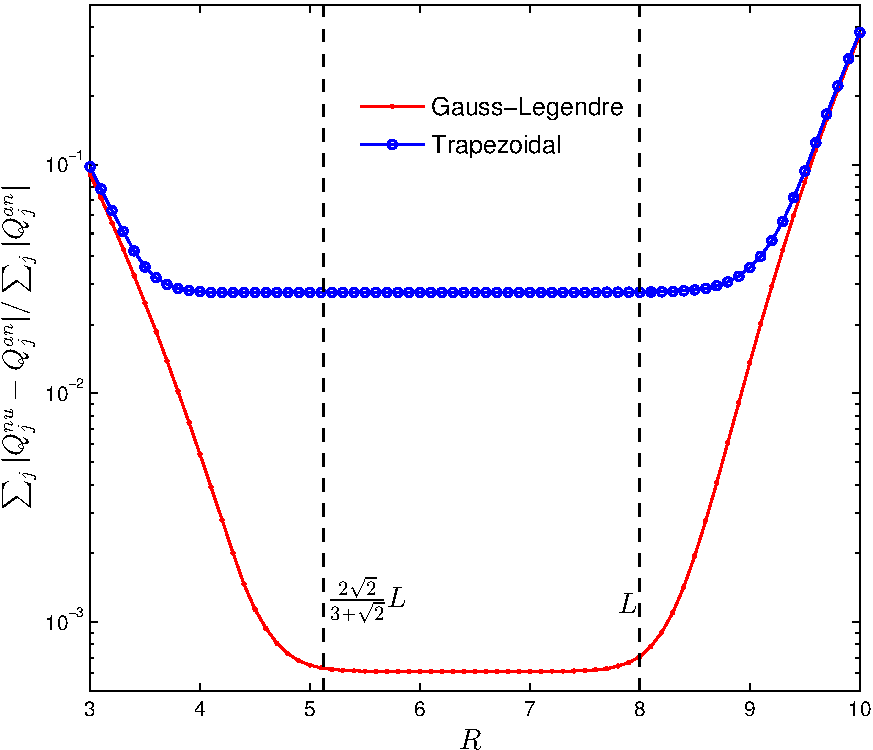
\includegraphics[width=7.5cm]{Chapter4/IMG/error_coll.pdf}
	\caption{
		The relative error versus the truncation radius $R$. Parameters are $L=8, N=48$, and $M=7$. The Gauss-Legendre quadrature is used in the approximation of the kernel mode.
	}
	\label{test_R}
\end{figure}


The integration of Eq.~\eqref{Boltzmann_homogeneous} with respect to $t$ will introduce some numerical error. In order to assess how accurately the FSM can approximate the Boltzmann collision operator, we compare $Q^{nu}$, the numerical approximation of $Q$, to the analytical solution $Q^{an}$, which is calculated by
\begin{equation}
Q^{an}(\bm{v})=\frac{f(\Delta{t},\bm{v})-f(0,\bm{v})}{\Delta{t}},
\end{equation}
with $\Delta{t}$=1.0E-5 (which is far smaller than the characteristic relaxation time $\text{Kn}'$). The following two factors affect the accuracy:
\begin{itemize}
	\item $N$, which decides the accuracy of the spectrum $\hat{f}$ of VDF;
	\item $M$, which determines how accurately we approximate Eq.~\eqref{kernel_mode2}.
\end{itemize}

The influence of $M$ is analyzed as follows. For simplicity, let us ignore $\xi_{\bm{m}}$ and $\varphi$ in Eq.~\eqref{kernel_mode2}. Notice that $\phi_{\alpha+\gamma}$ is a decaying-oscillating function with the quasi-period $2\pi/R$ (see Eq.~\eqref{int_res} and Fig.~\ref{phi_psi}). Then, for a fixed value of $\xi_{\bm{l}}$, the integral kernel in Eq.~\eqref{kernel_mode2} oscillates $R|\xi_{\bm{l}}|/\pi$ times as $\theta$ varies from 0 to $\pi$. In the worst case ($\xi_{\bm{l}}\rightarrow{}N\pi/2L$), it oscillates $O(N)$ times. This implies that $M$ should be $O(N)$. In practical calculations, however, $M$ can be far less than $N$ because, if the VDF has a support $S$, its spectrum has a support $1/S\sim{1/R}$. Within this support, the integral kernel in Eq.~\eqref{kernel_mode2} oscillates only a few times, and hence a small value of $M$ can lead to accurate result.


\begin{figure}[t]
	\centering
	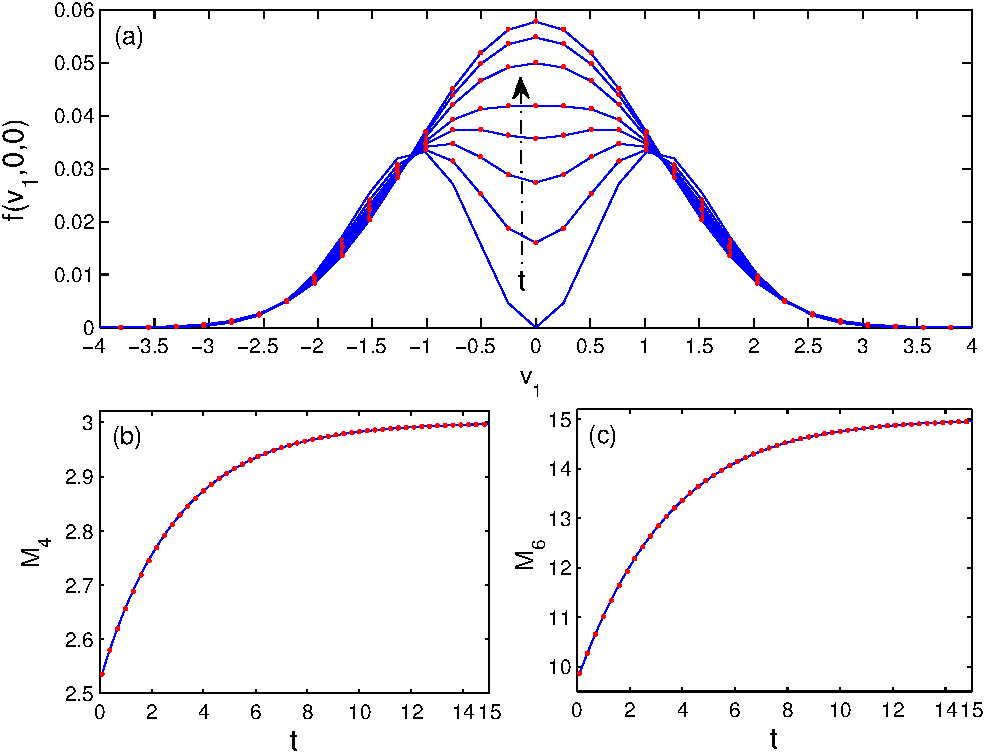
\includegraphics[width=11cm]{Chapter4/IMG/test11.pdf}
	\caption{
		(a) Evolution of $f(v_1,0,0)$ of space-homogeneous Maxwell molecules, from the initial condition~\eqref{initial_2}. From bottom to top (near $v_1=0$), the time corresponding to each line is $0, 0.5, 1, 1.5, 2, 3, 4$, and $5$. (b) and (c) Evolution of the fourth- and sixth-order moments, respectively. Solid lines: numerical result. Dots: analytical solution. Other parameters used in the numerical simulation are: $L=8, R=6$, $N=64$, and $M=5$ with Eq.~\eqref{kernel_FSM_mode}.  
	}
	\label{test2}
\end{figure}



We vary the values of $N$ and $M$ to see their influence on the numerical accuracy; the results are tabulated in Table~\ref{table_coll}. When $N=16$, the relative error is large because the resolution of VDF is not high enough so that a large error exists in the spectrum $\hat{f}$. As $N$ increases to 24, the error is reduced by one order of magnitude. When the trapezoidal rule is used, the error mainly comes from the approximation of Eq.~\eqref{kernel_mode2}, which decays at $O(M^{-2})$ when $N$ is fixed. When $M$ is fixed, the numerical accuracy does not improve when $N\ge32$. If we increase the value of $M$ by a factor of 2 when the value of $N$ is increased by the same factor, we find that the spectral accuracy of FSM is roughly maintained. When Eq.~\eqref{kernel_mode2} is approximated by the Gauss-Legendre quadrature, the spectral accuracy is clearly seen for $N\le32$ and $M\ge6$. When $N>32$, if $M$ is increased linearly with $N$, spectral accuracy is maintained. For example, if we choose the minimum error between $6\le{}M\le12$ for each $N$, the order of accuracy is 8.1 when $N$ increases from 16 to 24; 13.5 when $N$ increases from 24 to 32; and 8.9 when $N$ increases from 32 to 48.  Thus, in general, the approximation of Eq.~\eqref{kernel_mode2} by the Gauss-Legendre quadrature is better than that by the trapezoidal rule.




We now fix the values of $N$ and $M$ to check the influence of $R$ on the accuracy, see Eq.~\eqref{velocity_truncation}. Fig.~\ref{test_R} indicates that $R$ cannot be smaller than $2\sqrt{2}L/(3+\sqrt{2})$, which is roughly $\sqrt{2}$ times the support of VDF; otherwise, some collisions will be ignored in the truncated collision operator. Also, $R$ cannot be larger than the size of velocity domain, otherwise the aliasing error may destroy accuracy.

%
%\begin{figure}[t]
%	\centering
%	\includegraphics[width=10cm]{error_time.pdf}
%	\caption{ 
%		(a) Error $(\sum_{\bm{j}}|f^{nu}-f|^2/\sum_{\bm{j}}|f|^2)^{1/2}$ in the VDF, (b) error in the fourth-order moment $|M_4^{nu}-M_4|/M_4$, (c) error in the sixth-order moment $|M_6^{nu}-M_6|/M_6$, and (d) error in the energy $|(p^{nu}_{xx}+p^{nu}_{yy}+p^{nu}_{zz})/6-1|$ vs time. Solid and dashed lines are the results using Eq.~\eqref{kernel_FSM_modee} with $N=24$ and $N=32$, respectively, while dotted lines are the results using Eq.~\eqref{kernel_FSM_mode} with $N=32$. Other parameters are $L=8,R=6$, and $M=7$.
%	}
%	\label{test_time}
%\end{figure}


Next, we demonstrate the accuracy of FSM in the homogeneous relaxation, where Eq.~\eqref{Boltzmann_homogeneous} is solved by the Euler forward method with a time step of $0.001$. Figure~\ref{test2} depicts the evolution of VDF, as well as the fourth- and sixth-order moments. Excellent agreement is found between the numerical and analytical solutions, even when Eq.~\eqref{kernel_mode2} is approximated by the trapezoidal rule with $M=5$. 

%Figure~\ref{test_time} shows the numerical errors in the VDF, the fourth- and sixth-order moments, and energy as functions of time. When Eq.~\eqref{kernel_mode2} is approximated by the Gauss-Legendre quadrature, the numerical error with $N=32$ is one order of magnitude smaller than that with $N=24$. Also, the accuracy of the results with $N=24$ is even better than that with $N=32$ when Eq.~\eqref{kernel_mode2} is approximated by the trapezoidal rule. These results agree with what we found in Table~\ref{table_coll}. 

%Furthermore, we find that the use of Lagrangian multiplier method does not affect the numerical accuracy. This could be explained as follows: from Fig.~\ref{test_time}(a) and (d) we see that the error in energy is far smaller than the error in  VDF. Therefore, the correction in Eq.~\eqref{Lagrangian1} is negligible, which ensures conservation. 
%
%Comparing the kernel mode~\eqref{kernel_FSM_mode} with those in Refs.~\cite{Mouhot2006,Filbet2006,Hu2012}, the term $\sin\theta_p$ is missed in Refs.~\cite{Mouhot2006,Filbet2006} and an additional term $\sin\theta_2$ is added in Eq.~\eqref{psi_FSM_expression} in Ref.~\cite{Hu2012}. We have carried out numerical simulations using these kernel modes and found that none of them can accurately capture the evolution of VDF.


\begin{figure}[t]
\centering 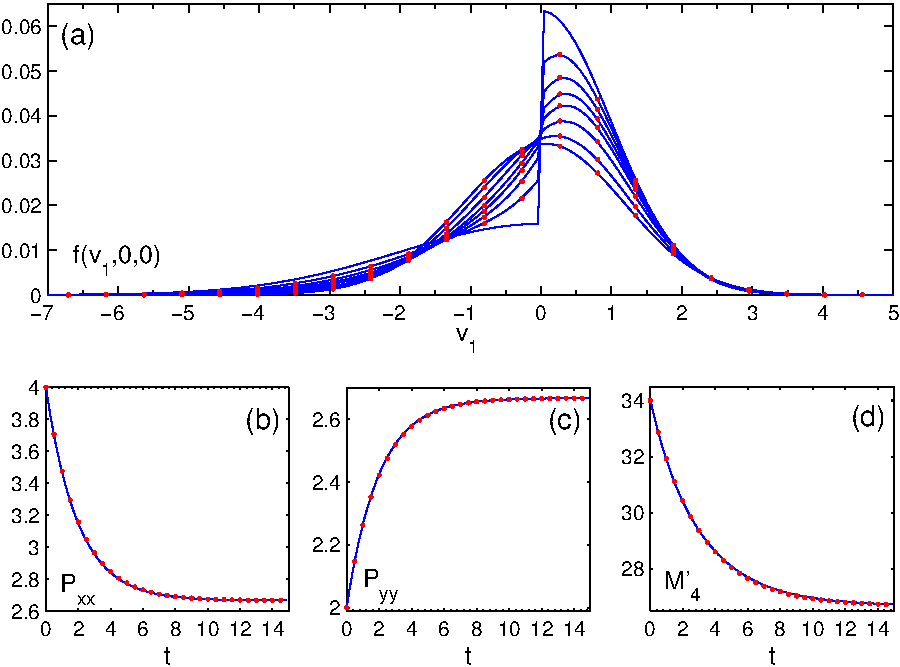
\includegraphics[width=9cm]{Chapter4/IMG/test3_2.pdf}\\
\vskip 0.3cm 
\centering 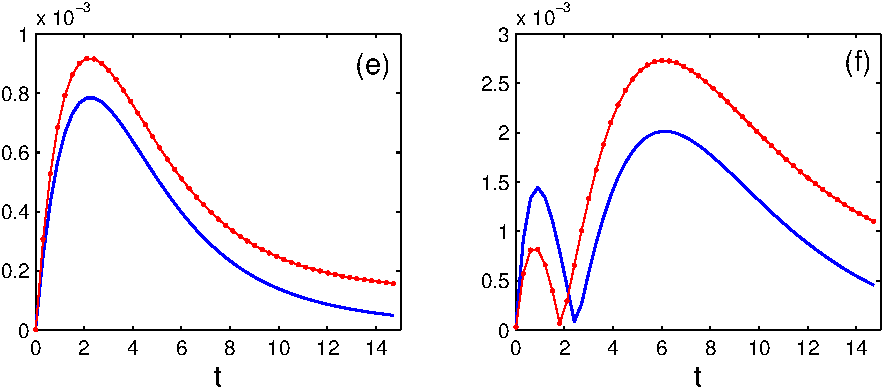
\includegraphics[width=9cm]{Chapter4/IMG/test_error3.pdf}
\caption{ 
	(a) Evolution of the VDF when the initial VDF at $v_1=+0$ is four times larger than at $v_1=-0$. From top to bottom (at $v_1>0$), the times corresponding to the lines are $t=0, 0.5, 1, 1.5, 2, 3, 5$, and $9$, respectively. (b-d) Evolution of the second- and fourth-order moments. Relative error (e) $|p^{nu}_{xx}-p_{xx}|/p_{xx}$ and (f) $|M^{'nu}_{4}-M_{4}^{'}|/M_{4}^{'}$ when $N=42$. Dots are the numerical results when $N_1=N_2=N_3=42$, solid lines in (a), (e), and (f) are the numerical results with $N_1=256, N_2,N_3=42$, while solid lines in (b-d) are analytical solutions. Other parameters are $L_v=11$, $R=2\sqrt{2}L_v/(3+\sqrt{2})$, and $M=5$ with Eq.~\eqref{kernel_FSM_mode}.
} 
\label{test3}
\end{figure}


\subsection{Discontinuous velocity distribution function}

The initial VDF used in the preceding case is smooth, where the spectral accuracy of FSM can be proven analytically~\cite{Mouhot2006}. Now we consider the case where the initial VDF is not smooth, but has an abrupt jump at $v_1=0$:
\begin{equation}\label{initial_3}
f(\bm{v},t=0)=\frac{1}{3(2\pi)^{3/2}}
\begin{cases}
4\exp\left(-\frac{{v^2}}{2}\right) , & v_1\ge0,  \\
\exp\left(-\frac{v_1^2}{8}-\frac{v_2^2+v_3^2}{2}\right), &  v_1<0.
\end{cases}
\end{equation}

Although the analytical solution for the VDF cannot be obtained, it can be shown analytically that the evolution of the second- and fourth-order moments is given by
\begin{equation}\label{initial_33}
\begin{aligned}[b]
  P_{xx} = \frac{4}{3}\exp\left(-\frac{t}{2}\right)+\frac{8}{3}, \\
  P_{yy} = -\frac{2}{3}\exp\left(-\frac{t}{2}\right)+\frac{8}{3}, \\
  M'_{4} = \int fv^4d\bm{v}=\frac{22}{3}\exp\left(-\frac{t}{3}\right)+\frac{80}{3}.
 \end{aligned}
\end{equation}


Figure~\ref{test3} demonstrates that the FSM can accurately capture the evolution of second- and fourth-order moments, even when the initial VDF has a large jump at $v_1=0$. Also, no Gibbs oscillation has been observed in the central region of VDF where the abrupt jump exists; only in the tails do we find small Gibbs oscillations. This is because the convolution in the Boltzmann collision operator can smear out discontinuities.


\begin{figure}[t]
	\centering
	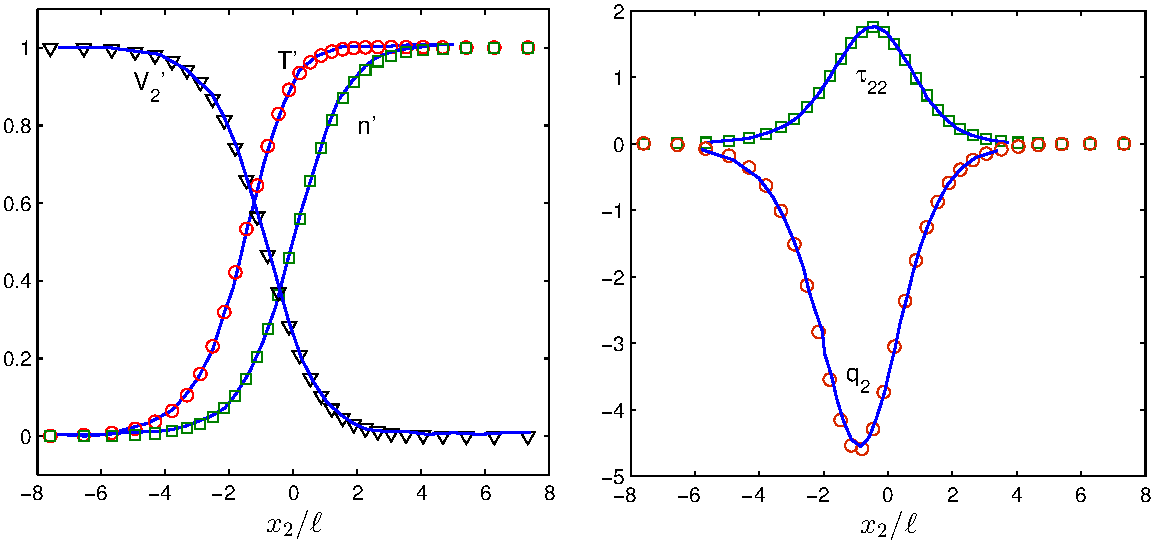
\includegraphics[scale=0.7]{Chapter4/IMG/shock_hard_M3.pdf}
	\caption{
		The structure of normal shock wave when $\text{Ma}=3$, where the reduced macroscopic quantity $\mathcal{M}=\rho, u, T$ is normalized as ${(\mathcal{M}-\mathcal{M}_u)/(\mathcal{M}_d-\mathcal{M}_u)}$, with the subscripts ${u}$ and ${d}$ represent upstream and downstream, respectively. Solid lines are the results from Ref.~\cite{Ohwada1993}, while symbols are our FSM results. 
	}
	\label{shock_Ohwada}
\end{figure}

\section{Accuracy in inhomogeneous problems}\label{CIS_first_time}


The Boltzmann equation is solved by the CIS~\eqref{iteration2}, where the spatial derivative ${\partial {f}}/{\partial\bm{x}}$ is approximated by the second-order upwind scheme.

\index{finite-difference}
\index{upwind}

%In the following calculations, it is found that the use of $M=5$ generates satisfactory results. We use the trapezoidal rule to approximate the kernel mode~\eqref{kernel_mode2}, since for $M=5$ it has almost the same accuracy as that of Gauss-Legendre quadrature but with about 25\% decrease in computational time.

\subsection{Normal shock waves}
\index{shock wave}

\begin{figure}[t]
	\centering
	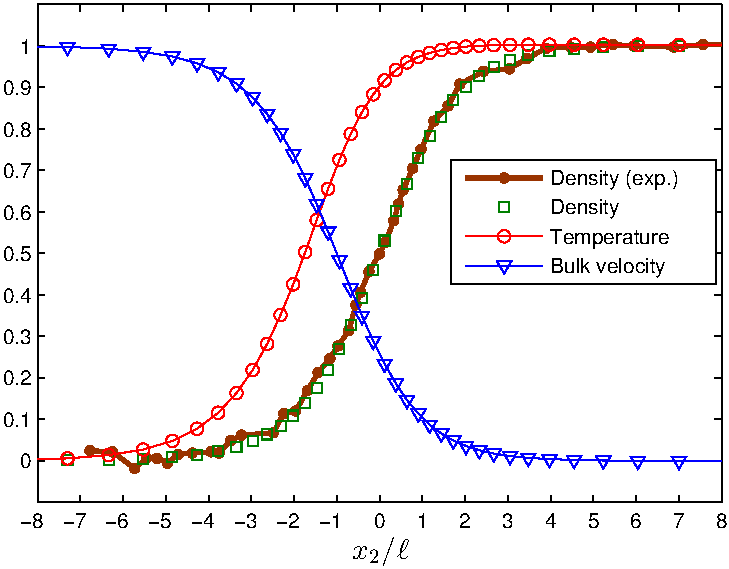
\includegraphics[width=7cm]{Chapter4/IMG/shock_exp.pdf}
	\caption{
		Reduced number density, temperature, and bulk velocity for the normal shock wave of $\text{Ma}=2.80$ in the argon gas, with the upstream temperature of $298\pm3$~K. The experimental density is obtained from Ref.~\cite{Kowalczyk2008}. Numerical parameters are the same as those in Fig.~\ref{shock_Ohwada}.
	}
	\label{shock_exp}
\end{figure}

The normal shock wave problem is ideal for testing the accuracy of FSM in capturing strong rarefaction effects, since this is a one-dimensional problem where the boundary effects are absent. The structure of the planar shock wave varies in the $x_2$ direction. The flow is uniform at the upstream ($x_2=-\infty$) and downstream ($x_2=\infty$) ends. The upstream molecule number density, temperature, and Mach number are denoted by $n_0$, $T_0$, and $\text{Ma}$, respectively, while those of the downstream end is determined through the Rankine-Hugoniot relations: \index{Rankine-Hugoniot relations}
\begin{equation*}%\label{rankine}
\begin{aligned}[b]
n_d=\frac{4\text{Ma}^2}{\text{Ma}^2+3}, \quad
u_d=\sqrt{\frac{5}{96}}\frac{\text{Ma}^2+3}{\text{Ma}},\quad
T_d=\frac{(5\text{Ma}^2-1)(\text{Ma}^2+3)}{16\text{Ma}^2},
\end{aligned}
\end{equation*}
hence the normalized VDF at the upstream end is
\begin{equation}\label{shock_upstream}
    {f}=\frac{1}{{\pi}^{3/2}}\exp\left[-{v}_1^2-
    \left({v}_2-\sqrt{\frac{5}{6}}\text{Ma}\right)^2-{v}_3^2\right],
\end{equation}
and that at the downstream end is
\begin{equation}\label{down_upstream}
    {f}=\frac{n_d}{(\pi{T_d})^{3/2}}\exp\left[-\frac{{v}_1^2+
    ({v}_2-u_d)^2+{v}_3^2}{T_d}\right].
\end{equation}


\subsubsection{Hard-sphere potential}
\index{numerical kernel method}

We first consider the shock wave in a gas of HS molecules. Ohwada solved the Boltzmann equation by means of the numerical kernel method~\cite{Ohwada1993}. For comparison, 
we set $L$ to be the mean free path in the upstream part
\begin{equation}
\lambda_0=\frac{16}{5\pi}\sqrt{\frac{\pi}{2mk_BT_0}}
\frac{\mu}{n_0},
\end{equation} 
and $\text{Kn}=5\pi/16$. Figure~\ref{shock_Ohwada} shows the shock wave structure for a Mach number of 3. In FSM the velocity domain $[-10,10]^3$ is uniformly divided into $42\times42\times42$ grid points, and $M=5$. It can be seen that the two deterministic numerical methods for the Boltzmann equation give identical results.


\begin{figure}[t]
	\centering
	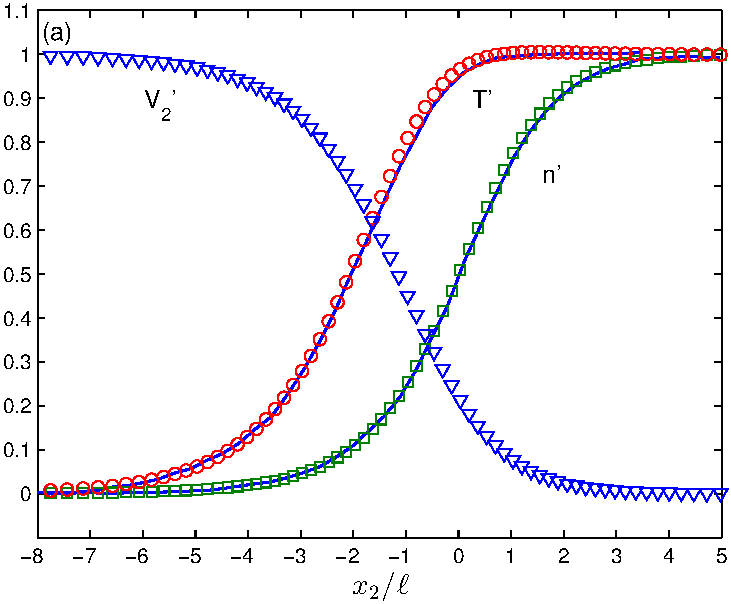
\includegraphics[width=6cm]{Chapter4/IMG/shock_M5_compare2.pdf} \hskip 0.5cm
	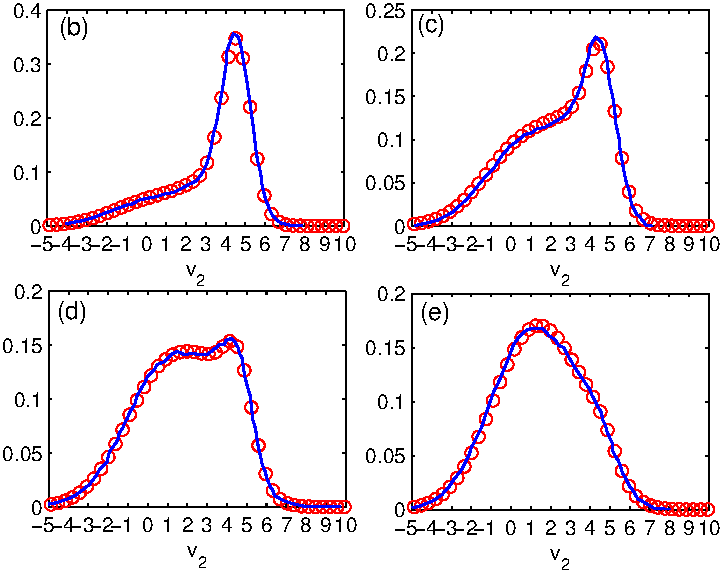
\includegraphics[width=6.2cm]{Chapter4/IMG/shock_LJ_M5_dist.pdf}
	\caption{
		(a) Reduced molecular number density, temperature, and bulk velocity for the normal shock with $\text{Ma}=5$ in argon gas (Lennard-Jones potential). \index{velocity distribution function!marginal}The marginal VDF $\int\int fdv_1dv_3/n$ vs $v_2$ is presented when the reduced density is (b) $0.151$, (c) $0.350$, (d) $0.511$, and (e) $0.759$. Solid lines are the results from Ref.~\cite{Valentini2009}, while symbols are our results from the FSM. The velocity domain $[-18,18]^3$ is divided into $42\times84\times42$ grid points. }
	\label{shock_MD}
\end{figure}



\subsubsection{Lennard-Jones potential}

We then consider argon with the Lennard-Jones \index{Lennard-Jones potential} potential. To compare with experimental data~\cite{Kowalczyk2008}, we set the upstream temperature to be $T_0$ = 298 K, $L$ to be the mean free path in the upstream part,
and hence $\text{Kn}=5\pi/16$ in Eq.~\eqref{LJ_kernel}. Good agreement between the numerical and experimental density profiles is seen in Fig.~\ref{shock_exp}. The agreement is due to the fact that we have correctly incorporated the shear viscosity of argon into the collision kernel, shown in Eq.~\eqref{kernel_spectral}. 


\index{molecular dynamics simulation}
Finally, we solve the Boltzmann equation for argon with the Lennard-Jones potential~\eqref{Lennard_Jones_chapter} and compare our results with molecular dynamics simulation~\cite{Valentini2009}. For comparison, we set the upstream temperature to be $T_0$ = 300 K, $L$ to be the mean free path in the upstream part and $\text{Kn}=5\pi/16$. Fig.~\ref{shock_MD} shows the shock wave structure for Mach number of 5, as well as the marginal VDFs. The FSM produces nearly the same results as the molecular dynamics simulation, not only in macroscopic quantities, but also in mesoscopic VDFs. Note that in this case the downstream temperature is about 2600~K. The excellent agreement with molecular dynamics data illustrates that the collision kernel~\eqref{LJ_kernel} for the Lennard-Jones potential works well in this temperature range.


\subsection{Force-driven Poiseuille flows}\label{force_driven}
%\index{Fourier flow}
%\index{Couette flow}
\index{Poiseuille flow}


Consider a rarefied monatomic gas between two parallel infinite plates located at $x_2=L/2$ and $x_2=-L/2$. The walls are stationary, and the temperature is kept at $T_0$. The gas is subject to a uniform external acceleration $a_1$ in the $x_1$ direction; the acceleration term $\bm{a}\cdot\partial f/\partial \bm{v}$ is calculated according to the Fourier transform derivative theorem. Diffuse boundary condition is employed to account for the wall effects.


\begin{figure}[t]
	\centering
	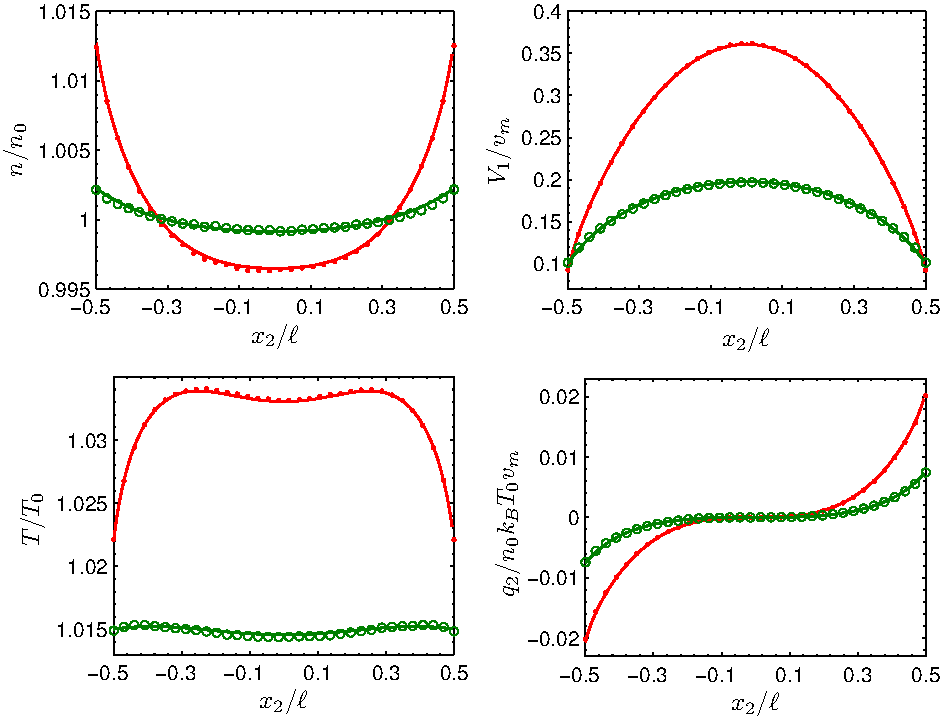
\includegraphics[width=12cm]{Chapter4/IMG/poiseuille_hard.pdf}
	\caption{
		The density, velocity, temperature, and heat flux in the force-driven Poiseuille flow of HS molecules when $\text{Kn}=0.1$ (dots) and $\text{Kn}=0.5$ (open circles). Solid lines are FSM results, while symbols are DSMC results~\cite{Meng2013JCP}.
	}
	\label{poiseuille_fig}
\end{figure}



We solve the discretized Boltzmann equation by the CIS. At the $(k+1)$-th iteration step, the VDF at the wall (entering the cavity) is determined according to the diffuse boundary condition, using the VDF at the same position at the previous iteration step:
\begin{equation}\label{wall_boundary}
\begin{aligned}[b]
{f}^{(k+1)}=&\frac{{n}}{{\pi}^{3/2}}\exp[-({v}_1+{u}_w)^2-{v}_2^2-{v}_3^2],
\ \ \ \operatorname{for} \ {v}_2\le0, \\
{n}=&2\sqrt{\pi}\int_{{v}_2<0}
{v}_2
{f}^{(k)}({x}_2=-0.5,{v})d\bm{v},
\end{aligned}
\end{equation}
This numerical scheme is efficient when the Knudsen number is not small. However, the total mass is not conserved since the mass flux entering the computational domain at the $(k+1)$-th step (which is equal to that leaving the computational domain at the $k$-th step) is not equal to that leaving the computational domain at the $(k+1)$-th step. To overcome this, at the end of each iteration, the VDF is re-scaled so that the total mass is conserved~\cite{Mieussens2004}. Physically, when the average molecular number density $n_0$ and the intermolecular potential are known, the stationary state will be uniquely determined. 



%
%\begin{figure}[t]
%	\centering
%	\includegraphics[width=5.5cm]{lid_arg_Knvhs01u.pdf}
%	\quad
%	\includegraphics[width=5.5cm]{lid_arg_Knvhs01q.pdf}\\
%	\vskip 0.2cm
%	\includegraphics[width=5.5cm]{lid_arg_Knvhs1u.pdf}
%	\quad
%	\includegraphics[width=5.5cm]{lid_arg_Knvhs1q.pdf}
%	\\
%	\vskip 0.2cm
%	\includegraphics[width=5.5cm]{lid_arg_Knvhs10u.pdf}
%	\quad
%	\includegraphics[width=5.5cm]{lid_arg_Knvhs10q.pdf}
%	\caption{Temperature contours and streamlines (velocity: first column; heat flux: second column) in the lid-driven cavity flow of argon gas. From top to bottom, the Knudsen number $\text{Kn}_{vhs}$ defined in Eq.~\eqref{Kn_VHS} in each column is 0.1, 1 and 10, respectively.  Here and after, the abscissa represents the $x_1$-axis, while the ordinate represents the $x_2$-axis.  } 
%	\label{lid}
%\end{figure}

Consider HS molecules when $\text{Kn}=0.1$ and $0.5$. The normalized acceleration is $0.11$ and the wall temperature is $T_0$=273~K. The spatial region (halved due to the symmetry) is divided into $50$ unequally spaced cells with more cells near the boundary. The maximum velocity is at $L_v=6$, and there are 32 velocity mesh points in each direction. The numerical results are depicted in Fig.~\ref{poiseuille_fig}, where good agreements can be found. Note that in this case, the temperature profile has double peaks, which is in sharp contrast with the parabolic profiles predicted by the NSF equations~\cite{Zheng2002}. 

%
%\subsection{Lid-driven cavity flow}
%
%
%
%
%The lid-driven cavity flow is a canonical problem in rarefied gas flows, since it clearly shows the non-equilibrium phenomena where the heat flux is from low-temperature region to high-temperature region, see Fig.~\ref{lid}. The DSMC is extremely time-consuming (i.e., takes about 1000 hours) to find the steady-state solution due to the low velocity near the bottom plate~\citep{John2010,John2011}. Even when the velocity of the moving upper lid is so small that the linearized Boltzmann equation can be applied, the low-noise DSMC method~\citep{Radtke2011} takes more than 1 day to achieve reasonably resolved results when the Knudsen number based on the MFP of variable HS model is $\text{Kn}_{vhs}=0.1$. 
%
%%\begin{figure}[t]
%%	\centering
%%	\includegraphics[scale=0.4]{lid_central_horizontal.pdf}
%%	\includegraphics[scale=0.4]{lid_central_vertical.pdf}\\
%%	\includegraphics[scale=0.4]{lidT.pdf}
%%	\caption{
%%		(Top) Comparisons of the velocity and heat flux profiles between argon and HS gases in the lid-driven cavity flow. (Left) At $x_2=0.5$ and (right) At $x_1=0.5$. Solid (or dashed) lines are the results for argon with $\text{Kn}_{vhs}=0.1$ (or 10), while  circles (or stars) are the results for the HS gas with $\text{Kn}_{vhs}=0.132$ (or 13.2). (Bottom) Comparisons of temperature profiles between argon and HS gases in the lid-driven cavity flow. Filled (open) markers: $x_1=0.5$ $(x_2=0.5)$. 
%%	} 
%%	\label{lidvqt}
%%\end{figure}
%
%We solve this problem (for argon gas, the upper lid velocity of 50~m/s, and a wall temperature of 273~K) in a $51\times51$ nonuniform spatial grid (with most of the grid points located in the vicinity of walls): 
%\begin{equation}\label{spatial_d}
%x=(10-15s+6s^2)s^3, 
%\end{equation}
%with $s=(0,1,\cdots,N_s)/N_s$. The minimum length of the spatial cell is $7.8\times10^{-5}$, while the maximum is 0.0375. For $\text{Kn}_{vhs}=0.1$ and 1,  $32\times32\times12$ grid points in velocity space are used, while for $\text{Kn}_{vhs}=10$, there are $64\times64\times12$ velocity grid points, with most of the grid points located in $v_1,v_2\sim0$ to capture the discontinuities in VDF, see Eq.~\eqref{nonuniform_v}. The number of uniform frequency components is $32\times32\times24$. The Boltzmann collision operator is approximated by the FSM with $M=6$. 
%
%%\begin{equation}
%%||\epsilon||_2=max\left\{\sqrt{\frac{\int|u_1^{k+1}-u_1^k|^2dx_1dx_2}{\int|u_1^k|^2dx_1dx_2}},\sqrt{\frac{\int|u_2^{k+1}-u_2^k|^2dx_1dx_2}{\int|u_2^k|^2dx_1dx_2}}\right\},
%%\end{equation} 
%
%The convergence rate of our iterative scheme is proportional to the Knudsen number. For $\text{Kn}_{vhs}=0.1$ and 1, starting from the global equilibrium state, the FSM takes 110 and 14 minutes, respectively, to produce a converged solution,  when the relative error in flow velocity between two consecutive iteration steps, is less than $10^{-5}$.
%
%Fig.~\ref{lid} shows the calculated temperature contours and streamlines in the lid-driven cavity flow of argon gas with diffuse boundary conditions. Compared to DSMC, these solutions are free of noise. We have also simulated the flow of a HS gas, with the same values of the normalized wall velocity and shear viscosity (the Knudsen number $\text{Kn}$ are the same, but $\text{Kn}_{vhs}$ are different). Comparisons of the velocity, temperature, and heat flux  between the two inverse power-law molecular models demonstrate that the molecular model (reflected in terms of the collision kernel) has little influence on the flow pattern in this case, see Ref.~\cite{lei_Jfm}.




\subsection{Thermal transpiration}\label{chapter_FSM_tc}

\begin{figure}[p]
	\centering
	{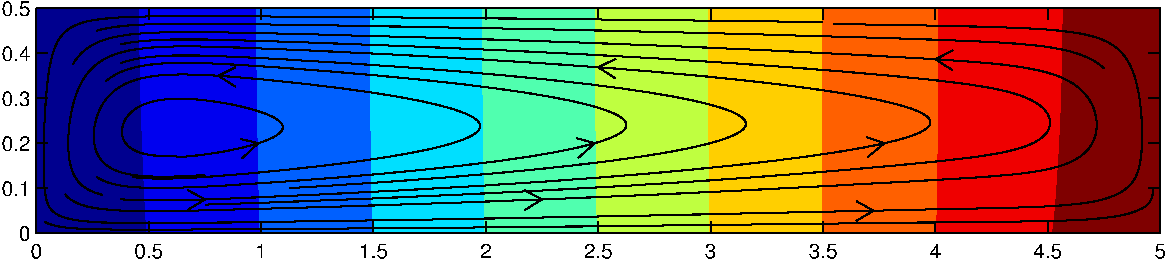
\includegraphics[width=11cm]{Chapter4/IMG/Tc008.pdf}}\\
	{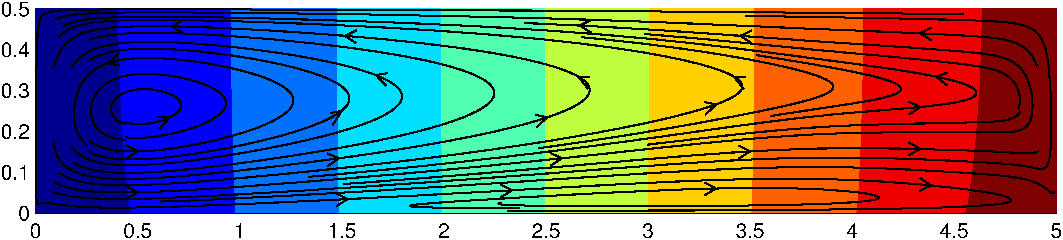
\includegraphics[width=11cm]{Chapter4/IMG/Tc02.pdf}}\\
	{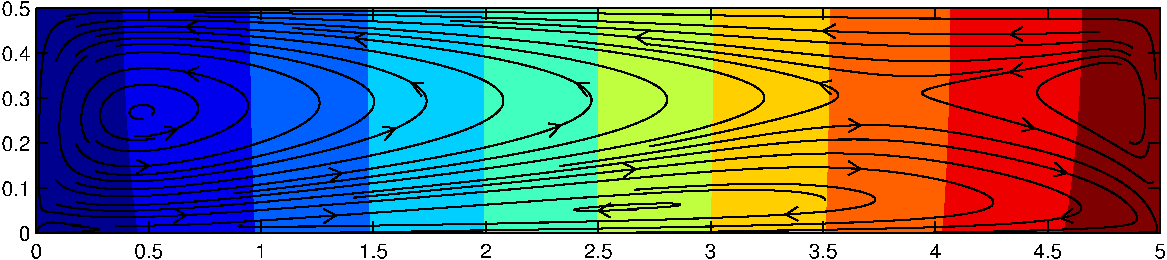
\includegraphics[width=11cm]{Chapter4/IMG/Tc025.pdf}}\\
	{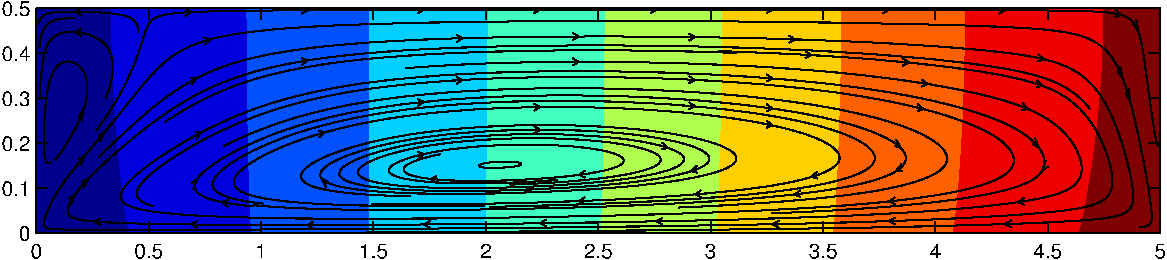
\includegraphics[width=11cm]{Chapter4/IMG/Tc06.pdf}}\\
	{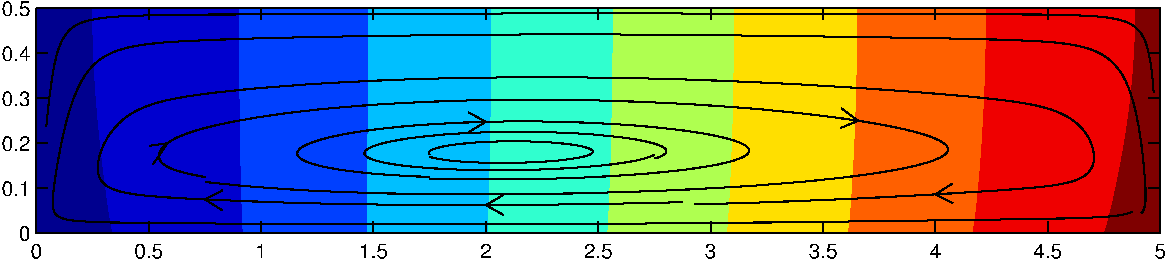
\includegraphics[width=11cm]{Chapter4/IMG/Tc2.pdf}}\\
	{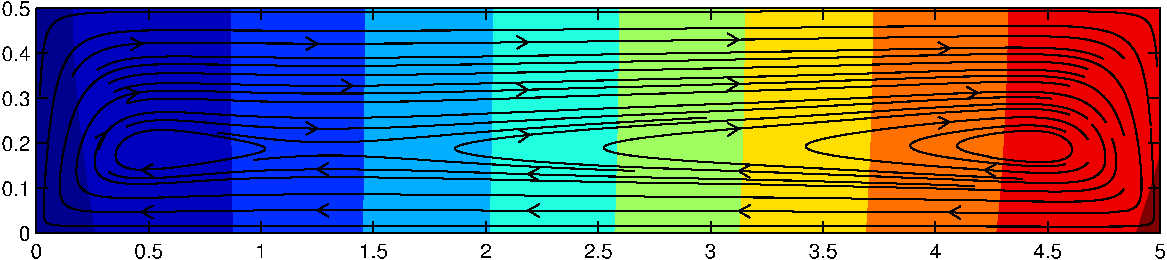
\includegraphics[width=11cm]{Chapter4/IMG/Tc10.pdf}}
	\caption{Temperature contours and velocity streamlines in the thermal transpiration of argon gas within a closed rectangular channel (only the down half domain is shown). In each figure, from left to right, the dimensionless temperature of each contour is $1+0.1i$, where $i=1,2,\cdots,9$. From the top to bottom, $\text{Kn}=0.08$, 0.2, 0.25, 0.6, 2, and 10, respectively. } 
	\label{thermal_creep_channel}
\end{figure}


Consider the thermal transpiration in a 2D closed rectangular channel with a length-to-width ratio of 5. The temperature at the right side is set to be twice that of the left side, while the temperature of the top and bottom walls varies linearly along the channel. Using the mean density, the temperature of the left wall, and the channel width, the Knudsen number is set to be $\text{Kn}=0.08$, 0.2, 0.25, 0.6, 2, and 10. 

Figure~\ref{thermal_creep_channel} presents the  streamlines and temperature distributions inside the channel for the flow of argon gas. Due to symmetry, only half of the spatial domain is shown. At $\text{Kn}=0.08$, the gas flows from the cold region to the hot region along the bottom wall, and returns in the central region. At $\text{Kn}=0.2$, the flow still moves from hot to cold in the central region, however, near the lower wall the flow moves towards the hot region when $x_1<2$ and towards the cold region for at $x_1>2$, i.e., a circulation emerges near the lower corner of the domain. At $\text{Kn}=0.25$, the circulation near the lower wall grows, which divides the flow in the central region into two circulation zones. The lower circulation zone keeps expanding, and pushes the other two circulations in the central region towards the left and right boundaries, as $\text{Kn}$ increases. At $\text{Kn}=0.6$, the flow direction is reversed (as compared to that when $\text{Kn}=0.08$) and only one circulation zone remains near the left wall. The reversal of flow direction persists but the circulations near the left wall gradually disappear as the Knudsen number increases further, for instance, to $\text{Kn}=2$. By $\text{Kn}=10$, the gas near the bottom wall moves from hot to cold, and two clockwise circulations emerge near the left and right sides. Finally, when the flow enters the free molecular regime, the streamline pattern does not change, but the velocity magnitudes are proportional to $1/\text{Kn}$. The magnitudes of density, pressure, and temperature, however, remain unchanged irrespective of the Knudsen number~\cite{lei_Jfm}.

%\begin{figure}
%	\centering
%	{\includegraphics[width=6cm]{tc_free.pdf}}
%	\hskip 0.8cm
%	{\includegraphics[width=5.4cm]{scale_velocity.pdf}}
%	\caption{(Left) The average horizontal velocity varying with $\text{Kn}$ in thermal transpiration inside the closed rectangular channel, in the free molecular regime. In this double logarithmic diagram, the three lines have a slope of 1, demonstrating that the velocity magnitude is proportional to $1/Kn$. (Right) Examples of the linear scalability of the horizontal velocity at $x_1=1.4825$.  } 
%	\label{tc_free}
%\end{figure}

Comparison of the velocity profiles for different molecular models at the start and the end of the transition flow regime  are shown in Fig.~\ref{thermal_creep_v}; it can be seen that the molecular model (reflected in terms of the viscosity index) affects the velocity magnitudes significantly. 

\begin{figure}[t]
	\centering
	{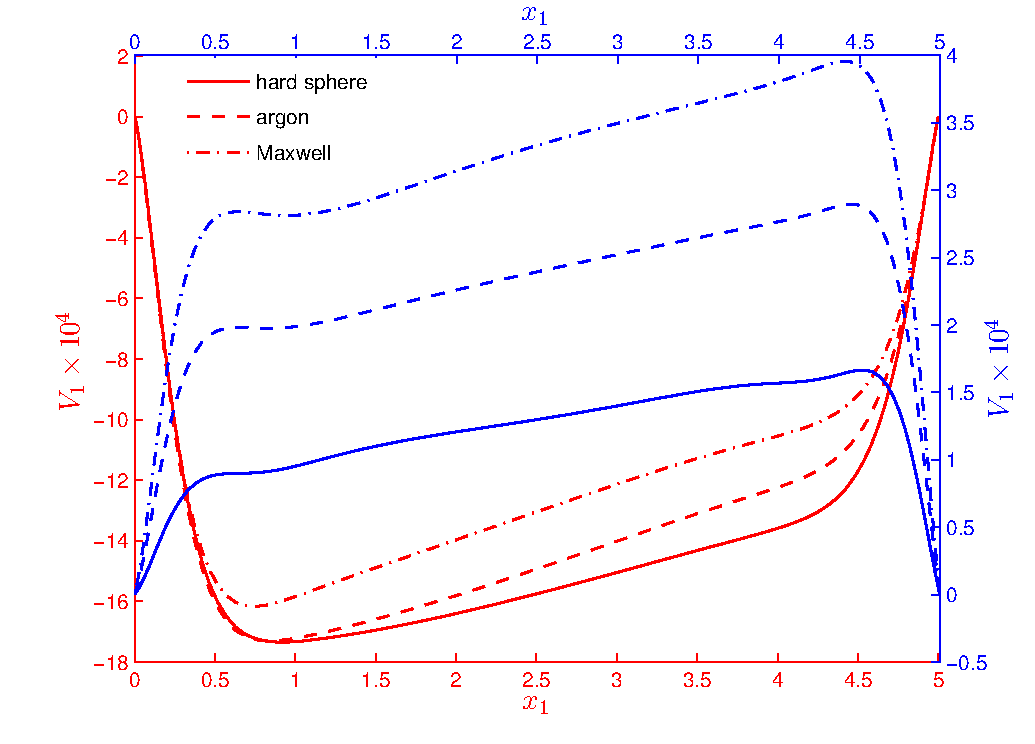
\includegraphics[width=6.5cm]{Chapter4/IMG/tch.pdf}}\hskip 0.4cm
	{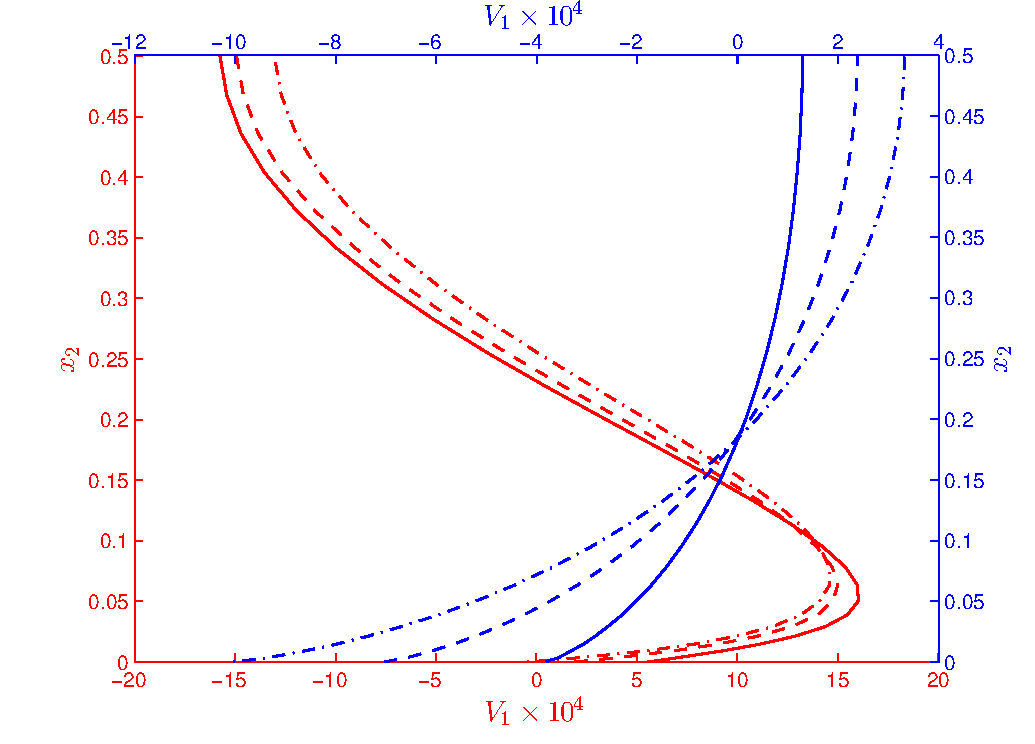
\includegraphics[width=6.5cm]{Chapter4/IMG/tcv.pdf}}
	\caption{Velocity profiles for thermal transpiration within a closed rectangular channel: (a) along the central horizontal line and (b) along the central vertical line. $\text{Kn}=0.08$ and $10$ are represented by the red and blue lines, respectively.} 
	\label{thermal_creep_v}
\end{figure}


%\begin{figure}[t]
%	\centering
%	{\includegraphics[width=8cm]{tc_compare-crop.pdf}}
%	\caption{Net velocity profiles obtained by linear superposition of the velocity profiles of Poiseuille and thermal transpirations between parallel plates, which result in zero mass flow rate. The walls are at $x_2=0$ and $x_2=1$ and the working gas is argon, where the inverse power-law model with $\omega=0.81$ is used.} 
%	\label{tc_mechanism}
%\end{figure}

%The flow patterns shown in Fig.~\ref{thermal_creep_channel} can be understood qualitatively as follows. Starting from the global equilibrium state, the temperature gradient drives the gas molecules to move from cold to hot (thermal transpiration). This process increases the pressure at the right side of the channel while decreasing the pressure at the left. Then, the pressure gradient causes the gas molecules to move to the left (Poiseuille flow). The steady state is reached when the effects of Poiseuille and thermal transpirations cancel each other out, that is, when the net mass flow rate across the lines perpendicular to the top and bottom walls is zero. The horizontal velocity profile can be analysed by assuming the wall temperature gradient to be small (i.e. the channel is long enough) so that the Boltzmann equation can be linearized. In this case, we can directly use the velocity profiles obtained in Sec.~\ref{pt}. Fig.~\ref{tc_mechanism} plots the net velocity profiles in the linear superposition of Poiseuille and thermal transpirations between parallel plates where the net mass flow rate is zero.  The flow velocities are normalised; in real problems, the horizontal velocity is given by (see the first paragraph in Sec.~\ref{tc_linear}):
%\begin{equation}\label{superposition}
%u_1=\beta_T\left\{u_1[h_T]-\frac{\mathcal{M}[h_T]}{\mathcal{M}[h_P]}u_1[h_P]\right\},
%\end{equation}
%where $\beta_T$ is the temperature gradient; in this case, it is about $1/5$.
%
%Now the horizontal velocity profiles in Fig.~\ref{tc_mechanism} can be used to explain the flow patterns in Fig.~\ref{thermal_creep_channel}. 
%From Fig.~\ref{tc_mechanism} we find that, when $\text{Kn}=\sqrt{\pi}/20$, the net horizontal velocity is positive when $x_2<0.25$ and negative otherwise, which agrees well with the flow pattern in Fig.~\ref{thermal_creep_channel}(a). Also, from Fig.~\ref{thermal_creep_v}(a) we find that, at $\text{Kn}=0.08$, $u_1(x_2=0.5)\simeq-0.0018$ near the left side of the channel, which is well predicted by equation~\eqref{superposition} when we choose $\text{Kn}=\sqrt{\pi}/20$ and $x_2=0.5$: $u_1(x_2=0.5)\simeq(-0.009)/5=-0.0018$. Furthermore, as $\text{Kn}$ increases, the magnitude of the horizontal velocity at $x_2=0.5$ decreases (Fig.~\ref{tc_mechanism}). This is in accordance with the horizontal velocity profiles shown in Fig.~\ref{thermal_creep_v}(a), where the velocity magnitude decreases as $x_1$ increases from 1 to 4, because the local Knudsen number increases along the channel as a result of increasing temperature  and decreasing particle number density.  When $\text{Kn}=\sqrt{\pi}/10$ (and $\sqrt{\pi}/8$), the net horizontal velocity in Figure~\ref{tc_mechanism} is positive when $0.26>x_2>0.009$ (and $0.28>x_2>0.023$) and negative otherwise. This explains the flow patterns at the right side of the channel, as shown in Figure~\ref{thermal_creep_channel}(b). As $\text{Kn}$ increases, the extent of the region near the bottom wall where the velocity is negative increases (Figure~\ref{tc_mechanism}), so that the circulation near the bottom wall in Figure~\ref{thermal_creep_channel}(c) is larger than that in Figure~\ref{thermal_creep_channel}(b). When $\text{Kn}$ increases above a critical value of around $\sqrt{\pi}/5$, the horizontal velocity in Figure~\ref{tc_mechanism} is negative when $x_2$ is smaller than some fixed value $x_{2c}$ and positive otherwise. In this case, the flow direction is completely reversed in comparison with that at small Knudsen numbers.  When $\text{Kn}>\sqrt{\pi}/2$,  the fixed value is $x_{2c}=0.2$. In Figure~\ref{thermal_creep_channel}(d-f), we see that the gas moves from left to right if $x_2<0.2$, and moves right to left if $x_2>0.2$. 

%\begin{figure}[t]
%	\centering
%	{\includegraphics[width=10cm]{flow_pattern.pdf}}
%	\caption{Thermal transpiration patterns of the argon gas (inverse power-law model with $\omega=0.81$) in the free molecular regime at different values of length-to-height ratio $A$. (a) $A=0.25$, (b) $A=0.5$, (c) $A=1$, and (d) $A=2$. } 
%	\label{flow_pattern}
%\end{figure}

%Note that the above analysis is valid at positions far from the left and right walls; near the ends of the channel, the horizontal velocity is nearly zero and the above analysis fails. This end effect becomes dominant in the whole channel when the molecular mean free path is of the order of half the distance between the left and right walls. When the mean free path is much larger than the wall distance, from figures~\ref{thermal_creep_channel} and~\ref{tc_free} we find that the streamline pattern does not change very much, but the velocity magnitude is inversely proportional to the Knudsen number. In other words, at large Knudsen numbers, the flow pattern is determined by the velocity profiles in Figure~\ref{tc_mechanism} at a critical Knudsen number. In our numerical simulations, we find that the critical Knudsen number varies linearly with the length-to-height ratio $A$ of the channel:
%\begin{equation}
%Kn_c\simeq0.35A.
%\end{equation} 
%For instance, when $A=0.25$, the end effect becomes dominant when $\text{Kn}_c\ge0.09$, and the flow pattern at $\text{Kn}\gg{Kn_c}$ is similar to the flow pattern at $\text{Kn}_c$. Figure~\ref{tc_mechanism} shows that at $\text{Kn}=0.09$ the molecules move from left to right near the bottom wall, and return to the left at $x_2=0.5$, which is exactly the case shown in Figure~\ref{flow_pattern}(a). For $A=0.5$, $\text{Kn}_c=0.18\simeq\sqrt{\pi}/10$,  and from Figure~\ref{tc_mechanism} we see the horizontal flow velocity turns from negative to positive and then back to negative as we move from the bottom wall to the central region, which is the same as in Figure~\ref{flow_pattern}(b). The aspect ratio $A=1$ is a critical case, since near $\text{Kn}_c=0.35\simeq\sqrt{\pi}/5$, the horizontal velocity at $x_2=0.5$ could be negative or positive, depending on whether the local Knudsen number is smaller or larger than $\sqrt{\pi}/5$. That is why the  flow pattern shown in Figure~\ref{flow_pattern}(c) is more complicated. For $A=2$, where $\text{Kn}_c=0.7$, the flow pattern is simpler, and the molecules move from the hot to the cold region near the bottom and return from the cold to the hot region near $x_2=0.5$, see Figure~\ref{flow_pattern}(d). For $\text{Kn}<Kn_c$, the horizontal velocity profiles can be analysed using the data in Figure~\ref{tc_mechanism}. 







%\subsubsection{Flow induced by a temperature discontinuity}
%
%\begin{figure}[t]
%	\centering
%	\includegraphics[width=7cm]{discontinuty_maxwell01.pdf}
%	\quad
%	\includegraphics[width=7cm]{discontinuty_maxwell1.pdf}\\
%	\vskip 0.5cm
%	\includegraphics[width=7cm]{discontinuty_maxwell10.pdf}\\
%	\vskip 0.5cm
%	\includegraphics[scale=0.5]{dis_u.pdf}
%	\quad
%	\includegraphics[scale=0.5]{dis_v.pdf}
%	\caption{Temperature contours and velocity streamlines in the flow in a square box of a Maxwell gas driven by a temperature discontinuity at the bottom left corner. (left) $\text{Kn}=0.1$; (right) $\text{Kn}=1$; (middle row) $\text{Kn}=10$. (Bottom)	Comparison of the velocity profiles for different molecular models. (left) velocity along the central horizontal line and (right) velocity along the central vertical line.   } 
%	\label{dist}
%\end{figure}




%Finally, we consider the gas flow inside a square box that is driven by a temperature discontinuity: the temperature of the left wall is one half that of the other three walls. In terms of the mean density, temperature of the left wall, and the wall distance, $\text{Kn}$ is 0.1, 1, and 10 in the cases we investigate. The half spatial region ($0\le{}x_1\le1$, $0\le{x_2}\le0.5$) is simulated, due to symmetry. The nonuniform spatial grids are $101\times100$ for $\text{Kn}=0.1$, and $51\times30$ for $\text{Kn}=1$ and 10. The velocity grids are $48\times48\times12$ for $\text{Kn}=0.1$ and 1, and $64\times64\times12$ for $\text{Kn}=10$. The temperature contours and velocity streamlines for a Maxwell gas in this configuration are shown in Figure~\ref{dist}. At $\text{Kn}=0.1$, four circulation zones arise.  As $\text{Kn}$ increases, the two circulations near the left and the right walls gradually disappear, while the centre of the largest circulation moves towards the right wall. Note that this problem was previously studied using the original DSMC method~\citep{Huang2013}, and comparison shows that our FSM yields much smoother streamlines than the DSMC method at $\text{Kn}=0.1$. 



%The velocity profiles along the central horizontal and vertical lines are depicted in Figure~\ref{dist},  and clearly show the influence of different molecular models. However, interestingly, the molecular model has little effect on the temperature and heat flux profiles (not shown). %{We have also solved this problem using the BGK model, and found that while the BGK model gives almost identical temperature and heat flux profiles, it cannot recover the velocity profiles.} 
%In the free molecular limit, the density, pressure, and temperature profiles reach fixed values independent of the Knudsen number. The streamline pattern also remains unchanged, except that the velocity magnitudes decrease as $1/\text{Kn}$.



\section{Linearization}\label{linearization_FSM}
\index{linearization}

The linearized BCO~\eqref{BCO_lin_chapter1} cannot be solved by FSM, because in general the perturbation function $\phi(-L_v)\neq\phi(L_v)$. However, the product of the equilibrium distribution function and $\phi$ vanishes at large molecular speed. Therefore, the Boltzmann equation is linearized by expressing the VDF as (the normalization in Section~\ref{Normalization_FSM} is used):
\begin{equation}\label{Chapter_lin_VDF}
f(t,\bm{x},\bm{v})=f_{eq}(\bm{v})+\beta{}h(t,\bm{x},\bm{v})
\end{equation}
with the equilibrium distribution function
\begin{equation}\label{equilibrium_Maxwellian_lin}
f_{eq}(\bm{v})=\pi^{-3/2}\exp(-v^{2}),
\end{equation}
where $\beta$ is a small constant related to the dimensionless strength of perturbation (e.g., in the linear Couette flow $\beta$ is the wall velocity divided by the most probable speed), and $\beta{}h$ is the VDF for small perturbation satisfying $|\beta{}h/f_{eq}|\ll1$. The Boltzmann equation~\eqref{Boltzmann} is linearized to
\begin{equation}\label{Chapter1_Boltzmann_lin}
\frac{\partial {h}}{\partial t}+\bm{v}\cdot\frac{\partial{h}}{\partial
	\bm{x}}
-2\bm{a}\cdot\bm{v}f_{eq}=\mathcal{L}(h)\equiv{}\mathcal{L}^+-\nu_{eq}(\bm{v}){h},
\end{equation}
where 
\begin{equation}\label{linearized1}
\mathcal{L}^+(h)=\iint B(\theta,v_r)  [f_{eq}(\bm{v}')h({\bm{v}}'_{\ast})+f_{eq}(\bm{v}'_\ast)h({\bm{v}}')-f_{eq}(\bm{v})h({\bm{v}}_\ast)]d\Omega d{\bm{v}}_\ast
\end{equation}
can be viewed as a gain term of the linearized BCO, while $\nu_{eq}(\bm{v}){h}$ is the loss term, with the equilibrium collision frequency being
\begin{equation}\label{linearized2}
\nu_{eq}(\bm{v})=\iint{}B(\theta,{v}_r)f_{eq}(\bm{v}_{\ast}) d\Omega{d\bm{v}_\ast}.
\end{equation} 



%
%In the present paper, we \lei{mainly} consider the inverse power-law potentials, where the collision kernels are modeled as~\cite{Lei2013,lei_Jfm}
%\begin{equation}\label{collision_kernel}
%B(|{\bm{u}}|,\theta)=\frac{|{\bm{u}}|^{2(1-\omega)}}{K}	{\sin^{\frac{1}{2}-\omega}\left(\frac{\theta}{2}\right)\cos^{\frac{1}{2}-\omega}\left(\frac{\theta}{2}\right)},
%\end{equation}
%with $\omega$ being the viscosity index (i.e. the shear viscosity $\mu$ of the gas is proportional to $T^\omega$) and $K$ some normalization constants~\cite{lei_Jfm}. HS and Maxwell molecules have $\omega=0.5$ and 1, respectively. \lei{We will also consider the Lennard-Jones potentials (the detailed implementation of which by the fast spectral method can be found in Ref.~\cite{Wu:2015yu}) to demonstrate that the GSIS works for the LBE with general intermolecular potentials}.







The macroscopic quantities deviated from their corresponding values in equilibrium state, such as the number density $\varrho$, bulk velocity $\bm{u}$, temperature $T$, stress tensor $\sigma_{ij}$ and heat flux $\bm{q}$ can be calculated as
\begin{equation}\label{MP}
[\varrho,\bm{u},T,\sigma_{ij},\bm{q}]=
\int\left[1,\bm{v},\frac{2}{3}\left(v^2-\frac{3}{2}\right),2v_{\langle i}v_{j\rangle},\bm{v}\left({v^2}-\frac{5}{2}\right)\right]{h}d\bm{v},
\end{equation}
which, on top of the normalization~\eqref{normalization}, are further normalized by the dimensionless constant $\beta$.


The equilibrium collision frequency can be calculated analytically, or approximated by the algorithm in Appendix~\ref{appen_FSM}, if $\hat{f}$ is replaced by the spectrum of  equilibrium distribution function $\hat{f}_{eq}$. This term only needs to be calculated once, since each spatial cell uses the same equilibrium collision frequency. Typical profiles are shown in Fig.~\ref{collision_frequency}.


The gain term is calculated similarly by the method introduced in the previous chapter. Let
\begin{equation}
\phi_{loss}=\sum_{p,q=1}^{M}\omega_p\omega_q\sin\theta_p\phi_{\alpha+\gamma}(\xi_{\bm{m}},\theta_p,\varphi_q)    \psi_{\gamma}(\xi_{\bm{m}},\theta_p,\varphi_q),
\end{equation}
and $\hat{h}$  the spectrum of $h$. If Eq.~\eqref{kernel_mode2} is approximated by Gauss-Legendre quadrature, its $j$-th Fourier mode of the gain term $\mathcal{L}^+$ is 
\begin{equation}\label{detailed_linear}
\begin{aligned}[b]
\widehat{\mathcal{L}}^+_{\bm{j}}\approx &\frac{4}{\text{Kn}'}\sum_{p,q=1}^{M} \sum_{\bm{l}+\bm{m}=\bm{j}}\omega_p\omega_q\sin\theta_p[\hat{f}_{eq}(\bm{l}){\phi_{\alpha+\gamma}(\xi_{\bm{l}},\theta_p,\varphi_q)}]\cdot[\hat{h}_{\bm{m}}{\psi_{\gamma}(\xi_{\bm{m}},\theta_p,\varphi_q)}]\\
+&\frac{4}{\text{Kn}'}\sum_{p,q=1}^{M} \sum_{\bm{l}+\bm{m}=\bm{j}}\omega_p\omega_q\sin\theta_p[\hat{h}_{\bm{l}}{\phi_{\alpha+\gamma}(\xi_{\bm{l}},\theta_p,\varphi_q)}]\cdot[\hat{f}_{eq}(\bm{m}){\psi_{\gamma}(\xi_{\bm{m}},\theta_p,\varphi_q)}]
\\
-&\frac{4}{\text{Kn}'}\sum_{\bm{l}+\bm{m}=\bm{j}}\hat{f}_{eq}(\bm{l})\cdot[\hat{h}_{\bm{m}}{\phi_{loss}}].
\end{aligned}
\end{equation}
The gain term $\mathcal{L}^+$ can be calculated by the second algorithm in Appendix~\ref{appen_FSM}. Since the Fourier transform of  $\hat{f}_{eq}(\bm{l}){\phi_{\alpha+\gamma}(\xi_{\bm{l}},\theta_p,\varphi_q)}$ and $\hat{f}_{eq}(\bm{m}){\psi_{\gamma}(\xi_{\bm{m}},\theta_p,\varphi_q)}$ can be pre-computed and stored, the computational time of the linearized BCO is nearly the same as that of the full BCO. Therefore, it seems that there is no need to consider the Boltzmann equation in linearized form. However, the following three factors indicate that the linearization is necessary and beneficial: 
\begin{itemize}
	\item In LBE the small signal is magnified thus can be better resolved, while in the full Boltzmann equation this signal might be contaminated by numerical error.
	
	\item In oscillatory flows the time derivative can be removed if one are interested in the ``steady-state'' solution, where the flow oscillation has been fully established (see Chapter~\ref{chap:GSIS_oscillatory}); the use of FSM for LBE facilitates the fast convergence to final solution, without running time-explicit numerical solvers. 
	
	\item For inverse power-law potentials, if we choose $\gamma=(1-\alpha)/2$ in the collision kernel~\eqref{kernel_lei}, the linearized gain term $\mathcal{L}^+(h)$ becomes
	\begin{equation}
	\begin{aligned}[b]
	&\frac{4}{\text{Kn}'}\iint{d\bm{y} d\bm{z}}\delta(\bm{y}\cdot{}\bm{z})(|\bm{y}||\bm{z}|)^{-\gamma}\\ &\times[f_{eq}(\bm{v}+\bm{z})h(\bm{v}+\bm{y})+h(\bm{v}+\bm{z})f_{eq}(\bm{v}+\bm{y})
	-h(\bm{v}+\bm{y}+\bm{z})f_{eq}(\bm{v})]
	\end{aligned}
	\end{equation}
	after the Carleman representation. Since the interchange of $\bm{y}$ and $\bm{z}$ does not change the linearized gain term, Eq.~\eqref{detailed_linear} can be simplified to 
	\begin{equation}\label{detailed_linear_half}
	\begin{aligned}[b]
	\widehat{\mathcal{L}}^+_{\bm{j}}\approx &\frac{8}{\text{Kn}'}\sum_{p,q=1}^{M} \sum_{\bm{l}+\bm{m}=\bm{j} }\omega_p\omega_q[\hat{f}_{eq}(\bm{l}){\phi_{\alpha+\gamma}(\xi_{\bm{l}},\theta_p,\varphi_q)}][\hat{h}_{\bm{m}}{\psi_{\gamma}(\xi_{\bm{m}},\theta_p,\varphi_q)}]\sin\theta_p\\
	-&\frac{4}{\text{Kn}'}\sum_{\bm{l}+\bm{m}=\bm{j} }\hat{f}_{eq}(\bm{l})[\hat{h}_{\bm{m}}{\phi_{loss}}]. 
	%\operatorname{or} \\
	%\widehat{\mathcal{L}}^+_{\bm{j}} \approx 
	%&\frac{8}{\text{Kn}'}\sum_{p,q=1}^{M} \sum_{\bm{l}+\bm{m}=\bm{j} }\omega_p\omega_q[\hat{h}_{\bm{l}}{\phi_{\alpha+\gamma}(\xi_{\bm{l}},\theta_p,\varphi_q)}][\hat{f}_{eq}(\bm{m}){\psi_{\gamma}(\xi_{\bm{m}},\theta_p,\varphi_q)}]\sin\theta_p
	%\\
	%-&\frac{4}{\text{Kn}'}\sum_{\bm{l}+\bm{m}=\bm{j}}\hat{f}_{eq}(\bm{l})[\hat{h}_{\bm{m}}{\phi_{loss}}].
	\end{aligned}
	\end{equation}
	Therefore, the computational cost will be reduced by half when compared to that of the full Boltzmann equation. 
	
\end{itemize}


\index{Lennard-Jones potential}
\subsection{Lennard-Jones potential}\label{linear_LJ_FSM}

When the Lennard-Jones potential is considered, after the normalization in Section~\ref{Normalization_FSM}, the collision kernel $B(\theta,v_r)$ in Eqs.~\eqref{linearized1} and~\eqref{linearized2} becomes~\cite{wuPoF2015}:
\begin{equation}\label{LJ_collision_kernel}
B(\theta,v_r)=(n_0d_{LJ}^2L)\sigma_Dv_r,
\end{equation} 
where the differential cross-section, after the Carleman representation, is
\index{differential cross-section}
\begin{equation}
\sigma_D=\sigma_D\left(2\text{arctan}\frac{|y|}{|z|},v_m\sqrt{y^2+z^2}\right)\equiv\sigma_D'(|y|,|z|).
\end{equation}
In general, $y$ and $z$ in $\sigma_D'(|y|,|z|)$ cannot be separated as $\sigma_1(|y|)\sigma_2(|z|)$, and the kernel mode 
$\beta(\bm{l},\bm{m})$ can only be simplified to
\begin{equation}\label{kernel_LJ_mode00}
\begin{aligned}[b]
\beta(\bm{l},\bm{m})=&(n_0d_{LJ}^2L)\iint {}d\bm{e}'d\bm{e} \delta(\bm{e}\cdot{\bm{e}'})\\
\times&
\int_{-R}^R\int_{-R}^R|\rho\rho'|\sigma'_D(|\rho|,|\rho'|)\exp(i\rho\xi_{\bm{l}}\cdot{\bm{e}}+i\rho'\xi_{\bm{m}}\cdot{\bm{e}'})d\rho d\rho'.
\end{aligned}
\end{equation}



To enable the FFT-based convolution, the integration with respect to $\rho$ is approximated by a numerical quadrature~\cite{Hu2012,wuPoF2015}, and the integration with respect to $\rho'$ is calculated accurately, or vise versa. Suppose $\rho_r$ and $\omega_r$ with $r=1,2,\cdots,M_r$ are the abscissas and weights of a quadrature in the region $[0,R]$, Eq.~\eqref{kernel_LJ_mode00} becomes
%\footnote{For the Lennard-Jones potential, for each relative collision energy $E$, the differential cross-section is a continuous function of the deflection angle at $E=u^2k_BT_0/(2\epsilon)=(\rho_r^2+\rho'^2)k_BT_0/(2\epsilon)\lesssim1$ and has one discontinuous point at $E>1$~\cite{Sharipov_trans}. Therefore, the integration region $0\le\rho\le{}R$ is divided into two regions: the first region $[0,\sqrt{2\epsilon/k_BT_0}]$ is divided into 9 uniform sections, while the second region $[\sqrt{2\epsilon/k_BT_0},R]$ is discretized according to the Gauss-Legendre quadrature of order 7. So the number of points in the discretization of  $\rho$ is $M_r=16$.} 
\begin{equation}
\beta(\bm{l},\bm{m})=(n_0d_{LJ}^2L)\sum_{r}\omega_r\iint  \delta(\bm{e}\cdot{\bm{e}'})\phi(\rho_r,\xi_{\bm{l}}\cdot{\bm{e}})\psi(\rho_r,\xi_{\bm{m}}\cdot{\bm{e}'})d\bm{e}'d\bm{e},
\end{equation} 
where $\psi(\rho_r,s)=2\int_0^R \rho'\sigma'_D(\rho_r,\rho')\cos(\rho's) d\rho'$ and $\phi(\rho_r,s)=2\rho_r\cos(\rho_rs)$. Then, following the straightforward algebraic calculation in Section~\ref{fourier_galerkin_spectral}, we have
\begin{equation} \label{kernel_modee}
\beta(\bm{l},\bm{m})= 4(n_0d_{LJ}^2L)\sum_{p,q,r=1}^{M,M,M_r}{\omega_p\omega_q\omega_r}
\phi(\rho_r,\xi_{\bm{l}}\cdot{\bm{e}_{\theta_p,\varphi_q}}) 
\psi'\left(\rho_r,\xi^\perp_{\bm{l}}\
\right) \sin\theta_p,
\end{equation}
where
%\footnote{We first check the continuity of the differential cross-section as $\rho'$ goes from 0 to $R$. If $\sigma'_D(\rho_r,\rho')$ is continuous, then Eq.~\eqref{psi_expression} is approximated by the Gauss-Legendre quadrature of order 120. Otherwise, suppose $\sigma'_D(\rho_r,\rho')$ is discontinuous at $\rho'=\rho'_d$, then the region $\rho'\in[0,\rho'_d)$ is discretized non-uniformly by 60 points, with most of the points located near $\rho'_d$, while the remaining region $\rho'\in[\rho'_d,R]$ is approximated by the Gauss-Legendre quadrature of order 60. In the numerical integration of $\psi'$, a differential cross-section with deflection angle less than 0.05 radians is neglected. Finally, when $\psi'\left(\rho_r,s\right)$ is obtained, $\psi'\left(\rho_r,\xi^\perp_{\bm{l}}\right)$ is calculated through cubic interpolation. } 
\begin{equation}\label{psi_expression}
\psi'(\rho_r,s)=2\pi\int_0^R \rho'\sigma'_D(\rho_r,\rho')J_0(\rho' s)d\rho'.
\end{equation}

%
%\begin{figure}[t]
%	\centering
%	\includegraphics[scale=0.7]{Fourier_nonlinear_LJ}
%	\caption{Density and temperature profiles in the nonlinear Fourier flow between two parallel plates when $\delta_{rp}=0.1$ (top row) and $\delta_{rp}=1$ (bottom row). Dash-dotted lines: a HS gas; Solid lines: He; Dashed lines: Kr.}
%	\label{Fourier_nonlin}
%\end{figure}


Thus, the BCO for the Lennard-Jones potential can be calculated through the FFT-based convolution, with a computational cost of $O(M^2M_rN^3\log{N})$. Normally $M_r\sim N$, so the computational cost for the Lennard-Jones potential is high than the modeled collision kernel~\eqref{kernel_lei} by about one order of magnitude. Detailed numerical method to calculate the differential cross-section and the corresponding kernel mode is given in Ref.~\cite{wuPoF2015}. 


\subsection{Accurate transport coefficients}\label{accurate_transport}
\index{transport coefficient}


Note that the shear viscosity~\eqref{shear_CE_viscosity} is derived based on the eigenvalues and eigenfunctions of the LBE for Maxwell molecules. For general intermolecular potentials, however, Eq.~\eqref{shear_CE_viscosity} is not accurate, and its high-order correction is cumbersome. Here we show how to obtain accurate transport coefficients of the Boltzmann equation via FSM. 

According to the Chapman-Enskog expansion, the exact shear viscosity $\mu$ and thermal conductivity $\kappa$ of the Boltzmann equation are calculated by
\begin{equation}
\begin{aligned}[b]
\mu=\frac{mv_m}{d_{LJ}^2}\int h_\mu(v)v_1v_2dv\equiv\frac{mv_m}{d_{LJ}^2}\mu',\\
\kappa=\frac{k_Bv_m}{d_{LJ}^2}\int h_\kappa(v)v_1\left(v^2-\frac{5}{2}\right)dv\equiv\frac{k_Bv_m}{d_{LJ}^2}\kappa',
\end{aligned}
\end{equation}
where $\mu'$ and $\kappa'$ are the reduced viscosity and thermal conductivity, respectively. The two functions $h_\mu(v)$ and $h_\kappa(v)$ satisfy the following integral equations if we choose $n_0d_{LJ}^2L=1$ in the collision kernel:
\begin{eqnarray}\label{transport}
\begin{aligned}[b]
\mathcal{L}(h_\mu)=-2f_{eq}v_
1v_2,\\
\mathcal{L}(h_\kappa)=-f_{eq}v_1\left(v^2-\frac{5}{2}\right), \ \ \ \text{and} \int h_\kappa v_1dv=0.
\end{aligned}
\end{eqnarray}
To find $h_\mu$, we use the following iterative scheme:
\begin{equation}\label{iteration_thermal}
h_\mu^{(k+1)}=\frac{\mathcal{L}^+(h_\mu^{(k)})+2f_{eq}v_1v_2}{\nu_{eq}},
\end{equation} 
while to find $h_\kappa$, we use
\begin{equation}\label{iteration_thermal2}
\begin{aligned}[b]
\widetilde{h}_\kappa^{(k+1)}=\frac{\mathcal{L}^+(h_\kappa^{(k)})+f_{eq}v_1\left(v^2-\frac{5}{2}\right)}{\nu_{eq}},\\
{h}_\kappa^{(k+1)}=\widetilde{h}_\kappa^{(k+1)}-2f_{eq}v_1{\int \widetilde{h}_\kappa^{(k+1)} v_1 dv}.
\end{aligned}
\end{equation} 
% transport coefficient
\begin{table}[t]
	\caption{Comparisons of reduced transport coefficients obtained from the FSM at temperature 300~K~\cite{wuPoF2015} with those from the variational method with first- and third-order Chapman-Cowling approximation~\cite{variational}.   }
	\centering
	\begin{tabular}{cccccccccccc}
		\hline
		Gas & $\mu'^{[1]}$ & $\mu'^{[3]}$ &   FSM  $\mu'$ & $\kappa'^{[1]}$ & $\kappa'^{[3]}$ &  FSM  $\kappa'$ \\ 
		\hline 
		He & 0.1773 & 0.1787  & 0.1789  & 0.6650 & 0.6732  & 0.6742 \\
		Ne & 0.1477 & 0.1488  & 0.1486  & 0.5539 & 0.5602  & 0.5596 \\
		Ar & 0.1129 & 0.1131  & 0.1132  & 0.4234 & 0.4248  & 0.4251 \\
		Kr & 0.0969 & 0.0969  & 0.0967  & 0.3632 & 0.3635  & 0.3629 \\
		Xe & 0.0892 & 0.0893  & 0.0894  & 0.3348 & 0.3349  & 0.3354 \\
		\hline
	\end{tabular}
	\label{transport_coe} 
\end{table}



%\begin{table}[t]
%	\caption{Comparisons of reduced transport coefficients obtained from the FSM at temperature 300~K~\cite{wuPoF2015} with those from the variational method with first- and third-order Chapman-Cowling approximation~\cite{variational} and the discrete velocity method~\cite{Sharipov_trans}.   }
%	\centering
%	\begin{tabular}{cccccccc}
%		\hline
%		Gas & $\mu'^{[1]}$ & $\mu'^{[3]}$ &    DVM $\mu'$ & FSM  $\mu'$\\ 
%		\hline 
%		He & 0.1773 & 0.1787 & 0.1787 & 0.1789 \\
%		Ne & 0.1477 & 0.1488 & 0.1480 & 0.1486   \\
%		Ar & 0.1129 & 0.1131 & 0.1130 & 0.1132  \\
%		Kr & 0.0969 & 0.09690 & 0.0968 & 0.0967  \\
%		Xe & 0.0892 & 0.0893 & 0.0892 & 0.0894 \\
%		\hline
%		Gas & $\kappa'^{[1]}$ & $\kappa'^{[3]}$ &    DVM $\kappa'$ & FSM  $\kappa'$\\ 
%		He & 0.6650 & 0.6732 & 0.6740 & 0.6742 \\
%		Ne & 0.5539 & 0.5602 & 0.5600 & 0.5596  \\
%		Ar & 0.4234 & 0.4248 & 0.4260 & 0.4251  \\
%		Kr & 0.3632 & 0.3635 & 0.3645 & 0.3629  \\
%		Xe & 0.3348 & 0.3349 & 0.3358 & 0.3354  \\
%		\hline
%	\end{tabular}
%	\label{transport_coe} 
%\end{table}


%The molecular velocity space $[-6,6]^3$ is discretized by \leir{$64\times24\times24$} uniform grid points, while $M=8$ is chosen in the discretization of the solid angle, see Eq.~\eqref{kernel_modee}. 

The Lennard-Jones potential for five noble gases, He, Ne, Ar, Kr, and Xe, are considered at $T_0=300$~K, with the potential depths $k_BT_0/\epsilon=29.35$, 8.403, 2.419, 1.579, and 1.310. Numerical results in Table~\ref{transport_coe} confirms the accuracy of FSM in the approximation of BCO when the collision kernel is directly calculated from the Lennard-Jones potential. 


%It is interesting to see how the inverse Schmidt number, defined as the ratio of mass diffusivity to momentum diffusivity (viscosity), changes between the various noble gases. Here, the self-diffusion coefficient is calculated as
%\begin{equation}
%\begin{aligned}
%D=\frac{v_m}{n{d_{LJ}^2}}\int h(v)v_1dv\equiv\frac{v_m}{n{d_{LJ}^2}}D',
%\end{aligned}
%\end{equation}
%where $D$ is the reduced mass-diffusion coefficient and $h(v)$ is solved by the following iterative scheme:
%\begin{equation}
%h^{(k+1)}=\frac{\mathcal{L}_D^+(h^{(k)})+2f_{eq}v_1}{\nu_{eq}},
%\end{equation} 
%with 
%\begin{eqnarray}\label{transport_D}
%\mathcal{L}_D^+(h)=\iint{v_r}\sigma_D[f_{eq}(v'_{\ast})h(v')-h(v'_{\ast})f_{eq}(v')+h(v_{\ast})f_{eq}(v)]d\Omega{dv_\ast}.
%\end{eqnarray}

%% transport coefficient
%\begin{table}[t]
%	\caption{Comparisons of inverse Schmidt number $(nmD/\mu)$ obtained from the FSM at temperature 300~K with those from the variational method with first-order Chapman-Cowling approximation~\cite{variational,weaver}.   }
%	\centering
%	\begin{tabular}{p{3.5cm}p{1.2cm}p{1.2cm}p{1.2cm}p{1.2cm}p{1.2cm}cccccc}
%		\hline 
%		Gas & HS & He & Ne & Ar & Kr & Xe    \\ 
%		\hline 
%		Variational  & 1.2 & 1.32 & 1.35 & 1.33 & 1.29 & 1.33  \\
%		FSM          & 1.2128    & 1.3541 & 1.3321 & 1.3139 & 1.3199 & 1.3237   \\
%		Relative error  & 1.1\% & 2.2\% & 1.5\% & 1.5\% & 2.3\% & 0.8\%  \\
%		\hline
%	\end{tabular}
%	\label{transport_Diff} 
%\end{table}
%
%Numerical results from the FSM for noble gases and the HS gas at $T=300$ K are shown in Table~\ref{transport_Diff}, together with those from the variational method~\cite{CE,weaver}. We find that the relative error between the two methods is about 2\%.



%\subsection{Accurate definition of Knudsen number}

\subsection{Poiseuille flow}

The LBE is solved with the Lennard-Jones potential. It is noted that the spatial and temporal Knudsen numbers, as well as the rarefaction parameter, are defined in terms of the shear viscosity. To obtain accurate numerical results from the Boltzmann equation, accurate transport coefficients should be used. In this case, in the simulation of Lennard-Jones potential, the term $n_0d_{LJ}^2L$ in the collision kernel~\eqref{LJ_collision_kernel} should be modified as
\begin{equation}
n_0d_{LJ}^2L \rightarrow 
2\mu'\delta_{rp}, % \times(n_0d_{LJ}^2L)
\end{equation}
while in the power-law potential with the modeled collision kernel~\eqref{kernel_lei}, after obtaining the reduced shear viscosity $\mu'$, the term $1/\text{Kn}'$ in Eqs.~\eqref{coll_gain_normalization} and~\eqref{coll_fre} should be modified as
\begin{equation}
\frac{1}{\text{Kn}'}\rightarrow
\frac{2\mu'\delta_{rp}}{\text{Kn}'}.
\end{equation}
Such a modification, although only introduces a relative difference less than 2.5\%, becomes important when calculating the Knudsen layer function. 

% This is because in the previous chapter, the shear viscosity is obtained from the Chapman-Enskog expansion, where only the leading term in the Sonine polynomials is used. 



\section{Concluding remarks}


%Typical rarefied gas flows are used to validate the efficiency and accuracy of FSM. %Specially, we have simulated a number of microflows which is much more efficient than DSMC. 

We briefly analyze why the FSM is suitable for the simulation of rarefied microflows. When the Knudsen number is large, the VDFs have large discontinuities, hence a significant number of velocity grids are needed. This poses an extremely difficult problem for other deterministic methods that handle binary collisions in velocity space. However, it is circumvented in FSM because collisions are treated in frequency space. Since the FSM approximates the collision operator with spectral accuracy~\citep{Mouhot2006}, the number of frequency components does not need to be as large as the velocity grids. One reason for this is that discontinuities in VDF produce high frequency components in its spectrum (and this is usually smooth, or at least smoother than the VDF); in calculating the spectrum of the collision operator, the spectrum of VDF is multiplied by a weight function which is very small for high frequency components, see Fig.~\ref{phi_psi}. Therefore, very high frequencies can be safely ignored: in the transition flow regime, we have shown that $32$ frequency components in each direction is adequate. 

% With the powerful numerical method, we found that in thermal microflows, different flow behaviors can be observed even when the shear viscosity is the same. 



% !TeX root = ../sustechthesis-example.tex

\chapter{单原子气体的简化动理论模型}


\section{模型方程}

玻尔兹曼方程碰撞项的复杂性给数值求解带来极大挑战\cite{Wu2017Physica},因此,学者建议使用简化的碰撞模型来代替. 在简化玻尔兹曼方程的碰撞项时,一般认为需要满足以下几点:
\begin{enumerate}
	\item 动理学模型必须保证质量、动量、能量守恒;
	\item 理想气体的局部平衡态速度分布函数为麦克斯韦分布;
	\item 从模型方程导出的粘性系数与热导率应与玻尔兹曼方程导出的结果保持一致;
	\item 满足熵增定理,当且仅当孤立系统处于平衡态时熵增为零,并达到其最大值. 
\end{enumerate}
其中,前两项是基本要求,第三项要求在连续流区域通过Chapman-Enskog展开恢复出 纳维-斯托克斯方程,而第四项仅为从物理角度出发的考量,并不能保证模型方程的精度:如果一个动理学模型方程与玻尔兹曼方程完全一致,那么熵增速率也应该相同,然而这通常是不可能做到的. 实际上,大多数时候,仅在线性化情况下满足 熵增定理的 Shakhov 模型的精度优于完全满足熵增定理的ES-BGK模型. 


由于玻尔兹曼碰撞项在形式上可记为 $Q=Q^+ -f/\tau$,因此,动理学模型方程的碰撞项一般采取如下形式
\begin{equation}\label{overall_kinetic_model}
Q=\frac{f_{r}-f}{\tau},
\end{equation}
其中, $f_{r}$ 为参考速度分布函数, $\tau$ 为特征碰撞弛豫时间,表征速度分布函数趋向参考分布函数的快慢. 为简单计,通常假设与分子速度无关. 

%对于公式~\eqref{overall_kinetic_model},根据碰撞频率与分子速度是否相关,可分为两类气体动理学模型.在本文中,若无特殊说明,将重点关注碰撞频率与速度无关的分子动理学模型~\cite{Bhatnagar1954,GrossJackson1959,holway1966new,shakhov1968approximate,Shakhov_S}

%相较于碰撞频率依赖于分子速度的第一类模型方程~\cite{Cercignani1966,Loyalka1967,Loyalka1968,Struchtrup_velocity,mieussens2004numerical,Zheng2005},第二类模型方程因其简单而在稀薄气体动理学领域被广泛使用.通常来说,玻尔兹曼方程的碰撞频率依赖于分子速度,但是在麦克斯韦分子的特例中,玻尔兹曼方程的碰撞频率不依赖与分子速度.


\subsection{BGK 模型}
BGK模型是最著名的气体动理学简化模型,由 Bhatnagar, Gross 和 Krook提出~\cite{Bhatnagar1954}, 其参考速度分布函数是局部麦克斯韦分布: 
\begin{equation}
f^{BGK}_r=F_{eq}. 
\end{equation}

易见此模型满足三大守恒律,且给出了在平衡态下的正确解 $f=F_{eq}$. 在空间均匀系统中,由于 $\ln{F_{eq}}$ 是碰撞不变量的线性组合,有 $\int(F_{eq}-f)\ln{F_{eq}}d\bm{v}=0$, 所以可以证明BGK模型满足熵增原理:
\begin{equation}\label{H_BGK}
\begin{aligned}[b]
\frac{\partial H}{\partial t}=&	-\int \frac{F_{eq}-f}{\tau}\ln{f} d\bm{v}\\
=&-\int 
\frac{F_{eq}-f}{\tau}(\ln{}F_{eq}-\ln{f}) d\bm{v}\ge0
.
\end{aligned}
\end{equation}


空间均匀系统中应力偏量和热流的弛豫时间均为$\tau$, 因此根据公式~\eqref{universal_relation}随后段落的描述,可知剪切粘性为$\mu=p\tau$, 而普朗特数为1. 然而,通过玻尔兹曼方程推导得到的普朗特数正确值为 $2/3$. 这说明BGK模型不可能同时得到正确的剪切粘性和热导率. 对于粘性主导的流动,一般选取$\tau$以恢复剪切粘性; 对于热传导主导的流动,则以恢复热导率为目标来选取$\tau$. 



\subsection{ES-BGK 模型}

Holway~\cite{holway1966new}提出了ES-BGK模型以修正BGK模型中错误的普朗特数,其中参考速度分布函数是在给定质量、动量、能量和应力张量信息下,通过最大化熵函数~\eqref{entropy_function}而来:
\begin{equation}\label{ellipsoidal_model}
f_r^{ES}=\frac{n}{\sqrt{\operatorname{det}
		[2\pi\lambda_{ij}]}}\exp\left(-\frac{1}{2}\lambda_{ij}^{-1}c_i{c_j}\right), 
\end{equation}
其中
\begin{equation}
\lambda_{ij}=(1-b)\frac{k_BT}{m}\delta_{ij}+b\frac{p_{ij}}{nm}=\frac{p\delta_{ij}+b\sigma_{ij}}{nm}.
\end{equation}
若 $b=0$,二阶张量 $\lambda_{ij}$ 中仅有主对角元素非零,模型恢复为BGK模型. 

容易证明,应力偏量的弛豫时间为$\tau/(1-b)$, 而热流的弛豫时间为$\tau$. 
因此,剪切粘性和普朗特数分别为
\begin{equation}
\begin{aligned}[b]
\mu=&\frac{1}{1-b}{p\tau},\\
{\Pr}=&\frac{1}{1-b}.
\end{aligned}
\end{equation}
为确保弛豫时间为正, 则有$b<1$. 另外,$f_r^{ES}$ 有界的充要条件是$b\ge-1/2$. 因此,ES-BGK模型的普朗特数范围为 $[2/3,+ \infty)$. 为了恢复单原子气体的普朗特数$2/3$,取
\begin{equation}
b=-\frac{1}{2}.
\end{equation} 

可以看出,当碰撞项为零时,ES-BGK方程给出$f=f_{r}^{ES}$,当且仅当 $\sigma_{ij}=0$ 时,速度分布函数退化为麦克斯韦平衡态分布. 而这并不违背动理学建模的第二个要求,因为当局部平衡态为 $f=f_{r}^{ES}$时,应力偏量的演化满足如下形式
$\partial \sigma_{ij}/{\partial t}=-{p}\sigma_{ij}/\mu$, 即应力偏量将随时间推进逐渐衰减至零. 因此,ES-BGK模型中趋于平衡态的过程可以解释为:当速度分布函数朝着椭球分布~\eqref{ellipsoidal_model}松弛,椭球分布也朝着麦克斯韦分布演化, 最终实现 $f=F_{eq}$. 


Andries等人~\cite{andries2000gaussian}证明了ES-BGK模型满足熵增定理,使之成为唯一满足熵增定理且能正确恢复各输运系数的动理学模型,因此,ES-BGK模型受到广泛关注. 




\subsection{Shakhov 模型}\label{shakhov_model_chapter}
\index{Shakhov model}

不同于ES-BGK模型在参考速度分布函数中引入应力修正项,Shakhov模型通过在参考速度分布函数中引入热流修正项来恢复正确的输运系数:
\begin{equation}\label{smodel}
f_r^S=F_{eq}\left[1+(1-\operatorname{Pr})\frac{2m\bm{q}\cdot
	\bm{c}}{5n(k_BT)^2}\left(\frac{mc^2}{2k_BT}-\frac{5}{2}\right)\right].
\end{equation}
此模型同样满足三大守恒律. 从偏应力和热流的弛豫时间可以看出,该模型的粘性为$\mu=p\tau$, 且能实现正确的普朗特数. 
此外,由于热流弛豫过程满足 $\partial \bm{q}/\partial t=-(2p/3\mu)\bm{q}$,在速度分布函数向 $f_r^S$ 靠近的过程中,参考速度分布函数也将逐渐演化为麦克斯韦分布,从而使Shakhov模型在平衡态时满足 $f=F_{eq}$. 

线性化的Shakhov模型满足熵增定理. 而对于非线性流动,熵增定理未被证明但也无从证伪;另外,速度分布函数可能出现非物理的负值. 尽管如此,Shakhov模型仍能在许多问题中给出准确结果,得到了广泛应用. 



\subsection{Gross-Jackson 模型及其非线性化}\label{gross-jackson-model}

针对麦克斯韦分子,根据线化玻尔兹曼碰撞项的本征值与本征函数,Gross和Jackson提出的以下形式的动理学模型去逼近线性化玻尔兹曼碰撞项$J(\phi)$:
\begin{equation}\label{Gross_Jackson_original_0}
\begin{aligned}[b]
{L}_{GJ}=&\lambda_{st}\phi+\sum_{nl}(\lambda_{nl}-\lambda_{st})\frac{2l+1}{4\pi}\\
&\times\int{}P_l(\cos\theta')g_{nl}(\xi)g_{nl}(\xi_1)\phi(\bm{\xi}_1) d\bm{\xi}_1,
\end{aligned}
\end{equation}
式中, $\lambda_{st}$ 是一个任意负数, $\lambda_{nl}$ 是线性化玻尔兹曼项的本征值~\eqref{Wang_Chang},$\theta'$为$\bm{v}$和$\bm{v}'$的夹角. 该模型的物理意义在于保证模型方程和线性化玻尔兹曼方程各阶矩的弛豫率相同. 


Gross和Jackson将${L}(h)$ 的 $N$ 阶近似表示为
\begin{equation}\label{Gross_Jackson_original}
\begin{aligned}[b]
{L}_{GJ}^{(N)}=&\lambda_{0N}\phi -\lambda_{0N}\sum_{2n+l\le{N}} \left(1-\frac{\lambda_{nl}}{\lambda_{0N}}\right)g_{nl}(\xi)\\
&\times\frac{2l+1}{4\pi} \int{}P_l(\cos\phi')g_{nl}(\xi_1)\phi(\bm{\xi}_1) d\bm{\xi}_1,
\end{aligned}
\end{equation}
即保留了所有阶数小于或等于 $N$ 的多项式,并且取 $\lambda_{st}=\lambda_{0N}$, 因此该截断模型的最大弛豫率为 $\lambda_{0N}$.  %由此来保证 $(1-{\lambda_{nl}}/{\lambda_{0N}})\ge0$,


在线性化情况下,即把速度分布函数在全局平衡态下根据公式\eqref{chapter_vdf_lin_origin}展开,BGK、ES-BGK和Shakhov模型有如下形式:
%\begin{widetext}
\begin{equation}
\begin{aligned}[b]
&\frac{\partial \phi}{\partial{}t}
+{\bm{\xi}}\cdot\frac{\partial
	\phi}{\partial \bm{x}}
=\frac{\ell}{v_m}{L},\\
&{L}_{BGK}=\frac{p}{\mu}\left[{n}+2\bm{u}\cdot\bm{\xi}+T\left(\xi^2-\frac{3}{2}\right)-\phi\right],\\
&{L}_{ES}=\frac{2}{3}{L}_{BGK}-\frac{2p}{3\mu}
\frac{\sigma_{ij}}{2}\xi_{\langle i}\xi_{j\rangle},\\
&{L}_{S}={L}_{BGK} +\frac{p}{\mu}\frac{4(1-\text{Pr})}{5}\bm{q}\cdot\bm{\xi}\left(\xi^2-\frac{5}{2}\right),
\end{aligned}
\end{equation}
%\end{widetext}
其中扰动宏观物理量的定义请参考公式\eqref{MP_KineticModel}. 
它们都可以看作是Gross-Jackson模型的特例. 
当 $N=2$ 时,从公式~\eqref{Gross_Jackson_original} 可以得到 ${L}_{GJ}^{(2)}={L}_{BGK}$;令 $N=3$,根据公式\eqref{Wang_Chang}有
\begin{equation}
\lambda_{03}=\frac{3}{2}\lambda_{02}=\frac{3p}{2\mu},
\end{equation}
从而公式~\eqref{Gross_Jackson_original} 给出
\begin{equation*}\label{Gross_Jackson_N3}
\begin{aligned}[b]
{L}_{GJ}^{(3)}=&\frac{3}{2}L_{BGK}+\frac{p}{\mu}\left[\frac{\sigma_{ij}}{2}\xi_{\langle i}\xi_{j\rangle}
+\frac{2}{3}\bm{q}\cdot\bm{v}\left(
\xi^2-\frac{5}{2}\right)\right]f_{eq}\\
=&-\frac{3}{2}{L}_{ES}+\frac{5}{2}{L}_{S}.
\end{aligned}
\end{equation*}
虽然,这既不符合线性化ES-BGK模型,也不符合线性化Shakhov模型,但是可将其视为这两个模型的线性组合. 
另一方面,若给定约束 $2n+l\le3$,当$\lambda_{st}=-2p/3\mu$ 时,式~\eqref{Gross_Jackson_original_0}恰好展开为线性化ES-BGK模型;而当 $\lambda_{st}=-p/\mu$ 时,式~\eqref{Gross_Jackson_original_0}展开为线性化Shakhov模型. 


因此,通过Gross-Jackson模型和线性化BGK、ES-BGK、Shakhov模型的关系,可以反推出各种形式的非线性动理学模型. 例如, 陈松泽等人将ES-BGK模型与Shakhov模型线性组合为一个复合模型,通过改变两模型所占的比例和普朗特数,复合模型能够分别恢复到BGK、ES-BGK和Shakhov模型式~\cite{Chen2015ACA}. 类似地,吴雷在博士论文也提出一个带有自由参数$b$复合模型\cite{Wu2013PhDthesis}:
\begin{equation}\label{fnew}
\begin{aligned}
f_r=&F_{eq}
\left[1+
\frac{\sigma_{ij}}{p}
\frac{c_{\langle i}c_{j\rangle}}{2k_BT/m}\right.\\
&\left.+[1-\text{Pr}(1-b)]\frac{2m\bm{q}\cdot
	\bm{c}}{5n(k_BT)^2}\left(\frac{mc^2}{2k_BT}-\frac{5}{2}\right) \right].\\
\tau=&(1-b)\frac{\mu}{p}.
\end{aligned}
\end{equation}
该模型实际上是在Gross-Jackson模型\eqref{Gross_Jackson_original_0}中取$2n+l\leq{N}=3$和  $\lambda_{st}=1/\tau$, 并通过将如下的线性化碰撞项变为非线性碰撞项得来:
\begin{equation}\label{nonlinearization}
\begin{aligned}[b]
&{n}+2\bm{u}\cdot\bm{\xi}+T\left(\xi^2-\frac{3}{2}\right)-\phi
\rightarrow {F_{eq}}-f,\\
&\frac{\sigma_{ij}}{2}\xi_{\langle i}\xi_{j\rangle}
\rightarrow
\frac{\sigma_{ij}}{p}\frac{c_{\langle i}c_{j\rangle}}{2k_BT} F_{eq} \\
& \bm{q}\cdot\bm{\xi}\left(\xi^2-\frac{5}{2}\right) 
\rightarrow \frac{m\bm{q}\cdot
	\bm{c}}{2n(k_BT)^2}\left(\frac{mc^2}{2k_BT}-\frac{5}{2}\right)F_{eq}.
\end{aligned}
\end{equation}
需要注意到,含有应力偏量的项既可以被吸收到指数函数里使参考分布函数变成类似公式\eqref{ellipsoidal_model}的形式,也可以放在外面~ (此时对$b$的限制仅为$b<1$),对数值计算的结果并无多少影响\cite{Wu2013PhDthesis}.   通过将Gross-Jackson模型中的其它高阶本征函数非线性化为相应的形式, 可以构造更加准确的动理学模型. 




% !TeX spellcheck = en_US
\chapter{合成迭代加速算法}
\label{chap:GSIS}


\index{general synthetic iterative scheme}


The conventional iterative scheme used in previous chapters works well in finding the steady-state solution of the Boltzmann equation when the Knudsen number is not small.  However, it becomes inefficient and inaccurate when the Knudsen number is small. The  general synthetic iterative scheme is proposed to fix these problems, with the properties of fast convergence, asymptotic preserving and universality. 


\section{Problems of CIS}
%2020SUSTech/papers/SIAM_UPGSIS/Latex20200703/GSIS3
\index{conventional iterative scheme}

\begin{figure}[t]
	\centering
	\includegraphics[scale=0.7]{GSIS/IMG/Peng_CAF}
	\caption{ (Left) The iteration number needed to find the steady-state solution of force-driven Poiseuille flow, for both the CIS and discrete UGKS~\cite{guo2013discrete}. (Right) Velocity profiles obtained at different numbers of spatial cells (M) when $\text{Kn}=0.001$, which demonstrates that the CIS is highly dissipative when the spatial resolution is not adequate~\cite{WANG201833}. \index{unified gas kinetic scheme} }
	\label{fig:Peng_CAF}
\end{figure}

We take the following linearized Shakhov model \index{kinetic model!Shakhov} to analyze the mathematical properties of CIS in the search of steady-state solutions:
\begin{equation}\label{bgkfd}
\bm{v} \cdot \bm \nabla {h^{k+1}} =\mathcal{L}_s^{+,k}- \delta_{rp}  h^{k+1}+\text{source term}, 
\end{equation}
where the gain part of the linearized collision operator is
\begin{equation}\label{LBE_Shakhov}
	\mathcal{L}^+_{s}=\delta_{rp}\left[\varrho+2\bm{u}\cdot\bm{v}+T\left(v^2-\frac{3}{2}\right)+\frac{4(1-\text{Pr})}{5}\bm{q}\cdot{\bm{v}}\left(v^2-\frac{5}{2}\right)\right]f_{eq},
\end{equation} 
and the source term is due to, e.g., the presence of pressure and temperature gradients.


Figure~\ref{fig:Peng_CAF} shows the iteration numbers needed to get the steady-state solution in the Poiseuille flow between two parallel plates. When the Knudsen number $\text{Kn}$ is large, stationary solution can be found in about 10 iterations, which means that CIS is very efficient. However, when $\text{Kn}$ is small, about one million iterations are needed, and yet the solution is contaminated by large numerical dissipation when the spatial cell size is not small enough.  

%In the following, we analyze why the slow convergence takes place.


\subsection{Slow convergence}

We adopt the Fourier stability analysis \index{Fourier stability analysis} to rigorously investigate the efficiency of CIS. We define the error functions between VDFs at two consecutive iterations as
\begin{equation}\label{Diff_Y}
Y^{k+1}(\bm{x},\bm{v}\,)=h^{k+1}(\bm{x},\bm{v}\,)-h^{k}(\bm{x},\bm{v}\,), %\label{Y_expression}
\end{equation}
and the corresponding error functions for macroscopic quantities $M=[\varrho,\bm{u}, T,\bm{q}]$ as 
\begin{equation}\label{Macro_difference}
\begin{aligned}
\Phi^{k+1}(\bm{x}\,)=M^{k+1}(\bm{x}\,)-M^{k}(\bm{x}\,)=\int{Y^{k+1}(\bm{x},\bm{v}\,)\phi(\bm{v}\,)}d\bm{v},
\end{aligned}
\end{equation}
where
\begin{equation}
\phi(\bm{v}\,)=\left[1,v_1,v_2,v_3,\frac{2}{3}v^2-1,v_1\left(v^2-\frac{5}{2}\right),v_2\left(v^2-\frac{5}{2}\right),
v_3\left(v^2-\frac{5}{2}\right)
\right].
\end{equation} 

%, see Fig.~\ref{fig:iteration_demo_errordecayrate}.

To determine how fast the error decays, we seek the eigenfunctions $\bar{Y}(\bm{v}\,)$ and $\alpha=[\alpha_\varrho,\bm\alpha_{u},  \alpha_{T},\bm\alpha_{q}]$ of the following forms:
\begin{equation}\label{an_first_satz}
\begin{aligned}[b]
Y^{k+1}(\bm{x},\bm{v}\,)=e^{k}\bar{Y}(\bm{v}\,)\exp(i\bm{\theta}\cdot{\bm{x}}\,),\\
\Phi^{k+1}(\bm{x}\,)=e^{k+1}\alpha\exp(i\bm{\theta}\cdot{\bm{x}}\,),
\end{aligned}
\end{equation}
where  $\bm{\theta}=(\theta_1,\theta_2,\theta_3)$ is the wavevector of perturbance. Note that the two exponents in the right-hand-side are different, due to the fact that in CIS we first need macroscopic quantities to start the iteration. 
The iteration is unstable when the error decay rate $e$ is larger than unity, and slow (fast) convergence occurs when the error decay rate $|e|$ approaches one (zero). %In the calculation of $e$, the convective operator in Eq.~\eqref{bgkfd} is kept intact; the convergence rate of the spatially-discretized gas kinetic equation will be shown in numerical simulations later. \index{error decay rate}

From Eqs.~\eqref{Macro_difference} and~\eqref{an_first_satz} we have 
\begin{equation}\label{relation}
e\alpha=\int \bar{Y}(\bm{v}\,)\phi(\bm{v}\,)d\bm{v},
\end{equation}
and from Eqs.~\eqref{bgkfd}, \eqref{Diff_Y}, and \eqref{an_first_satz}, we have
\begin{equation}\label{y0_solution_CIS}
\begin{aligned}[c]
\bar{Y}(\bm{v}\,)=&\frac{ \alpha_\varrho+2\bm\alpha_{u}\cdot\bm{v}+\alpha_T\left(v^2-\frac{3}{2}\right)+\frac{4(1-\text{Pr})}{5}\bm\alpha_{q}\cdot\bm{v}\left({v}^2-\frac{5}{2}\right) }{ 1+i{\delta^{-1}_{rp}}\bm{\theta}\cdot\bm{v} } {f_\text{eq}}.
\end{aligned}
\end{equation}

On multiplying Eq.~\eqref{y0_solution_CIS} with $\phi(\bm{v})$ and integrating the resultant equations with respect to $\bm{v}$, we obtain eight linear equations for eight unknown elements in $\alpha$ with the help of Eq.~\eqref{relation}:
\begin{equation}
C_8\alpha^\top=e\alpha^\top, 
\end{equation} 
where the superscript $\top$ is the transpose operator. The error decay rate is the maximum eigenvalue in magnitude of matrix $C_8$; the result\footnote{If without specification, the perturbation wavevector is chosen as $|\bm\theta|=1$; Behaviors of the error decay rate are similar for other values of $|\bm\theta|$.} is shown in Fig.~\ref{fig:SR}. Specifically, when $\text{Kn}\rightarrow0$, the error decay rate is calculated analytically~\cite{Su2020SIAM}:
\begin{equation}\label{analytical_CIS}
e_{CIS}=1-\frac{1}{2\delta^2_{rp}}.
\end{equation}

The results show that CIS is efficient in the free-molecular regime, as $e\rightarrow0$ so that the error decays quickly. On the other hand, the CIS is extremely slow in the near-continuum flow regime, as $e\rightarrow1$ when $\text{Kn}\rightarrow0$. 

\begin{figure}[t]
	\centering
%	\includegraphics[scale=0.5]{convergenceRateScheme.pdf}
	\includegraphics[width=0.7\columnwidth]{GSIS/IMG/convergenceRateScheme12.pdf}
	\caption{ 
		The error decay rate calculated from the linearized Shakhov model by the Fourier stability analysis~\cite{Su2020SIAM}. In GSIS, different threshold rarefaction parameters $\delta_{rp}^{th}$ are considered, see Eq.~\eqref{relax_parameter}. 
	}
	\label{fig:SR}
\end{figure}


\subsection{False convergence}

In addition to the slow convergence when $\text{Kn}\rightarrow0$, CIS suffers the problem of ``false convergence''. This can be analyzed following the work of Adam and Larsen for radiation transfer equation~\cite{DSA2002}. We rewrite the iterative scheme~\eqref{bgkfd} as
\begin{equation}
h^k=\mathcal{I}h^{k-1}, \quad\text{with~~}
\mathcal{I}=\frac{\mathcal{L}^+_s}{\delta_{rp}+\bm{v}\cdot\nabla}.
\end{equation}

The exact solution $h$ (the corresponding macroscopic quantities are denoted by $\Phi_M$) satisfies $h=\mathcal{I}h$. Therefore, at the $k$-th step, the difference from the exact solution is
$h-h^k=\mathcal{I}(h-h^{k-1})=\mathcal{I}(h-h^{k})+\mathcal{I}(h^k-h^{k-1})$,
so
\begin{equation}
h-h^k=\frac{\mathcal{I}}{1-\mathcal{I}}(h^k-h^{k-1}).
\end{equation}
This yields an estimation:
\begin{equation}
|h-h^k|\le\left|\frac{\mathcal{I}}{1-\mathcal{I}}\right|~ |h^k-h^{k-1}|
\approx \frac{e}{1-e}|h^k-h^{k-1}|,
\end{equation}
which implies that, if the iteration is terminated  with the convergence criterion $|\Phi_M^{k+1}-\Phi_M^{k}|<\epsilon$, the relative difference from the true steady-state solution $\Phi_M$ can be estimated as
\begin{equation}\label{false_convergence2}
|\Phi_M^{k+1}-\Phi_M|<\frac{e_{CIS}}{1-e_{CIS}}\epsilon.
\end{equation}


With Eq.~\eqref{analytical_CIS}, it is found that the error in the final step of iteration is much larger than the preassigned value $\epsilon$:
\begin{equation}\label{false_convergence_CIS}
|\Phi_M^{k+1}-\Phi_M|\rightarrow\frac{\epsilon}{\text{Kn}^2}, \quad \text{when~}\text{Kn}\rightarrow0.
\end{equation}
Therefore, false convergence \index{convergence!false} occurs if $\epsilon$ is not set small enough. 

%To reach the same convergence criterion for $|\Phi_M^{k+1}-\Phi_M|$, the total number of iterations must at least scale as $O(\text{Kn}^{-2})$.


\section{General synthetic iterative scheme}

To eliminate the deficiencies in CIS, the synthetic iterative scheme, which is initially designed for radiation transport problem~\cite{DSA2002}, is extended to solve rarefied gas flows. Success examples include the Poiseuille flow, Couette flow, thermal transpiration, and flows driven by concentration gradient~\cite{Valougeorgis:2003zr,Lihnaropoulos2007,SZALMAS20104315,NARIS2004629,NARIS2004294,Naris2005Pof,SZALMAS201691,LeiJCP2017,SU2019573}, where the flow velocity is perpendicular to the computational domain. %, e.g., in the Poiseuille flow $u_3$ varies in the $x_1$ and $x_2$ directions, while other macroscopic quantities, such as density, $u_1$ and $u_2$, and temperature are zero. % in this case, $u_3$ is governed by a diffusion equation when $\text{Kn}\rightarrow0$. If one puts the time derivative back, the macroscopic equation will be a parabolic equation, which is the key to fast convergence since the information propagation speed can be infinite, whereas in the CIS the solver can barely feel the disturbance a few MFP away. 


%Let us take the Poiseuille flow between two parallel plates in Chapter~\ref{FSM_linear_Poiseuille} as an example to sketch the major procedure of SIS. Since the flow velocity is the primary concern here, we use the linearized BGK model:
%\begin{equation}
%v_1\frac{\partial h}{\partial x_1}=
%2\delta_{rp}u_3v_3f_{eq} - \delta_{rp}h
%	-{v_3}f_{eq}.
%\end{equation}



In synthetic iterative scheme, macroscopic synthetic equation is exactly derived from the kinetic equation, which, in the limit of $\text{Kn}\rightarrow0$, becomes the diffusion equation. When the Knudsen number is not negligible, however, the macroscopic equation has an additional source term, or high-order term, which describes the rarefaction effects. The gas kinetic equation and macroscopic synthetic equation are solved on the same spatial grids in the entire domain: at each iteration, the kinetic equation provides high-order terms to the macroscopic equation, which, when solved to the steady state, is used to correct the VDF and macroscopic quantities. Since the diffusion equation is efficient in exchange the flow information, faster convergence is achieved when $\text{Kn}\rightarrow0$. 



Synthetic equations should be carefully designed when the general rarefied gas flow is concerned. For generality  we consider the LBE. We multiply Eq.~\eqref{Chapter1_Boltzmann_lin}  by the five fundamental collision invariants and integrate the resultant equations with respect to the molecular velocity $\bm{v}$, yielding: 
\begin{equation}\label{eq123}
\begin{aligned}
\frac{\partial {\varrho}}{\partial{t}}+\frac{\partial {u_i}}{\partial{x_i}}=0, \\
2\frac{\partial {u_i}}{\partial{t}}+\frac{\partial {\varrho}}{\partial{x_i}}+\frac{\partial {T}}{\partial{x_i}}+\frac{\partial {{\sigma_{ij}}}}{\partial{x_j}}=0, \\
\frac{3}{2}\frac{\partial {T}}{\partial{t}}+\frac{\partial {{q_j}}}{\partial{x_j}}+\frac{\partial {u_j}}{\partial{x_j}}=0.
\end{aligned}
\end{equation}


%One way to close Eq.~\eqref{eq123} is to use the Chapman-Enskog expansion. 
%When the VDF is truncated at the first-order of $\mathrm{Kn}$, i.e., $
%h=\mathrm{Kn} h^{(1)}$,
%we have 
%\begin{equation}\label{GTMNSF}
%\begin{aligned}[b]
%\sigma_{ij} =-\delta_{rp}^{-1}\left(\frac{\partial u_{i}}{\partial x_{j}}+\frac{\partial u_{j}}{\partial x_{i}}-\frac{2}{3}\frac{\partial u_{k}}{\partial x_{k}}\delta_{ij}\right)\equiv-2\delta_{rp}^{-1}\frac{\partial u_{<i}}{\partial {x_{j>}}}, \\
%q_i = -\frac{5}{4\mathrm{Pr}}\delta_{rp}^{-1} \frac{\partial T}{\partial x_i},
%\end{aligned}
%\end{equation}
%and Eq.~\eqref{eq123} reduces to the linearized NSF equations. Higher-order macroscopic equations can be obtained successively via the Chapman-Enskog expansion but they are not stable. On the other hand, even the obtained high-order macroscopic equations are stable, they are only approximate solutions of the Boltzmann equation, rather than  exact. Therefore, they cannot describe the RGD in the entire flow regimes.


%It should be noted that in the implicit UGKS~\cite{zhuyajun2016} and other variants~\cite{yang2018PoF,yang2018PRE}, both the gas kinetic equation and  macroscopic equations are solved, where $\sigma_{ij}$ and $\bm{q}$ are directly calculated from the VDF. These methods are efficient when the Knudsen number is large, like the CIS. However, in the near-continuum flow regime, the number of iterations are still large, at the order of thousands iterations. The reason for the relative slow convergence is that, if the iteration starts from the global equilibrium state where $\sigma_{ij}$ and $\bm{q}$ are zero, in most of the time the Euler equations, rather than the NSF equations that dominates the steady-state flow dynamics, are solved, due to the fact that perturbance from the wall takes a long time to reach the bulk region in near-continuum flows. This is a physical problem, and any numerical scheme cannot be used to find the steady-state solution efficiently if the underlying physics is not properly taken into account.	


%Even when the shear stress and heat flux are non-zero, solutions of Eq.~\eqref{eq123} deviate from that of the Navier-Stokes equations in the near-continuum flow regime unless they nearly converge to the steady-state solutions. As a matter of fact, the authors have checked, in the linearized Poiseuille flow~\cite{LeiJCP2017}, that when the kinetic equations is solved by CIS, Eq.~\eqref{eq123} cannot help to find converged solution within dozens of iterations. 


To develop a general fast-converging scheme, it is beneficial to construct macroscopic diffusion-type equations that contain Newton's law for stress and Fourier's law for heat conduction explicitly to recover the macroscopic transport mechanism; we express the shear stress and heat flux as follows:
\begin{eqnarray}
\sigma_{ij} =-2\delta_{rp}^{-1}\frac{\partial u_{<i}}{\partial {x_{j>}}}+\text{HoT}_{\sigma_{ij}}, \label{sigma_first_HoT}\\
q_i =-\frac{5}{4\mathrm{Pr}}\delta_{rp}^{-1} \frac{\partial T}{\partial x_i}+\text{HoT}_{q_i}, \label{q_first_HoT}
\end{eqnarray}
where $\text{HoT}_{\sigma_{ij}}$ and $\text{HoT}_{q_i}$ are the high-order terms containing contributions of all the orders $O(\text{Kn}^\alpha)$ with $\alpha=2,3,\cdots,\infty$.
\index{constitutive relation}
These high-order terms cannot be obtained from Burnett, super-Burnett equations, nor from the Grad moment equations, but have to be determined from the kinetic equation that are valid in the whole range of rarefaction.  


\subsection{Scheme-I GSIS}

To obtain Eq.~\eqref{sigma_first_HoT}, we multiply Eq.~\eqref{Chapter1_Boltzmann_lin} by $2v_{<i}v_{j>}$ and integrate the resultant equation with respect to $\bm{v}$:
\begin{equation}\label{HoT_sigma0}
\begin{aligned}[b]
\frac{\partial \sigma_{ij}}{\partial {t}}
+2\int{v_{<i}v_{j>}} \bm{v}\cdot\frac{\partial h}{\partial \bm{x}}d\bm{v} =2\int{\mathcal{L}v_iv_j}\mathrm{d}\bm{v},
\end{aligned}
\end{equation}
which is rewritten as
\begin{equation}\label{HoT_sigma}
\begin{aligned}[b]
\frac{\partial \sigma_{ij}}{\partial {t}}
&+\underbrace{2\int{v_{<i}v_{j>}} \bm{v}\cdot\frac{\partial h}{\partial \bm{x}}d\bm{v}-2\frac{\partial{u_{<i}}}{\partial {x_{j>}}}}_{\text{HoT}_{\sigma_{ij}}}\\
&+\underbrace{2\frac{\partial{u_{<i}}}{\partial {x_{j>}}}=-\delta_{rp}\sigma_{ij}}_{\text{Newton's law}}+2\int{(\mathcal{L}-\mathcal{L}_s)v_iv_j}\mathrm{d}\bm{v}.
\end{aligned}
\end{equation}

Note that the purpose of introducing $\mathcal{L}_s$ is only to produce the term $\delta_{rp}\sigma_{ij}$, so that the Newton law appears in the synthetic equation naturally; this turns out to be crucial in boosting convergence. Also note that, for the linearized BCO, comparing to $\delta_{rp}\sigma_{ij}$, the term $2\int{(\mathcal{L}-\mathcal{L}_s)v_iv_j} d\bm{v}$ is negligible. For instances,  this term is zero for Maxwell gas, while for the HS gas this term is only about 2\% of $\delta_{rp}\sigma_{ij}$, see Eq.~\eqref{transport_high_oder}. It will be shown later that the high-order terms is evaluated at the $k$-th iteration step, while Newton's law for stress is calculated at the $(k+1)$-th step. \index{Newton's law of stress}






Similarly, to obtain Eq.~\eqref{q_first_HoT}, we multiply Eq.~\eqref{Chapter1_Boltzmann_lin} by $v_i(v^2-5/2)$ and integrate the resultant equation with respect to $\bm{v}$:
\begin{equation}\label{HoT_q}
\begin{aligned}
\frac{\partial q_{i}}{\partial {t}}
&+\underbrace{ \int{\left(v^2-\frac{5}{2}\right)}v_i \bm{v}\cdot\frac{\partial h}{\partial \bm{x}}d\bm{v}
		-\frac{3C_q}{2}\frac{\partial{T}}{\partial {x_{i}}
} }_{\text{HoT}_{q_i}} \\
&+\underbrace{\frac{3C_q}{2}\frac{\partial{T}}{\partial {x_{i}}}=-\delta_{rp}\text{Pr}q_{i}}_{\text{ Fourier's law}}+\int{(\mathcal{L}-\mathcal{L}_s)v_iv^2} \mathrm{d}\bm{v}.
\end{aligned}
\end{equation}
For the linearized BCO, the term $\int{(\mathcal{L}-\mathcal{L}_s)v_iv^2} d\bm{v}$ is negligible small when compared to $\delta_{rp}q_{i}$. If we choose $C_q=5/6$, Fourier's heat conduction law appears naturally. \index{Fourier's law of heat conduction}


%It is noted that the synthetic equations~\eqref{eq123}, \eqref{HoT_sigma} and \eqref{HoT_q} resemble the Grad 13 moment \index{moment equations!Grad 13} equations~\cite{Grad1949,henning}. However, since the higher-order terms are computed directly from the VDF, no approximations are introduced. %If the VDF is approximated by Gauss-Hermite polynomials to the third order, where the coefficients before those polynomials are determined by the first 13 moments of  VDF, then the G13 moment equations will be recovered.  
%Since the first-order Chapman-Enskog expansion to G13 equations leads to Eqs.~\eqref{eq123} and~\eqref{GTMNSF}, that is, only the underlined terms in Eqs.~\eqref{HoT_sigma} and~\eqref{HoT_q} are retained~\cite{henning}, the synthetic equations~\eqref{eq123}, \eqref{HoT_sigma} and~\eqref{HoT_q} asymptotically preserve the NSF limit, which we will prove rigorously later. Thus, they should be able to boost the convergence to  steady-state solutions of the LBE significantly, as in the bulk region (a few molecular MFP away from solid surfaces) we are effectively solving the NSF equations, the limiting equation of the LBE with diffusion operators for velocity and temperature.


The GSIS is designed to find steady-state solutions of the LBE through the following steps~\eqref{Chapter1_Boltzmann_lin}:
\begin{itemize}
	\item Step 1. When the VDF $h^{k}$ and the corresponding macroscopic quantities are known,  calculate $2\int{(\mathcal{L}-\mathcal{L}_s)v_iv_j}\mathrm{d}\bm{v}$  and $\int{(\mathcal{L}-\mathcal{L}_s)v_iv^2}\mathrm{d}\bm{v}$. Also calculate the VDF $h^{k+1/2}$ at the intermediate iterative step  as: 
	\begin{equation}\label{syn_LBE0}
	\nu_{eq}(\bm{v})h^{k+1/2}+\bm{v}\cdot\frac{\partial
		{h}^{k+1/2}}{\partial{\bm{x}}}=\mathcal{L}^+(h^{k},f_{eq}).
	\end{equation}

	\item Step 2. From $h^{k+1/2}$, calculate the macroscopic quantities at the intermediate step, and the high-order terms.
	
	\item Step 3. Calculate the macroscopic quantities, in the bulk region, at the $(k+1)$-th step by solving synthetic equations~\eqref{eq123}, \eqref{HoT_sigma} and \eqref{HoT_q} to the steady state, where the boundary conditions in the vicinity of walls are obtained from Step 2.
	
	%That is, for steady-state problems the stress and heat flux can be obtained from Eq.~\eqref{HoT_sigma} and~\eqref{HoT_q}, which will then be substituted to Eq.~\eqref{eq123} to form the NSF equations with source terms from  higher-order terms. These equation can be solved by the SIMPLE algorithm or DG method easily in the bulk region, where the boundary conditions in the vicinity of walls for density, velocity, temperature are obtained from Step 2. 
	%The detailed DG algorithm to solve the synthetic equations can be found in the Appendix~\ref{appen_HDG}.
	
	
	\item  Step 4. The VDF is corrected in the following manner so that its corresponding macroscopic quantities is the same as those obtained in Step 3:
	\begin{equation}\label{guided0}
	\begin{aligned}[b]
	h^{k+1}=&h^{k+1/2}+\left[\lambda_{\rho}
	+2\lambda_{\bm{u}}\cdot{\bm{v}}+\lambda_T\left(v^2-\frac{3}{2}\right)
\right]f_{eq}\\
	+&\left[
	\lambda_{\sigma_{ij}}\left(v_iv_j-\frac{v^2}{3}\delta_{ij}\right)
	+\frac{4}{5}{\lambda_q}\cdot\bm{v}\left(v^2-\frac{5}{2}\right)
		\right]f_{eq},
	\end{aligned}
	\end{equation}
	where $\lambda_{\bm{u}}=\bm{u}^{k+1}-\bm{u}^{k+1/2}$, $\lambda_{\bm{q}}=\bm{q}^{k+1}-\bm{q}^{k+1/2}$, $\lambda_{\rho}=\rho^{k+1}-\rho^{k+1/2}$,  $\lambda_T=T^{k+1}-T^{k+1/2}$, and $\lambda_{\sigma_{ij}}=\sigma_{ij}^{k+1}-\sigma_{ij}^{k+1/2}$.
	
	\item Step 5. The above steps are repeated until convergence.
\end{itemize}



%Since the gas kinetic equation is solved together with the macroscopic equations~\eqref{eq123}, \eqref{HoT_sigma} and~\eqref{HoT_q} for general rarefied gas flows, the above scheme is called general synthetic iterative scheme (GSIS). 

%Note that although the SIS has been widely applied to the radiation transport processes~\cite{DSA2002} and rarefied gas flows driven by local pressure, temperature, and concentration gradients~\cite{Valougeorgis:2003zr,Naris2005Pof,CircularSIS2013,szalmas2010,WeiSuJCP1} to overcome the slow convergence and remove the constraint on the spatial cell size in the near-continuum flow regime, it is the first time that the GSIS is developed for general rarefied gas flows described by the LBE.  Also, it is with no doubt that such a methodology can be directly applied to construct the GSIS for the nonlinear Boltzmann equation.


\subsection{Scheme-II GSIS}

High-order terms in Eqs.~\eqref{HoT_sigma} and~\eqref{HoT_q} are constructed by considering the evolution equation of stress and heat flux, which involves the calculation of complicated collision operator when the Boltzmann equation is considered. This is not a problem for deterministic numerical methods, but will be not easy for DSMC. \index{DSMC}
As we aim to develop a generalized scheme, not only for deterministic methods, but also for stochastic methods such as DSMC, we propose the following easy-to-use constitutive relations~\cite{Zhu2021JCP}: \index{constitutive relation}
\begin{equation}\label{hotdiffint}
\begin{aligned}[b]
\text{HoT}_{\sigma_{ij}} = \sigma^{k+1/2}_{ij} +2\delta_{rp}^{-1}\frac{\partial u^{k+1/2}_{<i}}{\partial {x_{j>}}},\\
\text{HoT}_{q_i} = q_i^{k+1/2} +\frac{5}{4\mathrm{Pr}}\delta_{rp}^{-1} \frac{\partial T^{k+1/2}}{\partial x_i}.
\end{aligned}
\end{equation}
%This will be called Scheme II in the following book, while these in Eqs.~\eqref{HoT_sigma} and~\eqref{HoT_q} will be called Scheme I. 


%The scheme I is more complicated than the scheme II, because (i) it involves the calculation of BCO  and (ii) the underline terms in Eqs.~\eqref{HoT_sigma} and~\eqref{HoT_q} contain spatial derivations which may lead to numerical instabilities around sharp solid corners. Therefore, if both schemes have  similar capability in boosting convergence,  the scheme II will be preferred. In addition, the scheme II can be directly applied to solve the gas kinetic equations involving multi-species and chemical reactions, where the scheme I will be extremely complicated.






\section{Properties of GSIS}\label{secIII}

Two important questions in the multiscale simulation of rarefied gas flows are: can we find the steady-state efficiently and can we get accurate results even at coarse spatial grid? This section is dedicated to proving both. 

\subsection{Super convergence}
\index{convergence!super}

The linearized Shakhov model is used to analyze the error decay rate of GSIS. That of the Boltzmann equation can only be shown in numerical simulation, due to the complicated structure of the BCO.  

The error functions in Eqs.~\eqref{Diff_Y}, \eqref{Macro_difference}, and \eqref{an_first_satz} are redefined as
\begin{equation}\label{Y_ansatz2} 
\begin{aligned}[b]
Y^{k+1/2}(\bm{x},\bm{{v}}\,)=h^{k+1/2}(\bm{x},\bm{{v}}\,)-h^{k}(\bm{x},\bm{{v}}\,)=e^{k}\bar{Y}(\bm{{v}}\,)\exp(i\bm{\theta}\cdot{\bm{x}}\,),\\
\Phi^{k+1}(\bm{x}\,)=M^{k+1}(\bm{x}\,)-M^{k}(\bm{x}\,)=e^{k+1}\alpha\exp(i\bm{\theta}\cdot{\bm{x}}\,),
\end{aligned}
\end{equation}
where $\bar{Y}(\bm{{v}}\,)$ is still given by Eq.~\eqref{y0_solution_CIS}. Note that now $\Phi$ are calculated from the synthetic equations, rather than from the VDF. \index{Fourier stability analysis}
That is, macroscopic quantities at the $(k+1)$-th iteration step are obtained by solving the following synthetic equations:
\begin{equation}\label{eq123_lin}
\begin{aligned}[b]
\frac{\partial {u^{k+1}_i}}{\partial{x_i}}=0,\quad
\frac{\partial {\varrho^{k+1}}}{\partial{x_i}}+\frac{\partial {T^{k+1}}}{\partial{x_i}}+\frac{\partial {{\sigma^{k+1}_{ij}}}}{\partial{x_j}}=0, \quad
\frac{\partial {{q^{k+1}_{i}}}}{\partial{x_i}}=0.	
\end{aligned}
\end{equation}


With Eqs.~\eqref{y0_solution_CIS},  \eqref{HoT_sigma}, \eqref{HoT_q}, \eqref{eq123_lin}, and~\eqref{Y_ansatz2}, we obtain the following eight linear equations: \index{error decay rate}
\begin{equation}\label{L_lin1}
\begin{aligned}[b]
e(i\theta_1\alpha_{u_1}+i\theta_2\alpha_{u_2}+i\theta_3\alpha_{u_3})=0, \\
e[i\theta_j(\alpha_\varrho+\alpha_T)+|\bm{\theta}|^2{\delta^{-1}_{rp}}\alpha_{u_j}]=S_{j+1},\\
e(i\theta_1\alpha_{q_1}+i\theta_2\alpha_{q_2}+i\theta_3\alpha_{q_3})=0,\\
e\left(\frac{5i}{4\text{Pr}}\theta_j{\delta^{-1}_{rp}}\alpha_{T}+\alpha_{q_j}\right)=S_{j+5},
\end{aligned}
\end{equation}
where $j=1,2,3$, and the source terms in the scheme I, due to the HoTs in Eqs.~\eqref{HoT_sigma} and~\eqref{HoT_q}, are also linear functions of $\alpha_M$:
\begin{equation}\label{L_lin2}
\begin{aligned}[b]
S_{j+1}=\delta^{-1}_{rp}\int\left(|\bm{\theta}|^2{v}_j-2\Theta
\theta_kv_{<j}v_{k>}\right)\bar{Y}(\bm{{v}}\,)\mathrm{d}^3\bm{{v}}, \\
%S_3=\delta^{-1}_{rp}\int\left[|\bm{\theta}|^2{v}_2-2\Theta (\theta_1{v}_1 {v}_2+\theta_2v_{<2}v_{2>}+\theta_3{v}_2 {v}_3)\right]\bar{Y}(\bm{{v}}\,)\mathrm{d}^3\bm{{v}}, \\
%S_4=\delta^{-1}_{rp}\int\left[|\bm{\theta}|^2{v}_3-2\Theta (\theta_1{v}_1 {v}_3+\theta_2{v}_2 {v}_3+\theta_3v_{<3}v_{3>})\right]\bar{Y}(\bm{{v}}\,)\mathrm{d}^3\bm{{v}}, \\
S_{j+5}=\frac{i}{\delta_{rp}\text{Pr}}\int\left[\frac{5}{4\text{Pr}}\theta_j\left(\frac{2}{3}{v}^2-1\right)-\Theta{v}_j\left({v}^2-\frac{5}{2}\right)\right]\bar{Y}(\bm{{v}}\,)\mathrm{d}^3\bm{{v}},
\end{aligned} 
\end{equation} 
where $\Theta=\theta_1{v}_1+\theta_2v_2+\theta_3v_3$, $k=1,2,3$ is the dummy index, while that in the scheme II, with Eq.~\eqref{hotdiffint}, are
\begin{equation}\label{L_lin_shcemeII}
\begin{aligned}[b]
S_{j+1}=\int\left({\delta^{-1}_{rp}}{}|\bm{\theta}|^2{v}_j-2i\theta_kv_{<j}v_{k>}\right)\bar{Y}(\bm{{v}}\,)\mathrm{d}^3\bm{{v}}, \\
%S_3=\int\left[{\delta^{-1}_{rp}}{}|\bm{\theta}|^2{v}_2-2i\theta_2v_{<2}v_{2>}-2i\theta_1{v}_1{v}_2-2i\theta_3{v}_2{v}_3\right]\bar{Y}(\bm{{v}}\,)\mathrm{d}^3\bm{{v}}, \\
%S_4=\int\left[{\delta^{-1}_{rp}}{}|\bm{\theta}|^2{v}_3-2i\theta_3v_{<3}v_{3>}-2i\theta_1{v}_1{v}_3-2i\theta_2{v}_2{v}_3\right]\bar{Y}(\bm{{v}}\,)\mathrm{d}^3\bm{{v}}, \\
S_{j+5}=\int\left[\frac{5i}{4\text{Pr}}\theta_j{\delta^{-1}_{rp}}{}\left(\frac{2}{3}{v}^2-1\right)+{v}_j\left({v}^2-\frac{5}{2}\right)\right]\bar{Y}(\bm{{v}}\,)\mathrm{d}^3\bm{{v}},
%\\
%S_7=\int\left[\frac{5}{4\text{Pr}}i\theta_2{\delta^{-1}_{rp}}{}\left(\frac{2}{3}{v}^2-1\right)+{v}_2\left({v}^2-\frac{5}{2}\right)\right]\bar{Y}(\bm{{v}}\,)\mathrm{d}^3\bm{{v}},\\
%S_8=\int\left[\frac{5}{4\text{Pr}}i\theta_3{\delta^{-1}_{rp}}{}\left(\frac{2}{3}{v}^2-1\right)+{v}_3\left({v}^2-\frac{5}{2}\right)\right]\bar{Y}(\bm{{v}}\,)\mathrm{d}^3\bm{{v}}.
\end{aligned} 
\end{equation}


For the scheme I, the error decay rate is obtained by solving Eqs.~\eqref{L_lin1} and~\eqref{L_lin2}, which  are rewritten in the matrix form as
\begin{equation}
L_8e\alpha^\top=R_8\alpha^\top,
\end{equation}
where $L_8$ and $R_8$ are two $8\times8$ matrices. By introducing $G_1=L_8^{-1}R_8$ and numerically computing its eigenvalues we obtain the error decay rate $e$ in Fig.~\ref{fig:SR}. When $\text{Kn}\rightarrow0$, that is, $e\propto \text{Kn}^2$, so GSIS can boost convergence in near-continuum flows. As a matter of fact, compared to the false convergence of CIS described by Eq.~\eqref{false_convergence_CIS}, GSIS possesses the properties of super convergence, since according to the following equation
\begin{equation}\label{super_convergence}
|\Phi_M^{k+1}-\Phi_M|\rightarrow{\epsilon}{\text{Kn}^2}, \quad \text{when~}\text{Kn}\rightarrow0,
\end{equation}
the convergence criterion $\epsilon$ can be set at a relative larger value. \index{super convergence}

When $\text{Kn}\rightarrow\infty$, however, $e\rightarrow1$. To fix this problem, macroscopic quantities are updated as
\begin{equation}\label{GSIS_K3}
M^{k+1}(\bm{x}\,)=\beta{}M_{\text{syn}}(\bm{x})+(1-\beta)M^{k+1/2}(\bm{x}),
\end{equation}
where the parameter $\beta$ is chosen as
\begin{equation}\label{relax_parameter}
\beta=\frac{\delta_{rp}}{\text{max}(\delta_{rp},\delta_{rp}^\text{th})}.
\end{equation}
with $\delta_{rp}^\text{th}$ being the threshold rarefaction parameter. That is, $\beta=1$ when the rarefaction parameter is larger than $\delta_{rp}^\text{th}$; when $\delta_{rp}<\delta_{rp}^\text{th}$, $\beta$ gradually decreases to zero as the Knudsen number approaches infinity. The error decay rate is obtained by computing the eigenvalue of the matrix
$G=\beta{L_8^{-1}R_8}+(1-\beta)C_8$.

Results in Fig.~\ref{fig:SR} show that the maximum error decay rate can be restrained to be less than 0.5 for all Knudsen number, by choosing approximate value of $\beta$.  Thus, theoretically, GSIS can achieve fast convergence in the whole range of Knudsen number, because  the error is reduced by three orders of magnitude in 10 iterations. 


Likewise, for the scheme II, the error decay rate is obtained by solving Eqs.~\eqref{L_lin1} and~\eqref{L_lin_shcemeII}.  It is seen from Fig.~\ref{fig:SR} that when $\text{Kn}\rightarrow0$, the error decay rate of the scheme II is reduced from one in CIS, but does not goes to zero\footnote{This is because the heat flux enters the collision term in the Shakhov model, and in the Scheme II the evolution equation~\eqref{HoT_q} of heat flux is not considered in the macroscopic synthetic equation. If we use the linearized BGK model, we find that the error decay rate approaches zero when $\text{Kn}\rightarrow0$.}. Nevertheless, like the scheme I, by choosing appropriate value of $\delta_{rp}^{th}$, the error decay rate can also be controlled within 0.5 in the whole range of rarefaction parameter.
	
	

%Note that the Fourier stability analysis is conducted in spatial periodic system. In reality, however, solid walls are always present, and the Knudsen layer (exists in a region within a few MFP away from the wall, see Chapter~\ref{chap:velocity_slip}) makes the effective Knudsen number $\text{Kn}\sim1$. Therefore, the maximum error decay rate in the whole range of Knudsen number is a more important indicator of efficiency. In this sense, from Fig.~\ref{fig:SR} we see that both GSIS schemes have similar efficacy in boosting the convergence to steady-state solutions. We therefore recommend the scheme II over scheme I because it is simpler and can be easily applied to other BCOs.
	


%
%\subsubsection{Importance of NSF constitutive relations}\label{sec:whyimportant}
%
%Note that when the Knudsen number is small, we choose $\beta=1$ in Eq.~\eqref{relax_parameter} and $C_q=5/6$ in Eq.~\eqref{HoT_q}; this means that in the near-continuum regime, the constitutive relations in the NSF equations, i.e., Newton's law for shear stress and Fourier's law for heat conduction, are explicitly included in the synthetic equations. This turns out to be extremely important for the fast convergence of GSIS, as the error decay rate goes to zero when $\text{Kn}\rightarrow0$.
%
%
%\begin{figure}[t]
%	\centering
%	\includegraphics[scale=0.45]{GSIS/IMG/Why_NSF.pdf}
%	\caption{The error decay rate as a function of the rarefaction parameter in the scheme I of GSIS, when $C_q$ in Eq.~\eqref{HoT_q} takes different values. }
%	\label{fig:whyimportant}
%\end{figure}
%
%To demonstrate this superiority, we calculate the error decay rate $e$ by choosing different values of $C_q$ when the Knudsen number $K$ is small; the results in Fig.~\ref{fig:whyimportant} show that only when $C_q=5/6$ can the error decay rate approaches zero when $K\rightarrow0$. Moreover, when $\text{Kn}<0.2$, the further  $C_q$ deviates away from $5/6$, the larger the error decay rate and hence the slower the convergence. When $C_q$ deviates too much from $5/6$, say $C_q=1/3$, $e$ can be even larger than one, which means that the iteration is unstable. 
%
%
%These results confirm that the fastest convergence can be realized by including the NSF constitutive relations explicitly in synthetic equations. The secret to the fast convergence of GSIS is that Eqs.~\eqref{eq123}, \eqref{HoT_sigma} and~\eqref{HoT_q} are exactly the linearized NSF equations of the corresponding kinetic equation when higher-order terms are neglected, which lead to diffusion equations for the flow velocity and temperature; these diffusion equations enable efficient flow information exchange across the whole computational domain. 


%\leir{If the heat flux in Eq.~\eqref{HoT_q} is directly computed from the $h^{k+1/2}$, i.e. by setting $C_q=0$ according to Eqs.~\eqref{NS_shear_def} and~\eqref{NS_heat_def}, there are no diffusion equations for the velocity and temperature. }


\subsection{Asymptotic preserving}\label{asymptotic_preserving}
\index{asymptotic preserving}

In GSIS the mesoscopic kinetic equation and macroscopic synthetic equations can be solved by different numerical methods with different order of accuracy. It is important to investigate the influence of spatial discretization of the gas kinetic solver on the accuracy of GSIS, based on the assumptions that (i) synthetic equations can be solved exactly and (ii) the spatial cell size $\Delta{x}$ is adequate to capture the physical solution of NSF equations. This is equivalent to check whether the NSF equations can be exactly derived or not, through the \index{Chapman-Enskog expansion} Chapman-Enskog expansion~\cite{CE}, from the discretized gas kinetic equation 
\begin{equation}\label{LBE_first_GSIS}
\bm{v}\cdot\frac{\partial{h}}{\partial\bm{x}}+O(\Delta{x}^n)\delta(h)=\mathcal{L}_s - \delta_{rp}  h,
\end{equation}
with the following scaling ($\Delta{x}$ has been normalized by the characteristic flow length $L$):
\begin{equation}\label{scaling}
\Delta{x}\sim{\text{Kn}^{1/\alpha}},
\end{equation}
where $n$ is the order of approximation for the spatial derivative,  $\delta(h)$ is the $(n+1)$-th order derivative of $h$, and $\alpha$ is order of accuracy in the asymptotic preserving of NSF equations.  


%Since in GSIS the mass, velocity and temperature are obtained from solving Eqs.~\eqref{macro_1} to~\eqref{higher_order_app2}, we find that if we have $h_0=h_{eq}$, the synthetic equations are reduced to the linearized Navier-Stokes equation exactly.


\subsubsection{Scheme I}



By subsisting the expansion $h=h_0+\text{Kn}h_1+\cdots$ into Eq.~\eqref{LBE_first_GSIS} and collecting terms with the order of $\text{Kn}^{-1}$, we have $h_0=f_{eq}$, when the following largest scaling is chosen
\begin{equation}\label{scaling1}
\Delta{x}\sim{\text{Kn}^{1/\infty}}=O(1).
\end{equation}
Under this scaling, at the order $\text{Kn}^{0}$, we obtain:
\begin{equation}
h_1=-\bm{v}\cdot\frac{\partial{h_{eq}}}{\partial\bm{x}}-\delta(h_{eq}).
\end{equation}
 Thus, according to Eqs.~\eqref{HoT_sigma} and~\eqref{HoT_q},  the linear constitutive relations are recovered in synthetic equations with accuracy $O(\text{Kn}^2)$:
\begin{equation}\label{NSF_relations}
\begin{aligned}[b]
\sigma_{ij} =-2\delta_{rp}^{-1}\frac{\partial u_{<i}}{\partial {x_{j>}}}
+O(\text{Kn}^2), \\
q_i =-\frac{5}{4\text{Pr}}\delta_{rp}^{-1}\frac{\partial T}{\partial x_i}
+O(\text{Kn}^2).
\end{aligned}
\end{equation} 





Thus, GSIS asymptotically preserves the NSF equations, provided that the spatial resolution $\Delta{x}=O(1)$ is able to capture the physical solution of NSF equations.  In practice, however, $\Delta{x}=O(1)$ cannot be used in regions where the physical solutions require a resolution of $O(\text{Kn})$, e.g., the  Knudsen layer and shock structure. Fortunately, these kinetic layers only occupy a small fraction of the computational domain, which can be captured by implicit schemes with non-uniform spatial discretization. 

%This will be tested in the following numerical examples.






 


\subsubsection{Scheme II}

In order to recover the NSF constitutive relations~\eqref{NSF_relations}, the VDF to the first order of Knudsen number must be exactly recovered as
\begin{equation}
h_1=-\bm{v}\cdot\frac{\partial{h_{eq}}}{\partial\bm{x}}.
\end{equation}
And this requires the following largest scaling:
\begin{equation}\label{scaling2}
\Delta{x}\sim{\text{Kn}^{1/2}}.
\end{equation}


%The asymptotic path to the limiting hydrodynamic flow regimes are summarized in Fig.~\ref{fig:GSIS_UP}. Note that both GSIS schemes can be extended to time-dependent problems~\cite{Wu2021Arxiv}, and the property of asymptotic preserving in the temporal domain is the same as the spatial domain. 


\section{Numerical tests} \label{sec:results1}

Several numerical simulations are carried out to demonstrate the major properties of GSIS, including the 1D coherent Rayleigh-Brillouin scattering problem where the influence of gas-surface interaction is absent, the planar Fourier flow, and 2D Couette flow between two non-coaxial cylinders. More challenging numerical examples can be found in Refs.~\cite{SuArXiv2019, Su2020SIAM, Su2021CMAME, Su2020CAF, Zhu2021JCP}.



\subsection{Coherent Rayleigh-Brillouin scattering} 

This problem is ideal to show the fast-converging and asymptotic-preserving properties of the GSIS, as well as the flexibility, importance, and advantage of GSIS that the kinetic and synthetic equations are solved by different methods with different order of accuracy. 

The theory of coherent RBS is elaborated in Chapter~\ref{chap:fluctuation}. Here we directly write the evolution equation for the perturbed VDF as 
\begin{equation}\label{CRBS_govering}
2\pi{i}f_sh+v_2\frac{\partial{h}}{\partial{x_2}}=\mathcal{L}_s^{+,k}-\delta_{rp}h+2v_2\cos(2\pi{x_2}),
\end{equation}
where the normalized scattering frequency is chosen as $f_s=\sqrt{5/6}$ and the last term presents the external acceleration generated by the optical lattice. The problem is spatially periodic, with the influence of gas-surface interaction. The presence of the first term in Eq.~\eqref{CRBS_govering} is due to the temporal periodicity. Correspondingly, the time derivative $\partial/\partial t$ in the synthetic equations should be replaced by $2\pi{i}f_s$.
%Note that, after obtaining $h^{(k+1/2)}$ from the kinetic equation and $\bar{M}$ from the synthetic equations, GSIS updates $h^{(k+1)}$ by the following formula:
%\begin{equation}
%\begin{aligned}
%h^{(k+1)}=h^{(k+1/2)}+\beta\bigg[ \left(\bar{\varrho}-\varrho^{(k+1/2)}\right) & +2\left(\bar{\bm{u}}-\bm{u}^{(k+1/2)}\right)\cdot\bm{v} \\
%&+\left( \bar{\tau}-\tau^{(k+1/2)} \right) \left( v^2-\frac{3}{2} \right) \bigg],
%\end{aligned}
%\end{equation}
%such that Eq.~\eqref{GSIS_K30} holds.


\begin{figure}[pt]
	\centering
	\includegraphics[width=1\columnwidth]{GSIS/IMG/Ke_5fs_resonant.pdf}
	\caption{Density profile in the coherent Rayleigh-Brillouin scattering~\cite{Su2020SIAM}, when $\delta_{rp}=200$. (a) The convergence history of CIS. The spatial region $x_2\in[0,1]$ is divided into $N=100$ uniform cells. Due to symmetry only half of the density profile is plotted.  (b) Density profiles and iteration numbers, where the iteration is terminated when $\epsilon<10^{-10}$. }
	\label{fig:CRBS_K_005}
\end{figure}

\begin{figure}[t]
	\centering
	\includegraphics[width=0.7\columnwidth]{GSIS/IMG/crbsKn1e_8.pdf}
	\caption{Comparisons of the density profile in coherent Rayleigh-Brillouin scattering~\cite{Su2020SIAM}, where the kinetic equation is solved by the second-order upwind finite difference, while macroscopic equations are solved by various schemes with different number of spatial points ($N$). The Knudsen number is $K=10^{-8}$. The density amplitude is shifted by one in order to show it in the log scale. }
	\label{fig:crbsKn1e-8}
\end{figure}


We first consider the case where the kinetic and synthetic equations are solved by the second-order upwind finite difference and Fourier spectral methods, respectively. Figure~\ref{fig:CRBS_K_005}(a) shows the convergence history of both CIS and GSIS, when the rarefaction parameter is $\delta_{rp}=200$. It is clearly seen that, GSIS produces the converged solution after only 3 iterations, and when the convergence criterion 
\begin{equation}
\epsilon=\left|\frac{\int|\varrho^{(k+1)}dx_2|}{\int|\varrho^{(k)}|dx_2}-1\right|
\end{equation}
is $10^{-3}$. This is due to the super-converging property given in Eq.~\eqref{super_convergence}
However, due to the false convergence proven in Eq.~\eqref{false_convergence_CIS}, CIS needs huge number of iterations and the convergence criterion has to be set very small, i.e., $\epsilon=10^{-10}$ in this case. 


Figure~\ref{fig:CRBS_K_005}(b) shows that GSIS-I  asymptotically preserves the NSF limit, when only 10 uniform spatial cells are used. This is in agreement with the theoretical prove~\eqref{scaling1}. When the same number of spatial cells are used in CIS, the density amplitude is about 5 times smaller than the true solution, which indicates a strong numerical dissipation. Only when the number of cells is increased to 100 can the CIS capture the density profile at $\delta_{rp}=200$. Taking into account both the spatial discretization and iteration number, GSIS is about 6,000 times faster than CIS. 


We further consider an extreme case of $\delta_{rp}=10^{8}$. In this case, normally the Euler equation is used to describe the gas dynamics, and many kinetic schemes are proposed to asymptotically preserve the Euler limit. However, it should be emphasized that, Euler equation cannot be used here, otherwise the amplitude of perturbation will go to infinity due to the omission of viscosity. The extremely large value of $\delta_{rp}$ poses a grand challenge to the numerical method for kinetic equations, as any small value of numerical dissipation could easily contaminate the final solution, which leads to a significant smaller amplitude of density perturbation. Even at such a small Knudsen number, if the macroscopic equation is solved exactly (by the Fourier spectral method) and $\Delta{x}\sim{O(1)}$ is able to capture the spatial variation, GSIS has infinite order of accuracy, see the circles in Fig.~\ref{fig:crbsKn1e-8}. However, when the second-order finite difference scheme is used to solve the synthetic equations, we need more than 2000 spatial points to capture the density perturbation; this is understandable since the numerical dissipation (or numerical viscosity) $(\Delta{x})^2=2.5\times10^{-7}$ is larger than the physical viscosity (here it is reflected by the inverse rarefaction parameter). When the synthetic equations are solved by the fourth-order finite difference, we see that $N=100$ leads to wrong solutions, while $N=300$ yields accurate solution. This is because the numerical dissipation is about $(\Delta{x})^4=10^{-8}$ and $1.2\times10^{-10}$, respectively, so that the former is too dissipative while the latter is accurate.   

The last numerical example in Fig.~\ref{fig:crbsKn1e-8} illustrates the flexibility, importance, and advantage of GSIS that the kinetic and synthetic equations are solved by different methods with different order of accuracy. Since many sophisticated high-order methods have been developed for NSF equations, they can be directly incorporated in the GSIS framework to boost convergence and reduce the use of spatial cells and hence the computational memory.  


\subsection{Planar Fourier flow}
\index{Fourier flow}

We consider the heat conduction in gas between two plates located at $x_2=0$ and 1, see  Section~\ref{Fourier_lin_FSM}, the see the influence of solid walls in the fast-converging properties of GSIS. 

From the synthetic equations~\eqref{eq123}, \eqref{HoT_sigma} and~\eqref{HoT_q}, as well as the symmetry condition, we know $\bm{u}=0, \sigma_{ij}=0~ \text{when}~ i\neq{j}$, and $q_1, q_3=0$; the heat flux $q_2$ is a constant, and the perturbed temperature is governed by the following ordinary differential equation:
\begin{equation}\label{HoT_q_Fourier}
\begin{aligned}[b]
\frac{\partial T}{\partial x_2}=&-\frac{4\delta_{rp}}{9C_q}q_{2}+\underbrace{\frac{2}{3C_q}\int{}v_2v^2(\mathcal{L}-\mathcal{L}_{s})\mathrm{d}\bm{v}}_{H_1^{k}(x_2)}\\
&-\underbrace{\frac{2}{3C_q}\frac{\partial }{\partial x_2}\int{}(v_2^2-C_q)\left(v^2-\frac{3}{2}\right)h\mathrm{d}\bm{v}}_{H_2^{k+1/2}(x_2)},
\end{aligned}
\end{equation}
whose solution at the $(k+1)$-th iteration step is given by 
\begin{equation}
T^{k+1}(x_2)=-\frac{4\delta_{rp}{q}_2}{9C_q}\left(x_2-\frac{1}{2}\right)+\int_{1/2}^{x_2}H_1^{k}(x_2)\mathrm{d}x_2-H_2^{k+1/2}(x_2),
\end{equation}
where the constant heat flux $q_2$ is
\begin{equation}
q_2=\frac{9C_q}{2\delta_{rp}}\left[
T^{k+1/2}(0)+H_2^{k+1/2}(0)-H_1^{k}(0) \right].
\end{equation}


The density can be easily obtained by $\varrho+T+\sigma_{22}=0$, where from Eq.~\eqref{HoT_sigma} the stress $\sigma_{22}$ is calculated as
\begin{equation}\label{HoT_sigma_Fourier}
\sigma_{22} 
=-\frac{\frac{\partial}{\partial x_2}\int{}2v_{<2}v_{2>}v_2h\mathrm{d}\bm{v}}{\delta_{rp}}+\frac{2}{\delta_{rp}}\int{(\mathcal{L}-\mathcal{L}_s)v_2^2}\mathrm{d}\bm{v}.
\end{equation}


\begin{figure}[t]
	\centering
	\includegraphics[scale=0.8,viewport=20 10 540 420,clip=true]{GSIS/IMG/Fourier_convergence_history.pdf}
	\caption{Convergence history in planar Fourier flow at $\delta_{rp} = 50$~\cite{SuArXiv2019}.  (Top) CIS, (Bottom) GSIS. Circles:  converged solution from GSIS. The linearized Shakhov model is used with the initial condition $h(x_2,\bm{v})=0$. Iteration steps are shown in the legends.}
	\label{fig:Fourier_histroy}
\end{figure}




%We choose the rarefaction parameter $\delta_{rp}=50$ and discretize the half spatial space into $N_2$ even-spaced points, where the derivative with respect to $x_2$ is approximated by a second-order upwind finite difference. The molecular velocity space in the $v_1$ and $v_3$ directions is truncated to the region $[-6, 6]$ by $24\times24$ equidistant points, while the molecular velocity $v_2$ is truncated to $[-6,6]$ and approximated by non-uniform points~\eqref{nonuniform_v}; in this test we take $\imath=3$ and $N_v=64$. Iterations in both CIS and GSIS are terminated when 
%\begin{equation}\label{epsilon_Fourier}
%\epsilon= \max\left\{
%\int{}\left|\frac{\varrho^{k+1}}{\varrho^{k}}-1\right|\mathrm{d}x_2, 
%\int{}\left|\frac{T^{k+1}}{T^{k}}-1\right|\mathrm{d}x_2,
%\int{}\left|\frac{q_2^{k+1}}{q_2^{k}}-1\right|\mathrm{d}x_2
%\right\}
%\end{equation}
%is less than a certain value. Note that  $\rho$ and $T$  at $x_2=1/2$ are excluded in the above equation since they are zero.


The efficiency of GSIS and CIS is compared in Fig.~\ref{fig:Fourier_histroy}. Starting from the initial condition $h(x_2,\bm{v})=0$, the perturbance from the solid surface quickly changes the density and temperature nearby in the CIS. However, the perturbance  can hardly penetrates into the bulk region. Such a slow convergence is completely changed in GSIS. As can be seen from Fig.~\ref{fig:Fourier_histroy}(d), after the first iteration, although the gas temperature near the wall is the same as that in CIS, the bulk temperature in GSIS is adjusted to be nearly linear, by the synthetic equation whose dominant parts are 
\begin{equation}
\frac{\partial T}{\partial x_2}=-\frac{4\text{Pr}\delta_{rp}}{5}q_{2}, \quad
\text{and} \quad
\varrho=-T.
\end{equation}
Then, due to the correction of VDF as per Eq.~\eqref{guided0}, at the second iterative step, the boundary condition~\eqref{Fourier_boundarycondition} in GSIS  is more close to the final steady-state than that in CIS. Hence after the second iteration, the GSIS results are closer to the final solution both at the boundary and in the bulk, i.e., fast convergence is achieved.	




\begin{figure}[t]
	\centering
	\includegraphics[width=0.7\columnwidth]{GSIS/IMG/Fourier_convergence_error.pdf}
	\caption{The decay of error $\epsilon$ as a function of the iteration step, for the Fourier flow between two parallel plates. The spatial region is discretized by 51 equidistant points.  }
	\label{fig:Fourier_speed}
\end{figure}

Figure~\ref{fig:Fourier_speed} shows the history of error decay of both CIS and GSIS, from the continuum  to transition flow regimes. In CIS, the number of iteration steps increases drastically with $\delta_{rp}$, while in GSIS converged solutions are found within 20 iterations for $\delta_{rp}=1$, 10, 30, and 50. Theoretically, according to Eq.~\eqref{super_convergence}, the number of iterations should be very small when $\delta_{rp}$ is large. This discrepancy is in fact caused by the present of solid wall, where the local Knudsen number inside the Knudsen layer is about 1, therefore, the effective error decay rate of GSIS, as shown in Fig.~\ref{fig:SR}, is about 0.5. This means that, for wall-bounded rarefied gas flows, the error is reduced by 3 orders of magnitude after 10 iterations in GSIS, no matter what the Knudsen number is. This explanation is in strong agreement with the results in Fig.~\ref{fig:Fourier_speed}. Therefore, in terms of fast-converging, GSIS-I and GSIS-II have similar performance. 




%Another important property of the GSIS is that the numerical error caused by the spatial discretization is much reduced when compared to that of CIS, thanks to the asymptotic preserving property of GSIS. From Fig.~\ref{fig:Fourier_spatial_error} we see that, in CIS, when the spatial cell size is 5 times of MFP, the relative error in density and heat flux are 9\% and 16\%, respectively. However, that in the GSIS always remain within 1\%. Even when $\delta_{rp}=500$, the heat flux obtained from the GSIS only changes from $3.721\times10^{-3}$ when $N_2=551$ to $3.726\times10^{-3}$ when $N_2=6$. The reason for this excellent performance is that the GSIS is asymptotically preserving the NSF limit, while in CIS the ``numerical'' thermal conductivity may be different to the physical one. 


%It should be noted that the implicit UGKS~\cite{zhuyajun2016} and other variants~\cite{yang2018PoF,yang2018PRE} can also produce accurate results when the cell size is much larger than the molecular MFP. This is achieved through a complex evaluation of the numerical flux at the cell interface to simultaneously handle the streaming and collision. GSIS, however, does not need complex flux evaluation since NSF constitutive laws are recovered explicitly. 




\subsection{Couette flow between eccentric cylinders}


Consider a Couette flow \index{Couette flow} between two non-coaxial cylinders in Fig.~\ref{TwoCylinderV}. The inner cylinder is stationary, while the outer cylinder rotates clockwise at a constant speed of $u_w$. The Shakhov model is linearized when $\beta$ in Eq.~\eqref{Chapter_lin_VDF} takes the value of $u_w/v_m$. The high-order discontinuous (DG) \index{discontinuous Galerkin} methods are employed to solve the linearized Shakhov model and synthetic equations, on structured triangular mesh~\cite{SuArXiv2019}.  



\begin{figure}[tp]
	\centering
	\includegraphics[width=0.3\textwidth]{GSIS/IMG/Cylinder_G.pdf}\\
	\vskip 0.5cm
	\includegraphics[width=0.9\textwidth]{GSIS/IMG/TwoCylinder.pdf}
	\caption{Contours and streamlines in the Couette flow between two eccentric cylinders~\cite{SuArXiv2019}. (a, b)  $\delta_{rp}=1000$. (c, d) $\delta_{rp}=10$. GSIS (CIS) results are plotted in the left (right) half domain. Dashed lines in (a) and (b):  velocity contours from the Navier-Stokes equations with non-slip velocity boundary.
	}
	\label{TwoCylinderV}
\end{figure}



Figure ~\ref{TwoCylinderV} shows the velocity contours and streamlines. When $\delta_{rp}=1000$, the flow is in the continuum regime, and the GSIS results overlap with the ones from the NSF equations even when the maximum cell size is about 260 times of MFP, which proves the asymptotically preserving property of GSIS.  However, the CIS fails to predict the velocity profile  due to its numerical dissipation on such a coarse mesh. When $\delta_{rp}=10$, CIS produces close solutions to GSIS,  because the mesh resolution is adequate. 

Table~\ref{tab:iteration2} shows the iteration numbers and CPU time. While GSIS obtains the converged solution within dozens of iterations, CIS needs 49454 and 296 iteration steps when $\delta_{rp}=1000$ and 10, respectively; as a result, GSIS is about 1300 and 5 times faster.



%. GSIS requires only 26 iterative steps to reach the convergence criterion for both cases, while CIS consumes  Compared to that of solving the kinetic equation, the computational consumption to solve the macroscopic equations is negligible. Therefore, 


\begin{table}[t]
	\centering
	\caption{Number of iteration steps and CPU time to reach convergence for the Couette flow between two eccentric cylinders~\cite{SuArXiv2019}. Iteration terminates when the relative error in flow velocity  between two consecutive iteration steps is less than $10^{-5}$. Simulations are run on 12 processors using OpenMP, on double precision Intel Xeon-E5-2680 processors. }
	\begin{tabular}{rllrrrr}
		\hline
		\multicolumn{1}{l}{$\delta_\text{rp}$} & Number of & Discrete    & \multicolumn{2}{c}{Iteration steps} & \multicolumn{2}{c}{CPU time (s)} \\ 
		&  triangles   &   velocities    & \multicolumn{1}{r}{CIS} & \multicolumn{1}{r}{GSIS} & \multicolumn{1}{r}{CIS} & \multicolumn{1}{r}{GSIS}\\ 
		\hline
		1000   & 2400 & $8\times8\times 12$ & 49454    & 26    &     33861.2  & 26.3 \\
		10  & 1600 & $32\times32\times 24 $& 296    & 26    &   2849.8    & 580.3 \\ 
		\hline
	\end{tabular}%
	\label{tab:iteration2}%
\end{table}


%\subsection{Thermal edge flow}\label{thermal_edge}
%\index{thermal edge flow}
%
%Consider a more challenging problem: a 2D flow induced by a hot beam that is encompassed in a cold chamber~\cite{Su2020SIAM}, see  Fig.~\ref{fig:Beam}(a). Both the beam and chamber are square, with dimensions of $2\times2$ and $8\times8$, respectively. The beam with a (deviated) temperature of $T=1$ is placed with distance of 1 away from the left and bottom walls of the enclosure. The chamber temperature is $T=0$ and a gas is filled between the beam and chamber. When the NSF equations are considered,  there is  no bulk flow, and the gas temperature is governed by Fourier's law of heat conduction. However, under the non-equilibrium circumstances, thermal stress and thermal edge flows are induced due to the rarefaction effects in Knudsen layer~\cite{Sone2002Book}. 
%
%\begin{figure}[h]
%	\centering
%	\includegraphics[trim=65 72 60 80, clip,scale=0.51]{GSIS/IMG/Beam} \includegraphics[trim=20 170 20 170,clip,scale=0.22]{GSIS/IMG/Beam_T}
%	\caption{Two-dimensional thermal flow induced by a square hot beam encompassed in a cold chamber when $\text{Kn}=0.001$. Schematic of (a) geometry and (b) spatial discretization of structured triangles with refinement in the vicinity of solid walls. (c) typical temperature contours obtained by DG schemes of $n_\text{K}=n_\text{S}=6$ and on spatial mesh of 16104 triangles~\cite{Su2020SIAM}. }
%	\label{fig:Beam}
%	%
%\end{figure}
%
%
%We calculate the thermal flow at a challenging Knudsen number of $\text{Kn}=0.001$, when the characteristic flow length is chosen as the gap between the beam and chamber. In addition to the fact that the flow viscosity of gas is small, the magnitude of bulk velocity is also small; in this case high resolutions of both Knudsen layer and bulk region are necessary, otherwise, under-resolution of the Knudsen layer and/or large numerical dissipation will introduce error at the same or even larger order  of the bulk velocity, which leads to completely wrong result. 
%
%
%The computational domain is partitioned by structured triangles with refinement in the vicinity of walls, see Fig.~\ref{fig:Beam}(b), which is characterized by the total number of triangles $N_\Delta$, the minimum cell size (the height of the local triangle) within Knudsen layer $L_\lambda$ and the maximum cell size in bulk region $L_\text{b}$. The diffuse BC is imposed on solid surfaces. The DG scheme \index{discontinuous Galerkin} is employed in the numerical simulation; the order of DG scheme for the kinetic equation is denoted by $n_\text{K}$, while that for synthetic equations is $n_\text{S}$.  Typical temperature field is shown in Fig.~\ref{fig:Beam}(c) that are obtained on the mesh of $N_\Delta=16104$, $\delta_{rp}L_\lambda=0.16$ and $\delta_{rp}L_\text{b}=128$ (i.e., the maximum cell size is 128 times of MFP) by the DG scheme with $n_\text{K}=n_\text{S}=6$. The BGK model is considered, and the molecular velocity space is discretized by $8\times8$-point Gauss-Hermite quadrature.
%
%
%
%
%
%\begin{figure}[t]
%	\centering
%	\includegraphics[trim=50 200 50 200, clip,scale=0.22]{GSIS/IMG/Beam_stream_a}\includegraphics[trim=50 200 50 200,clip,scale=0.22]{GSIS/IMG/Beam_stream_b}\includegraphics[trim=50 200 50 200,clip,scale=0.22]{GSIS/IMG/Beam_stream_c}\\
%	\includegraphics[trim=50 200 50 200,clip,scale=0.22]{GSIS/IMG/Beam_stream_d}\includegraphics[trim=50 200 50 200,clip,scale=0.22]{GSIS/IMG/Beam_stream_e}\includegraphics[trim=50 200 50 200,clip,scale=0.22]{GSIS/IMG/Beam_stream_f}
%	\caption{Streamlines obtained from DG schemes with different orders of accuracy and spatial meshes~\cite{Su2020SIAM}. (a) $\delta_{rp}L_\lambda=0.08$, $\delta_{rp}L_\text{b}=128$, and $n_\text{K}=n_\text{S}=2$;  (b) $\delta_{rp}L_\lambda=0.04$, $\delta_{rp}L_\text{b}=64$, and $n_\text{K}=n_\text{S}=2$; 
%		(c) $\delta_{rp}L_\lambda=0.32$, $\delta_{rp}L_\text{b}=256$, and $n_\text{K}=n_\text{S}=4$; 
%		(d) $\delta_{rp}L_\lambda=0.08$, $\delta_{rp}L_\text{b}=128$, and $n_\text{K}=n_\text{S}=6$; (e) $\delta_{rp}L_\lambda=0.08$, $\delta_{rp}L_\text{b}=128$, $n_\text{K}=2$ and $n_\text{S}=6$; (f) $\delta_{rp}L_\lambda=1.28$, $\delta_{rp}L_\text{b}=64$, and $n_\text{K}=n_\text{S}=4$.}
%	\label{fig:BeamStream}
%	%
%\end{figure}
%
%We first consider the flow pattern  in Fig.~\ref{fig:BeamStream}, which are obtained by the DG scheme of different orders and on different spatial meshes. On the same spatial mesh with cell size of 0.08 MFP in the Knudsen layer and 128 MFP in the bulk region, completely different flow patterns are obtained by second-order and sixth-order DG schemes, see Fig.~\ref{fig:BeamStream}(a) and (d). In the flow field predicted by the second-order scheme, four small vortices are generated around the lower-left corner of the beam; while another four are developed near the upper-right corner of the beam. At each of the lower-right and upper-left corners of the beam, three more vortices appear. Two small vortices are observed near the lower-right and upper-left corners of the chamber. On the other hand, from the sixth-order DG scheme, only eight vortices are developed, with each corner of the beam having two. Therefore, on this spatial grid ($\delta_{rp}L_\lambda=0.08$ and $\delta_{rp}L_\text{b}=128$), the second-order scheme produces larger errors; reducing the cell size by half is even not adequate, see Fig.~\ref{fig:BeamStream}(b). It is also worth noticing that only increasing the order of DG scheme for synthetic equations, the predicted flow field is still quiet different from that when the mesoscopic and macroscopic equations are all solved using sixth-order DG scheme, see flow field in Fig.~\ref{fig:BeamStream}(e) obtained on mesh of $\delta_{rp}L_\lambda=0.08$ and $\delta_{rp}L_\text{b}=128$ and schemes of $n_\text{K}=2$ and $n_\text{S}=6$. These results show the importance of resolving the Knudsen layer, where the non-equilibrium effects are the sources of gas motion. 
%
%\begin{figure}
%	\centering
%	\includegraphics[scale=0.4]{GSIS/IMG/Beam_Velocity}
%	\caption{Flow velocities obtained from DG schemes with different orders of accuracy and meshes with different cell sizes, in a two-dimensional thermal flow when $\delta_{rp}=1000$. (a) vertical velocity $u_2$ along the horizontal line at {$x_2=0.5$}; (b) vertical velocity $u_2$ along the horizontal at {$x_2=4.5$}. $\bar{L}_\lambda$ and $\bar{L}_\text{b}$ are the minimum cell size in Knudsen layer and maximum cell size in bulk region, respectively, which are normalized by the MFP of gas molecules, i.e., $\delta_{rp}\bar{L}_\lambda=L_\lambda$ and $\delta_{rp}\bar{L}_\text{b}=L_\text{b}$~\cite{Su2020SIAM}.}
%	\label{fig:BeamVelocity}
%\end{figure}
%
%To further demonstrate the importance of resolving the Knudsen layer, we use the fourth-order DG scheme to solve the kinetic and synthetic equations on two different meshes: Fig.~\ref{fig:BeamStream}(c) is obtained when  $\delta_{rp}L_\lambda=0.32$ and $\delta_{rp}L_\text{b}=256$, while Fig.~\ref{fig:BeamStream}(f) is obtained when $\delta_{rp}L_\lambda=1.28$ and $\delta_{rp}L_\text{b}=64$. Figure~\ref{fig:BeamStream}(c) shows that, on the mesh where the Knudsen layer is resolved by relatively fine cells, the flow pattern with eight vortices are developed, which are very similar to the high resolution results in Fig.~\ref{fig:BeamStream}(d), despite that the cell size in the bulk region is relatively large. However, when the bulk region is partitioned by fine cells but the Knudsen layer is under resolved by coarse cells, Figure~\ref{fig:BeamStream}(f) shows that although eight vortices can be observed, large errors appear near the walls, where gas seems to penetrate the solid walls.
%
%
%
%
%
%
%\begin{table}[t]
%	\caption{The number of iterative steps (Itr), the mean velocity magnitude $|\bar{\bm{u}}|_{x_1=0.5}$ along the horizontal line $x_2=0.5)$, as well as the computational time $t_\text{c}$ under different combinations of spatial meshes and schemes, in a 2D thermal flow with $\delta_{rp}=1000$~\cite{Su2020SIAM}. $N_\Delta$ is the number of triangles in a mesh, $L_{\lambda}$ is the minimum cell size (triangle height) in Knudsen layer and $L_\text{b}$ is the maximum cell size in bulk region. `Err' is the relative error of the mean velocity magnitude $|\bar{\bm{u}}|$ compared to the reference one obtained with $N_\Delta=20424$, $\delta_{rp}L_{\lambda}=0.08$, $\delta_{rp}L_\text{b}=128$ and $n_\text{K}=n_\text{S}=6$. The computational time $t_\text{c}$ is the wall time cost by each case that runs on 8 Intel Xeon-E5-2680 CPUs using OpenMP. } % 
%	\centering
%	\begin{tabular}{ccccccccc}
%		\hline
%		$N_{\Delta}$ & $\delta_{rp}{L_{\lambda}}$ & $\delta_{rp}{L_{b}}$ & $n_\text{K}$ & $n_\text{S}$ & $|\bar{\bm u}|\times10^6$ &  Err [\%] & Itr & $t_\text{c}$ [h] \\
%		\hline
%		8832  & 0.32 & 256 & 4 & 4 & 1.072 & 7.4 & 49 & 0.01\\
%		16104 & 0.16 & 128 & 4 & 4 & 1.060 & 6.2 & 46 & 0.02\\
%		24864 & 1.28 & 64  & 4 & 4 & 1.077 & 7.9 & 45 & 0.06\\
%		30176 & 0.32 & 64  & 4 & 4 & 1.013 & 1.5 & 48 & 0.04 \\
%		33024 & 0.16 & 64  & 4 & 4 & 1.013 & 1.5 & 46 & 0.04 \\
%		8832  & 0.32 & 256 & 6 & 6 & 0.982 & 1.6 & 57 & 0.07 \\
%		10400 & 0.16 & 256 & 6 & 6 & 0.991 & 0.7 & 55 & 0.12 \\
%		16104 & 0.16 & 128 & 6 & 6 & 0.991 & 0.7 & 54 & 0.18 \\
%		20424 & 0.08 & 128 & 6 & 6 & 0.998 & 0 & 60 & 0.21 \\
%		\hline
%	\end{tabular}
%	\label{Tab:Beam}
%\end{table}
%
%
%To quantitatively show the accuracy and efficiency of numerical simulations, we plot the vertical velocity along the horizontal lines $x_2=0.5$ and $x_2=4.5$ in Fig.~\ref{fig:BeamVelocity}. As the refinement of spatial mesh and increment of the order of DG scheme, the flow properties converge to the reference ones (red solid lines) obtained on the mesh of $\delta_{rp}L_\lambda=0.08$ and $\delta_{rp}L_\text{b}=128$ and by sixth-order DG scheme. 
%In Table~\ref{Tab:Beam} we list the mean velocity along the horizontal line:
%\begin{equation}
%|\bar{\bm{u}}|=\frac{1}{8}\int^8_0|\bm{u}|(x_1,x_2=0.5)dx_1.
%\end{equation}
%The relative error between the mean velocity from the mesh of $\delta_{rp}L_\lambda=0.08$ and $\delta_{rp}L_\text{b}=128$ by sixth-order DG scheme and the one from the mesh of $\delta_{rp}L_\lambda=0.16$ and $\delta_{rp}L_\text{b}=256$ by the same order schemes is within 1\%, which indicates the accuracy of the reference result. The results for $|\bar{\bm{u}}|$ with different spatial discretizations and different orders of DG schemes clearly demonstrate the importance of resolving the Knudsen layer. 
%
%The iteration steps and computational time cost by each case are also listed in Table~\ref{Tab:Beam}. For all the cases, GSIS can find the steady-state solution with 50 to 60 steps. The computational time to obtain accurate solution (with less than 2\% error in $|\bar{\bm{u}}|$ compared to the reference one) can be as little as several minutes. To the best of our knowledge, we find no other numerical methods that are able to obtain accurate results within such a short time~\cite{Torrilhon2021_Compare,XU_AIA_compare}.   
%
%%We plotted the error $\epsilon$ as a function of the iteration step in Fig.~\ref{fig:BeamRes} for selected spatial meshes and DG resolutions. The presence of the sharp corners of the beam and chamber leads to strong variations (probably unphysical ones) in the macroscopic quantities at the beginning of the iteration. Therefore, during the first 20 iteration steps, the error decreases slowly and even goes up at some iteration steps. After that, however, the error declines continuously and rapidly, i.e., by 2 orders of magnitude within 10 iterations. 
%
%
%
%
%
%%\begin{figure}[t]
%%	\centering
%%	\includegraphics[scale=0.45]{Beam_Residual}
%%	\caption{The error decay history in the two-dimensional thermal edge flow with $\text{Kn}=0.001$. }
%%	\label{fig:BeamRes}
%%	% The relaxation coefficient is dependent on the local Knudsen number, according to Eq.~\eqref{Kn_loc}. The maximum cell size in the bulk region is $L_\text{b}/K=128$, which results in the minimum local Knudsen number about 0.008. The maximum local Knudsen number for the meshes of $L_\lambda/K=0.16$ and 0.08 is 6.8 and 14.4, respectively.
%%\end{figure}
%
%
%
%%
%%\section{Molecular gas}
%%
%%Wei's CMAME paper
%%\newpage
%%a
%%\newpage
%%b
%%\newpage
%
%
%
%
%%\section{Time-dependent problems}
%%
%%
%%%\subsection{Conventional iterative scheme}
%%
%%\index{Conventional iterative scheme}
%%
%%A direct method to solve the kinetic equation, which is a complicated integro-differential equation, is the use of  conventional iteration scheme. In this paper, we consider the following typical temporal discretization  for unsteady problems: 
%%\begin{equation}\label{Shakhov_time_dependent0}
%%\frac{h_{n+1}-h_n}{\Delta{t}}+
%%\frac{\bm{v}}{2}\cdot
%%\left( \frac{\partial{h_{n+1}}}{\partial\bm{x}}
%%+ \frac{\partial{h_{n}}}{\partial\bm{x}}\right) =r\mathcal{L}_{n+1}+(1-r)\mathcal{L}_{n}, 
%%\end{equation}
%%where the quantities with the subscript $n$ are evaluated at the time $t_n$, $\Delta{t}=t_{n+1}-t_{n}$ is the time step, and the parameter $r$ varies between 0.5 and 1~\cite{Taitano2014,Zhu2019JCP}. When $r=1/2$, the scheme is second-order accuracy in time, while when $r=1$ it is a backward Euler scheme with first-order temporal accuracy.
%%
%%
%%Since $\mathcal{L}_{n+1}$ is a function of $h_{n+1}$, Eq.~\eqref{Shakhov_time_dependent0} must be solved iteratively. In CIS, given the value of velocity distribution function $h_{n+1}^{k}$ at the $k$-th iteration step (this is often called inner iteration in time-dependent implicit schemes~\cite{Zhu2019JCP}), its value at the next iteration step is calculated by:
%%\begin{equation}\label{Shakhov_time_dependent}
%%\frac{h^{k+1}_{n+1}-h_n}{\Delta{t}}+
%%\frac{\bm{v} }{2}\cdot
%%\left( \frac{\partial{h^{k+1}_{n+1}}}{\partial\bm{x}}
%%+ \frac{\partial{h_{n}}}{\partial\bm{x}}\right) =r\left({\mathcal{L}_{n+1}^{+,k}- \delta_{rp}  h_{n+1}^{k+1}}\right)
%%+(1-r){ \mathcal{L}_{n} },
%%\end{equation}
%%and this process repeats until the relative difference in macroscopic quantities between two consecutive inner iterations are less than a fixed value. 
%%
%%
%%
%%
%%
%%
%%
%%\begin{figure}[t]
%%	\centering
%%	\includegraphics[scale=0.5]{omega_time_dependent.pdf}\\
%%	\includegraphics[scale=0.5]{omega_time_dependent_theta10.pdf}
%%	\caption{
%%		The error decay rate as a function of the  Knudsen number in CIS, GSIS, and HOLO~\cite{Taitano2014}, when $r=1/2$. Note that the iteration is unstable when the error decay rate is larger than one. 
%%	}
%%	\label{fig:GSIS12_time_dependent}
%%\end{figure}
%%
%
%
%





%The error decay rate for both the BGK and Shakhov models are shown in Fig.~\ref{fig:GSIS12_time_dependent}. It is clear that when the Knudsen number  is large, $e$ goes to zero so that the error decays quickly. This means that CIS is very efficient for highly rarefied gas flows, i.e., the converged solution can be found within dozens of iterations~\cite{SuArXiv2019}. On the contrary, $e\rightarrow1$ when $\text{Kn}\rightarrow0$, which means that the CIS is extremely slow in the (near) continuum flow regime. 
%
%
%%Specifically, when $\text{Kn}\rightarrow0$, we find in that the error decay rate can be calculated analytically as:
%%\begin{equation}\label{analytical_CIS}
%%e_{CIS}=1-\frac{1}{2\delta^2_{rp}}. \leir{\text{~~should be related to~} |\theta|}
%%\end{equation}
%
%
%
%
%
%\subsection{Scheme-II GSIS}\label{section_GSIS2}
%
%To expedite the convergence of inner iteration, that is, to reduce the number of $k$ in Eq.~\eqref{Shakhov_time_dependent}, synthetic equations are needed. There are several ways of constructing these equations, and we first develop the GSIS-II for time-dependent problems due to its relative simplicity~\cite{Zhu2021JCP}. 
%
%First, in GSIS, given the value of velocity distribution function $h_{n+1}^{k}$ at the $k$-th iteration step, its value at the intermediate $(k+1/2)$-th step is obtained in a similar way to Eq.~\eqref{Shakhov_time_dependent}:
%\begin{equation}\label{Shakhov_time_dependent_intermediate}
%\frac{h^{k+1/2}_{n+1}-h_n}{\Delta{t}}+
%\frac{\bm{v} }{2}\cdot
%\left( \frac{\partial{h^{k+1/2}_{n+1}}}{\partial\bm{x}}
%+ \frac{\partial{h_{n}}}{\partial\bm{x}}\right) =r\left({\mathcal{L}_{n+1}^{+,k}- \delta_{rp}  h_{n+1}^{k+1/2}}\right)
%+(1-r){ \mathcal{L}_{n} }. 
%\end{equation}
%This velocity distribution function $h^{k+1/2}_{n+1}$ will be used to construct high-order constitutive relations in synthetic equations; and when the synthetic equations are solved to obtain macroscopic quantities, say, $M^{k+1}_{n+1}=[\varrho,\bm{u}, T,\bm{q}]$,  they will be used in the gain term~\eqref{LBE_Shakhov} for the next inner iteration, until convergence criterion is met. % the velocity distribution function will be updated, and
%
%
%Certainly, the synthetic equations should be derived exactly from the gas kinetic model. In GSIS-II, the constitutive relations are constructed, with a free parameter $\delta$, in the following manner~\cite{Zhu2021JCP}:
%\begin{eqnarray}
%\sigma^{k+1}_{ij} =-2\delta^{-1}\frac{\partial u^{k+1}_{<i}}{\partial {x_{j>}}}
%+\left(\sigma^{k+1/2}_{ij} +2\delta^{-1}\frac{\partial u^{k+1/2}_{<i}}{\partial {x_{j>}}}\right), \label{sigma_HoT}\\
%q^{k+1}_i =-\frac{5}{4\mathrm{Pr}}\delta^{-1} \frac{\partial T^{k+1}}{\partial x_i}+
%\left(q_i^{k+1/2} +\frac{5}{4\mathrm{Pr}}\delta^{-1} \frac{\partial T^{k+1/2}}{\partial x_i}\right). \label{q_HoT}
%\end{eqnarray}
%
%
%

%
%
%%In GSIS, the velocity distribution function $h^{k+1}_{n+1}$ in Eq.~\eqref{Shakhov_time_dependent} is replaced by $h^{k+1/2}_{n+1}$, and after obtaining  $h^{k+1/2}_{n+1}$ the macroscopic quantities which will be used in the next inner iteration is calculated as (again, the Crank-Nicolson scheme is used)
%
%The synthetic equations are solved by the following Crank-Nicolson scheme (although other schemes can also be used):
%\begin{equation}\label{eq123_lin_time_dependent}
%\begin{aligned}[c]
%\frac{\varrho^{k+1}}{\Delta{t}}
%+\frac{1}{2}\frac{\partial {u^{k+1}_i}}{\partial{x_i}}=&\frac{\varrho_n}{\Delta{}t_n}
%-\frac{1}{2}\frac{\partial {u_{i,n}}}{\partial{x_i}},\\
%2\frac{u_i^{k+1}}{\Delta{t}}
%+\frac{1}{2}\frac{\partial }{\partial{x_i}}
%\left(
%\varrho^{k+1}+ {T^{k+1}}+\sigma^{k+1}_{ij}\right)
%=&
%2\frac{u_{i,n}}{\Delta{t}}
%-\frac{1}{2}\frac{\partial }{\partial{x_i}}\left(
%{\varrho_n}+T_n+\sigma_{ij,n}\right), \\
%\frac{3}{2}\frac{T^{k+1}}{\Delta{t}}
%+\frac{1}{2}\frac{\partial {{q^{k+1}_{i}}}}{\partial{x_i}}
%+\frac{1}{2}\frac{\partial {{u^{k+1}_{i}}}}{\partial{x_i}}=
%&\frac{3}{2}\frac{T_n}{\Delta{t}}
%-\frac{1}{2}\frac{\partial {q_{i,n}}}{\partial{x_i}}
%-\frac{1}{2}\frac{\partial {u_{i,n}}}{\partial{x_i}},	
%\end{aligned}
%\end{equation}
%where terms in the left-hand-side are evaluated at the $(n+1)$-th time step (for clarity the subscript is ignored), while these on the right-hand-side are evaluated at the $n$-th time step.
%
%
%
%%\subsubsection{Scheme II}
%
%
%
%A comparison of GSIS-II and HOLO is shown in Fig.~\ref{fig:GSIS12_time_dependent}, which clearly show that HOLO is unstable at large time step, say, when $\Delta{t}=15$ and $|\bm{\theta}|=1$. When the perturbation wavevector $\theta$ is increased, the time step for stable iteration in HOLO is much reduced, while the GSIS is always stable, see the last subfigure. 
%%\footnote{In fact, in the GSIS for steady-state solution of Boltzmann equation and kinetic model equations, we have chosen $\Delta{t}=\infty$ and we have shown that the GSIS is stable, both analytically and numerically~\cite{Su2020SIAM}.}; 
%
%
%%\vskip 3cm
%%\lei{write the detailed form of $L_8$ and $R_8$, please}
%%
%%\vskip 3cm

%% ----------------- do not delete -----------------

%\leir{
%However, the error decay rate increases to one when $\text{Kn}\rightarrow\infty$. To fix this problem, macroscopic quantities at the (k+1)-th iteration step are not all updated by the solution $M_{\text{syn}}$ from synthetic equations, when the Knudsen number is large. Rather, they are updated in the following manner
%\begin{equation}\label{GSIS_K3}
%M^{k+1}(\bm{x}\,)=\beta{}M_{\text{syn}}(\bm{x})+(1-\beta)M^{k+1/2}(\bm{x}),
%\end{equation}
%where the relaxation parameter $\beta$ is chosen as
%\begin{equation}\label{relax_parameter}
%\beta=\frac{\delta_{rp}}{\text{max}(\delta_{rp},\delta_{rp}^\text{th})}.
%\end{equation}
%with $\delta_{rp}^\text{th}$ being the threshold rarefaction parameter. That is, $\beta=1$ when the rarefaction parameter is larger than $\delta_{rp}^\text{th}$; when $\delta_{rp}<\delta_{rp}^\text{th}$, $\beta$ gradually decreases to zero as the Knudsen number approaches infinity. The error decay rate of GSIS can be obtained by computing the eigenvalue of the matrix
%\begin{equation}
%G=\beta{L_8^{-1}R_8}+(1-\beta)C_8,
%\end{equation} 
%where the results at different values of $\delta_{rp}^\text{th}$ are shown in Fig.~\ref{fig:SR}. Clearly, by choosing approximate value of $\beta$, we can make the maximum error decay rate less than 0.5 for all Knudsen number; this means that the error can be reduced by at least three orders of magnitude in 10 iterations. Thus, theoretically, GSIS can reach fast convergence in the whole range of Knudsen number.
%}









%\subsection{Scheme-I GSIS}\label{section_GSIS1}
%
%This time-dependent scheme is modified from  Ref.~\cite{SuArXiv2019} which is initially developed to find steady-state solutions of the Boltzmann equation and kinetic model equations. In addition the the five macroscopic equations from the mass, momentum and energy consecration~\eqref{eq123}, evolution equations for the stress and heat flux are also included, like that in the Grad 13 moment equations~\cite{Grad1949}. That is,  we multiply Eq.~\eqref{bgkfd} by $v_{\langle{i}}v_{j\rangle}$ and integrate the resultant equation with respect to the molecular velocity $\bm{v}$, and obtain 
%\begin{equation}\label{HoT_sigma0_TD}
%\frac{\partial \sigma_{ij}}{\partial {t}}
%+2\int{v_{\langle{i}}v_{j\rangle}} \bm{v}\cdot\frac{\partial h}{\partial \bm{x}}d\bm{v}=-\delta_{rp}\sigma_{ij}.
%\end{equation}
%However, unlike the Grad 13 moment system where the high order term (i.e. the second term in the left-hand-side) is closed by expanding the velocity distribution function into Hermite polynomial of molecular velocity, in GSIS-I Eq.~\eqref{HoT_sigma0_TD} is rearranged in the following form to reflect Newton's law for shear viscosity, which shall allow numerical stability at large time steps:
%\begin{equation}\label{HoT_sigma_TD}
%\begin{aligned}[c]
%\frac{\partial \sigma_{ij}}{\partial {t}}
%&+\underbrace{2\int{v_{\langle{i}}v_{j\rangle}} \bm{v}\cdot\frac{\partial h}{\partial \bm{x}}d\bm{v}-2\frac{\partial{u_{<i}}}{\partial {x_{j>}}}}_{\text{HoT}_{\sigma_{ij}}}
%+\underbrace{2\frac{\partial{u_{<i}}}{\partial {x_{j>}}}=-\delta_{rp}\sigma_{ij}}_{\text{Newton's law}}.
%\end{aligned}
%\end{equation}
%This equation is solved, again, by the Crank-Nicolson scheme:
%\begin{equation}\label{HoT_sigma2}
%\begin{aligned}[c]
%\left(\frac{1}{\Delta{t}}
%+\frac{\delta_{rp}}{2}\right)
%&\sigma^{k+1}_{ij}
%+\frac{\partial{u^{k+1}_{<i}}}{\partial {x_{j>}}}
%\\
%&=\left[\left(\frac{1}{\Delta{t}}-\frac{\delta_{rp}}{2}\right)\sigma_{ij,n}
%-\frac{\partial{u_{<i,n}}}{\partial {x_{j>}}}-\frac{\text{HoT}_{\sigma_{ij},n}}{2}
%\right]
%-\frac{\text{HoT}^{k+1/2}_{\sigma_{ij}}}{2}.
%\end{aligned}
%\end{equation}
%It is noted that, when the inner iteration converges,  $\text{HoT}^{k+1/2}_{\sigma_{ij}}$ will be the same as $\text{HoT}^{k+1}_{\sigma_{ij}}$, and hence this numerical scheme is a Crank-Nicolson scheme with second-order accuracy in time.
%
%
%Likewise, we multiply Eq.~\eqref{bgkfd} by $v_i(v^2-5/2)$ and integrate the resultant equation with respect to $\bm{v}$; we obtain 
%\begin{equation}\label{HoT_q_TD}
%\begin{aligned}
%\frac{\partial q_{i}}{\partial {t}}
%&+\underbrace{ \int{\left(v^2-\frac{5}{2}\right)}v_i \bm{v}\cdot\frac{\partial h}{\partial \bm{x}}d\bm{v}
%	-\frac{5}{4}\frac{\partial{T}}{\partial {x_{i}}
%} }_{\text{HoT}_{q_i}} 
%+\underbrace{\frac{5}{4}\frac{\partial{T}}{\partial {x_{i}}}=-\delta_{rp}\text{Pr}q_{i}}_{\text{ Fourier's law}},
%\end{aligned}
%\end{equation}
%which can also be solved by the Crank-Nicolson scheme.
%
%% as
%%\begin{equation}
%%\begin{aligned}[c]
%%\left(\frac{1}{\Delta{t}}+\frac{\delta_{rp}}{2}\text{Pr}\right)
%%&q^{k+1}_{i}
%%+\frac{5}{8}\frac{\partial T^{k+1}}{\partial x_i}
%%\\
%%&=\left[\left(\frac{1}{\Delta{t}}-\frac{\delta_{rp}}{2}\text{Pr}\right)q_{i,n}
%%-\frac{5}{8}\frac{\partialT_n}{\partial x_i}-\frac{\text{HoT}_{q_{i},n}}{2}
%%\right]
%%-\frac{\text{HoT}^{k+1/2}_{q_{i}}}{2}.
%%\end{aligned}
%%\end{equation}
%
%
%Although the synthetic equations~\eqref{eq123}, \eqref{HoT_sigma_TD} and~\eqref{HoT_q_TD} resemble the Grad 13 moment equations~\cite{Grad1949,henning}, no approximations are introduced here since the higher-order terms are computed directly from the velocity distribution function. 


%If the velocity distribution function is approximated by Gauss-Hermite polynomials to the third order, where the coefficients before those polynomials are determined by the first 13 moments of  velocity distribution function, then the G13 moment equations will be recovered.  

%Since the first-order Chapman-Enskog expansion to G13 equations leads to Eqs.~\eqref{eq123} and~\eqref{GTMNSF}, that is, only the underlined terms in Eqs.~\eqref{HoT_sigma_TD} and~\eqref{HoT_q_TD} are retained~\cite{henning}, the synthetic equations~\eqref{eq123}, \eqref{HoT_sigma_TD} and~\eqref{HoT_q_TD} are asymptotic preserving the Navier-Stokes limit, which we will prove later. 

%Thus, they should be able to boost the convergence to  steady-state solutions of the LBE significantly, as in the bulk region (a few molecular MFP away from solid surfaces) we are effectively solving the NSF equations, the limiting equation of the LBE with diffusion structure in velocity and temperature.





%Numerical results for the BGK and Shakhov models when $\Delta{t}$=1 and 15 are shown in Fig.~\ref{fig:GSIS12_time_dependent}. For the Shakhov kinetic model, GSIS-I has a smaller error decay rate than GSIS-II, especially when $\text{Kn}\rightarrow0$ the error decay rate of GSIS-I goes to zero, while that of GSIS-II goes to $1/3$. This is because the heat flux appears in the gain term~\eqref{LBE_Shakhov} of the Shakhov model, and the GSIS-I has the synthetic equation~\eqref{HoT_q_TD} to guild the evolution of heat flux. However, GSIS-II does not have this capability, which results in a slower convergence  (larger error decay rate $e$) than GSIS-I. For the BGK model, both GSIS schemes have the error decay rate approaching zero when $\text{Kn}\rightarrow0$, because only the density, velocity and temperature appears in the collision term, and both GSIS schemes have the evolution equations for these macroscopic quantities.




%\section{Asymptotic preserving}\label{section_AP}
%
%%    
%%    In GSIS, the kinetic equation and synthetic equations can be solved by different numerical methods with different order of accuracy. This brings tremendous numerical convenience because the kinetic equation, which requires discretization in the high-dimensional phase space, are usually time-consuming and hence should be handled by as simple algorithm as possible. The macroscopic synthetic equation, on the contrary, are well studied in computational fluid dynamics and can be handled by sophisticated high-order numerical methods.   
%
%
%From a practical point of view, the property of  asymptotic NSF preserving should be investigated based on the numerical scale solving the kinetic equation and synthetic equations~\cite{Guo2019UP_arXiv}. Since in GSIS the kinetic equation and synthetic equations can be solved by different numerical methods with different order of accuracy, in this section, we consider the influence of spatial and temporal discretizations in the gas kinetic solver on the accuracy of GSIS, based on the assumptions that the spatial grid size $\Delta{x}$ and the time step $\Delta{t}$ are refined enough to capture the physical solution of NSF equations. Namely, we investigate at what values of $\alpha$ and $\beta$, can the synthetic equations be exactly reduced to the NSF equations when $\text{Kn}$ is small, through the Chapman-Enskog expansion~\cite{CE} of the discretized gas kinetic equation, with the following scaling:
%\begin{equation}\label{scaling_TD}
%\begin{aligned}[c]
%{\Delta{x}}\sim{\text{Kn}^{1/\alpha}},\quad
%{\Delta{t}}\sim{\text{Kn}^{1/\beta}}.
%\end{aligned}
%\end{equation}
%Note that the spatial grid size $\Delta{x}$ and time step $\Delta{t}$ have been normalized by the characteristic flow length $L$ and time ($L/v_m$), respectively. 
%Here $\alpha$ and $\beta$ denote the order of accuracy in the asymptotic preserving of NSF equations. Clearly, the larger the values of $\alpha$ and $\beta$, the better the numerical scheme. If $\alpha=\infty$, the scheme will capture the hydrodynamical behavior when $\Delta{x}$ is approximately the system size (no matter what the value of $\text{Kn}$ is), as long as this size is adequate to capture the flow physics.  On the other hand, if  $\beta=\infty$, the scheme will capture the hydrodynamical behavior when $\Delta{t}$ is approximately the characteristic time of the system (e.g., the oscillation period of a sound wave).
%
%
%
%
%Since when the Knudsen number is small, the error decay rate of GSIS is much smaller than unity (i.e., zero in GSIS-I for both BGK and Shakhov models, and 1/3 in GSIS-II scheme when the Shakhov model is used), the converged solution can be found within a few  inner iterations. Thus, we have $h_{eq}^{k+1}=h_{eq}^{k}$ and $M^{k+1}=M^{k}$. When the inner iteration is converged, the iterative scheme~\eqref{Shakhov_time_dependent} can be expressed as
%\begin{equation}\label{LBE_GSIS}
%\frac{\partial h}{\partial t}
%+\bm{v}\cdot\frac{\partial{h}}{\partial\bm{x}}
%+O(\Delta{t}^m)\delta_t(h)
%+O(\Delta{x}^n)\delta_x(h)
%=\mathcal{L}_s,
%\end{equation}
%where $n$ is the order of approximation for the spatial derivative in the kinetic equation,  while $\delta_x(h)$ is the $(n+1)$-th order derivative of $h$ with respect to spatial coordinates. For instance, if the second-order upwind finite difference scheme, we have $n=2$. 
%Similar applies to $m$ and $\delta_t(h)$. 
%%Recall that $m=1$ when $r=1$ and $m=2$ when $r=1/2$.
%
%\subsubsection{Chapman-Enskog expansion}
%
%
%
%In the Chapman-Enskog expansion the velocity distribution function is approximated by the Taylor expansion $h=h^{(0)}+\text{Kn}h^{(1)}+\text{Kn}^2h^{(2)}+\cdots$,
%%\begin{equation}\label{expansion_vdf}
%%h=h^{(0)}+\text{Kn}h^{(1)}+\text{Kn}^2h^{(2)}+\cdots,
%%\end{equation}
%% so are the stress $\sigma_{ij} =\sum_{\ell=0}^\infty \text{Kn}^{\ell} \sigma_{ij}^{(\ell)}$ and heat flux $\bm{q} =\sum_{\ell=0}^\infty \text{Kn}^{\ell} \bm{q}^{(\ell)}$,
%so are the stress and heat flux
%\begin{equation}\label{shere_hilbert_TD}
%\sigma_{ij} =\sum_{\ell=0}^\infty \text{Kn}^{\ell} \sigma_{ij}^{(\ell)},
%\quad   
%\bm{q} =\sum_{\ell=0}^\infty \text{Kn}^{\ell} \bm{q}^{(\ell)}, 
%\end{equation}
%where $\sigma^{(\ell)}_{ij}=2\int{v_{\langle{i}}v_{j\rangle}h^{(\ell)}}d\bm{v}$ and
%$\bm{q}^{(\ell)}=\int\left({v^2}-\frac{5}{2}\right)\bm{v}h^{(\ell)}d\bm{v}$. However, the five conservative variables $C_M=\{\rho,\bm{u}, T\}$  are calculated only according to the zeroth-order expansion. That is, 
%\begin{eqnarray}\label{density_hilbert_TD}
%\rho=\int{}h^{(0)}d\bm{v}, \quad \bm{u}=\int{}\bm{v}h^{(0)}d\bm{v}, \quad T=\frac{2}{3}\int{}\left(v^2-\frac{3}{2}\right)h^{(0)}d\bm{v},
%\end{eqnarray}
%with the compatibility condition  $\int{}h^{(\ell)}d\bm{v}=\int{}\bm{v}h^{(\ell)}d\bm{v}=\int{}v^2h^{(\ell)}d\bm{v}=0$ for $\ell\ge1$.
%%\begin{equation}\label{compatibility}
%%\int{}h^{(\ell)}d\bm{v}=\int{}\bm{v}h^{(\ell)}d\bm{v}=\int{}v^2h^{(\ell)}d\bm{v}=0, \quad \text{for} \quad \ell\ge1. 
%%\end{equation}
%From Eq.~\eqref{density_hilbert_TD} and the compatibility condition, one finds that the time derivatives in Eq.~\eqref{eq123}  can be formally written as a series in $\text{Kn}$~\cite{henning}:
%$\frac{\partial}{\partial{} t}=\sum_{\ell=0}^\infty \text{Kn}^{\ell} \frac{\partial}{\partial{} t_{\ell}}$.
%
%%
%%\begin{equation}\label{fast_slow_time}
%%\frac{\partial}{\partial{} t}=\sum_{\ell=0}^\infty \text{Kn}^{\ell} \frac{\partial}{\partial{} t_{\ell}}.
%%\end{equation}
%
%
%
%\subsubsection{GSIS-I}
%
%By substituting  the Taylor expansion of velocity distribution function into Eq.~\eqref{LBE_GSIS} and collecting terms with the order of $\text{Kn}^{-1}$, we have 
%\begin{equation}\label{feq_zero}
%h^{(0)}=\left[\varrho+2\bm{u}\cdot\bm{v}+T\left(v^2-\frac{3}{2}\right)\right]f_{eq},
%\end{equation}
%and $\sigma^{(0)}_{ij}=\bm{q}^{(0)}=0$, with the following largest scaling:
%\begin{equation}\label{scaling1_TD}
%\begin{aligned}[c]
%\Delta{x}\sim{\text{Kn}^{1/\infty}}=O(1),\quad
%\Delta{t}\sim{}{\text{Kn}^{1/\infty}}=O(1).
%\end{aligned}
%\end{equation}
%
%
%
%Under this circumstance, by collecting terms with the order $\text{Kn}^{0}$, we have
%\begin{equation}\label{h1_taylor}
%h^{(1)}=-\frac{\partial h^{(0)}}{\partial t_0}-\bm{v}\cdot\frac{\partial{h^{(0)}}}{\partial\bm{x}}
%\underbrace{-O(\Delta{t}^m)\delta_t(h)
%	-O(\Delta{x}^n)\delta_x(h)}_{\text{discretization error terms}}.
%\end{equation}
%Note that in the standard Chapman-Enskog expansion, this $h^{(1)}$ term is used to produce the NSF constitutive relations. Although there are some error terms in $h^{(1)}$, this does not affect the exact derivation of NSF constitutive relations in GSIS-I. This is because we only need $h^{(0)}$ to evaluate the stress and heat flux according to Eqs.~\eqref{HoT_sigma_TD} and~\eqref{HoT_q_TD}, while the $h^{(1)}$ term will result constitutive relations at the order of $\text{Kn}^2$. To be specific, let us take the stress for an example. When the inner iteration is converged, Eq.~\eqref{HoT_sigma_TD}
%becomes
%\begin{equation}\label{HoT_sigma_section5}
%\begin{aligned}[c]
%\frac{\partial \sigma_{ij}}{\partial {t}}
%&+2\int{v_{\langle{i}}v_{j\rangle}} \bm{v}\cdot\frac{\partial h}{\partial \bm{x}}d\bm{v}=-\delta_{rp}\sigma_{ij}.
%\end{aligned}
%\end{equation}
%Since $\sigma_{ij}\propto\text{Kn}$, the leading order solution is
%\begin{equation}
%\begin{aligned}[c]
%\sigma^{(1)}_{ij}&=-\frac{2}{\delta_{rp}}\int{v_{\langle{i}}v_{j\rangle}} \bm{v}\cdot\frac{\partial h^{(0)}}{\partial \bm{x}}d\bm{v}
%=-\frac{2}{\delta_{rp}}\frac{\partial u_{<i}}{\partial {x_{j>}}},
%\end{aligned}
%\end{equation}
%which is exactly Newton's law of stress. 
%%Likewise, it can be found from Eq.~\eqref{HoT_q_TD} that the leading order solution of $q_{i}$ is exactly Fourier's law of heat conduction.
%
%%
%%\begin{equation}
%%\begin{aligned}[c]
%%q^{(1)}_{i}&=-\frac{1}{\text{Pr}\delta_{rp}}
%%\int{\left(v^2-\frac{5}{2}\right)}v_i \bm{v}\cdot\frac{\partial h^{(0)}}{\partial \bm{x}}d\bm{v}
%%=-\frac{5}{4\text{Pr}\delta_{rp}}\frac{\partial T}{\partial x_i},
%%\end{aligned}
%%\end{equation}
%%which is 
%
%
%Therefore, GSIS-I asymptotically preserves the NSF equations with the largest scalings~\eqref{scaling1_TD}. That is to say, as long as the spatial resolution $\Delta{x}=O(1)$ and temporal resolution $\Delta{t}=O(1)$ are able to capture the physical solution of NSF equations, GSIS-I is able to recover the linearized NSF equations when $\text{Kn}\rightarrow0$. This means that the overall order of accuracy of GSIS-I depends only on the order of accuracy in solving synthetic equations.
%In reality, however, such a large spatial grid size $\Delta{x}=O(1)$ cannot be used in regions with Knudsen layer or shock structure, where the physical solutions require a spatial resolution of $O(\text{Kn})$. Fortunately, these kinetic layers only take up a small fraction of the computational domain, say, in the vicinity of solid walls, which can be captured by implicit schemes with non-uniform spatial discretization. This will be demonstrated in section~\ref{Osci_Couette} below. Likewise, such a large temporal step $\Delta{t}=O(1)$ will be much reduced to the maximum time step in solving the NSF equations accurately; this will be demonstrated in section~\ref{Osci_CRBS}.
%




%\subsubsection{GSIS-II}
%
%We now follow the standard procedure to see at what conditions can the NSF equations be recovered from the synthetic equations in GSIS-II. At the zeroth-order approximation, we have Eq.~\eqref{feq_zero}, and the following Euler equation:
%\begin{equation}\label{eq123_0}
%\begin{aligned}
%\frac{\partial {\varrho}}{\partial{t_0}}+\frac{\partial {u_i}}{\partial{x_i}}=0, \quad
%2\frac{\partial {u_i}}{\partial{t_0}}+\frac{\partial {\varrho}}{\partial{x_i}}+\frac{\partial {T}}{\partial{x_i}}=0, \quad
%\frac{3}{2}\frac{\partial {T}}{\partial{t_0}}+\frac{\partial {u_j}}{\partial{x_j}}=0,
%\end{aligned}
%\end{equation}
%that relates the time derivative to spatial derivatives. 
%
%
%With the largest scaling~\eqref{scaling1_TD}  $h^{(1)}$ is given by Eq.~\eqref{h1_taylor}. If one calculates the stress and heat flux according to Eq.~\eqref{MP}, then the constitutive relations are not exactly the NSF ones due to the presence of error terms. That is to say, in general, the NSF equations cannot be exactly recovered at such large temporal step and spatial size. In practice, if the error terns are very small, GSIS-II can also approach the NSF limit in the continuum flow regime. This will be demonstrated in section~\ref{Taylor_vortex}.
%
%In GSIS-II, in order to recover the NSF constitutive relations exactly in general cases, 
%the velocity distribution function in the Taylor expansion to the first-order of Knudsen number must be exactly recovered as 
%\begin{equation}\label{h1_exact}
%\begin{aligned}[c]
%h^{(1)}=&-\frac{\partial h^{(0)}}{\partial t_0}
%-\bm{v}\cdot\frac{\partial{h^{(0)}}}{\partial\bm{x}}=-\left[
%2v_{\langle{i}}v_{j\rangle}
%\frac{\partial u_{\langle{i}}}{\partial x_{j\rangle}}
%+\left(v^2-\frac{5}{2}\right)v_i\frac{\partial \ln{T}}{\partial x_i}
%\right]f_{eq}.
%\end{aligned}
%\end{equation}
%where $ h^{(0)}$ is given in Eq.~\eqref{feq_zero}, and the time derivative is changed to spatial derivatives with the help of Eq.~\eqref{eq123_0}. This requires the following scaling
%\begin{equation}\label{scaling2_TD}
%\begin{aligned}[c]
%\Delta{x}\sim{\text{Kn}^{1/n}},\quad
%\Delta{t}\sim{\text{Kn}^{1/m}}.
%\end{aligned}
%\end{equation}





%Normally the kinetic equation is solved with second-order accuracy both in temporal and spatial directions,  that is, $n=m=2$. Therefore, the NSF equations are recovered in GSIS-II with $\Delta{x}\sim\sqrt{\text{Kn}}$ and $\Delta{t}\sim\sqrt{\text{Kn}}$, like the (discrete) UGKS~\cite{UGKS2010JCP,guo2013discrete,Guo2019UP_arXiv}. 
%
%The asymptotic path to the limiting hydrodynamic flow regimes are summarized in Fig.~\ref{fig:GSIS_UP}. Due to the instability at large time step, the validation range of HOLO is smaller than GSIS-II. %To our knowledge, GSIS-I has the best properties among all other kinetic schemes.  
%
%%while the Burnett/Grad 13 moment equations are valid in the dark and light gray regions
%
%
%\begin{figure}[t]
%	\centering
%	\includegraphics[scale=0.6]{GSIS_UP.pdf}
%	\caption{
%		Schematic of the asymptotic path to the limiting hydrodynamic flow regimes. The NSF equations are valid in the dark gray region. The region below the line $\Delta=O(\text{Kn})$ suggests resolved kinetic scale. The
%		red solid line stands for the maximum spatial grid size/time step to solve the NSF equations accurately using some discretization method (certainly $\Delta$ depends on the numerical method for NSF equations and specific flow problems; $\Delta$ could be larger than $O(1)$ because the time step can be proportional to $\text{Kn}^{-1}$ in some flows), below which GSIS-I can capture the hydrodynamic behavior. GSIS-II works at a smaller value of $\Delta$, say, beneath the dash-dotted line $\Delta=O(\text{Kn}^n)$. 
%	}
%	\label{fig:GSIS_UP}
%\end{figure}
%
%
%\subsection{Numerical results}\label{section_numerical}
%
%In this section we propose several numerical examples to assess the accuracy and efficiency of both GSIS schemes, as well as HOLO. 
%
%\subsubsection{Rayleigh-Brillouin scattering}\label{Osci_CRBS}
%
%The coherent Rayleigh-Brillouin scattering is a promising technique to probe the property of gas, in which the wavelike density perturbation in gas is created by a moving optical lattice. We choose this problem because it is a zero-dimensional problem so any one can quickly test/compare our and their methods. 
%
%Applying the Fourier transform in the scattering (say, $x_1$) direction, the governing equation for the velocity distribution function $h$ can be written as~\cite{Wu2020AIA}
%\begin{equation}\label{CRBS_LBE}
%\frac{\partial {h}}{\partial {t}}+2i\pi{}v_1h
%=\mathcal{L}(h)
%+2v_1\cos(2\pi{f_s}t)f_{eq},
%\end{equation}
%where $f_s$ is the frequency of the moving optical lattice; we choose $f_s=\sqrt{5/6}$ (i.e. the sound speed normalized by the most probable speed of gas molecules) so that the amplitude of perturbed density will scale as $1/\text{Kn}$ when the Knudsen number is small. If the numerical scheme cannot preserve the NSF limit when $\text{Kn}\rightarrow0$, then a very small time step is needed to keep a low numerical dissipation; otherwise the amplitude will be much smaller than the converged solution.  
%
%
%Since the spatial derivative $\partial/\partial{x_1}$ is replaced by $2i\pi$ in the Fourier transform, the conservation equations~\eqref{eq123} becomes
%\begin{equation}
%\begin{aligned}
%\frac{\partial{\varrho}}{\partial t}+2i\pi{{u}_1}=0, \\
%2\frac{\partial{u}_1}{\partial t}+2i\pi(\varrho+T+\sigma_{11})=2\cos(2\pi{f_s}t),\\
%\frac{3}{2}\frac{\partial{T}}{\partial t}+2i\pi(u_1+q_1)=0, 
%\end{aligned}
%\end{equation}
%and the same transform is applied to the synthetic equations for stress and heat flux in Eqs.~\eqref{sigma_HoT}, \eqref{q_HoT}, \eqref{HoT_sigma_TD}, and \eqref{HoT_q_TD}. 
%
%%while the shear stress and heat flux are modified into the following forms:
%%\begin{eqnarray}
%%\frac{\partial \sigma_{11}}{\partial t}+\text{HoT}_{\sigma_{11}}+\frac{8i\pi}{3}u_1=-\delta_\text{rp}\sigma_{11}, \label{sound_sigma} \\
%%\frac{\partial{q_1} }{\partial t}+\text{HoT}_{q_1}+\frac{5i\pi}{2}T=-\frac{2}{3}\delta_\text{rp}q_{1}. \label{sound_q}
%%\end{eqnarray}
%
%\begin{figure}[t]
%	\centering
%	\includegraphics[scale=0.35]{CRBS_delta1000.pdf}
%	\includegraphics[scale=0.35]{CRBS_delta1000BGK.pdf}
%	\caption{
%		The imaginary part of the density perturbation $\varrho$ in the coherent Rayleigh-Brillouin scattering, when the rarefaction parameter is $\delta_{rp}=1000$. Inset shows the iteration number, where the iteration is terminated when the relative error in macroscopic quantities between two consecutive iterations is less than $10^{-10}$. The kinetic equations are solved with a time step of $\Delta{t}=0.01$, by the backward Euler method and Crank-Nicolson scheme, respectively. The synthetic equations are always solved by the Crank-Nicolson scheme with the same time step.
%	}
%	\label{fig:CRBS}
%\end{figure}
%
%In the numerical simulation, the molecular velocity space $\bm{v}$ is discretized by $6\times6\times6$ Gauss-Hermite quadrature, which is accurate to resolve the velocity distribution function when the Knudsen number is small: in the continuum flow regime the velocity distribution function contains $v^3_i$, therefore, the integrand in the high order term in Eq.~\eqref{HoT_q_TD} has the highest polynomial of $v^7_i$, while the Gauss-Hermite quadrature of order 6 is accurate for polynomial up to the order of 11. Starting from the zero initial values for the velocity distribution function and macroscopic quantities, the synthetic equations are solved by the Crank-Nicolson scheme, while the kinetic equation is solved by backward Euler and Crank-Nicolson schemes, respectively. The inner iteration terminates when the relative error in density between two consecutive steps are less than $10^{-10}$. 
%
%
%
%
%It should be noted that in HOLO, in order to make the mesoscopic and macroscopic equations consistent, consistency terms are introduced to enslave the solution of synthetic equations to that of the kinetic equation~\cite{Taitano2014}. In this problem, since the spatial derivative is handled exactly by the Fourier transform, and the molecular velocity space is discretized by adequate quadrature, these consistency terms vanish. In GSIS, however, we enslave the solution of kinetic equation to that of the synthetic equations, since the kinetic equation converges so slowly that false convergence might happen~\cite{DSA2002,SuArXiv2019}. That is, when the inner iteration is converged (judged by the relative error in macroscopic quantities), the velocity distribution function is updated as per Eq.~\eqref{guided0} to reflect the converged macroscopic quantities.
%
%%\begin{equation}\label{correction}
%%\begin{aligned}[b]
%%h^{k+1}=h^{k+1/2}
%%&+ \left({\varrho}^{k+1}-\varrho^{k+1/2}\right)  +2\left({\bm{u}}^{k+1}-\bm{u}^{k+1/2}\right)\cdot\bm{v} \\
%%&+\left({T}^{k+1}-T^{k+1/2} \right) \left( v^2-\frac{3}{2} \right).
%%\end{aligned}
%%\end{equation}
%
%
%Numerical results of the GSIS and HOLO for coherent Rayleigh-Brillouin scattering is shown in Fig.~\ref{fig:CRBS}. From the figure we see that, when the kinetic equation is solved with second-order accuracy, GSIS-I, GSIS-II, and HOLO yield identical solutions. For the BGK model, in each time step, CIS needs around 200 inner iterations to find converged solutions (not shown), while GSIS-I, GSIS-II, and HOLO needs about 5 iterations. This is consistent with the Fourier stability analysis presented in Fig.~\ref{fig:GSIS12_time_dependent}, since the wavevector in this problem is always unity. For the Shakhov model, GSIS-I still needs 5 iterations, while GSIS-II and HOLO need about 20 iterations at each time step. This is because the former has synthetic equation for the evolution of heat flux that appears in the gain term of kinetic model so that the error decay rate approaches zero when $\text{Kn}\rightarrow0$, while the latter has the error decay rate approaching $1/3$. 
%
%
%We also find that, when the kinetic equation is solved with first-order temporal accuracy, both GSIS schemes yield accurate solutions. However, HOLO exhibits visible dissipation as the density amplitude is smaller. This is because the time step should be no larger than $O(\text{Kn})$ for first-order scheme, otherwise the artificial viscosity is comparable or larger than the physical viscosity, which leads to inaccurate solutions. It is very interesting to note that, if we turn off the correction of velocity distribution function in Eq.~\eqref{correction}, both GSIS schemes produce the same  inaccurate result as HOLO. This clearly demonstrates that we should enslave the solution of kinetic equation to that of the synthetic equation, while the HOLO does the reverse way and get inaccurate results.
%
%
%Finally, it should be noted that although GSIS-I allows a time step of $O(1)$ to asymptotic preserve the NSF limit, here it is chosen as $\Delta{t}=0.01$ because the NSF equations cannot be accurately solved by a second-order scheme when the time step is larger than 0.01 in this specific problem. 
%
%
%\begin{figure}[t]
%	\centering
%	\includegraphics[scale=0.5]{Vortex_t200delta1e4.pdf}
%	\caption{
%		Velocity profiles in the two-dimensional Taylor vortex flow at the time $t=200$, when the BGK model with $\delta_{rp}=10000$ is solved by GSIS. The profiles with time step $\Delta{t}=50$ are shifted upward for clarity. DVM 1st (2nd) order means that the kinetic equation is solved with first (second) order temporal accuracy.  Inset: velocity contour at $t=200$.
%	}
%	\label{fig:Taylor}
%\end{figure}
%
%\subsubsection{Decay of Taylor vortex}\label{Taylor_vortex}
%
%
%To test the property of fast converging and asymptotic NSF preserving of GSIS and HOLO at the time step $\Delta{t}\sim{O(1)}$, we consider the decay of  two-dimensional incompressible Taylor vortex within a periodic domain $0\le{x_1},x_2\le1$. In the continuum flow regime, the flow is governed by the incompressible Navier-Stokes equations and has the following analytical solution:
%\begin{equation}
%\begin{aligned}[b]
%u_1(x_1,x_2,t)=&-\cos(2\pi{x_1})\sin(2\pi{x_2})\exp\left(-{4\pi^2}t/{\delta_{rp}}\right),\\
%u_2(x_1,x_2,t)=&~~~\sin(2\pi{x_1})\cos(2\pi{x_2})\exp\left(-{4\pi^2}t/{\delta_{rp}}\right),
%\end{aligned}
%\end{equation}
%where the density and temperature are always zero. Therefore, the BGK model is used.
%
%
%
%This is an ideal test case to assess the asymptotic NSF preserving property, since when $\delta_{rp}$ is large ($\text{Kn}$ is small), the Taylor vortex takes a long time to decay, so the time step can be made very large if the numerical scheme for the kinetic system asymptotic preserves the NSF equations. 
%
%
%Without loss of generality we choose $\delta_{rp}=10^4$, and in order to focus only on the error in temporal discretization, we solve the kinetic equation and macroscopic synthetic equation by the Fourier spectral method in the spatial directions, with the spatial grid size of $\Delta{x}=1/16$. The kinetic equation is solved by the backward Euler and Crank-Nicolson scheme for the first- and second-order temporal accuracy, respectively, with the initial condition
%\begin{equation}
%h(\bm{v},t=0)=2[v_1u_1(x_1,x_2,0)+v_2u_2(x_1,x_2,0)]f_{eq},
%\end{equation}
%while the synthetic equations are solved by the second-order Crank-Nicolson scheme. The molecular velocity space $\bm{v}$ is discretized by $6\times6\times6$ Gauss-Hermite quadrature, which is sufficient accurate to evaluate the high order term in Eq.~\eqref{HoT_sigma_TD}.
%
%
%
%
%Numerical results are summarized in Fig.~\ref{fig:Taylor}. When $\Delta{t}=1$, both GSIS and HOLO yield accurate results (not shown for clarity). However, when $\Delta{t}$ is increased to 10, HOLO becomes unstable, which is consistent with the result from the Fourier stability analysis in Fig.~\ref{fig:GSIS12_time_dependent} (note that in this case the wavevector is $\theta=8\pi^2$).  Both GSIS schemes produce stable results, and converged solution in each time step is found within 4 iterations even when the time step is as large as $\Delta{t}=50$. From the figure one can also find that when the kinetic equation is solved with second-order temporal accuracy, accurate results are obtained. However, when the kinetic equation is solved with first-order temporal accuracy, GSIS-II generates inaccurate solutions when the time step is large, say, $\Delta{t}=50$. This is because GSIS-II do not have the property of asymptotic NSF preserving at large temporal step.
%
%To be specific, we find that in GSIS-II, when the streaming operator is treated exactly by the  Fourier spectral method, the first-order term in the Taylor expansion of velocity distribution function is given by Eq.~\eqref{h1_taylor}.
%% becomes
%%\begin{equation}
%%h^{(1)}=-\frac{\partial h^{(0)}}{\partial t_0}-\bm{v}\cdot\frac{\partial{h^{(0)}}}{\partial\bm{x}}-O(\Delta{t}^m)\delta_t(h).
%%\end{equation}
%Suppose $\Delta{t}\sim{O(1)}$, it is estimated that the last error term has a contribution to the shear viscosity at the order of 
%\begin{equation}
%\Delta{t}\left(\frac{4\pi^2}{\delta_{rp}}\right)^{m+1}
%=\underbrace{\left(\Delta{t}\frac{16\pi^4}{\delta_{rp}}\right)}_{O(1)}
%\left(\frac{4\pi^2}{\delta_{rp}}\right)^{m-1}
%\frac{1}{\delta_{rp}},
%\end{equation}
%where the underbraced term can be made $O(1)$ since this is largest time step to get the Navier-Stokes equation correct when solved by the second-order temporal scheme.
%Therefore, when the kinetic equation is solved by the backward Euler scheme, we have $m=1$ and the error term is at  the same order with the viscosity coefficient, hence the GSIS-II is not accurate at large time step. However, when the kinetic equation is solved by the second-order temporal accuracy, we have $m=2$. Therefore, the error term is much smaller than the viscosity coefficient when the Knudsen number is small. In this case, GSIS-II can yield accurate NSF solutions even at large time steps, as observed in Fig.~\ref{fig:Taylor}.
%
%
%% \footnote{Actually the velocity amplitude is governed by the following equation: $\frac{\partial u}{\partial t}=-\frac{4\pi^2}{\delta_{rp}}u$. }. 
%
%\begin{figure}[t]
%	\centering
%	\includegraphics[scale=0.4]{OscillatingCouette_delta1000T60omega0_1.pdf}
%	\caption{
%		Velocity profiles in the oscillating Couette flow at the time $t=60$, when the BGK model with $\delta_{rp}=1000$ is solved by the two GSIS schemes with different spatial resolution, with the time step $\Delta{t}=1$. The reference solution is obtained from GSIS-I with $N=121$ and $\Delta{t}=0.1$. Both kinetic and synthetic equations are solved by the Crank-Nicolson scheme. Inset: the inner iteration number at each time step.  
%	}
%	\label{fig:Couette}
%\end{figure}
%
%\subsubsection{Oscillatory Couette flow}\label{Osci_Couette}
%
%Consider the oscillatory Couette flow between two parallel plates and investigate the combined effect of spatial and temporal discretizations. The plate located at $x_1=0$ oscillates in the $x_2$ direction with the velocity
%\begin{equation}
%u_{wall}=\sin(2\pi{f_s}t),
%\end{equation}
%while the other plate at $x_1=1$ is stationary. The rarefaction parameter is chosen to be $\delta_{rp}=1000$, while the oscillation frequency is $2\pi{f_s}=0.1$. This problem can be greatly simplified. In fact, we have $\rho=T=0$, and the only the evolution equations for the velocity $u_2$ and stress $\sigma_{12}$ are needed. 
%
%
%
%
%
%%This problem can be greatly simplified. In fact, we have $\rho=T=0$, and the velocity is governed by
%%\begin{equation}
%%\begin{aligned}
%%2\frac{\partial {u_2}}{\partial{t}}
%%+\frac{\partial {{\sigma_{12}}}}{\partial{x_1}}=0, 
%%\end{aligned}
%%\end{equation}
%%and in GSIS-I the evolution equation for stress is
%%\begin{equation}
%%\begin{aligned}[c]
%%\frac{\partial \sigma_{12}}{\partial {t}}
%%+2\int{\left(v_1^2-\frac{1}{2}\right)v_2} \frac{\partial h}{\partial x_1}d\bm{v}
%%+\frac{\partial{u_2}}{\partial {x_1}}=-\delta_{rp}\sigma_{12}.
%%\end{aligned}
%%\end{equation}
%
%
%
%
%The spatial coordinate $x_1\in[0,1]$ is discretized non-uniformly with $N$ points, in the following manner
%\begin{equation}\label{spatial_discretization}
%x_1=\frac{1}{2}+\frac{\tanh(8m)}{2\tanh(4)}, \quad
%j=\frac{0,1,\cdots,N-1}{N-1}-\frac{1}{2},
%\end{equation}
%so that the Knudsen layer can be well resolved. Later it will be shown this affects the efficiency of inner iterations.  The molecular velocity space $v_2\times{v_3}$ is discretized by $6\times6$ Gauss-Hermite quadrature, while $v_1$ is discretized non-uniformly as per Eq.~\eqref{nonuniform_v} with $N_v=32$. 
%
%
%The kinetic equation is solved by the Crank-Nicolson scheme with second-order spatial and temporal accuracy, with the initial condition $h(x_1,\bm{v},t=0)=0$, and the boundary conditions are $h(x_1=0,v)=2u_{wall}v_2f_{eq}$ for $v_1>0$  and $h(x_1=1,v)=0$ for $v_1<0$.
%%\begin{equation}
%%\left\{
%%\begin{array}{lll}
%%h(x_1=0,v)=2u_{wall}v_2f_{eq}, & v_1>0,\\
%%h(x_1=1,v)=0, & v_1<0.
%%\end{array}
%%\right.
%%\end{equation}
%The synthetic equations are solved by the second-order temporal accuracy, while the spatial derivative is approximated by central finite-difference with 5 stencils; hence in the solving the synthetic equations $j$ in Eq.~\eqref{spatial_discretization} is taken from 2 to $N-3$, while the 4 left points, obtained from the kinetic equation, provide boundary conditions to synthetic equations. 
%
%
%%For wall-bounded problems, the boundary condition should be provided. For the kinetic equation we have
%
%%While for the synthetic equation, the boundary condition is provided from that from the kinetic equation. 
%
%
%
%
%
%\begin{figure}[t]
%	\centering
%	\includegraphics[scale=0.55]{HOLO.pdf}
%	\caption{
%		The error decay rate as a function of the rarefaction parameter in GSIS and HOLO. For wall bounded problems such as the Poiseuille and Couette flows, the perturbation from the wall bears a wavevector of $|\bm{\theta}|=\delta_{rp}$ if the Knudsen layer is resolved. Therefore, HOLO is only stable when the time step is small, while the robustness of two GSISs is manifested at any time step.
%	}
%	\label{fig:HOLO_time_dependent}
%\end{figure}
%
%
%Numerical solutions of the oscillatory flow at $\delta_{rp}=1000$ are shown in Fig.~\ref{fig:Couette} for different spatial resolutions. It is seen that when the number of spatial grid is decreased from  $N=121$ to 61 and then to 21, the accuracy of GSIS-I barely reduces. However, in GSIS-II when $N=21$, large difference to the reference solution is observed. This is for the GSIS-II the NSF equations can only be derived exactly when the spatial resolution is about $\Delta{x}={O(\sqrt{\text{Kn}})}\approx0.032$. When $N=121, 61$, and 21, the maximum grid size according to Eq.~\eqref{spatial_discretization} are 0.033, 0.066, and 0.190, respectively. The case of $\max(\Delta{x})=0.190$ is certainly too large. 
%
%
%On the other hand, we find that, when the same spatial resolution is used, generally speaking, GSIS-I needs less iteration numbers than GSIS-II. When $N$ is decreased, the iteration number increases. This is because this flow is driven by the oscillation of left plate; smaller value of $N$ means coarser spatial grid size and hence the information from the plate cannot be effectively passed to the bulk flow regime. Therefore, the use of non-uniform spatial grid~\eqref{spatial_discretization} not only allows the capture of flow dynamics around the Knudsen layer, but also facilitates fast convergence.
%
%
%\begin{figure}[t]
%	\centering
%	\includegraphics[width=0.45\textwidth]{OscillatingCouette_delta1000T60omega0_1Y015.pdf}
%	\includegraphics[width=0.45\textwidth]{OscillatingCouette_delta1000T60omega0_1Y05.pdf}
%	\caption{
%		Velocity profiles in the oscillating Couette flow at $x_1=0.15$ and 0.5, when the BGK model with $\delta_{rp}=1000$ is solved by GSIS-I with $\Delta{t}=5$ and 10, respectively. The reference solution is obtained from GSIS-I with  $\Delta{t}=0.1$. Both kinetic and synthetic equations are solved by the Crank-Nicolson scheme, when the spatial region is discretized by Eq.~\eqref{spatial_discretization} with $N=121$.   
%	}
%	\label{fig:Couette_time}
%\end{figure}
%
%
%
%Note that the result of HOLO is not shown, since we find that it is not stable when $\Delta{t}>0.004$. This can be understood as follows. When the Knudsen layer is resolved, the oscillating plate will generate a perturbation with a wavelength at the order of MFP, that is, the wavevector is 
%\begin{equation}
%\theta\approx2\pi\delta_{rp}.
%\end{equation} 
%With this information, we re-calculate the error decay rate of GSIS-I, GSIS-II and HOLO in Fig.~\ref{fig:HOLO_time_dependent} with $\theta=\delta_{rp}$. It is seen that GSIS is stable, while HOLO is unstable when $\Delta{t}>0.01$ at $\delta_{rp}=1000$. This is consistent with our numerical observations. If a coarse spatial grid is used, the stability region of HOLO increases, however, the convergence speed is much reduced.  
%
%
%We also assess the temporal accuracy of GSIS-I. It is seen from Fig.~\ref{fig:Couette_time} that even when the time step is much large than the mean collision time of gas molecules, say, one sixth of the oscillation frequency, the phase of the velocity is preserved after 10 oscillation periods. 
%
%%HOLO is not stable because around the Knudsen layer the effective Knudsen number is around 1, and the perturbation wavevector is about $\Delta{x}\sim\delta_{rp}$, therefore, according to Fig.~\ref{fig:GSIS12_time_dependent} the maximum time step for stable iteration is about $10/\delta_{rp}$.
%
%%GSIS-I and GSIS-II need roughly the same iteration number because the effective Knudsen number is around 1, therefore
%
%
%%
%%\section{Nonlinear GSIS}
%%
%%We apply the GSIS with Scheme II to find the stationary solution of the supersonic rarefied gas flow passing a circular cylinder. The 2D flow domain is an annulus with the inner circle with radius $r_\text{in}$ being the cylinder surface, and the outer circle with radius of $r_\text{out} = 11r_\text{in} $ being the far-field boundary. The free-stream Mach number is $\text{Ma}_{\infty}$. The cylinder surface temperature is set as the same as the free-stream temperature $T_\text{w} = T_\infty$. To properly compare with the reported results~\cite{zhuDiscreteUnifiedGas2016,zhuyajun2016}, the Knudsen number is defined as
%%\begin{equation}
%%\text{Kn} = \frac{(5-2\omega)(7-2\omega)\mu v_m}{15\sqrt{\pi}p r_\text{in}}
%%\end{equation}
%%where $\mu$, $v_m$ and $p$ are the viscosity, most probable molecular velocity and pressure at the free-stream condition, respectively. Detailed numerical method and parameter settings are given in Ref.~\cite{Zhu2021JCP}.
%%%Note that such a definition of Kn is different from the one in the previous cases of this article.
%
%
%%Due to symmetry, only the upper-half domain is computed and the symmetric boundary condition is applied. The physical grid size is $M\times N$, where $M$ is the number of cells along the upper surface of the cylinder and $N$ is the number of cells along the radial direction. The cell height along the radial direction grows with a constant expansion ratio from the first layer's height ($\Delta r_\text{min}$). The cell width along the cylinder surface grows from leading and trailing edges of the cylinder toward the upper position with a constant expansion ratio, such that the largest cell's width is five times of the smallest one. For the cases of Kn = 1 and 0.1, the physical grid is set as $N = 50$, $M = 64$ and $\Delta r_\text{min} = 0.01$, while for the case of Kn = 0.01, $N=80$, $M=80$ and $\Delta r_\text{min} = 0.001$. The discrete velocity set is a uniform Cartesian grid with $90^2$ points in the range of $[-15,15]^2$. \leir{The DVM method is implemented using the implicit time-stepping scheme as described in Sec.~\ref{sec:dvm2}. The CFL number in the DVM and NS solvers are 1000 and 100, respectively. The convergence criterion of the outer loop and inner loop in Eq.~\eqref{convtol} are set as $\epsilon_{\text{out}} = {1e-6}$ and $\epsilon_{\text{in}} = {1e-6}$. }
%
%
%%\begin{figure}[t]
%%	\centering
%%	%	\includegraphics[width=0.45\textwidth]{T_a787_f548.pdf}
%%	%	\includegraphics[width=0.45\textwidth]{Ma_a787_f548.pdf} \\
%%	\includegraphics[width=0.45\textwidth]{T_9cae_cb30.pdf}
%%	\includegraphics[width=0.45\textwidth]{Ma_9cae_cb30.pdf}\\
%%	\includegraphics[width=0.45\textwidth]{T_7d6d_1f2d.pdf}
%%	\includegraphics[width=0.45\textwidth]{Ma_7d6d_1f2d.pdf}
%%	\caption{Cylinder flow at $\text{Ma}_\infty$ = 5 and (top)  $\text{Kn=0.1}$ and (bottom) $\text{Kn=0.01}$: comparison of the non-dimensional temperature (left) and local Mach number (right) fields obtained by CIS and GSIS, together with the reference discrete-UGKS and DSMC solutions extracted from Ref.~\cite{zhuyajun2016}. GSIS results: colored background with white solid lines; CIS solutions: dashed yellow lines. The discrete-UGKS and DSMC solutions are represented by the solid red lines and dashed black lines, respectively.}% \zhu{a787 vs f548}
%%	\label{fig:cylinder_Kn1}
%%\end{figure}
%
%%Fig.~\ref{fig:cylinder_Kn1} presents the temperature and local Mach number contour of the results predicted by GSIS and CIS, which are overlapped with the literature results wherever available, in particular the DSMC and discrete-UGKS solution~\cite{zhuDiscreteUnifiedGas2016}. We can observe good agreement between the CIS and GSIS solutions, and overall good matches with the results reported in literature. %Fig.~\ref{fig:cylinder_Kn1_surface}  shows the pressure (normal stress), shear stress and heat flux along the upper surface of the cylinder. Comparisons are made with the results from the literature including Refs.~\cite{zhuDiscreteUnifiedGas2016} and \cite{zhuImplicitUnifiedGaskinetic2016}. Again, it is shown that current GSIS results agree well with the reported results. 
%
%%To assess the efficiency of GSIS, we plot the convergence history of the DVM steps in both GSIS and CIS in Fig.~\ref{fig:cylinder_convergence}. In addition, 
%
%%Table~\ref{tab:cyliner_time} lists the number of DVM steps and overall computing time in the same environment as in the lid-driven cavity flow. Obviously, for highly rarefied flows,  CIS is very efficient: when Kn = 1, the solution converges after 186 steps and the total computing time is around 12 minutes. For this case, GSIS needs more DVM steps than the CIS, and the overall computing time is about twice of CIS. As Kn decreases to 0.1, GSIS becomes slightly more efficient than CIS. When Kn = 0.01,  CIS requires as many as 4925 DVM steps and needs around 8 hours to reach convergence, while GSIS takes only 42 minutes and converges within 210 DVM steps. %We note that for small-Kn cases, the inner loop solving the synthetic equations also takes much fewer time steps to converge, because in these case the Reynolds numbers are much higher, favoring a fast convergence of the NSF solver. 
%
%%\begin{figure}[t]
%%	\centering
%%	\includegraphics[width=0.5\textwidth]{cylinder_conv_compare_annoted.pdf}
%%	\caption{Convergence history of the DVM time stepping in the supersonic cylinder flow at different Knudsen number. The red, green and blue lines are for Kn = 1, 0.1 and 0.01, respectively. The solid and dashed lines represent the CIS and GSIS results, respectively.}
%%	\label{fig:cylinder_convergence}
%%\end{figure}
%
%%%NOTE: convtol all 4 vars < 1e-6, actually the 3rd one converges lastly
%%\begin{table}[t]
%%	\centering
%%	\caption{Number of DVM steps in CIS and GSIS and the overall CPU time for the supersonic cylinder flow.}
%%	\begin{tabular}{rrrrrrr}
%%		\toprule
%%		\multicolumn{1}{l}{Kn} & \multicolumn{1}{r}{Physical} & \multicolumn{1}{r}{Velocity} &\multicolumn{1}{r}{CIS: DVM} & CIS: CPU & \multicolumn{1}{r}{GSIS: DVM} & GSIS: CPU \\
%%		\multicolumn{1}{r}{} & \multicolumn{1}{r}{grid size} & \multicolumn{1}{r}{grid size} &\multicolumn{1}{r}{steps} &\multicolumn{1}{r}{time} & \multicolumn{1}{r}{steps}& \multicolumn{1}{r}{time} \\
%%		\midrule
%%		
%%		$1$   & $64\times 50$ &  $90\times 90$ & $186$    & $ 12$ min & 264  & $27 $ min \\
%%		$0.1$  & $64\times 50$ &  $90\times 90$  & $552$    & $ 36$ min & 232  & $ 24 $ min \\
%%		$0.01$ & $80\times 80$ & $90\times 90$ & $4,925$  & $508$ min & 210  & $42$ min \\
%%		\bottomrule
%%	\end{tabular}%
%%	\label{tab:cyliner_time}%
%%\end{table}%
%
%
%








\section{Concluding remarks and Outlooks}\label{sec:summary}

Various numerical results have demonstrated that GSIS is able to find the converged solution within dozens of iterations at any Knudsen number, even when the spatial cell size is much larger than the MFP in the bulk flow region. Moreover, the fast converging property of GSIS enables the numerical error decay fast and the convergence criterion can be set at a much higher value than the CIS. 

In addition to the fast-converging and asymptotic-persevering properties that have been prove rigorously,  GSIS has the following advantages:
\begin{enumerate}	
	\index{unified gas kinetic scheme}
	
	%\item Compared to the implicit UGKS~\cite{zhuyajun2016} and it variants~\cite{yang2018PoF,yang2018PRE}, as well as the high-order-low-order scheme~\cite{Taitano2014}, we conclude that in order to develop efficient multiscale numerical schemes, macroscopic equations must be solved together with the Boltzmann or kinetic model equations. While in Refs.~\cite{zhuyajun2016,yang2018PoF,yang2018PRE} only five equations from the conservation laws are used so that complex flux evaluation across the cell interface must be adopted to asymptotically preserve the Navier-Stokes limit, GSIS needs no flux evaluation as the NSF equations are recovered explicitly. Thus, the numerical implementation of GSIS is much easy than UGKS and the convergence to steady-state solution is much faster. More importantly, our scheme does not depend on the specific form of the collision operator, while that in Refs.~\cite{zhuyajun2016,yang2018PoF,yang2018PRE} relies only on the BGK-type kinetic equations to enable exact evaluation of numerical flux. 
	
	\item \textbf{Compatibility with CFD techniques.} The gas kinetic equation and synthetic equations can be solved by sophisticated methods in computational fluid dynamics, and the kinetic and macroscopic solvers can have different orders of accuracy. For highly rarefied gas flows, the spatial cell size is usually smaller than the MFP and both methods yield high accuracy. For continuum/or near continuum flows, as long as the macroscopic solver for synthetic equations (which are essentially the NSF equations) is able to capture the continuum flow behaviors, the accuracy of GSIS is guaranteed, that is, the numerical cell size can be much larger than the MFP, but should be smaller than the variation scale (such as the sound wavelength) of the flow. %In other words, the solution of GSIS is not affected when gas kinetic equation and synthetic equations are discretized by different schemes, as long as synthetic equation captures the flow dynamics in the continuum regime. %For example, in the 2D thermal edge flow, the gas kinetic equation is solved by DG with different order of accuracy.   
	
	\item  \textbf{Universality.}  GSIS can be easily extended to nonlinear flows, time-dependent systems, and rarefied flow of polyatomic gas~\cite{Zhu2021JCP,Su2021CMAME}. Extension to DSMC (to remove the limitation on cell size and boost convergence) is also possible, since the GSIS relies on no specific collision operator so that it can be extended naturally to multi-species flows and even flows involving chemical reactions. 
%	GSIS may be applied to low-variance~\cite{Radtke2009PRE,Radtke2011} and even frequency-domain~\cite{Ladiges2015JCP} DSMC that solves the linearized Boltzmann and kinetic model equations to improve the computational efficiency, especially in the near-continuum flow regime. 
	
\end{enumerate}  


With these development implemented, it is hoped that the multiscale simulation of rarefied gas flows is solved completely in the near future. Also, the essential idea is ready to be applied to other kinetic equations such as the Enskog equation for dense gases with applications to gas extraction in unconventional reservoirs and non-equilibrium evaporation and condensation at the nanoscale~\cite{Lei2015Enskog,Wu2016JFM}, as well as the Callaway model on nonequilibrium phonon transport with dual relaxation times~\cite{Liu2021Callway}.






%\appendix
%
%\section*{Appendix}
%\renewcommand{\theequation}{A.\arabic{equation}}
%
%Here, some details to solve the synthetic equations using the high-order hybridizable discontinuous Galerkin (HDG) method~\cite{Cockburn2010} on arbitrary triangular mesh are presented. The steady-state governing equations can be written in the following mixed form as a system of first-order equations
%\begin{equation}
%\begin{aligned}[b]
%\nabla\cdot\left[\bm{\mathcal{G}}_\text{c}+\bm{\mathcal{G}}_\text{d}\right]=0,\\
%\bm{L}-\nabla\bm u-\bm{\Pi}=0,\\
%\bm{E}-\nabla T-\bm{\Theta}=0,
%\end{aligned}
%\end{equation}
%where
%\begin{equation}
%\begin{aligned}[b]
%\bm{\mathcal{G}_\text{c}}=\left[\begin{array}{c}
%\bm U\\p\bm I\\\bm 0
%\end{array}
%\right],\\
%\bm{\mathcal{G}_\text{d}}=\left[\begin{array}{c}
%\bm 0\\-\frac{1}{\delta_{rp}}\left(\bm L+\bm L^{\text{T}}-\frac{2}{3}\mathrm{tr}\left(\bm L\right)\bm I\right)\\
%-\frac{5}{4\delta_{rp}\mathrm{Pr}}\bm E
%\end{array}
%\right],\\
%\bm{\Pi}=\left[\begin{array}{cc}
%\text{HoT}_{\sigma_{11}}+\frac{1}{2}\text{HoT}_{\sigma_{22}} & \frac{1}{2}\text{HoT}_{\sigma_{12}}\\
%\frac{1}{2}\text{HoT}_{\sigma_{12}} & \frac{1}{2}\text{HoT}_{\sigma_{11}}+\text{HoT}_{\sigma_{22}}
%\end{array}
%\right],\\
%\bm{\Theta}=\left[\begin{array}{c}
%\frac{4}{5}\text{HoT}_{q_{1}} \\
%\frac{4}{5}\text{HoT}_{q_{2}} 
%\end{array}
%\right],
%\end{aligned}
%\end{equation}
%with $\bm{I}$ being the identity matrix. The auxiliary variables $\bm{L}$ and $\bm{E}$ are introduced to approximate the combination of the velocity gradient $\nabla\bm{u}$, temperature gradient $\nabla T$ and the high-order moments. Then, the stress tensor and heat flux are evaluated as
%\begin{equation}\label{sq}
%\sigma_{ij}=-\frac{1}{\delta_{rp}}\left(L_{ij}+L_{ji}-\frac{2}{3}L_{kk}\delta_{ij}\right),\quad q_i=-\frac{5}{4\delta_{rp}\mathrm{Pr}}E_i.
%\end{equation}
%
%Let $\Delta\in\mathbb{R}^2$ be an two-dimensional domain with boundary $\partial\Delta$ in the $x_1-x_2$ plane. Then, $\Delta$ is partitioned in $M$ disjoint regular triangles $\Delta_i$: $\Delta=\cup^{M}_i\Delta_i$. The boundaries $\partial\Delta_i$ of the triangles define a group of $N$ faces $\Gamma_c$: $\Gamma=\cup^{M}_i\{\partial\Delta_i\}=\cup^{N}_c\{\Gamma_c\}$. For HDG discretization, two types of discontinuous finite element approximation space, one for solutions within $\Delta_i$ and the other for traces of solution on $\Gamma_c$, are defined as
%\begin{equation}
%\begin{aligned}[b]
%\mathcal{V}=\{\varphi:\ \varphi|_{\Delta_i}\in\mathcal{P}^k(\Delta_i),\ \forall\ \Delta_i\subset\Delta\},\\
%\mathcal{W}=\{\psi:\ \psi|_{\Gamma_c}\in\mathcal{P}^k(\Gamma_c),\ \forall\ \Gamma_c\subset\Gamma\},
%\end{aligned}
%\end{equation}
%where $\mathcal{P}^k(D)$ denotes the space of $k-$th order polynomials on a domain $D$. 
%
%
%The HDG method solves the system in two steps. First, a global problem is set up to determine the traces of the flow properties $\hat{\bm{Q}}=\left[\hat{p},\hat{\bm{u}},\hat{T}\right]$ on the faces $\Gamma$. Then, a local problem with $\hat{\bm{Q}}$ as the boundary condition on $\partial\Delta_i$ is solved element-by-element to obtain the solutions for the flow properties $\bm{Q}=\left[p,\bm{Q},T\right]$, as well as the ones for the auxiliary variables $\bm{L}$ and $\bm{E}$. Generally speaking, when moving from the interior of the triangle element $\Delta_i$ to its boundary $\partial\Delta_i$, the traces defines what the values of field variables on the boundary should be. In the HDG method, it is assumed that the traces are singled-valued on each face. 
%
%We introduce the notations $\left(a,b\right)_D=\int_{D\in\mathbb{R}^2}\left(a\odot b\right)\mathrm{d}x_1\mathrm{d}x_2$ and $\langle a,b\rangle_D=\int_{D\in\mathbb{R}^1}\left(a\odot b\right)\mathrm{d}\Gamma$, where $\odot$ can be either the dot product $\cdot$ or tensor product $\otimes$. The local problem is stated as: find $\left(\bm{Q},\bm{L},\bm{E}\right)\in\left[\mathcal{V}\right]^4\times\left[\mathcal{V}\right]^4\times\left[\mathcal{V}\right]^2$ such that
%\begin{equation}\label{local}
%\begin{aligned}[b]
%-\left(\bm{\mathcal{G}_\text{c}}+\bm{\mathcal{G}_\text{d}},\nabla\bm{r}\right)_{\Delta_i}+\langle\hat{\bm{\mathcal{F}}}\cdot\bm{n},\bm{r}\rangle_{\partial\Delta_i}=0,\\
%\left(\bm{L},\bm{w}\right)_{\Delta_i}+\left(\bm{u},\nabla\cdot\bm{w}\right)_{\Delta_i}-\langle\hat{\bm{u}},\bm{w}\cdot\bm{n}\rangle_{\partial\Delta_i}=\left(\bm{w},\bm{\Pi}\right)_{\Delta_i},\\
%\left(\bm{E},\bm{z}\right)_{\Delta_i}+\left(T,\nabla\cdot\bm{z}\right)_{\Delta_i}-\langle\hat{T},\bm{z}\cdot\bm{n}\rangle_{\partial\Delta_i}=\left(\bm{z},\bm{\Theta}\right)_{\Delta_i},
%\end{aligned}
%\end{equation}  
%for all $\left(\bm{r},\bm{w},\bm{z}\right)\in\left[\mathcal{V}\right]^4\times\left[\mathcal{V}\right]^4\times\left[\mathcal{V}\right]^2$. The numerical flux $\hat{\bm{\mathcal{F}}}\cdot\bm{n}$ is defined as~\cite{Peraire2010}
%\begin{equation}
%\hat{\bm{\mathcal{F}}}\cdot\bm{n}=\left[\begin{array}{c}
%\bm{u}\\
%\hat{p}\bm{I}-\frac{1}{\delta_{rp}}\left(\bm{L}+\bm{L}^{\mathrm{T}}-\frac{2}{3}\mathrm{tr}\left(\bm L\right)\bm{I}\right)\\
%-\frac{5}{4\delta_{rp}\mathrm{Pr}}\bm{E}
%\end{array}\right]\cdot\bm{n}+\left[\begin{array}{ccc}
%\tau & &\\
%& \frac{\tau}{\delta_{rp}} &\\
%& & \frac{5\tau}{4\delta_{rp}\mathrm{Pr}}
%\end{array}
%\right]\left[\begin{array}{c}
%p-\hat{p}\\
%\bm{u}-\hat{\bm U}\\
%T-\hat{T}
%\end{array}\right].
%\end{equation}
%Here $\bm{n}$ being the outward unite normal vector of $\partial\Delta_i$. $\tau$ is the stabilization parameter that have important effects on the accuracy and convergence of the HDG method. In this work, we chosen $\tau=1/H_\text{min}$, with $H_\text{min}$ the minimum height of the triangles $\Delta_i$. 
%
%The global problem is set up by enforcing the continuity of the numerical flux over all the interior faces. It is stated as: find $\hat{\bm{Q}}\in\left[\mathcal{W}\right]^4$ such that
%\begin{equation}\label{Global1}
%\langle\bm{\left(\hat{\mathcal{F}}}\cdot\bm{n}\right)^+,\bm{\psi}\rangle_{\Gamma_c}+\langle\bm{\left(\hat{\mathcal{F}}}\cdot\bm{n}\right)^-,\bm{\psi}\rangle_{\Gamma_c}=0,\quad\text{on}\ \Gamma_c\in\Gamma\backslash\partial\Delta,
%\end{equation}
%for all $\bm{\psi}\in\left[\mathcal{W}\right]^4$. Here the superscripts $\pm$ denote the numerical fluxes obtained from the triangles on both sides of the face. Note that the traces on boundary faces are calculated as
%\begin{equation}\label{Global2}
%\langle\hat{\bm Q}-\bm{Q}^+_{VDF},\bm{\psi}\rangle_{\Gamma_c},\quad\text{on}\ \Gamma_c\in\Gamma\cap\partial\Delta,
%\end{equation}
%where $\bm{Q}^+_{VDF}$ is the field solutions directly calculated from the approximated VDF (see Eq.~\eqref{MP}) within the triangle where the boundary face $\Gamma_c$ belongs to. 
%
%By assembling the local problem~\eqref{local} and global problem~\eqref{Global1} and~\eqref{Global2} over all the triangles and faces, we can obtain a matrix system of form
%\begin{equation}
%\left[\begin{array}{cccc}
%A_Q & A_L & A_E & A_{\hat{Q}}\\
%B_Q & B_L & B_E & B_{\hat{Q}}\\
%C_Q & C_L & C_E & C_{\hat{Q}}\\
%D_Q & D_L & D_E & D_{\hat{Q}}\\
%\end{array}
%\right]\left[\begin{array}{c}
%\mathbb{Q}\\
%\mathbb{L}\\
%\mathbb{E}\\
%\hat{\mathbb{Q}}
%\end{array}
%\right]=\left[\begin{array}{c}
%S_{Q}\\
%S_{L}\\
%S_{E}\\
%S_{\hat{Q}}
%\end{array}
%\right],
%\end{equation}
%where $\mathbb{Q}$, $\mathbb{L}$, $\mathbb{E}$ and $\hat{\mathbb{Q}}$ are the vectors of degrees of freedom of the flow properties $\bm{Q}$, the auxiliary variables $\bm{L}$ and $\bm{E}$, and the trace of the flow properties $\hat{\bm{Q}}$, respectively. Note that the degrees of freedom for $\bm{Q}$, $\bm{L}$ and $\bm{E}$ are grouped together and ordered element-by-element, and the corresponding coefficient matrix $\left[A_Q,A_L,A_E;B_Q,B_L,B_E;C_Q,C_L,C_E\right]$ has block-diagonal structure. Therefore, we can eliminate $\bm{Q}$, $\bm{L}$ and $\bm{E}$ to obtained a reduced linear system involving only $\hat{\mathbb{Q}}$. Once $\hat{\mathbb{Q}}$ is determined, $\bm{Q}$, $\bm{L}$ and $\bm{E}$ are reconstructed corresponding to the local problem~\eqref{local} in an element-wise fashion, while the stress tensor and heat flux are calculated as Eq.~\eqref{sq}.

    



% !TeX spellcheck = en_US


\chapter{Fast Spectral Method for Linear Gas Flows}
\label{chap:linearized}
\index{linearized Boltzmann equation}

The FSM is applied to solve the linearized Boltzmann equation. First, two canonical problems in rarefied gas dynamics, the Poiseuille flow and thermal transpiration, are simulated and compared to solutions of the numerical kernel method. Because of the ``over-concentration'' in velocity distribution function~\cite{Takata2011}, numerical simulation of highly rarefied gas flows is a difficult task; for a long time the accurate numerical results have been limited to HS molecules when $\text{Kn}\lesssim20$~\cite{Ohwada_sone_1989,Doi2010}. Here the LBE is solved accurately and efficiently by FSM, up to $\text{Kn}\sim10^6$. 
Then, the LBE with collision kernels directly calculated from the Lennard-Jones potential is solved. Third, the role of intermolecular potential on rarefied gas flows is studied. 

%Finally, the rarefied gas flow through the porous media represented by Sierpinski carpets is simulated.  


% Recently, some progresses have been achieved both analytically and numerically, where the results are obtained at large Knudsen numbers~\cite{Takata2011,Funagane2012,Doi2012,Doi2012b}. 


\section{Linearization}\label{linearization_FSM}
\index{Linearization}

The linearized Boltzmann collision operator~\eqref{BCO_lin_chapter1} cannot be solved by FSM, because in general the perturbation function $\phi(-L_v)\neq\phi(L_v)$. However, the product of the equilibrium distribution function and $\phi$ vanishes at large molecular speed. Therefore, the Boltzmann equation is linearized by expressing the VDF as (the normalization in Chapter~\ref{Normalization_FSM} is used):
\begin{equation}\label{Chapter_lin_VDF}
f(t,\bm{x},\bm{v})=f_{eq}(\bm{v})+\beta{}h(t,\bm{x},\bm{v})
\end{equation}
with the equilibrium distribution function
\begin{equation}\label{equilibrium_Maxwellian_lin}
f_{eq}(\bm{v})=\pi^{-3/2}\exp(-v^{2}),
\end{equation}
where $\beta$ is a small constant related to the dimensionless strength of perturbation (e.g. in the linear Couette flow $\beta$ can be the wall velocity divided by the most probable speed), and $\beta{}h$ is the distribution function for small perturbation, that is, $|\beta{}h/f_{eq}|\ll1$. The Boltzmann equation~\eqref{Boltzmann} is linearized to
\begin{equation}\label{Chapter1_Boltzmann_lin}
\frac{\partial {h}}{\partial t}+\bm{v}\cdot\frac{\partial{h}}{\partial
	\bm{x}}
-2\bm{a}\cdot\bm{v}f_{eq}=\mathcal{L}(h)\equiv{}\mathcal{L}^+-\nu_{eq}(\bm{v}){h},
\end{equation}
where 
\begin{equation}\label{linearized1}
\mathcal{L}^+(h)=\iint B(\theta,v_r)  [f_{eq}(\bm{v}')h({\bm{v}}'_{\ast})+f_{eq}(\bm{v}'_\ast)h({\bm{v}}')-f_{eq}(\bm{v})h({\bm{v}}_\ast)]d\Omega d{\bm{v}}_\ast
\end{equation}
can be viewed as a gain term of the linearized Boltzmann collision operator, while $\nu_{eq}(\bm{v}){h}$ is the loss term, with the equilibrium collision frequency (or loss rate) being
\begin{equation}\label{linearized2}
\nu_{eq}(\bm{v})=\iint{}B(\theta,{v}_r)f_{eq}(\bm{v}_{\ast}) d\Omega{d\bm{v}_\ast}.
\end{equation} 









%
%In the present paper, we \lei{mainly} consider the inverse power-law potentials, where the collision kernels are modeled as~\cite{Lei2013,lei_Jfm}
%\begin{equation}\label{collision_kernel}
%B(|{\bm{u}}|,\theta)=\frac{|{\bm{u}}|^{2(1-\omega)}}{K}	{\sin^{\frac{1}{2}-\omega}\left(\frac{\theta}{2}\right)\cos^{\frac{1}{2}-\omega}\left(\frac{\theta}{2}\right)},
%\end{equation}
%with $\omega$ being the viscosity index (i.e. the shear viscosity $\mu$ of the gas is proportional to $T^\omega$) and $K$ some normalization constants~\cite{lei_Jfm}. HS and Maxwell molecules have $\omega=0.5$ and 1, respectively. \lei{We will also consider the Lennard-Jones potentials (the detailed implementation of which by the fast spectral method can be found in Ref.~\cite{Wu:2015yu}) to demonstrate that the GSIS works for the LBE with general intermolecular potentials}.







The macroscopic quantities deviated from their corresponding values in equilibrium state, such as the number density $\varrho$, bulk velocity $\bm{u}$, temperature $T$, stress tensor $\sigma_{ij}$ and heat flux $\bm{q}$ can be calculated as
\begin{equation}\label{MP}
[\varrho,\bm{u},T,\sigma_{ij},\bm{q}]=
\int\left[1,\bm{v},\frac{2}{3}\left(v^2-\frac{3}{2}\right),2v_{\langle i}v_{j\rangle},\left({v^2}-\frac{5}{2}\right)\right]{h}d\bm{v},
\end{equation}
which, on top of the normalization~\eqref{normalization}, are further normalized by the dimensionless constant $\beta$.


The equilibrium collision frequency can be calculated analytically, or approximated by the algorithm 2 in Appendix~\ref{appen_FSM}, if $\hat{f}$ is replaced by the spectrum of  equilibrium distribution function $\hat{f}_{eq}$. This term only needs to be calculated once, since each spatial cell uses the same equilibrium collision frequency. For the gain term $\mathcal{L}^+$, if Eq.~\eqref{kernel_mode2} is approximated by Gauss-Legendre quadrature, its $j$-th Fourier mode is 
\begin{equation}\label{detailed_linear}
\begin{aligned}[b]
\widehat{\mathcal{L}}^+_{\bm{j}}\approx &\frac{4}{\text{Kn}'}\sum_{p,q=1}^{M} \sum_{\bm{l}+\bm{m}=\bm{j}}\omega_p\omega_q\sin\theta_p[\hat{f}_{eq}(\bm{l}){\phi_{\alpha+\gamma}(\xi_{\bm{l}},\theta_p,\varphi_q)}]\cdot[\hat{h}_{\bm{m}}{\psi_{\gamma}(\xi_{\bm{m}},\theta_p,\varphi_q)}]\\
+&\frac{4}{\text{Kn}'}\sum_{p,q=1}^{M} \sum_{\bm{l}+\bm{m}=\bm{j}}\omega_p\omega_q\sin\theta_p[\hat{h}_{\bm{l}}{\phi_{\alpha+\gamma}(\xi_{\bm{l}},\theta_p,\varphi_q)}]\cdot[\hat{f}_{eq}(\bm{m}){\psi_{\gamma}(\xi_{\bm{m}},\theta_p,\varphi_q)}]
\\
-&\frac{4}{\text{Kn}'}\sum_{\bm{l}+\bm{m}=\bm{j}}\hat{f}_{eq}(\bm{l})\cdot[\hat{h}_{\bm{m}}{\phi_{loss}}],
\end{aligned}
\end{equation}
where
$
\phi_{loss}=\sum_{p,q=1}^{M}\omega_p\omega_q\sin\theta_p\phi_{\alpha+\gamma}(\xi_{\bm{m}},\theta_p,\varphi_q)    \psi_{\gamma}(\xi_{\bm{m}},\theta_p,\varphi_q)$,
and $\hat{h}$ is the spectrum of $h$.


Obviously, the gain term $\mathcal{L}^+$ can be calculated by the algorithm 2 in Appendix~\ref{appen_FSM}. Since the Fourier transform of  $\hat{f}_{eq}(\bm{l}){\phi_{\alpha+\gamma}(\xi_{\bm{l}},\theta_p,\varphi_q)}$ and $\hat{f}_{eq}(\bm{m}){\psi_{\gamma}(\xi_{\bm{m}},\theta_p,\varphi_q)}$ can be pre-computed and stored, the computational time of the linearized Boltzmann collision operator is nearly the same as that of the full Boltzmann collision operator. Therefore, it seems that there is no need to consider the Boltzmann equation in linearized form. However, the following three factors indicate that the linearization is necessary and beneficial: 
\begin{itemize}
	\item In LBE the small signal is magnified thus can be better resolved, while in the full Boltzmann equation this signal might be contaminated by numerical error.
	
	\item In oscillatory flows the time derivative can be removed if one are interested in the ``steady-state'' solution, where the flow oscillation has been fully established (see examples in Chapter~\ref{chap:GSIS_oscillatory}); the use of FSM for LBE facilitates the fast convergence to final solution, without running time-explicit numerical solvers. 
	
	\item For inverse power-law potentials, if we choose $\gamma=(1-\alpha)/2$ in the collision kernel~\eqref{kernel_lei}, the linearized gain term $\mathcal{L}^+(h)$ becomes
\begin{equation*}
\begin{aligned}[b]
&\frac{4}{\text{Kn}'}\iint{d\bm{y} d\bm{z}}\delta(\bm{y}\cdot{}\bm{z})(|\bm{y}||\bm{z}|)^{-\gamma}\\ &\times[f_{eq}(\bm{v}+\bm{z})h(\bm{v}+\bm{y})+h(\bm{v}+\bm{z})f_{eq}(\bm{v}+\bm{y})
-h(\bm{v}+\bm{y}+\bm{z})f_{eq}(\bm{v})]
\end{aligned}
\end{equation*}
after the Carleman representation. Since the interchange of $\bm{y}$ and $\bm{z}$ does not change the linearized gain term, Eq.~\eqref{detailed_linear} can be simplified to 
\begin{equation}\label{detailed_linear_half}
\begin{aligned}[b]
\widehat{\mathcal{L}}^+_{\bm{j}}\approx &\frac{8}{\text{Kn}'}\sum_{p,q=1}^{M} \sum_{\bm{l}+\bm{m}=\bm{j} }\omega_p\omega_q[\hat{f}_{eq}(\bm{l}){\phi_{\alpha+\gamma}(\xi_{\bm{l}},\theta_p,\varphi_q)}][\hat{h}_{\bm{m}}{\psi_{\gamma}(\xi_{\bm{m}},\theta_p,\varphi_q)}]\sin\theta_p\\
-&\frac{4}{\text{Kn}'}\sum_{\bm{l}+\bm{m}=\bm{j} }\hat{f}_{eq}(\bm{l})[\hat{h}_{\bm{m}}{\phi_{loss}}]. 
%\operatorname{or} \\
%\widehat{\mathcal{L}}^+_{\bm{j}} \approx 
%&\frac{8}{\text{Kn}'}\sum_{p,q=1}^{M} \sum_{\bm{l}+\bm{m}=\bm{j} }\omega_p\omega_q[\hat{h}_{\bm{l}}{\phi_{\alpha+\gamma}(\xi_{\bm{l}},\theta_p,\varphi_q)}][\hat{f}_{eq}(\bm{m}){\psi_{\gamma}(\xi_{\bm{m}},\theta_p,\varphi_q)}]\sin\theta_p
%\\
%-&\frac{4}{\text{Kn}'}\sum_{\bm{l}+\bm{m}=\bm{j}}\hat{f}_{eq}(\bm{l})[\hat{h}_{\bm{m}}{\phi_{loss}}].
\end{aligned}
\end{equation}
Therefore, the computational cost will be reduced by half when compared to that of the full Boltzmann equation. 

\end{itemize}

\section{Poiseuille flow }
\label{FSM_linear_Poiseuille}
\index{Poiseuille flow}

Consider an infinite long channel of a cross-section area $S$ located in the $x_1x_2$ plane. The gas inside is subject to a uniform pressure gradient in the $x_3$ direction:
\begin{equation}
p=p_0\left(1+\beta_P{}\frac{x_3}{L}\right), \quad
\beta_P=\frac{L}{p_0}\frac{dp}{dx_3},
\end{equation}
and the dimensionless pressure gradient $\beta_P$ is very small. Both the wall and gas temperature are kept at $T_0$. In practice, one is interested in the MFR and heat flow rate (HFR), which are defined as
\begin{equation}\label{MFR_HFR}
\begin{aligned}[b]
\dot{M}=n_0m\iint {}u_3(x_1,x_2)dx_1dx_2,\\
\dot{E}=\iint       q_3(x_1,x_2)dx_1dx_2.
\end{aligned}
\end{equation}

The Boltzmann equation can be linearized around the equilibrium state, when $h$ in Eq.~\eqref{Chapter_lin_VDF} is replaced by $h+x_3f_{eq}$, resulting 
\begin{equation}\label{poiseuille_tube}
v_1\frac{\partial h}{\partial x_1}+v_2\frac{\partial h}{\partial x_2}=\mathcal{L}^+(h)-\nu_{eq}{h}-{v_3}f_{eq}.
\end{equation}
Note that here the macroscopic variables and VDF have been normalized, so that the MFT and HFR are expressed as
\begin{equation}\label{normalized_MFR}
\dot{M}=-\frac{2p_0S}{v_m}\beta_PG_P,\quad
\dot{E}=p_0v_mS\beta_p{}Q_p,
\end{equation}
with the normalized MFT and HFR
\begin{equation}
\begin{aligned}[b]
G_P=-\frac{1}{A}\iint {u_3}dx_1dx_2\equiv -\frac{1}{A}\iiint {v_3h}dx_1dx_2d\bm{v}, \\  
Q_p=\frac{1}{A}\iint {q_3}dx_1dx_2\equiv
\frac{1}{A}\iiint {\left({v}^2-\frac{5}{2}\right)v_3}hdx_1dx_2d\bm{v}, 
\end{aligned}
\end{equation}
where $A=S/L^2$. 




\subsubsection{Poiseuille flow between parallel plates}

Consider the Poiseuille flow between two parallel plates located at $x_2=\pm1/2$. The spatial region is divided into 50 non-uniform cells, as 
\begin{equation}\label{spatial_d}
x=(10-15s+6s^2)s^3, 
\end{equation}
with $s=(0,1,\cdots,N_s)/N_s$. Because of symmetry, we only consider the half spatial region $-1/2\le{}x_2\le0$ with the specular-reflection BC being imposed at $x_2=0$. The diffuse BC is adopted at the wall: 
$h\left(x_2=-{1}/{2},v_2>0\right)=0$. The maximum molecular velocity is $L_v=6$. Because of the symmetry and smoothness of the VDF in $v_1(>0)$ and $v_3(>0)$ directions, $12\times12$ uniform grids are used. In the discretization of $v_2$, $N_v=64$ nonuniform velocity grids~\eqref{nonuniform_v} with $\imath=3$ are used to resolve the over-concentration of VDF. The number of frequency components in the $\xi_1$ and $\xi_3$ directions are 24. Although we use $N_v$ nonuniform velocity grids in $v_2$ direction, the corresponding frequency domain is divided into $32$ equidistant points. In the approximation of the kernel mode~\eqref{kernel_mode2}, the Gauss-Legendre quadrature with $M=10$ is used. The general synthetic iterative scheme~\cite{LeiJCP2017,SuArXiv2019} detailed in Chapter~\ref{chap:GSIS} is implemented to find the steady-state solution, see the Matlab code in Appendix~\ref{appen_Poiseuille}. 

%The FSM results are compared to those in Refs.~\cite{Ohwada_sone_1989,Takata2011} for a gas of HS molecules, where the absolute errors between the two methods in the mass and heat flow rates are less than $2\times10^{-4}$, demonstrating the high accuracy of FSM. 

%% , 
%\begin{equation}\label{iteration_linear}
%{\nu_{eq}}{h}^{k+1}+{v_2}\frac{\partial {h}^{k+1}}{\partial
%	{x_2}}=\mathcal{L}^+(h^k)-{v_1}f_{eq}.
%\end{equation}
%where $\partial h/\partial x_2$ is approximated by the  second-order upwind finite difference. The iteration is terminated when the MFR between two consecutive iteration step is less than $10^{-5}$

Profiles of the velocity and heat flux are shown in Fig.~\ref{massheat}. When $\text{Kn}=0.1$, the velocity is large. The velocity profile becomes flatter when the Knudsen number increases, due to the increased friction between gas molecules. When the Knudsen number is larger than 1, however, the velocity slip at the solid wall increases, which compensates the friction force. As a result, there is a minimum MFR around $\text{Kn}\sim1$, which is known as the Knudsen minimum. The absolute value of HFR always increases with the Knudsen number. 

Figure~\ref{massheat} also show that at large Knudsen number, the MFR and HFR are sensitive to the intermolecular potential (reflected through the viscosity index), even when the Knudsen number is fixed. That is, the smaller the viscosity index, the larger the mass and heat flow rates. 


\begin{figure}[t]
	\centering
	{\includegraphics[scale=0.35]{Poiseuille_1D_HS.eps}} 	{\includegraphics[scale=0.35]{Poiseuille_1D_HS2.eps}}\\
	{\includegraphics[scale=0.35]{pof_mass.pdf}}\quad
	{\includegraphics[scale=0.35]{pof_heat.pdf}}
	\caption{ Poiseuille gas flow between parallel plates. (Top row) MFR and HFR in the HS gas. (Bottom row) Comparisons in MFR (left) and HFR (right) for different inverse power-law potentials. The viscosity index for argon is $\omega=0.81$.  } 
	\label{massheat}
\end{figure}


Typical VDF profiles demonstrating the over-concentration phenomena are shown in Fig.~\ref{Onsager0}. When $\text{Kn}=1$, the marginal VDF is roughly proportional to $\exp(-v_2^2)$. However, in the free molecular regime, it can be seen that the marginal VDF has a long tail, and its width shrinks drastically as $1/\text{Kn}$, while its amplitude increases as $\text{Kn}$, which is consistent with the first-order analytical solution of Takata and Funagane~\cite{Takata2011}. 



\begin{figure}[t]
	\centering
	\includegraphics[scale=0.4]{poiseuille_mm.pdf}
    \includegraphics[scale=0.4]{thermal_VDF}
	\caption{ 
		(Left) The marginal VDF in the Poiseuille flow at the channel center. When $\text{Kn}\ge100$, the velocity distribution perpendicular to the plate shrinks as $1/\text{Kn}$, which is known as the ``over-concentration''~\cite{Takata2011}. (Right) 	The Onsager-Casimir relation at the mesoscopic level. Symbols: the marginal VDFs  $\iint_{-\infty}^0{} hdv_1dv_3/\text{Kn}$, where $h$ is obtained in the thermal transpiration. Lines: the marginal VDFs  $\iint_{-\infty}^0{} \left(v^2-\frac{5}{2}\right)hdv_1dv_3/\text{Kn}$, where $h$ is obtained in the Poiseuille flow.
	} 
	\label{Onsager0}
\end{figure}

%\begin{table}[t]
%	\centering
%	\caption{
%		MFR and HFR in the Poiseuille flow of HS gas between two parallel plates.
%	} \label{table_poiseuille_1d_compare} 
%	\begin{tabular}{cccccccccccc}
%		\hline
%		&  \multicolumn{2}{c}{FSM} & \multicolumn{2}{c}
%		{Ohwada \textit{et al.}~\cite{Ohwada_sone_1989}}  &
%		\multicolumn{2}{c}
%		{Takata and Funagane~\cite{Takata2011}} 
%		\\  \hline
%$8\text{Kn}/5\sqrt\pi$ & $G_P$ & $Q_p$ & $G_P$ & $Q_p$ & $G_P$ & $Q_p$\\  
%0.1    & 1.1961 & 0.0552   & 1.1930   & 0.0553  & -      &-  \\  
%0.15   & 0.9951 & 0.0761   & 0.9938   & 0.0761  & -      &-  \\  
%0.2    & 0.9007 & 0.0934   & 0.8999   & 0.0935  & -      &-  \\  
%0.3    & 0.8156 & 0.1208   & 0.8152   & 0.1209  & -      &-  \\  
%0.4    & 0.7804 & 0.1418   & 0.7801   & 0.1419  & -      &-  \\    
%0.6    & 0.7564 & 0.1729   & 0.7562   & 0.1730  & -      &-  \\
%0.8    & 0.7535 & 0.1958   & 0.7533   & 0.1958  & -      &-  \\
%1      & 0.7575 & 0.2140   & 0.7574   & 0.2140  & -      &-  \\
%1.5    & 0.7771 & 0.2477   & 0.7771   & 0.2477  & -      &-\\
%2      & 0.7991 & 0.2724   & 0.7991   & 0.2724  & -      &-\\  
%3      & 0.8399 & 0.3083   & 0.8398   & 0.3082  & -      &-\\
%4      & 0.8750 & 0.3346   & 0.8749   & 0.3345  & -      &-\\
%6      & 0.9322 & 0.3731   & 0.9321   & 0.3730  & -      &-\\
%8      & 0.9779 & 0.4016   & 0.9778   & 0.4015  & -      &-\\
%10     & 1.0160 & 0.4242   & 1.0159   & 0.4242  & 1.0159 & 0.4241  \\
%15 	 & 1.0908 & 0.4669   & 1.0908   & 0.4669  &- 	   &-        \\
%20     & 1.1478 & 0.4984   & 1.1479   & 0.4984  & 1.1477 & 0.4982  \\
%$10^2$ & 1.5143 & 0.6901   & -        &-		  & 1.5143 & 0.6900  \\
%$10^3$ & 2.1210 & 0.9960   & - 		&-		  & 2.1210 & 0.9960  \\
%$10^4$ & 2.7614 & 1.3165   & - 		&-        & 2.7615 & 1.3166  \\  
%$10^5$ & 3.4094 & 1.6405   & - 		&-        & 3.4094 & 1.6406  \\
%$10^6$ & 4.0587 & 1.9652   & - 		&-        & 4.0587 & 1.9652  \\
%		\hline
%	\end{tabular}
%\end{table}



\subsubsection{Poiseuille flow through a long duct}

Consider the Poiseuille flow in a long duct with the aspect ratio $A=S/L$. Unlike the Poiseuille flow between parallel plates where the flow rates increase logarithmically at large $\text{Kn}$, here they saturate at $G_P=\mathcal{M}$ and $Q_P=\mathcal{M}/2$ when $\text{Kn}\rightarrow\infty$~\cite{loyalka1976}, where 
\begin{equation}\label{Mass_flow_rate_fm}
\begin{aligned}[b]
\mathcal{M}=\frac{1}{4\sqrt{\pi}}&\left[\frac{2(A^3+1)}{3A}-\frac{2(A^2+1)^{3/2}}{3A} \right. \\
&\left.
 +\ln\frac{(A^2+1)^{1/2}+A}{(A^2+1)^{1/2}-A}+A\ln\frac{(A^2+1)^{1/2}+1}{(A^2+1)^{1/2}-1} \right].
\end{aligned}
\end{equation}

\begin{table}[t]
	\centering
	\caption{
		MFR and HFR in the Poiseuille flow of HS gas through a rectangular channel. Note that $\text{Kn}=5\pi{}k'/16.$ 
	} \label{table_poiseuille_2d_compare} 
	\begin{minipage}{14cm}
		\centering
		\begin{tabular}{cccccccccccc}
			\hline
			&  \multicolumn{4}{c}{$A=1$} & \multicolumn{4}{c}
			{$A=2$}        \\  
			&  \multicolumn{2}{c}{FSM} & \multicolumn{2}{c}{Doi~\cite{Doi2010}}  
			&  \multicolumn{2}{c}{FSM}    &  \multicolumn{2}{c}{Doi~\cite{Doi2010}}  
			\\  \hline 
			$k'$ & $G_P$ & $Q_P$ & $G_P$ & $Q_P$ & $G_P$ & $Q_P$ & $G_P$ & $Q_P$ \\  
			0.1    & 0.6116 & 0.0445   & 0.613   & 0.045  & 0.9009  & 0.0476    & 0.905   & 0.048\\  
			%0.2    & 0.4691 & 0.0716   & 0.470   & 0.072  & 0.6676  & 0.0790    & 0.668   & 0.079\\  
			0.3    & 0.4260 & 0.0889   & 0.426   & 0.089  & 0.5950  & 0.1013    & 0.595   & 0.101 \\ 
			%0.4    & 0.4066 & 0.1010   & 0.407   & 0.101  & 0.5616  & 0.1175    & 0.562   & 0.118\\  
			0.5    & 0.3960 & 0.1103   & 0.396   & 0.110  & 0.5433  & 0.1301    & 0.544   & 0.130 \\
			%0.6    & 0.3898 & 0.1174   & 0.390   & 0.117  & 0.5322  & 0.1401    & 0.532   & 0.140 \\
			0.8    & 0.3833 & 0.1280   & 0.383   & 0.128  & 0.5203  & 0.1554    & 0.520   & 0.156 \\
			1      & 0.3811 & 0.1356   & 0.381   & 0.136  & 0.5141  & 0.1664    & 0.515   & 0.167 \\
		%	2      & 0.3806 & 0.1558   & 0.380   & 0.156  & 0.5108  & 0.1977    & 0.512   & 0.198\\  
			3      & 0.3835 & 0.1656   & 0.383   & 0.166  & 0.5148  & 0.2131    & 0.516   & 0.214 \\
			%4      & 0.3862 & 0.1717   & 0.386   & 0.172  & 0.5191  & 0.2230    & 0.520   & 0.223 \\
			5      & 0.3886 & 0.1760   & 0.388   & 0.176  & 0.5228  & 0.2300    & 0.523   & 0.230 \\
		%	6      & 0.3906 & 0.1792   & 0.390   & 0.179  & 0.5261  & 0.2352    & 0.527   & 0.236 \\
			8      & 0.3938 & 0.1837   & 0.394   & 0.184  & 0.5314  & 0.2428    & 0.532   & 0.243  \\
			10     & 0.3963 & 0.1869   & 0.396   & 0.187  & 0.5354  & 0.2481    & 0.536   & 0.248  \\
			20     & 0.4033 & 0.1948   & -       &-       & 0.5479  & 0.2613    & -       & -  \\
			50     & 0.4102 & 0.2016   & -       &-       & 0.5596  & 0.2734    & -       & -  \\
			$10^2$ & 0.4136 & 0.2048   & -       &-       & 0.5657  & 0.2791    & -       & -  \\
			$10^3$ & 0.4183 & 0.2089   & -       &-       & 0.5742  & 0.2865    & -       & - \\   
			$10^4$ & 0.4191 & 0.2095   & -       &-       & 0.5758  & 0.2878    & -       & - \\   
			$\infty$\footnote{Data in columns 4, 5, 8, and 9 are obtained from Eq.~\eqref{Mass_flow_rate_fm}.} & 0.4194 & 0.2097   & 0.4194  & 0.2097 & 0.5762  & 0.2881    & 0.5762  & 0.2881  \\
			\hline
		\end{tabular}\par
		\vspace{-0.75\skip\footins}
		\renewcommand{\footnoterule}{}
	\end{minipage}
\end{table}


This problem was first solved by the numerical kernel method and then by the low-variance DSMC for HS molecules~\cite{Doi2010,Radtke2011}. Nice agreement in the mass and heat flow rates with Doi's are shown in Table~\ref{table_poiseuille_2d_compare}. 


%To compare the numerical efficiency with the low-variance DSMC, we consider the HS gas inside a square channels; with a $25\times25$ spatial cell mesh, $32\times32\times24$ frequency components, and $M=6$, we obtain $G_P=0.3808$ and 0.3966,  $Q_P=0.1365$ and 0.1874 for $\text{Kn}_{vhs}=1$ and 10, respectively, compared to Doi's 0.381 and 0.396 for $G_P$, and 0.136 and 0.187 for $Q_P$. The computational time is about 1 minute, compared to the low-variance DSMC that takes respectively 66 and 12 minutes. %Note that our Fortran program runs on a single core of an Intel Q9650 (3.0 GHz Core 2 Quad processor). 
%The time is obtained when there is 0.1\% statistical uncertainty in MFR. To achieve the same level of uncertainty in the velocity field, the low-variance DSMC would need 240 and 120 minutes, respectively. %These comparisons indicate that the FSM is accurate and efficient.

%.\footnote{With the general synthetic iterative scheme in Chapter~\ref{chap:GSIS}, we can achieve the efficiency for any value of Knudsen number, while the simulation time for conventional iterative scheme and low-variance DSMC increases dramatically when $Kn$ decreases.}. 



\section{Thermal transpiration}
\label{poiseuille_dis}
\index{thermal transpiration}


Thermal transpiration, where the gas moves towards a hotter region even in the absence of a pressure gradient~\citep{Reynolds1879,Maxwell1879vii}, is one of the fundamental problems in rarefied gas dynamics. It has found applications in many engineering problems, including the Crookes radiometer~\cite{crookes1874xv}, the Knudsen compressor that pumps the gas without any moving mechanical part~\citep{vargo1999knudsen,gupta2008thermal}, the capacitance diaphragm gauge where the effects of thermal transpiration should be subtracted for accurate measurement of low gas pressures~\citep{Sentina1999,Daude2014Vacuum}, gas mixture separation~\citep{Takata2007EJMB}, and the Leidenfrost ratchet which rectifies the vapor flow in the boundary layer~\citep{wurger2011leidenfrost}. Thermal transpiration arises when the Knudsen number becomes appreciable in micro/nano-devices and/or low-pressure environments.


In thermal transpiration, the gas pressure is maintained constant, while the wall temperature varies linearly in the $x_3$ direction as
\begin{equation}
T=T_0\left(1+\beta_T\frac{x_3}{L}\right), \quad
\beta_T=\frac{L}{T_0}\frac{dT}{dx_3},
\end{equation} 
where the dimensionless temperature gradient $\beta_T$ is very small. The Boltzmann equation can be linearized around the equilibrium state, when $h$ in Eq.~\eqref{Chapter_lin_VDF} is replaced by $h+x_3f_{eq}({v}^2-\frac{5}{2})$, resulting 
\begin{equation}\label{thermal_tube}
v_1\frac{\partial h}{\partial x_1}+v_2\frac{\partial h}{\partial x_2}=\mathcal{L}^+(h)-\nu_{eq}{h}-{v_3}\left({v}^2-\frac{5}{2}\right)f_{eq}.
\end{equation}


The MFT and HFR are expressed as
\begin{equation}\label{normalized_MFR_thermal}  
\begin{aligned}[b]
\dot{M}&=\frac{2p_0S}{v_m}\beta_TG_T, \quad  G_T=\frac{1}{A}\iiint {v_3h}dx_1dx_2d\bm{v}, \\
\dot{E}&=-p_0v_mS\beta_T{}Q_T, \quad   Q_T=-\frac{1}{A}\iiint {\left({v}^2-\frac{5}{2}\right)v_3}hdx_1dx_2d\bm{v}.
\end{aligned}
\end{equation}







\begin{table}[t]
	\centering
	\caption{MFR and HFR in the thermal transpiration of HS gas through a rectangular channel. Note that $\text{Kn}=5\pi{}k'/16$.} \label{table_thermal_2d_compare} 
	\begin{minipage}{14cm}
		\centering
		\begin{tabular}{cccccccccccc}
			\hline
			&  \multicolumn{4}{c}{$A=1$} & \multicolumn{4}{c}
			{$A=2$}        \\  
			&  \multicolumn{2}{c}{FSM} & \multicolumn{2}{c}{Ref.~\cite{Doi2010}}  
			&  \multicolumn{2}{c}{FSM}    &  \multicolumn{2}{c}{Ref.~\cite{Doi2010}}  
			\\  \hline 
			$k'$ & $G_T$ & $Q_T$ & $G_T$ & $Q_T$ & $G_T$ & $Q_T$ & $G_T$ & $Q_T$ \\  
			0.1    & 0.0450 & 0.1759  & 0.045  & 0.176   & 0.0479 & 0.1842 & 0.048  & 0.185  \\  
		%	0.2    & 0.0719 & 0.2936  & 0.072  & 0.294   & 0.0793	& 0.3199 & 0.079  & 0.320  \\  
			0.3    & 0.0891 & 0.3748  & 0.089  & 0.375   & 0.1014 & 0.4205 & 0.101  & 0.421  \\ 
		%	0.4    & 0.1012 & 0.4341  & 0.102  & 0.434   & 0.1176	& 0.4976 & 0.118  & 0.498  \\  
			0.5    & 0.1103 & 0.4794  & 0.110  & 0.479   & 0.1302 & 0.5587 & 0.130  & 0.560  \\
		%	0.6    & 0.1174 & 0.5153  & 0.118  & 0.514   & 0.1403 & 0.6085 & 0.140  & 0.609  \\
			0.8    & 0.1279 & 0.5690  & 0.128  & 0.568   & 0.1556 & 0.6852 & 0.155  & 0.686  \\
			1      & 0.1356 & 0.6077  & 0.136  & 0.606   & 0.1668	& 0.7433 & 0.167  & 0.743  \\
		%	2      & 0.1560 & 0.7098  & 0.156  & 0.708   & 0.1980 & 0.9003 & 0.198  & 0.900  \\  
			3      & 0.1658 & 0.7571  & 0.166  & 0.756   & 0.2135 & 0.9762 & 0.214  & 0.976  \\
		%	4      & 0.1719 & 0.7856  & 0.172  & 0.784   & 0.2233 & 1.0229 & 0.223  & 1.023  \\
			5      & 0.1761 & 0.8052  & 0.176  & 0.804   & 0.2303 & 1.0553 & 0.230  & 1.055  \\
		%	6      & 0.1793 & 0.8197  & 0.179  & 0.818   & 0.2355 & 1.0795 & 0.236  & 1.079  \\
			8      & 0.1839 & 0.8399  & 0.184  & 0.839   & 0.2431 & 1.1136 & 0.243  & 1.113  \\
			10     & 0.1870 & 0.8536  & 0.187  & 0.852   & 0.2484 & 1.1370 & 0.248  & 1.136  \\
			20     & 0.1950 & 0.8867  & -      &-        & 0.2618 & 1.1942 & -      & -      \\
			50     & 0.2017 & 0.9138  & -      &-        & 0.2736 & 1.2420 & -      & -      \\
			$10^2$ & 0.2048 & 0.9258  & -      &-        & 0.2792 & 1.2636 & -      & -      \\
			$10^3$ & 0.2089 & 0.9406  & -      &-        & 0.2866 & 1.2909 & -      & -      \\   
			$10^4$ & 0.2095 & 0.9430  & -      &-        & 0.2878 & 1.2954 & -      & -      \\   
			$\infty$\footnote{Data in columns 4, 5, 8, and 9 are obtained from Eq.~\eqref{Mass_flow_rate_fm}.} & 0.2097 & 0.9436  & 0.2097 & 0.9436  & 0.2881 & 1.2965 & 0.2881 & 1.2965 \\
			\hline
		\end{tabular}\par
		\vspace{-0.75\skip\footins}
		\renewcommand{\footnoterule}{}
	\end{minipage}
\end{table}


\begin{figure}[t]
	\centering
	{\includegraphics[scale=0.4]{Transpiration_1D.eps}} 	{\includegraphics[scale=0.4]{Transpiration_1D2.eps}}
	\caption{ Profiles of velocity and heat flux in the thermal transpiration between two parallel plates. Solid, dashed, dash-dotted lines are the results of HS gas, when $\text{Kn}=0.1$, 0.5, and 1, respectively, while circles are the corresponding results of Maxwell gas.   } 
	\label{Transpiration_massheat}
\end{figure}


Profiles velocity and heat flux are shown in Fig.~\ref{Transpiration_massheat}, whose magnitudes increase with the Knudsen number. Again, it is observed that although the Knudsen number is the same, different intermolecular potential (viscosity index) has different macroscopic profiles.



For the rectangular cross-section, the mass flow rate is $G_T=\mathcal{M}/{2}$ and the heat flow rate in the free-molecular flow regime~\cite{loyalka1976} is $G_T={9}\mathcal{M}/4$, where $\mathcal{M}$ is given by Eq.~\eqref{Mass_flow_rate_fm}. The comparison in MFR and HFR with Doi's results are shown in Table~\ref{table_thermal_2d_compare}, where good agreements can be found.



\subsubsection{Onsager-Casimir relation}
%\begin{figure}[t]
%	\centering
%	\includegraphics[scale=0.5]{thermal_VDF}
%	\caption{ 
%		The Onsager-Casimir relation at the mesoscopic level. Symbols: the marginal VDFs  $\iint_{-\infty}^0{} hdv_1dv_3/\text{Kn}$, where $h$ is obtained in the thermal transpiration. Lines: the marginal VDFs  $\iint_{-\infty}^0{} \left(v^2-\frac{5}{2}\right)hdv_1dv_3/\text{Kn}$, where $h$ is obtained in the Poiseuille flow.
%	} 
%	\label{Onsager}
%\end{figure}


The Onsager-Casimir relation states that the MFR in the thermal transpiration is equal to the heat flow rate in the Poiseuille flow. In the numerical simulation we find that this relation is held with the absolute error smaller than $10^{-4}$. Takata and Funagane~\cite{Takata2011} made the important observation that at large $\text{Kn}$, $u_3[h_T]$ and $q_3[h_P]$ are even identical at the level of spatial profile:
\begin{equation}
u_3[h_T]=q_3[h_P]+O\left(\frac{(\ln{\text{Kn}})^2}{\text{Kn}}\right).
\end{equation}
Our numerical results in Fig.~\ref{Onsager0} further show that the agreement is even at the mesoscopic level:
\begin{equation}
h_T\approx\left({v}^2-\frac{5}{2}\right)h_P.
\end{equation} 

%
%The asymptotic mass flow rates at large $\text{Kn}$ in the Poiseuille flow and thermal transpiration have also been obtained~\cite{Takata2011}. It has been found that they increase logarithmically with respect to $\text{Kn}$. For the heat flow rate in the thermal transpiration, we find it can also be well fitted by the logarithmic function of $\text{Kn}$:
%\begin{equation}
%Q_T=0.6345\ln(\text{Kn})+Q_0
%\end{equation} 
%in the region $10^5<\text{Kn}<2\times10^6$, where the constant $Q_0$ is 0.2679, 0.1762, 0.07371, and -0.09903 for the HS molecules, helium, argon, and the Maxwell molecules, respectively.



\section{Influence of intermolecular potential}

It should be noted that except for the HS gas, the collision kernels in the previous  chapter are all modeled to recover the shear viscosity, rather than calculated directly from intermolecular potential. Then it is natural to ask does the effects of intermolecular potential, observed in Figs.~\ref{massheat} and \ref{Transpiration_massheat}, exist when the exact collision kernel for realistic intermolecular potentials is used? To this end, we extend the FSM to solve the LBE with the Lennard-Jones potential~\eqref{Lennard_Jones_chapter}. 


\subsection{Collision kernel from Lennard-Jones potential}\label{linear_LJ_FSM}

When the Lennard-Jones potential is considered, the LBE remains unchanged. However, the collision kernel $B(\theta,v_r)$ in Eqs.~\eqref{linearized1} and~\eqref{linearized2} becomes~\cite{wuPoF2015}:
\begin{equation}\label{LJ_collision_kernel}
B(\theta,v_r)=(n_0d_{LJ}^2L)\sigma_Dv_r,
\end{equation} 
where the differential cross-section, after the Carleman representation, is
\index{differential cross-section}
\begin{equation}
\sigma_D=\sigma_D\left(2\text{arctan}\frac{|y|}{|z|},v_m\sqrt{y^2+z^2}\right)\equiv\sigma_D'(|y|,|z|).
\end{equation}
In general, $y$ and $z$ in $\sigma_D'(|y|,|z|)$ cannot be separated as $\sigma_1(|y|)\sigma_2(|z|)$, and the kernel mode 
$\beta(\bm{l},\bm{m})$ can only be simplified to
\begin{equation}\label{kernel_LJ_mode00}
\begin{aligned}[b]
\beta(\bm{l},\bm{m})=&(n_0d_{LJ}^2L)\iint {}d\bm{e}'d\bm{e} \delta(\bm{e}\cdot{\bm{e}'})\\
\times&
\int_{-R}^R\int_{-R}^R|\rho\rho'|\sigma'_D(|\rho|,|\rho'|)\exp(i\rho\xi_{\bm{l}}\cdot{\bm{e}}+i\rho'\xi_{\bm{m}}\cdot{\bm{e}'})d\rho d\rho'.
\end{aligned}
\end{equation}



To enable the FFT-based convolution, the integration with respect to $\rho$ is approximated by a numerical quadrature~\cite{Hu2012,wuPoF2015}, such that the integration with respect to $\rho'$ can be calculated accurately, or vise versa. Suppose $\rho_r$ and $\omega_r$ with $r=1,2,\cdots,M_r$ are the abscissas and weights of a quadrature in the region $[0,R]$, Eq.~\eqref{kernel_LJ_mode00} becomes\footnote{For the Lennard-Jones potential, for each relative collision energy $E$, the differential cross-section is a continuous function of the deflection angle at $E=u^2k_BT_0/(2\epsilon)=(\rho_r^2+\rho'^2)k_BT_0/(2\epsilon)\lesssim1$ and has one discontinuous point at $E>1$~\cite{Sharipov_trans}. Therefore, the integration region $0\le\rho\le{}R$ is divided into two regions: the first region $[0,\sqrt{2\epsilon/k_BT_0}]$ is divided into 9 uniform sections, while the second region $[\sqrt{2\epsilon/k_BT_0},R]$ is discretized according to the Gauss-Legendre quadrature of order 7. So the number of points in the discretization of  $\rho$ is $M_r=16$.} 
\begin{equation}
\beta(\bm{l},\bm{m})=(n_0d_{LJ}^2L)\sum_{r}\omega_r\iint  \delta(\bm{e}\cdot{\bm{e}'})\phi(\rho_r,\xi_{\bm{l}}\cdot{\bm{e}})\psi(\rho_r,\xi_{\bm{m}}\cdot{\bm{e}'})d\bm{e}'d\bm{e},
\end{equation} 
where $\psi(\rho_r,s)=2\int_0^R \rho'\sigma'_D(\rho_r,\rho')\cos(\rho's) d\rho'$ and $\phi(\rho_r,s)=2\rho_r\cos(\rho_rs)$. Then, following the straightforward algebraic calculation in Chapter~\ref{fourier_galerkin_spectral}, we have
\begin{equation} \label{kernel_modee}
\beta(\bm{l},\bm{m})= 4(n_0d_{LJ}^2L)\sum_{p,q,r=1}^{M,M,M_r}{\omega_p\omega_q\omega_r}
\phi(\rho_r,\xi_{\bm{l}}\cdot{\bm{e}_{\theta_p,\varphi_q}}) 
\psi'\left(\rho_r,\xi^\perp_{\bm{l}}\
\right) \sin\theta_p,
\end{equation}
where\footnote{We first check the continuity of the differential cross-section as $\rho'$ goes from 0 to $R$. If $\sigma'_D(\rho_r,\rho')$ is continuous, then Eq.~\eqref{psi_expression} is approximated by the Gauss-Legendre quadrature of order 120. Otherwise, suppose $\sigma'_D(\rho_r,\rho')$ is discontinuous at $\rho'=\rho'_d$, then the region $\rho'\in[0,\rho'_d)$ is discretized non-uniformly by 60 points, with most of the points located near $\rho'_d$, while the remaining region $\rho'\in[\rho'_d,R]$ is approximated by the Gauss-Legendre quadrature of order 60. In the numerical integration of $\psi'$, a differential cross-section with deflection angle less than 0.05 radians is neglected. Finally, when $\psi'\left(\rho_r,s\right)$ is obtained, $\psi'\left(\rho_r,\xi^\perp_{\bm{l}}\right)$ is calculated through cubic interpolation. } 
\begin{equation}\label{psi_expression}
\psi'(\rho_r,s)=2\pi\int_0^R \rho'\sigma'_D(\rho_r,\rho')J_0(\rho' s)d\rho'.
\end{equation}

%
%\begin{figure}[t]
%	\centering
%	\includegraphics[scale=0.7]{Fourier_nonlinear_LJ}
%	\caption{Density and temperature profiles in the nonlinear Fourier flow between two parallel plates when $\delta_{rp}=0.1$ (top row) and $\delta_{rp}=1$ (bottom row). Dash-dotted lines: a HS gas; Solid lines: He; Dashed lines: Kr.}
%	\label{Fourier_nonlin}
%\end{figure}


Thus, the Boltzmann collision operator for the Lennard-Jones potential can be calculated through the FFT-based convolution, with a computational cost of $O(M^2M_rN^3\log{N})$. Normally we choose $M_r=16$, so the computational cost for the Lennard-Jones potential is slower than the modeled collision kernel~\eqref{kernel_lei} by one order of magnitude. Detailed numerical method to calculate the differential cross-section and the corresponding kernel mode is given in Ref.~\cite{wuPoF2015}. 




%When $\rho_r$ is determined, the integral given by Eq.~\eqref{psi_expression} is calculated numerically, where $s\in[0,\text{max}(\sqrt{3}\xi)]$ is uniformly discretized into 8000 sections. 




%\begin{figure}[thbp]
%	\centering
%	\includegraphics[scale=0.5]{CouetteFull_LJ}
%	\caption{Profiles of the density, velocity, temperature, and heat flux in the nonlinear Couette flow at $\delta_{rp}=0.1$. Dash-dotted lines: HS gas; Solid lines: He; Dashed lines: Xe. }
%	\label{CouetteFull}
%\end{figure}


\subsection{Accurate transport coefficients}\label{accurate_transport}
\index{transport coefficient}


It is noted that the shear viscosity~\eqref{shear_CE_viscosity} is derived based on the eigenvalues and eigenfunctions of the LBE for Maxwell molecules. For general intermolecular potentials, however, Eq.~\eqref{shear_CE_viscosity} is not accurate. Here we show how to obtain accurate transport coefficients of the Boltzmann equation. 


According to the Chapman-Enskog expansion, the exact shear viscosity $\mu$ and thermal conductivity $\kappa$ of the Boltzmann equation are 
\begin{equation}
\begin{aligned}[b]
\mu=\frac{mv_m}{d_{LJ}^2}\int h_\mu(v)v_1v_2dv\equiv\frac{mv_m}{d_{LJ}^2}\mu',\\
\kappa=\frac{k_Bv_m}{d_{LJ}^2}\int h_\kappa(v)v_1\left(v^2-\frac{5}{2}\right)dv\equiv\frac{k_Bv_m}{d_{LJ}^2}\kappa',
\end{aligned}
\end{equation}
where $\mu'$ and $\kappa'$ are the reduced viscosity and thermal conductivity, respectively. The two functions $h_\mu(v)$ and $h_\kappa(v)$ satisfy the following integral equations if we choose $n_0d_{LJ}^2L=1$:
\begin{eqnarray}\label{transport}
\begin{aligned}[b]
\mathcal{L}(h_\mu)=-2f_{eq}v_
1v_2,\\
\mathcal{L}(h_\kappa)=-f_{eq}v_1\left(v^2-\frac{5}{2}\right), \ \ \ \text{and} \int h_\kappa v_1dv=0.
\end{aligned}
\end{eqnarray}
To find $h_\mu$, we use the following iterative scheme:
\begin{equation}\label{iteration_thermal}
h_\mu^{(k+1)}=\frac{\mathcal{L}^+(h_\mu^{(k)})+2f_{eq}v_1v_2}{\nu_{eq}},
\end{equation} 
while to find $h_\kappa$, we use
\begin{equation}\label{iteration_thermal2}
\begin{aligned}[b]
\widetilde{h}_\kappa^{(k+1)}=\frac{\mathcal{L}^+(h_\kappa^{(k)})+f_{eq}v_1\left(v^2-\frac{5}{2}\right)}{\nu_{eq}},\\
{h}_\kappa^{(k+1)}=\widetilde{h}_\kappa^{(k+1)}-2f_{eq}v_1{\int \widetilde{h}_\kappa^{(k+1)} v_1 dv}.
\end{aligned}
\end{equation} 
% transport coefficient
\begin{table}[t]
	\caption{Comparisons of reduced transport coefficients obtained from the FSM at temperature 300~K with those from the variational method with first- and third-order Chapman-Cowling approximation~\cite{variational} and the discrete velocity method~\cite{Sharipov_trans}.   }
	\centering
	\begin{tabular}{p{1cm}p{3cm}p{3cm}p{2cm}p{2cm}ccccc}
		\hline
		Gas & $\mu'^{[1]}$ & $\mu'^{[3]}$ &    DVM $\mu'$ & FSM  $\mu'$\\ 
		\hline 
		He & 0.1773 & 0.1787 & 0.1787 & 0.1789 \\
		Ne & 0.1477 & 0.1488 & 0.1480 & 0.1486   \\
		Ar & 0.1129 & 0.1131 & 0.1130 & 0.1132  \\
		Kr & 0.0969 & 0.09690 & 0.0968 & 0.0967  \\
		Xe & 0.0892 & 0.0893 & 0.0892 & 0.0894 \\
		\hline
		Gas & $\kappa'^{[1]}$ & $\kappa'^{[3]}$ &    DVM $\kappa'$ & FSM  $\kappa'$\\ 
		He & 0.6650 & 0.6732 & 0.6740 & 0.6742 \\
		Ne & 0.5539 & 0.5602 & 0.5600 & 0.5596  \\
		Ar & 0.4234 & 0.4248 & 0.4260 & 0.4251  \\
		Kr & 0.3632 & 0.3635 & 0.3645 & 0.3629  \\
		Xe & 0.3348 & 0.3349 & 0.3358 & 0.3354  \\
		\hline
	\end{tabular}
	\label{transport_coe} 
\end{table}


%The molecular velocity space $[-6,6]^3$ is discretized by \leir{$64\times24\times24$} uniform grid points, while $M=8$ is chosen in the discretization of the solid angle, see Eq.~\eqref{kernel_modee}. 

The Lennard-Jones potential for five noble gases, He, Ne, Ar, Kr, and Xe, are considered, with the 
potential depths $k_BT_0/\epsilon=29.35$, 8.403, 2.419, 1.579, and 1.310 at $T_0=300$~K. Numerical results are summarized in Table~\ref{transport_coe}, where we see that the difference between the FSM results and those from the variational and discrete velocity methods~\cite{Sharipov_trans} is small. 


%It is interesting to see how the inverse Schmidt number, defined as the ratio of mass diffusivity to momentum diffusivity (viscosity), changes between the various noble gases. Here, the self-diffusion coefficient is calculated as
%\begin{equation}
%\begin{aligned}
%D=\frac{v_m}{n{d_{LJ}^2}}\int h(v)v_1dv\equiv\frac{v_m}{n{d_{LJ}^2}}D',
%\end{aligned}
%\end{equation}
%where $D$ is the reduced mass-diffusion coefficient and $h(v)$ is solved by the following iterative scheme:
%\begin{equation}
%h^{(k+1)}=\frac{\mathcal{L}_D^+(h^{(k)})+2f_{eq}v_1}{\nu_{eq}},
%\end{equation} 
%with 
%\begin{eqnarray}\label{transport_D}
%\mathcal{L}_D^+(h)=\iint{v_r}\sigma_D[f_{eq}(v'_{\ast})h(v')-h(v'_{\ast})f_{eq}(v')+h(v_{\ast})f_{eq}(v)]d\Omega{dv_\ast}.
%\end{eqnarray}

%% transport coefficient
%\begin{table}[t]
%	\caption{Comparisons of inverse Schmidt number $(nmD/\mu)$ obtained from the FSM at temperature 300~K with those from the variational method with first-order Chapman-Cowling approximation~\cite{variational,weaver}.   }
%	\centering
%	\begin{tabular}{p{3.5cm}p{1.2cm}p{1.2cm}p{1.2cm}p{1.2cm}p{1.2cm}cccccc}
%		\hline 
%		Gas & HS & He & Ne & Ar & Kr & Xe    \\ 
%		\hline 
%		Variational  & 1.2 & 1.32 & 1.35 & 1.33 & 1.29 & 1.33  \\
%		FSM          & 1.2128    & 1.3541 & 1.3321 & 1.3139 & 1.3199 & 1.3237   \\
%		Relative error  & 1.1\% & 2.2\% & 1.5\% & 1.5\% & 2.3\% & 0.8\%  \\
%		\hline
%	\end{tabular}
%	\label{transport_Diff} 
%\end{table}
%
%Numerical results from the FSM for noble gases and the HS gas at $T=300$ K are shown in Table~\ref{transport_Diff}, together with those from the variational method~\cite{CE,weaver}. We find that the relative error between the two methods is about 2\%.



%\subsection{Accurate definition of Knudsen number}


It is noted that the spatial and temporal Knudsen numbers, as well as the rarefaction parameter, are defined in terms of the shear viscosity which can be measured from experiments. To obtain accurate numerical results from the Boltzmann equation, accurate transport coefficients should be used. In this case, in the simulation of Lennard-Jones potential, the term $n_0d_{LJ}^2L$ in the collision kernel~\eqref{LJ_collision_kernel} becomes
$2\mu'\delta_{rp}(n_0d_{LJ}^2L)$,
while in the inverse power-law potential with the modeled collision kernel~\eqref{kernel_lei}, after obtaining the reduced shear viscosity $\mu'$, the term $1/\text{Kn}'$ in Eqs.~\eqref{coll_gain_normalization} and~\eqref{coll_fre} becomes
${2\mu'\delta_{rp}}/{\text{Kn}'}$.






\subsection{Poiseuille flow}

%Based on the accurate results in preceding sections, here we investigate the role of intermolecular potential in rarefied gas flows. That is, we choose the same value of Knudsen number, but different intermolecular potentials. 


%
%We first compare the MFR and HFR for  HS gas, helium ($\omega=0.66$), argon ($\omega=0.81$), and the Maxwell molecules by using the modeled collision kernel~\eqref{kernel_lei} for inverse power-law potentials. Different behaviors between the four molecular models are observed in Fig.~\ref{massheat}. Denoting $\text{Kn}_c$ $(\approx0.9)$ the Knudsen number where the Knudsen minimum in the mass flow rate exists. When $\text{Kn}>\text{Kn}_c$ ($\text{Kn}<\text{Kn}_c)$, the mass flow rate decreases (increases) when $\omega$ increases, for fixed value of $\text{Kn}$. For instance, at $\text{Kn}=10$, the mass flow rate of the Maxwell molecules is 94\% of the HS molecules. The underlying mechanism can be explained as follows: from Fig.~\ref{collision_frequency} we see that, for the same value of shear viscosity, the average collision frequency 
%\begin{equation}
%\frac{ \int{}\nu_{eq}(v) f_{eq}d\bm{v} } { \int{}f_{eq}d\bm{v} }
%\end{equation}
%increases as $\omega$ increases. Therefore, the Maxwell molecules have larger average collision frequency than the HS molecules. Since at large $\text{Kn}$ the mass flow rate increases with $\text{Kn}$ (the collision frequency decreases), the Maxwell molecules have less mass flow rate than the HS molecules. On contrary, when $\text{Kn}<\text{Kn}_c$, the Maxwell molecules have larger MFR than the HS molecules. The HFR behaves similarly to the mass flow rate: when $\text{Kn} > 0.5$ (or $\text{Kn} < 0.5$), the heat flow rate decreases (or increases) as $\omega$ increases, for a fixed value of $\text{Kn}$. 

% mass flow rate in 1d Poiseuille flow
\begin{table}[pt]
	\caption{Mass flow rate $G_P$ and heat flow rate $Q_P$ in the Poiseuille flow between parallel infinite plates, when the Lennard-Jones potential is considered. SB: data by Sharipov and Bertoldo~\cite{Sharipov2009}.   }
	\centering
	\begin{tabular}{ccccccccccccccccccccc}
		\hline 
		& \multicolumn{2}{c}{He}
		& \multicolumn{2}{c}{Ne}  
		& \multicolumn{2}{c}{Ar} 
		& \multicolumn{2}{c}{Kr}  
		& \multicolumn{2}{c}{Xe} \\ 
		\hline 
		&  \multicolumn{10}{c}{Mass flow rate}    \\
		$\delta_{rp}$ & FSM  &  SB  &  FSM &  SB  & FSM  &  SB  &  FSM &  SB  & FSM  &  SB   \\ \hline 
		$0.01$ & 2.713& 2.668& 2.607& 2.581& 2.535& 2.502& 2.538& 2.495& 2.547& 2.497  \\
		$0.02$ & 2.432& 2.424& 2.362& 2.358& 2.292& 2.280& 2.286& 2.269& 2.290& 2.270  \\
	%	$0.025$ & 2.348& 2.345& 2.289& 2.287& 2.219& 2.211& 2.211& 2.199& 2.214& 2.199  \\
		$0.04$ & 2.180& 2.182& 2.141& 2.140& 2.076& 2.072& 2.063& 2.058& 2.064& 2.057  \\
		$0.05$ & 2.105& 2.107& 2.074& 2.073& 2.011& 2.009& 1.998& 1.995& 1.998& 1.993  \\
		$0.10$ & 1.892& 1.893& 1.879& 1.876& 1.829& 1.830& 1.815& 1.816& 1.813& 1.813  \\
		$0.20$ & 1.713& 1.715& 1.708& 1.707& 1.677& 1.679& 1.666& 1.668& 1.663& 1.665  \\
	%	$0.250$ & 1.665& 1.667& 1.661& 1.661& 1.636& 1.637& 1.626& 1.628& 1.624& 1.625  \\
		$0.40$ & 1.581& 1.582& 1.579& 1.580& 1.564& 1.566& 1.558& 1.559& 1.556& 1.557  \\
		$0.50$ & 1.550& 1.552& 1.549& 1.550& 1.539& 1.540& 1.534& 1.535& 1.532& 1.533  \\
		$1.00$ & 1.505& 1.507& 1.505& 1.508& 1.505& 1.507& 1.505& 1.507& 1.505& 1.507  \\
		$1.60$ & 1.532& 1.534& 1.533& 1.536& 1.537& 1.540& 1.540& 1.543& 1.541& 1.544  \\
		$2.00$ & 1.568& 1.570& 1.568& 1.572& 1.575& 1.578& 1.579& 1.582& 1.580& 1.583  \\
		$2.50$ & 1.622& 1.624& 1.623& 1.626& 1.630& 1.634& 1.636& 1.639& 1.637& 1.641  \\
		$4.00$ & 1.817& 1.819& 1.818& 1.822& 1.828& 1.833& 1.835& 1.839& 1.838& 1.842  \\
		$5.00$ & 1.960& 1.963& 1.961& 1.966& 1.972& 1.978& 1.980& 1.985& 1.983& 1.988  \\
		$10.0$ & 2.732& 2.740& 2.732& 2.743& 2.743& 2.756& 2.752& 2.764& 2.756& 2.768  \\
		\hline
	$\delta_{rp}$ 	&  \multicolumn{10}{c}{Heat flow rate}    \\  \hline
		$0.01$ & 1.152& 1.142& 1.070& 1.103& 1.057& 1.055& 1.065& 1.053& 1.072& 1.056  \\
		$0.02$ & 1.021& 1.027& 0.961& 0.990& 0.930& 0.937& 0.933& 0.933& 0.938& 0.935  \\
	%	$0.025$ & 0.981& 0.989& 0.929& 0.954& 0.893& 0.900& 0.894& 0.895& 0.898& 0.897  \\
		$0.04$ & 0.900& 0.909& 0.862& 0.878& 0.819& 0.824& 0.815& 0.818& 0.818& 0.819  \\
		$0.05$ & 0.863& 0.870& 0.831& 0.843& 0.785& 0.790& 0.780& 0.782& 0.782& 0.783  \\
		$0.10$ & 0.749& 0.751& 0.732& 0.734& 0.688& 0.689& 0.679& 0.680& 0.679& 0.679  \\
		$0.20$ & 0.637& 0.637& 0.629& 0.627& 0.596& 0.595& 0.586& 0.585& 0.584& 0.583 \\
	%	$0.250$ & 0.601& 0.601& 0.595& 0.593& 0.566& 0.565& 0.557& 0.556& 0.555& 0.554 \\
		$0.40$ & 0.526& 0.526& 0.523& 0.521& 0.504& 0.503& 0.497& 0.495& 0.495& 0.493 \\
		$0.50$ & 0.491& 0.491& 0.489& 0.487& 0.474& 0.473& 0.468& 0.467& 0.466& 0.465  \\
		$1.00$ & 0.385& 0.385& 0.384& 0.383& 0.380& 0.379& 0.378& 0.377& 0.377& 0.376 \\
		$1.60$ & 0.315& 0.315& 0.315& 0.314& 0.315& 0.315& 0.316& 0.315& 0.315& 0.315  \\
		$2.00$ & 0.282& 0.282& 0.283& 0.282& 0.285& 0.284& 0.286& 0.285& 0.286& 0.286  \\
		$2.50$ & 0.251& 0.251& 0.251& 0.251& 0.254& 0.254& 0.256& 0.256& 0.257& 0.256  \\
		$4.00$ & 0.188& 0.188& 0.189& 0.189& 0.193& 0.193& 0.196& 0.196& 0.197& 0.197  \\
		$5.00$ & 0.161& 0.161& 0.162& 0.162& 0.166& 0.166& 0.169& 0.169& 0.170& 0.170  \\
		$10.0$ & 0.093& 0.093& 0.093& 0.093& 0.097& 0.097& 0.099& 0.099& 0.100& 0.100  \\
		\hline
	\end{tabular} 
	\label{table_poiseuille_lj_mass} 
\end{table}


%\begin{table}
%	\caption{Heat flow rate $Q_P$ in Poiseuille flow of various gases between parallel infinite plates. The data of Sharipov and Bertoldo~\cite{Sharipov2009} are denoted by SB.}
%	\centering
%	\begin{tabular}{ccccccccccccccccccccc}
%		\hline
%		& \multicolumn{2}{c}{He}
%		& \multicolumn{2}{c}{Ne}  
%		& \multicolumn{2}{c}{Ar} 
%		& \multicolumn{2}{c}{Kr}  
%		& \multicolumn{2}{c}{Xe} \\ 
%		\hline
%		$\delta_{rp}$ & FSM  &  SB  &  FSM &  SB  & FSM  &  SB  &  FSM &  SB  & FSM  &  SB   \\ \hline 
%		$0.010$ & 1.152& 1.142& 1.070& 1.103& 1.057& 1.055& 1.065& 1.053& 1.072& 1.056  \\
%		$0.020$ & 1.021& 1.027& 0.961& 0.990& 0.930& 0.937& 0.933& 0.933& 0.938& 0.935  \\
%		$0.025$ & 0.981& 0.989& 0.929& 0.954& 0.893& 0.900& 0.894& 0.895& 0.898& 0.897  \\
%		$0.040$ & 0.900& 0.909& 0.862& 0.878& 0.819& 0.824& 0.815& 0.818& 0.818& 0.819  \\
%		$0.050$ & 0.863& 0.870& 0.831& 0.843& 0.785& 0.790& 0.780& 0.782& 0.782& 0.783  \\
%		$0.100$ & 0.749& 0.751& 0.732& 0.734& 0.688& 0.689& 0.679& 0.680& 0.679& 0.679  \\
%		$0.200$ & 0.637& 0.637& 0.629& 0.627& 0.596& 0.595& 0.586& 0.585& 0.584& 0.583 \\
%		$0.250$ & 0.601& 0.601& 0.595& 0.593& 0.566& 0.565& 0.557& 0.556& 0.555& 0.554 \\
%		$0.400$ & 0.526& 0.526& 0.523& 0.521& 0.504& 0.503& 0.497& 0.495& 0.495& 0.493 \\
%		$0.500$ & 0.491& 0.491& 0.489& 0.487& 0.474& 0.473& 0.468& 0.467& 0.466& 0.465  \\
%		$1.000$ & 0.385& 0.385& 0.384& 0.383& 0.380& 0.379& 0.378& 0.377& 0.377& 0.376 \\
%		$1.600$ & 0.315& 0.315& 0.315& 0.314& 0.315& 0.315& 0.316& 0.315& 0.315& 0.315  \\
%		$2.000$ & 0.282& 0.282& 0.283& 0.282& 0.285& 0.284& 0.286& 0.285& 0.286& 0.286  \\
%		$2.500$ & 0.251& 0.251& 0.251& 0.251& 0.254& 0.254& 0.256& 0.256& 0.257& 0.256  \\
%		$4.000$ & 0.188& 0.188& 0.189& 0.189& 0.193& 0.193& 0.196& 0.196& 0.197& 0.197  \\
%		$5.000$ & 0.161& 0.161& 0.162& 0.162& 0.166& 0.166& 0.169& 0.169& 0.170& 0.170  \\
%		$10.00$ & 0.093& 0.093& 0.093& 0.093& 0.097& 0.097& 0.099& 0.099& 0.100& 0.100  \\
%		\hline
%	\end{tabular}\par %\vspace{0.25\skip\footins}
%	\label{table_poiseuille_lj_heat} 
%\end{table}


Table~\ref{table_poiseuille_lj_mass} compares our numerical results for $G_P$ and $Q_T$ with those by Sharipov and Bertoldo~\cite{Sharipov2009}. For $\delta_{rp}\ge0.025$, the difference between our results and those of Sharipov and Bertoldo is $\lesssim1\%$, which increases to about 2\% at $\delta_{rp}=0.01$. These differences are small, as the numerical accuracy of the discrete velocity method is about 0.8\%~\cite{Sharipov2009}. 


%\leir{At the temperature $T_0$, it is known that the equivalent viscosity index of He, Ne, Ar, Kr, and Xe are 0.66, 0.66, 0.81, 0.8, and 0.85, respectively.}



\subsection{Fourier flows}\label{Fourier_lin_FSM}
\index{Fourier flow}


\begin{figure}[t]
	\centering
	\includegraphics[scale=0.35]{FourierDelta01rho}
	\hskip 0.4cm
	\includegraphics[scale=0.35]{FourierDelta01T}\\
	\vskip 0.5cm
	\includegraphics[scale=0.35]{LJCouetteDelta01V}
	\caption{
		(Top) Normalized density and temperature profiles in the linearized Fourier flow of various gases between two parallel plates. (Bottom) Velocity profiles in the linearized planar Couette flow. The rarefaction parameter is $\delta_{rp}=0.1$. 
	}
	\label{Fourier_lin}
\end{figure}

The geometry is the same as that of the Poiseuille flow, except that the plate at $x_2=-1/2$ has a temperature $T_0-\Delta{T}/2$, while the plate at $x_2=1/2$ has a temperature $T_0+\Delta{T}/2$. Also, there is no pressure gradient along the $x_1$ and $x_3$ directions. The temperature difference $\Delta{T}$ is negligible compared to $T_0$, so that the Boltzmann equation~\eqref{Boltzmann_dimensionless} can be linearized to Eq.~\eqref{Chapter1_Boltzmann_lin} by choosing as $\beta=\Delta{T}/T_0$. Assuming diffuse gas-wall interaction, the BC at $x_2=-\frac{1}{2}$ with ${v_2>0}$ reads
\begin{equation}
h= \left[ 1-\frac{1}{2}v^2-2\sqrt{\pi}\int_{v_2<0} v_2h\left(v,x_2=-\frac{1}{2}\right)dv\right] f_{eq}, 
\end{equation}
while at $x_2=0$, symmetry leads to $h(v_1,v_2,v_3)=-h(v_1,-v_2,v_3)$ when $v_2<0$.

%The spatial region $-1/2\le{x_2}\le0$ is discretized by 100 non-uniform grid points, with most of the grid points located near the wall, see Eq.~\eqref{spatial_d}. The three-dimensional molecular velocity domain $[-6,6]^3$ is discretized by $32\times128\times32$ grid points, and the number of frequency components is $32\times48\times32$.  

%The iterative scheme ${v_2}{\partial h^{(k+1)}}/{\partial x_2}+\nu_{eq}(v)h^{(k+1)}=\mathcal{L}^+(h^{(k)})$ is used, and the iterations are terminated when the maximum relative difference in the density $n=\int hdv$, temperature $T=2\int hv^2dv/3-n$, and heat flux $q_2=\int hv^2v_2dv$ between two consecutive steps is less than $10^{-5}$. 


Typical density and temperature profiles are shown in Fig.~\ref{Fourier_lin} for a rarefaction parameter of $\delta_{rp}=0.1$ and $T_0=300$~K. Although they have the same shear viscosity, the macroscopic properties of the six gases are quite different.  At the wall, when $\delta_{rp}=0.1$, the relative difference in  density between He and the HS gas is 22\%. This difference between LJ and HS potentials increases as $k_BT_0/\epsilon$ decreases: the density of Xe at the wall is 40\% larger than that of the HS gas. For the temperature, the largest difference between the noble gases and the HS gas reaches 25\%. As $\delta_{rp}$ increases, relative differences in the densities and the temperature decreases: when $\delta_{rp}=1$, relative differences in the density and temperature of the HS gas and Xe at the wall are reduced to 11.4\% and 8.7\%, respectively, while they are 1.8\% and 1.5\% by $\delta_{rp}=10$. As $\delta_{rp}$  further increases, the hydrodynamic flow regime is reached and there is no difference between various gases. Interestingly, the differences in heat flux between various gases is small.



%
%\subsection{Couette flow}
%\index{Couette flow}
%The geometry is the same as that in the Poiseuille flow, except that the plate at $x_2=-\ell/2$ moves in the $x_3$ direction with a speed $u_{w}$, while the other plate moves in the opposite direction with the same speed. Also, there is no pressure gradient along the $x_1$ and $x_3$ directions. When the wall speed is far less than the most probable speed $v_m$, the Boltzmann equation is linearized to Eq.~\eqref{Chapter1_Boltzmann_lin} by choosing $\beta=u_{w}/v_m$. The diffuse gas-wall BC becomes $h(v,x_2=-0.5)=2v_3f_{eq}$ for $v_2>0$, and $h(v_1,v_2,v_3,x_2=0)=h(v_1,-v_2,-v_3,x_2=0)$ for $v_2<0$ due to symmetry. 
%
%%We are interested in the gas velocity and shear stress. The velocity, which is normalized by the wall speed, is $u_3=\int hv_3dv$; the shear stress, which is normalized by $n_0k_BT_0u_{wall}/v_m$, is $p_{23}=2 \int hv_2v_3dv$.
%
%
%Figure~\ref{Fourier_lin} depicts the typical velocity profiles when $\delta_{rp}=0.1$, where the influence of the molecular potential is clearly seen.  As $\delta_{rp}$ increases, the difference in the velocity profiles of the six gases decreases. For instance, the relative difference between the HS gas and Xe decreases from 22.3\% when $\delta_{rp}=0.1$, to 4.5\% at $\delta_{rp}=1$, and to 0.5\% by $\delta_{rp}=10$. Similar to heat fluxes in the Fourier flows, the relative differences in shear stress between the various gases in Couette flow is small, and first increases and then decreases with $\delta_{rp}$ .

%
%\leir{effect shear viscosity and thermal conductivity}
%\newpage


\section{Cercignani-Lampis boundary condition}
\index{Cercignani-Lampis boundary condition}
% data used in Chapter 2: kinetic boundary conditions

We present solutions of the LBE for the Poiseuille flow between two infinite parallel plates and through a circular cross section. Although this classical problem has been investigated extensively, accurate numerical results based on the LBE and the Cercignani-Lampis  BC is scarce. 

%With the state-of-the-art numerical method, the mass and heat flow rates of the Poiseuille flow and thermal transpiration are obtained with the Cercignani-Lampis BC, which provides critical data to assess the gas kinetic boundary conditions in Chapter~\ref{chap:BoundaryCondition}.


\begin{figure}[t]
	\centering
	{	\includegraphics[scale=0.35]{BC_Fig2a.eps}}
	{	\includegraphics[scale=0.35]{BC_Fig2b.eps}}\\
	\vskip 0.3cm
	{	\includegraphics[scale=0.35]{BC_Fig2c.eps}}
	\caption{
		The MFR and HFR in the Poiseuille flow between two parallel plates, when the Cercignani-Lampis and Maxwell BCs are used. Triangles: HS molecules. Dashed lines: Helium. Dash-dotted lines: Xenon. When the Lennard-Jones potentials is used, the wall temperature is $T_w=300$~K. In the Cercignani-Lampis   BC, we use $\alpha_n=1$,  (a) $\alpha_t=1$ and (b) $\alpha_t=0.75$. In the Maxwell   BC, $\alpha_M=0.75$ is used (Pentagrams). (c) The TPD exponent. 
	} 
	\label{Chapter_BC_Pois1D}
\end{figure}


For the Cercignani-Lampis  BC, the scattering kernel~\eqref{CL} is simplified
to~\citep{Sharipov2002CL,Sharipov2003CL,SharipovCL3}: 
\begin{equation}
R_{CL}(\bm{v}^{\prime}\rightarrow \bm{v})=R_n(v_n^{\prime}\rightarrow%
{v_n})R_t(\bm{v}_t^{\prime}\rightarrow{\bm{v}_t}),
\end{equation}
where 
\begin{equation*}  
\begin{aligned}[b] R_n(v_n'\rightarrow{v_n})=&\frac{2v_n}{\alpha_n}
I_0\left(2\frac{\sqrt{1-\alpha_n}v_nv_n'}{\alpha_n}\right)\exp\left\{-%
\frac{[v_n^2+(1-\alpha_n)v_n']^2}{\alpha_n} \right\},\\
R_t(\bm{v}_t'\rightarrow{\bm{v}_t})=&\frac{1}{\pi\alpha_t(2-%
	\alpha_t)}\exp\left[-\frac{|\bm{v}_t-(1-\alpha_t)\bm{v}_t'|^2}{%
	\alpha_t(2-\alpha_t)} \right]. 
\end{aligned}
\end{equation*}

\subsection{Flow through parallel plates}

We first consider the Poiseuille flow between two infinite parallel plates at a distance $L $. Table~\ref{table_poiseuille_1d_BC} shows the MFR and HFR for HS molecules, when the Cercignani-Lampis and Maxwell  BCs are used. When the parameters $\alpha _{n}$, $\alpha _{t}$, and $\alpha _{M}$ in the Cercignani-Lampis and Maxwell  BCs are fixed, the HFR always increases when the rarefaction parameter $\delta_{rp} $ decreases, while the MFR first decreases and then increases with $\delta_{rp} $, such that the famous Knudsen minimum is observed at $\delta_{rp} \approx 1$. 


For the Maxwell BC, when $\delta_{rp} $ is fixed, both the MFR and HFR increases significantly when the  accommodation coefficient $\alpha _{M}$ is reduced. For the Cercignani-Lampis  BC, when the values of $\delta_{rp} $ and $\alpha _{n}$ are fixed, the MFR also increases rapidly when $\alpha _{t}$ decreases. From Eq.~\eqref{chi_CL} we know that $\alpha _{t}$ is the effective TMAC of the Cercignani-Lampis  BC. By choosing $\alpha _{M}=\alpha _{t}$, we see in Table~\ref{table_poiseuille_1d_BC} that the MFR from the Cercignani-Lampis  BC increases slower than that of the Maxwell  BC, as $\alpha _{t}$ and $\alpha_{M}$ decrease.





From the numerical simulation we see that the influence of $\alpha _{n}$ on MFR is  very limited. When $\alpha _{t}$ and $\delta_{rp}$ are fixed, the MFR decreases slightly when $\alpha _{n}$ increases. For instance, for $\delta_{rp} =0.01$, the MFR is decreased by 10\% when $\alpha _{n}$ is increased from 0.25 to 1; as $\delta_{rp} $ increases, this influence becomes weaker and weaker. 


	

\begin{table}[t]
	\centering
	\caption{Dimensionless flow rates in the Poiseuille flow of HS molecules
		between two infinite parallel plates, obtained from the LBE with the
		Cercignani-Lampis  BC. }
	\begin{tabular}{clccclccccccc}
		\hline
		&  & ${G}_P$ & ${Q}_P$ & ${G}_P$ & ${Q}_P$ & ${G}_P$ & ${Q}_P$ & ${G}_P$
		& ${Q}_P$  \\ 
		$\delta_{rp}$ & $\alpha_t$ & \multicolumn{2}{c}{$\alpha_n$=0.25} & 
		\multicolumn{2}{c}{$\alpha_n$=0.5} & \multicolumn{2}{c}{$\alpha_n$=0.75} & 
		\multicolumn{2}{c}{$\alpha_n$=1} & 
		\\ 
		\hline
		0.01 & 0.5 & 5.115 & 1.699 & 4.871 & 1.499 & 4.752 & 1.390 & 4.684 & 1.322 &  \\ 
		& 1 & 2.911 & 1.320 & 2.911 & 1.320 & 2.911 & 1.320 & 2.911 & 1.320 &   \\ 
		& 1.5 & 2.084 & 1.122 & 2.196 & 1.205 & 2.265 & 1.265 & 2.320 & 1.319 &   \\ 
		0.1 & 0.5 & 3.996 & 1.098 & 3.854 & 0.953 & 3.774 & 0.866 & 3.724 & 0.807 & 
		\\ 
		& 1 & 1.951 & 0.801 & 1.951 & 0.801 & 1.951 & 0.801 & 1.951 & 0.801 &  \\ 
		& 1.5 & 1.200 & 0.634 & 1.270 & 0.699 & 1.319 & 0.749 & 1.360 & 0.796 &   \\ 
		0.2 & 0.5 & 3.710 & 0.906 & 3.616 & 0.798 & 3.558 & 0.726 & 3.519 & 0.675 &   \\ 
		& 1 & 1.747 & 0.667 & 1.747 & 0.667 & 1.747 & 0.667 & 1.747 & 0.667 &   \\ 
		& 1.5 & 1.037 & 0.525 & 1.086 & 0.577 & 1.123 & 0.620 & 1.156 & 0.661 &    \\ 
		1 & 0.5 & 3.308 & 0.458 & 3.297 & 0.435 & 3.288 & 0.415 & 3.280 & 0.398 &   \\ 
		& 1 & 1.507 & 0.389 & 1.507 & 0.389 & 1.507 & 0.389 & 1.507 & 0.389 &   \\ 
		& 1.5 & 0.894 & 0.336 & 0.901 & 0.351 & 0.908 & 0.366 & 0.915 & 0.381 &   \\ 
		2 & 0.5 & 3.340 & 0.300 & 3.339 & 0.296 & 3.338 & 0.292 & 3.337 & 0.288 &   \\ 
		& 1 & 1.564 & 0.281 & 1.564 & 0.281 & 1.564 & 0.281 & 1.564 & 0.281 &  \\ 
		& 1.5 & 0.970 & 0.265 & 0.971 & 0.268 & 0.971 & 0.272 & 0.972 & 0.275 &  \\ 
%		3.5 & 0.5 & 3.518 & 0.201 & 3.517 & 0.203 & 3.516 & 0.204 & 3.515 & 0.206 &  \\ 
%		& 1 & 1.742 & 0.202 & 1.742 & 0.202 & 1.742 & 0.202 & 1.742 & 0.202 &  \\ 
%		& 1.5 & 1.148 & 0.203 & 1.149 & 0.202 & 1.150 & 0.200 & 1.150 & 0.198 & \\ 
		10 & 0.5 & 4.522 & .0834 & 4.514 & .0861 & 4.508 & .0887 & 4.503 & .0912 &   \\ 
		& 1 & 2.729 & .0900 & 2.729 & .0900 & 2.729 & .0900 & 2.729 & .0900 & \\ 
		& 1.5 & 2.120 & .0962 & 2.127 & .0938 & 2.133 & .0913 & 2.138 & .0889 &  \\ 
		20 & 0.5 & 6.162 & .0437 & 6.151 & .0454 & 6.142 & .0470 & 6.133 & .0485 &  \\ 
		& 1 & 4.360 & .0480 & 4.360 & .0480 & 4.360 & .0480 & 4.360 & .0480 &  \\ 
		& 1.5 & 3.743 & .0519 & 3.752 & .0505 & 3.761 & .0490 & 3.769 & .0474&  \\ 
%		100 & 0.5 & 19.47 & .0091 & 19.45 & .0094 & 19.44 & .0098 & 19.43 & .0102 &  \\ 
%		& 1 & 17.66 & .0101 & 17.66 & .0101 & 17.66 & .0101 & 17.66 & .0101 &  \\ 
%		& 1.5 & 17.03 & .0110 & 17.05 & .0107 & 17.06 & .0103 & 17.07 & .0100 &  \\
		\hline
	\end{tabular}%
	\label{table_poiseuille_1d_BC}
\end{table}




The variation of HFR with respect to $\alpha _{n}$ and $\alpha _{t}$ is more complicated than that of the MFR. First, when $\alpha _{n}$ and $\delta_{rp}$ are fixed, the HFR increases slightly with $\alpha _{t}$ at large values of $\delta_{rp} $, while it increases with decreasing $\alpha _{t}$ at small values of $\delta_{rp} $. Second, when $\alpha _{t}=1$ and $\delta_{rp} $ is fixed, the HFR does not change with $\alpha _{n}$: in fact, in this case it can be proven that the Cercignani-Lampis  BC is reduced to the diffuse  BC~\citep{Sharipov2002CL}. Third, when $\alpha_{t}(\neq1)$ and $\delta_{rp} $ are fixed, the HFR increases slightly with $\alpha _{n}$ at large values of $\delta_{rp}$, but it increases with decreasing $\alpha _{n}$ at smaller values of $\delta_{rp} $. Similar behaviors have been observed by~\cite{Sharipov2002CL} when the linearized Shakhov kinetic model is used instead of the LBE.

The influence of intermolecular potential is also investigated. For this we choose helium and xenon, since from~\cite{Sharipov2009} it is known that the results of other noble gases such as neon, argon, and krypton will lie between helium and xenon. Some typical MFR and HFR profiles are shown in Fig.~\ref{Chapter_BC_Pois1D}, from which we see that the influence of intermolecular potential is obvious at small values of $\delta_{rp}$, irrespective of the gas-surface  BCs. For small values of $\delta_{rp}$ (i.e. $\delta_{rp} <1$), among the HS gas, helium, and xenon, the HS gas has the largest MFR and HFR, while xenon has the smallest: in the diffuse  BC, the relative differences in the MFR and HFR between HS gas and xenon are about 15\% when $\delta_{rp} =0.01$. In the Cercignani-Lampis  BC with $\alpha _{n}=1$ and $\alpha _{t}=0.75$, the relative differences in the MFR and HFR between HS gas and xenon are about 12\% and 23\%, respectively, when $\delta_{rp} =0.01$.


Figure~\ref{Chapter_BC_Pois1D}(c) also shows the exponent of thermal pressure difference (TPD), which is an important parameter determining the performance of a Knudsen pump. 
In the range of $\delta_{rp} $ considered, the HS gas has the largest TPD, while xenon has the smallest. This difference increases when $\delta_{rp} $ decreases. For instance, in the diffuse  BC, the relative difference in TPD exponent between the HS gas and xenon is about 8\% when $\delta_{rp} =0.01$. In the Cercignani-Lampis  BC, when $\delta_{rp}$ is fixed, the TPD exponent decreases with $\alpha _{t}$. In the Maxwell  BC, when $\alpha _{M}$ decreases, the TPD exponent decreases at large values of $\delta_{rp} $, but at small values of $\delta_{rp} $ (free-molecular flow regime), the  accommodation coefficient $\alpha _{M}$ does not have any influence on the TPD exponent.


%	However, for the LBE, the velocity space cannot be represented in polar coordinates, since the molecular velocity along the flow direction cannot be integrated due to the nonlinear structure of the Boltzmann equation. Therefore, the LBE will be solved in polar coordinates for spatial variables, while the three-dimensional molecular velocity space is represented by cylindrical coordinates.





%
%
%\begin{figure}[t]
%	\centering 
%	\includegraphics[scale=0.4]{BC_Fig3}
%	\caption{
%		The relative error $({G}_{\text{Lennard-Jones}}/{G}_{\text{HS}}-1)\times100$ in the MFR between the Lennard-Jones and HS potentials, in the Poiseuille (dashed lines) and thermal transpiration (solid lines) flows through a tube, when the diffuse  BC is used. 
%	}
%	\label{Thermaltube}
%\end{figure}




\begin{table}[t]
	\centering
	\caption{Dimensionless flow rates in the Poiseuille flow of HS molecules through a circular tube, using the Cercignani-Lampis  BC.  The characteristic length $L$ is the radius of circular cross section.}
	\begin{tabular}{clccclccccccc}
		\hline
		&  & ${G}_P$ & ${Q}_P$ & ${G}_P$ & ${Q}_P$ & ${G}_P$ & ${Q}_P$ & ${G}_P$
		& ${Q}_P$ &  &  &  \\ 
		$\delta_{rp}$ & $\alpha_t$ & \multicolumn{2}{c}{$\alpha_n$=0.25} & 
		\multicolumn{2}{c}{$\alpha_n$=0.5} & \multicolumn{2}{c}{$\alpha_n$=0.75} & 
		\multicolumn{2}{c}{$\alpha_n$=1} &  &  &  \\
		\hline 
		0 & 0.5 & 3.401 & 1.026 & 3.356 & 0.912 & 3.328 & 0.838 & 3.309 & 0.786 &  & 
		&  \\ 
		& 1 & 1.504 & 0.752 & 1.504 & 0.752 & 1.504 & 0.752 & 1.504 & 0.752 &  &  & 
		\\ 
		& 1.5 & 0.838 & 0.608 & 0.856 & 0.646 & 0.871 & 0.684 & 0.887 & 0.725 &  & 
		&  \\ 
		0.01 & 0.5 & 3.363 & 0.989 & 3.321 & 0.881 & 3.295 & 0.809 & 3.277 & 0.759 & 
		&  &  \\ 
		& 1 & 1.472 & 0.725 & 1.472 & 0.725 & 1.472 & 0.725 & 1.472 & 0.725 &  &  & 
		\\ 
		& 1.5 & 0.809 & 0.584 & 0.825 & 0.620 & 0.840 & 0.657 & 0.855 & 0.697 &  & 
		&  \\ 
		0.1 & 0.5 & 3.251 & 0.837 & 3.227 & 0.763 & 3.210 & 0.709 & 3.198 & 0.669 & 
		&  &  \\ 
		& 1 & 1.397 & 0.634 & 1.397 & 0.634 & 1.397 & 0.634 & 1.397 & 0.634 &  &  & 
		\\ 
		& 1.5 & 0.753 & 0.516 & 0.763 & 0.545 & 0.773 & 0.574 & 0.784 & 0.607 &  & 
		&  \\ 
		0.5 & 0.5 & 3.181 & 0.574 & 3.176 & 0.553 & 3.172 & 0.536 & 3.169 & 0.520 & 
		&  &  \\ 
		& 1 & 1.381 & 0.492 & 1.381 & 0.492 & 1.381 & 0.492 & 1.381 & 0.492 &  &  & 
		\\ 
		& 1.5 & 0.767 & 0.432 & 0.770 & 0.443 & 0.772 & 0.455 & 0.775 & 0.468 &  & 
		&  \\ 
		1 & 0.5 & 3.233 & 0.432 & 3.232 & 0.429 & 3.231 & 0.426 & 3.230 & 0.423 &  & 
		&  \\ 
		& 1 & 1.448 & 0.403 & 1.448 & 0.403 & 1.448 & 0.403 & 1.448 & 0.403 &  &  & 
		\\ 
		& 1.5 & 0.845 & 0.379 & 0.847 & 0.380 & 0.847 & 0.383 & 0.848 & 0.385 &  & 
		&  \\ 
		2 & 0.5 & 3.423 & 0.295 & 3.420 & 0.300 & 3.418 & 0.305 & 3.417 & 0.309 &  & 
		&  \\ 
		& 1 & 1.639 & 0.298 & 1.639 & 0.298 & 1.639 & 0.298 & 1.639 & 0.298 &  &  & 
		\\ 
		& 1.5 & 1.038 & 0.301 & 1.040 & 0.297 & 1.042 & 0.293 & 1.043 & 0.288 &  & 
		&  \\ 
		5 & 0.5 & 4.113 & 0.152 & 4.105 & 0.157 & 4.098 & 0.162 & 4.093 & 0.167 &  & 
		&  \\ 
		& 1 & 2.319 & 0.164 & 2.319 & 0.164 & 2.319 & 0.164 & 2.319 & 0.164 &  &  & 
		\\ 
		& 1.5 & 1.708 & 0.175 & 1.715 & 0.170 & 1.721 & 0.165 & 1.726 & 0.161 &  & 
		&  \\ 
		10 & 0.5 & 5.333 & .0835 & 5.322 & .0868 & 5.313 & .0899 & 5.305 & .0929 & 
		&  &  \\ 
		& 1 & 3.531 & .0917 & 3.531 & .0917 & 3.531 & .0917 & 3.531 & .0917 &  &  & 
		\\ 
		& 1.5 & 2.913 & .0992 & 2.923 & .0963 & 2.932 & .0934 & 2.939 & .0904 &  & 
		&  \\ 
		20 & 0.5 & 7.815 & .0437 & 7.802 & .0456 & 7.791 & .0472 & 7.782 & .0489 & 
		&  &  \\ 
		& 1 & 6.007 & .0484 & 6.007 & .0484 & 6.007 & .0484 & 6.007 & .0484 &  &  & 
		\\ 
		& 1.5 & 5.385 & .0527 & 5.396 & .0511 & 5.406 & .0495 & 5.416 & .0479 &  & 
		&  \\ 
		50 & 0.5 & 15.30 & .0179 & 15.28 & .0187 & 15.27 & .0194 & 15.26 & .0201 & 
		&  &  \\ 
		& 1 & 13.49 & .0200 & 13.49 & .0200 & 13.49 & .0200 & 13.49 & .0200 &  &  & 
		\\ 
		& 1.5 & 12.86 & .0218 & 12.87 & .0212 & 12.89 & .0205 & 12.89 & .0198 &  & 
		&  \\ 
		100 & 0.5 & 27.78 & .0090 & 27.77 & .0094 & 27.75 & .0098 & 27.74 & .0101 & 
		&  &  \\ 
		& 1 & 25.97 & .0101 & 25.97 & .0101 & 25.97 & .0101 & 25.97 & .0101 &  &  & 
		\\ 
		& 1.5 & 25.34 & .0110 & 25.35 & .0107 & 25.37 & .0103 & 25.38 & .0100 &  & 
		& \\
		\hline
	\end{tabular}%
	\label{table_poiseuille_tube_compare}
\end{table}

%Fig.~\ref{Thermaltube} shows the influence of  intermolecular potential on the MFR in thermal transpiration. For $\delta_{rp} >0.5$, the HS model underpredicts the MFR of the Lennard-Jones potentials, say, when $\delta_{rp} =10$, by about 8\% and 4\% for argon and helium, respectively. When $\delta_{rp} <0.5$, however, the HS model overpredicts the MFR. When $\delta_{rp} \rightarrow 0$, the intermolecular potential has no influence on the dimensionless mass flow rate. On the other hand, the influence of intermolecular potential in the MFR of  Poiseuille flow is within 2\% for all the rarefaction parameters considered.


\subsection{Flow through long tube}

For flows through circular cross sections, the  polar coordinates can be applied to reduce the computational cost significantly. Introducing the transformation $x_1=r\cos\theta$, $x_2=r\sin\theta$, $v_1=v_r\cos\theta$,  $v_2=v_r\sin\theta$, and defining the VDF $h=h(r,\theta,v_r,v_3)$ in cylindrical (molecular velocity)-polar (space) coordinates $v_r\in[0,+\infty)$, $\theta\in[0,2\pi]$, $v_z\in(-\infty,\infty)$, and $r\in[0,1]$, the LBE can be written as:
\begin{equation}\label{polar}
v_1\frac{\partial h}{\partial r}-\frac{v_2}{r}\frac{\partial h}{\partial \theta}=\mathcal{L}^+(h)-\nu_{eq}{h} -v_3f_{eq}. 
\end{equation}

In the numerical simulation, the spatial coordinate $r$ is discretized into 150 nonuniform points, with most of the points located near the pipe surface $r=1$. Due to symmetry, the truncated velocity $v_r\in(0,4)$ is discretized into 64 nonuniform points, with most of the points located near $v_r=0$, while $\theta\in[0,\pi]$ and $v_3\in(0,6)$ are discretized into 40 and 12 uniform points, respectively. The linearized Boltzmann collision operator is approximated by FSM in the following way: first, the spectrum of the VDF is calculated by Fourier transform from the cylindrical molecular velocity space to the Cartesian frequency space. Second, the FSM is applied to find the spectrum of the linearized Boltzmann collision operator in the Cartesian coordinate. Finally, the inverse Fourier transform is used to find the collision operator in the cylindrical space. 

% Unlike the Poiseuille flow between two parallel plates, where the MFR and HFR increase logarithmically as $-\ln\delta_{rp}$ when $\delta_{rp} \rightarrow 0$~\citep{Takata2011}, both approach constant values when $\delta_{rp} \rightarrow 0$. 

The flow rates of the Poiseuille flow through a long tube are shown in Table~\ref{table_poiseuille_tube_compare}. The influence of BC on the dimensionless flow rates is similar to that between two parallel plates. 


%% second part
% !TeX root = ../sustechthesis-example.tex

\chapter{分子气体的简化动理论模型}

\section{分子气体的特性}\label{sec:model}

玻尔兹曼方程是仅针对单原子气体提出的. 为模拟具有两个或多个原子的分子结构的气体的动力学行为,则需要在气体动理论层面重新建模. 对于分子气体,两体碰撞保持动量守恒,但是能量却可以在各形式自由度和能级之间进行交换. 因此,相比于仅具有剪切粘性的单原子气体,分子气体还存在体积粘性. 另外,除了由分子平动引起的平动热导率外,还有由分子转动和振动引起的内部热导率. 复杂的物理过程和更多的输运参数都对分子气体动理论建模带来挑战. 

分子的内能可以表示为转动能量、振动能量、以及电离能之和,分子气体内部自由度导致了更加复杂的碰撞项. 王承书和乌伦贝克 从量子力学角度出发建立了WCU方程,定义 $f_i(t,\bm{x},\bm{v})$ 为 第$i$ 个能量为$e_i$的能级的速度分布函数. 并对每个能级的分布函数都写出一个玻尔兹曼方程,迁移项保持不变,而碰撞项 $Q_i$ 是玻尔兹曼碰撞项的唯象扩展
\begin{eqnarray}\label{chapter1_WCU_Boltzmann0}
\begin{aligned}[b]
Q_i=&\sum_{jkl}\iint
P_{ij}^{kl}B(\theta,{v_r})
d\Omega
d\bm{v}_\ast\\
&\times\left[\omega_{ij}^{kl}f_l(\bm{v}'_{\ast})f_k(\bm{v}')-f_j(\bm{v}_{\ast})f_i(\bm{v})\right].
\end{aligned}
\end{eqnarray}
其中,$g_i$表示第$ i $能级的简并度,而$\omega_{ij}^{kl}=g_kg_l/g_ig_j$. 此碰撞积分表征两个“粒子”之间的碰撞,第一个粒子在碰撞前处于 $ i $ 能级,平动速度为 $\bm{v}$,在碰撞后跃迁到 $ k $ 能级,平动速度变为 $\bm{v}'$; 第二个粒子在碰撞前处于 $j$ 能级,平动速度为 $\bm{v}_\ast$,在碰撞后跃迁到 $ l $ 能级,平动速度变为 $\bm{v}'_\ast$. 两粒子分别从 $(i,j)$ 能级跃迁至 $(k,l)$ 能级的概率为 $P_{ij}^{kl}$,由于二体碰撞的总能量守恒,上述跃迁只在以下条件发生
\begin{equation}
|\bm{v}'_r|^2=|\bm{v}_r|^2+\frac{4}{m}(e_{i}+e_{j}-e_{k}-e_{l})>0.
\end{equation}
碰撞后的分子速度为
%When the collision is admissible, the molecular velocity after collision is
\begin{equation}
\begin{aligned}[b]
\bm{v}'=\frac{\bm{v}+\bm{v}_\ast}{2}+\frac{v'_r}{2}\Omega,
\\
\bm{v}'_\ast=\frac{\bm{v}+\bm{v}_\ast}{2}-\frac{v'_r}{2}\Omega.
\end{aligned}
\end{equation}

碰撞核和跃迁概率的具体表达式是非常复杂的. 这里以氮气为例,考虑在只存在转动自由度的情况下,对WCU方程的计算复杂性进行说明. 在Lennard-Jones作用势下,转动能可表达为
\begin{equation*}
e_{i}=2.9i(i+1)~\text{K},
\end{equation*}
而转动能级的简并度为
\begin{equation*}
g_i=2i+1, \quad
i=0,1,\cdots,\infty.
\end{equation*}
对照分子动力学模拟数据\cite{Beylich2000,Tcheremissine2008AIP},将跃迁概率拟合为
\begin{equation*}
\begin{aligned}[b]
P_{ij}^{kl}=P_0\omega_{ij}^{kl}&\left[\frac{2e_{tot}}{5e_{tr0}}\exp(-\Delta_1-\Delta_2-\Delta_3-\Delta_4)\right.\\
&+\left.\frac{5e_{tr0}}{2e_{tot}}\exp(-\Delta_3-\Delta_4)\right],
\end{aligned}
\end{equation*}
其中,$P_0$为一常数,
\begin{equation*}
\begin{aligned}
\Delta_1=\frac{|e_{i}+e_{j}-e_{k}-e_{l}|}{e_{tr0}}, \\
\Delta_2=2\frac{|e_{i}+e_{l}-e_{k}-e_{j}|}{e_{tot}},\\
\Delta_3=4\frac{|e_{i}-e_{k}|}{e_{tr0}+e_{i}}, \quad 
\Delta_4=2\frac{|e_{j}-e_{l}|}{e_{tr0}+e_{j}},\\
e_{tr0}=\frac{m}{4}v_r^2, \quad
e_{tot}=\frac{m}{4}v_r^2+e_{i}+e_{j}.
\end{aligned}
\end{equation*}
显然,如果总能级数为 $N$,公式~\eqref{chapter1_WCU_Boltzmann0} 的计算量为单原子玻尔兹曼碰撞项~\eqref{chapter1_collision}的 $N^4$ 倍,时间成本巨大. 



根据碰撞过程中平动动能是否守恒, WCU方程中的碰撞项可以分为弹性碰撞与非弹性碰撞. 若处在
$ i $能级和$ j $能级的两个分子发生碰撞,碰撞后仍然能分别处在$ i $能级和$ j $能级,则为弹性碰撞, 否则为非弹性碰撞:
%\begin{widetext}
\begin{equation*}\label{Chapter1_inelastic_elastic}
\begin{aligned}[b]
Q_i=&\sum_{j}\iint
P_{ij}^{ij}B
\left[f_j(\bm{v}'_{\ast})f_i(\bm{v}')-f_j(\bm{v}_{\ast})f_i(\bm{v})\right]d\Omega
d\bm{v}_\ast\\
+&\sum_{jkl}(1-\delta_{jk}\delta_{il})\\
&\times\iint
P_{ij}^{kl}B
\left[f_k(\bm{v}'_{\ast})f_l(\bm{v}')-f_j(\bm{v}_{\ast})f_i(\bm{v})\right]d\Omega
d\bm{v}_\ast.
\end{aligned}
\end{equation*}
%\end{widetext}
对于弹性碰撞和非弹性碰撞,可以分别引入两个等效的弛豫时间\cite{Morse1964}
\begin{equation*}
\begin{aligned}[b]
\frac{1}{\tau_{el}}=&\sum_{j}\iint
P_{ij}^{ij}B
f_j(\bm{v}_{\ast})d\Omega
d\bm{v}_\ast, \\
\frac{1}{\tau_{in}}=&\sum_{jkl}(1-\delta_{jk}\delta_{il})\iint
P_{ij}^{kl}B
f_j(\bm{v}_{\ast})d\Omega
d\bm{v}_\ast,
\end{aligned}
\end{equation*}
而将WCU碰撞项形式地改写为
\begin{equation*}
\begin{aligned}[b]
Q_i=&\sum_{j}\iint
P_{ij}^{ij}B
f_j(\bm{v}'_{\ast})f_i(\bm{v}')d\Omega
d\bm{v}_\ast
\\
+&\sum_{jkl}(1-\delta_{jk}\delta_{il})\iint
P_{ij}^{kl}B f_k(\bm{v}'_{\ast})f_l(\bm{v}')d\Omega
d\bm{v}_\ast\\
-&\frac{f_i(\bm{v})}{\tau_{el}}-\frac{f_i(\bm{v})}{\tau_{in}}.
\end{aligned}
\end{equation*}


%%If the total number of energy levels is $N_i$, the computational cost of Eq.~\eqref{chapter1_quantum_Boltzmann} will be about $N_i^4$ times of that for the Boltzmann collision operator~\eqref{chapter1_collision}; the cost will be huge, as for nitrogen gas $N_i$ can be as high as 70 in strong shock waves~\cite{Tcheremissine2008AIP}. 
%

这两个等效的碰撞时间,表征着能量在各种自由度或能级间的弛豫速度,因而与下面将讨论的分子气体输运系数,体积粘性和平动、转动热导率等,有着直接的关联. 

\subsection{体积粘性}

%通常来说,输运系数由空间均匀系统中宏观流动参数的弛豫率决定,值得注意的是,在连续流极限下,剪切应力的弛豫过程满足如下方程
%\begin{equation}
%\frac{\partial P_{ij}}{\partial t}=-\frac{P_{ij}}{\tau},
%\end{equation}
%其对应的剪切粘性形式为
%\begin{equation}\label{shear_viscosity_original}
%\mu=p_t\tau.
%\end{equation}


体积粘性表征了气体无剪切膨胀或压缩时所受的阻力,对于稀疏气体,这种阻力来自于气体分子平动动能与内能的交换过程:在膨胀或者压缩过程中,压力做功会立刻改变平动动能,但在一定的延迟后才会通过非弹性碰撞而改变内能. 为方便起见,在下述推导中,假设只存在一个转动能级. 

引入非弹性碰撞所对应的平动能与转动能交换的弛豫时间$\tau_r$, 在空间均匀系统中,转动温度 $T_r$ 的弛豫过程由Jeans-Landau方程描述:
\begin{equation}\label{energy_relax_tr}
\frac{\partial{T_r}}{\partial t}=\frac{T_t-T_r}{\tau_r}, 
\end{equation} 
式中,$T_t$和 $T_r$分别 为平动和转动温度,而平衡态温度 $T$ 可表达为
\begin{equation}\label{TTrTt}
T=\frac{3T_t+d_rT_r}{3+d_r}.
\end{equation}

忽略剪切粘性和热传导的影响,通过膨胀压缩过程中能量守恒可得到
%Ignoring the effect of shear viscosity and heat conduction, from the energy conservation we have 
\begin{equation}
\begin{aligned}[b]
\frac{3nk_B}{2}\frac{DT_t}{Dt}=-p_t\nabla\cdot\bm{u}-\frac{d_r}{2}nk_B\frac{T_t-T_r}{\tau_r},\\
\frac{d_r}{2}nk_B\frac{DT_r}{Dt}=\frac{d_r}{2}nk_B\frac{T_t-T_r}{\tau_r},
\end{aligned}
\end{equation}
式中,$D/Dt$ 为物质导数,推导得到
\begin{equation}
\begin{aligned}[b]
\frac{D}{Dt}(T_t-T_r)=-\frac{2}{3}T_t\nabla\cdot\bm{u}-\frac{3+d_r}{3}\frac{T_t-T_r}{\tau_r}.
\end{aligned}
\end{equation}
将 $T_t-T_r$ 基于 小量$\tau_r$ 展开为 $T_t-T_r=T_1\tau_r+O(\tau^2_r)$,可知上式左侧的时间导数项较右侧为更高阶小量,于是得到
\begin{equation}\label{tau_r_smallness}
T_t-T_r\approx-\frac{2\tau_r}{3+d_r}{T_t\nabla\cdot\bm{u}}\approx-\frac{2\tau_r}{3+d_r}{T\nabla\cdot\bm{u}},
\end{equation}
这说明,内能弛豫的影响将压力从原始压力 $p_0=nk_BT$ 改变为平动压力$p_t=nk_BT_t$,结合公式\eqref{TTrTt}可得:
\begin{equation}
p_t=nk_BT_t=p_0\left[1-\frac{2d_r}{(3+d_r)^2}\tau_r\nabla\cdot\bm{u}\right].
\end{equation}
式中速度散度前的系数即为体积粘性${\mu_b}$. 在此,可以引入无量纲转动碰撞数 $Z$
\begin{equation}\label{rotational_collision_number}
Z=\frac{3}{d_r+3}\frac{\tau_r}{\tau},
\end{equation}
其中由分子平动引起的平均碰撞时间定义为 $\tau={\mu}/{n_0k_BT_t}$. 于是 体积粘性与剪切粘性的比值有如下关系
\begin{eqnarray}\label{bulk_viscosity}
\frac{\mu_b}{\mu}=\frac{2d_rZ}{3(d_r+3)}.
\end{eqnarray}

从公式~\eqref{rotational_collision_number} 和\eqref{bulk_viscosity}可知,体积粘性正比于能量交换时间.  对于单原子气体,若不考虑电离,不存在内部能量的交换,因此体积粘性为零. 而对于一些分子气体,例如二氧化碳,体积粘性可以是剪切粘性的上千倍\cite{jiangzongling2016}.  但是,需要强调的是,公式\eqref{tau_r_smallness}成立的条件是$\tau_r$很小,即能量弛豫的时间远远小于系统的特征时间.  如果系统特征频率$\varpi$过高,则等效的体积粘性一般跟系统频率有如下近似关系\cite{Bruno2015PoF,Meador1996PoF,CRBS_JCP,Jaeger2018JCP}: 
\begin{eqnarray}
\mu_b=2n_0k_BT_t\frac{d_r\tau_r/(1+\varpi^2\tau^2_r)}{[3+d_r/(1+\varpi^2\tau^2_r)]^2}. \label{bulk_frequency}
\end{eqnarray}
也就是说,在 $\varpi\tau_r\rightarrow\infty$极限下,体积粘性趋向零而不是无穷大,这是因为能量交换时间过长以至于系统无法感知, 此时可以认为内部自由度是冻结的. 因此,与公式\eqref{universal_relation}中提到的剪切粘性和热导率的弛豫速率是本质而剪切粘性和热导率是表象一样,这里Jeans-Landau方程里的能量交换也是本质,而体积粘性只是连续流下的一个表象. 


\subsection{热导率} 

分子气体的热流由两部分组成,一部分由分子的平动引起的动能传递,一部分由分子的扩散引起的内能的传递. 由于气体分子迁移过程中存在动能和内能交换,这一非弹性碰撞改变了能量在不同自由度下的分布,从而间接改变了动能传递与内能随扩散传递的结果. 因而,平动热流和转动热流的弛豫过程是相互耦合的.  于是,在空间均匀系统中,类似于公式\eqref{universal_relation},平动热流$\bm{q}_{t}$和转动热流$\bm{q}_{r}$的弛豫过程一般可以写成如下形式:
\begin{equation}\label{relax_flux}
\begin{aligned}[b]
\frac{\partial\bm{q}_{t}}{\partial{t}}&=-\frac{p}{\mu}( A_{tt}\bm{q}_{t}+A_{tr}\bm{q}_{r}),\\
\frac{\partial\bm{q}_{r}}{\partial{t}}&=-\frac{p}{\mu}( A_{rt}\bm{q}_{t}+A_{rr}\bm{q}_{r}),
\end{aligned}
\end{equation}
而通过Chapman-Enskog展开得到的连续流下的平动热导率 $\kappa_{tr}$ 和 转动热导率 $\kappa_{rot}$ 可 表示为
\begin{equation}\label{trans_coeff}
\begin{aligned}[b]
A_{tt}\kappa_{tr}+A_{tr}\kappa_{rot}&=\frac{5}{2}\frac{k_B\mu}{m},\\
A_{rt}\kappa_{tr}+A_{rr}\kappa_{rot}&=\frac{d_r}{2}\frac{k_B\mu}{m}.
\end{aligned}
\end{equation}
将方程~\eqref{trans_coeff}代入方程~\eqref{Enckenfactors},就可以通过热弛豫系数求解如下方程得到对应的Eucken系数:
\begin{equation}\label{f_trf_rot}
\begin{bmatrix}
f_{tr} \\ f_{rot}
\end{bmatrix}=
{\begin{bmatrix}
	3A_{tt} & d_rA_{tr} \\ 3A_{rt} & d_rA_{rr}
	\end{bmatrix}}^{-1}
\begin{bmatrix}
5 \\ d_r
\end{bmatrix}.
\end{equation}




%对于惰性气体,Eucken~\cite{Eucken1913}借助简单气体动理论(参见第section~\ref{simple_kinetic_theory}章节),给出了多原子气体的热导率表达式
%\begin{equation}\label{thermal_theory}
%\frac{{m}}{\mu{k_B}}\kappa=\frac{m}{\mu{k_B}}(\kappa_{tr}+\kappa_{rot})=\frac{3}{2}f_{tr}+\frac{d_r}{2}f_{rot}\equiv\frac{3+d}{2}{f_u},
%\end{equation}
%式中,平动Eucken因子 $f_{t}$ 与转动Eucken因子 $f_{rot}$ 可分别取为
%\begin{equation}\label{diffusion_thermalconductivity}
%f_{tr}=\frac{5}{2}, \quad f_{rot}=1.
%\end{equation}
%实际上,内能的弛豫过程取决于分子气体的扩散行为,设施密特数$\text{Sc}=\mu/\rho{}D$( $D$为自扩散系数、$\rho$为气体密度),可将转动Eucken因子 $f_{rot}$ 写为






%with $D'$ the average diffusion coefficient, which can be markedly different from the self-diffusion coefficient $D$ if strong resonant collision occurs. 

基于WCU方程~\eqref{chapter1_WCU_Boltzmann0},Manson和Manchick通过修正的Chapman-Enskog展开推导出四个无量纲热弛豫系数的具体形式:
\begin{equation}\label{Mason_rates}
\begin{aligned}[b]
A_{tt}=&\frac{2}{3}+\frac{5}{6Z}\frac{d_r}{3+d_r}, \\
A_{rr}=&\frac{\mu}{\rho{D'}}+\frac{3}{2(3+d_r)Z}, \\
A_{tr}=&-\frac{5}{2(3+d_r)Z},\\
A_{rt}=&-\frac{d_r}{2(3+d_r)Z},
\end{aligned}
\end{equation}
其中$D'$ 是有效扩散系数,如果极性分子发生强共振碰撞,该系数可能与自扩散系数 $D$ 有明显差异, 例如氯化氢的有效扩散系数满足$\rho{D}'/\mu=0.89$, 而$\rho{D}/\mu=1.33$. 根据公式\eqref{f_trf_rot}, 忽略$ 1/Z $的高阶项,
可将平动Eucken因子和转动Eucken因子写为~\cite{mason1962heat}
\begin{equation}\label{Eucken}
\begin{aligned}[b]
f_{tr}&=\frac{5}{2}\left[1-\frac{5d_r}{4(d_r+3)Z}\left(1-\frac{2\rho{D'}}{5\mu}\right)\right], \\
f_{rot}&=\frac{\rho{D'}}{\mu}\left[ 1+\frac{15}{4(d_r+3)Z}\left(1-\frac{2\rho{D'}}{5\mu}\right)
\right].
\end{aligned}
\end{equation}
注意到, $f_{tr}$ 随着转动碰撞数 $Z$ 的减小而减小,即内能交换越频繁,平动热导率降低. 这是因为在分子气体的碰撞过程中,部分平动动能转化为内能,当 $D'$ 增加, $Z$ 减小时,能量转化效率增强. 这在物理上是合理的.

%内能Eucken因子 $f_{rot}$ 相对于 $Z$ 以相反的方向变化. 


Mason 与 Monchick的解析解依然存在的一个问题,即无法保证通过公式~\eqref{Mason_rates}推导而来的无量纲热弛豫系数 $\bm{A}$与实际气体参数保持一致. 其原因在于,在粘性和扩散系数确定的条件下,转动碰撞数Z作为公式中唯一用来调节 Eucken因子的参数,只能使得总热导率可能达到与实验数据相近的数值,但无法分别独立调整平动与内能Eucken因子. 与此同时,由于Z也是决定分子气体体积粘性的唯一调节参数,参考公式\eqref{bulk_viscosity},则总热导率与体积粘性的准确性通常无法同时被满足. 




\subsection{DSMC中的热弛豫速率}\label{thermal_exp_DSMC}


对于单原子气体,在粒子数和空间网格足够多的情况下,DSMC已被证明收敛于玻尔兹曼方程的解~\cite{wagner_consist}. 实际上,由于DSMC中二体碰撞后粒子速度的更新方式与玻尔兹曼方程一致,公式\eqref{shear_CE_thermal0}在可接受的误差范围内恒成立,即 DSMC可确保平动Eucken因子 $f_{tr}$ 非常接近 $2.5$. 但对于分子气体,DSMC不一定能够准确恢复热导率. 在DSMC的碰撞模型中,可变软球模型的提出是为了获得准确的剪切粘性与自扩散系数;唯象的Larsen-Borgnakke模型~\cite{Borgnakke1975}可以通过恢复能量交换速率~\cite{Boyd1991PoFA,Haas1994,Lavin2002PoF}从而准确获取体积黏性. 然而迄今为止,尚无研究证明DSMC能够在分子气体模拟中正确恢复热导率. 

% ; 或者可以这样说,DSMC中并不存在可以控制 $f_{tr}$和$f_{rot}$的自由参数

%~\cite{Gallies2004}.

%在分子气体热蠕动~\cite{gupta1970analysis}与RBS等稀薄气体问题~\cite{Wu2020JFM}中,这些热导率参数非常重要.
% 实际上,




我们通过提取DSMC中的热弛豫速率 $\bm{A}$ 来分析其恢复热导率的能力. 具体而言,在Larsen-Borgnakke模型中选取不同的转动碰撞数,对非极性气体氮气与极性气体氯化氢进行研究. 参照Brid书中的公式(4.50)和(5.67),DSMC中非弹性碰撞概率 $\Lambda$ 与本文中定义的转动碰撞数 $Z$ 通过Jeans-Landau方程~\eqref{energy_relax_tr} 联系在一起 \cite{Bird1994}:
\begin{equation}\label{Z_DSMC}
Z=\frac{1}{\Lambda}\frac{\alpha(5-2\omega)(7-2\omega)}{5(\alpha+1)(\alpha+2)},
\end{equation} 
式中,$\omega$ 为粘性温度幂指数,见公式\eqref{temperature_dependence};$\alpha$ 是可变软球模型中与斯密特数 相关的参数:
%where $\alpha$ is the exponent in the variable-soft-sphere model that is related to the Schmidt number $\text{Sc}$:
\begin{equation}
\text{Sc}=\frac{\mu}{\rho{D}}=\frac{5(2+\alpha)}{3(7-2\omega)\alpha}.
\end{equation} 


我们使用开源软件SPARTA在空间均匀系统中提取DSMC方法中的热弛豫系数矩阵 $\bf{A}$. 将一百万个DSMC模拟粒子均匀地分布在边长为10纳米的立方体内,所有的边界设置为周期性边界条件. 气体数密度为 ${n_0=2.69\times10^{25}}$m$^{-3}$,温度为 $T_0=300$~K.  如图~\ref{fig:CalculateA}(a)所示,在模拟初始时刻,沿 $x$ 轴正方向运动的粒子的速度分布函数为 200~K 温度下的麦克斯韦分布,沿 $x$ 轴负方向运动的粒子速度分布函数为 400~K温度下的麦克斯韦分布. 类似地, 沿 $x$轴 正方向运动的粒子的转动能满足  200~K 温度下的的麦克斯韦分布,而沿反方向运动的粒子转动能满足 400~K 温度下的的麦克斯韦分布,见图~\ref{fig:CalculateA}(b). 这样的设置是为了建立初始平动和转动热流分布. 随后记录平动和转动热流随时间的演化,直至它们在系统中按照熵增原理达到热平衡后消失. 图~\ref{fig:CalculateA}(c)展示的是通过100次系综平均得到的平滑计算结果. 


\begin{figure}[t]
	\centering
	\includegraphics[scale=0.5,viewport=20 35 730 420,clip=true]{Fig/CalculateA.pdf}
	\caption{ (a) 初始状态用于激发平动热流的速度分布函数;横坐标由最概然速率 $v_m$ 归一化. (b) 初始状态用于转动热流的转动能分布函数; 横坐标由 $k_BT_0$归一化. (c, d) 氮气平动热流和转动热流的弛豫过程. 模拟参数为:公式\eqref{Z_DSMC}中的非弹性碰撞概率取$\Lambda=0.25$, 施密特数取$\text{Sc}=1/1.33$, 转动自由度取 $d_r=2$, 温度粘性指数取$\omega=0.74$. 图中数据来源于文献\cite{Li2021Uncertainty}.
	}
	\label{fig:CalculateA}
\end{figure}

图\ref{fig:CalculateA}(d)给出氮气的热流变化率的演化过程, 可以看出平动热流的时间导数随时间先增加后减小,这可以解释为平动热流与转动热流之间存在强耦合效应,即在平动热流衰减的同时得到了转动热流的补偿,且根据公式~\eqref{relax_flux} 可知,$A_{tr}$ 必定小于零. 



\begin{figure}[t]
	\centering
	\renewcommand{\figurename}{图}
	\includegraphics[scale=0.4,clip=true]{Fig/Matrix_A.pdf}
	\caption{
		根据理论公式\eqref{Mason_rates}从DSMC模拟中提取的热弛豫速率. 施密特数为$\text{Sc}=1/1.33$, 转动自由度为$d_r=2$; 对氮气和氯化氢,温度粘性指数$\omega$ 分别取0.74和1. 图中数据来源于文献\cite{Li2021Uncertainty}.\\
		The extracted rates $\bm{A}$ in the relaxation of heat fluxes from the DSMC simulation, as per Eq.~\eqref{Mason_rates}. The Schmidt number is $\text{Sc}=1/1.33$, and the rotational degree of freedom is $d_r=2$; the viscosity index for Nitrogen and hydrogen chloride is $\omega=0.74$ and 1, respectively. The figures are modified from figure 1 in reference \cite{Li2021Uncertainty}.
	}
	\label{fig:AZdsmc}
\end{figure}

图~\ref{fig:AZdsmc}显示通过最小二乘法求解线性回归问题~\eqref{relax_flux} 得到的热流弛豫速率 ${\mathbf{A}}$. 可以看出在相同的转动碰撞数$Z$和斯密特数下,氮气与氯化氢气体的热弛豫速率几乎相同. 另外,当 $Z\rightarrow\infty$ 时,有 $A_{tt}=2/3$, $A_{rr}=\text{Sc}$,$A_{tr}=A_{rt}=0$,可以得到与公式~\eqref{diffusion2}一致的结果. 图中虚线为Mason和Manchick的结果~\eqref{Mason_rates},由于忽略了$1/Z$的高阶项,其结果在$1/Z$较大时与DSMC的结果出现明显偏差.  %{\color{blue}这里需要指出的是,此处${\mathbf{A}}$的计算依赖于DSMC模拟中碰撞模型的选择,并不意味着在实际气体中一定具有相同的现象}. 


\begin{figure}[t]
	\centering
	\subfigure[氮气: $\frac{\rho{D'}}{\mu}=1.33$]{\includegraphics[scale=0.4]{Fig/Eucken_Nitrogen.pdf}}
	\subfigure[氯化氢: $\frac{\rho{D'}}{\mu}=0.89$]{\includegraphics[scale=0.4]{Fig/Eucken_HCL.pdf}}
	\caption{ 
		室温下Eucken因子的解析解\eqref{Eucken}与DSMC数值解的对比. DSMC中使用可变软球模型,自扩散系数 $D$ 取值为 $D'$. 菱形、正方形、三角形分别表示平动、内能和总Eucken因子,实心点为解析解,空心点为DSMC结果,虚线表示 300~K 温度下实验测量的总Eucken因子. 图中数据来源于文献\cite{Wu2020JFM}\\
		The thermal conductivity obtained from the analytical solution~\eqref{Eucken} and the DSMC at room temperature, as a function of the inelastic collision probability $\Lambda$. The variable-soft-sphere model is used and the self-diffusion coefficient $D$ in DSMC takes the value of $D'$. Open diamonds, squares and triangles represent the translational, internal and total Eucken factors from Eq.~\eqref{Eucken}, respectively, while the filled symbols are the corresponding results from DSMC. Dashed lines show the total Eucken factor obtained from experiments at a temperature of 300~K. The figures are from reference \cite{Wu2020JFM}.
	}
	\label{fig:DSMC} 
\end{figure}

图~\ref{fig:DSMC}给出根据公式\eqref{trans_coeff}和\eqref{f_trf_rot}计算得到的Eucken因子,并与常温下的实验结果对比.  对于氮气,当施密特数取$1/1.33$时,通过选择特定的碰撞数$1/\Lambda\approx3.5$,DSMC可以恢复实验测量得到的总热导率,但由于缺少相应实验数据,我们无法分辨其是否能正确恢复平动与转动热导率分量. 若此温度下氮气的体积粘性要求 $1/\Lambda\not\approx3.5$,则DSMC给出的总热导率必然存在误差. 对于极性气体氯化氢,实验中常温下测得的总Eucken因子约为 $1.7$,但是从图~\ref{fig:DSMC}(a) 中,如果取施密特数为$1/1.33$,从DSMC中导出的总Eucken因子最小只能达到 $1.8$; 因此无论如何选择碰撞数,DSMC都不能恢复总热导率. 



从公式~\eqref{Eucken}可得,当气体种类确定时,转动碰撞数决定了体积粘性, 因此我们可以通过调整DSMC中的扩散系数  以恢复总热导率,见图~\ref{fig:DSMC}(b).  然而,即便在体积粘性与总热导率均与实验值相同的情况下,方程~\eqref{Eucken}的近似解与使用Larsen-Borgnakke模型的DSMC方法得到的平动热导率 $f_{tr}$ 并不一致,且两者的准确性都尚不确定. 对于氯化氢气体,极性分子的共振相互作用\cite{mason1962heat}导致 $\rho{}D'/\mu$ 从$ 1.33 $ 降低至 $ 0.89$,为了恢复实验测量的总热导率,从图~\ref{fig:DSMC}(b)可知,DSMC的非弹性碰撞概率约等于 $ 1 $,达到了平动能与内能交换的极限,因此并不是一个满足物理要求的值.  若选择合理的非弹性碰撞概率,则将要求DSMC中的有效扩散系数远小于自扩散系数. 这将带来另一个问题:对于多组分气体,扩散系数与热导率同等重要,而Larsen-Borgnakke模型难以同时正确恢复这两个输运系数,亟需改进. 




\section{分子气体的动理论模型及精度}\label{Kinetic_model_poly}



WCU方程的每一个内能能级都对应一个速度分布函数,因而计算代价巨大. 对于强激波问题,氮气的能级数可达到70,给数值求解带来了极大的困难\cite{Tcheremissine2008AIP}. 因此对WCU方程进行简化是非常必要的,而简化的基本原则与单原子气体相同,即需要满足必要的守恒律和平衡态分布,还需要尽量使各物理量的输运系数与WCU方程保持一致,例如,扩散系数、剪切粘性、体积粘性、热导率及其在各自由度下的分量等. 更接近本质的说法是,各输运系数对应的物理量的弛豫速率与实际气体保持一致. 学者们提出了许多描述分子气体稀薄效应的动理学模型方程,如Rykov模型和ES-BGK模型等. 如同在单原子气体中Gross-Jackson模型可以视为所有模型的源头,在分子气体中可以认为Hanson-Morse模型~\cite{Hanson1967PoF}是所有动理论模型的源头.

在小克努森数情况下,从简化模型方程和WCU方程推导出的纳维-斯托克斯方程必须是一致的. 事实上,这种一致性的根本要求是,模型方程中所对应的各个分子气体输运系数(例如:剪切粘性、体积粘性、热导率及其在各自由度下的分量等)需与原方程保持一致. 基于以上要求,

\subsection{Hanson-Morse线性化 模型} 

此模型在线性化情况下逼近WCU方程~\eqref{chapter1_WCU_Boltzmann0}的碰撞项. 这种构造方法类似于单原子气体的 Gross-Jackson模型\cite{GrossJackson1959},即通过对玻尔兹曼碰撞项进行正交多项式展开,并保证各多项式对应的宏观量的弛豫速率与WCU方程一致而获得. 对于分子气体,关于分子速度的多项式仍由麦克斯韦分子的本征函数\eqref{Wang_Chang}给出;关于内部能量的多项式的前两项取为1和$\epsilon=e_i-\bar{e}$,其中$\bar{e}$为平均内部能量\cite{WangCS}. 


分子气体的平衡态速度分布函数可表示为 $f_i=o_iF_{eq}$,其中
\begin{equation}
o_i=\frac{g_i\exp(-e_i/k_BT)}{\sum_j{}g_j\exp(-e_j/k_BT)}
\end{equation}
表征了内能为 $e_i$ 的分子比例. 在线性化问题中,通常考虑宏观速度为零的全局平衡态,并将速度分布函数写为如下形式:
\begin{equation}\label{polyatomic_lin_origin}
f_i(t,\bm{x},\bm{\xi})=o_if_{eq}(\bm{\xi})\left[1+\phi_i(t,\bm{x},\bm{\xi})\right],
\end{equation}
其中每个内部能级对应的扰动分布函数 $\phi_i$ 满足 $|\phi_i|\ll1$. 注意到为与上文的单原子线性化模型保持一致,这里的 速度 和 空间坐标分别通过最概然速率 $v_m$和特征尺寸 $\ell$ 进行无量纲化;时间通过$\ell/v_m$归一化,加速度通过 $v_m^2/\ell$无量纲化,内能$e_i$通过 $k_BT_0$ 无量纲化. 归一化后的扰动物理量可以通过对扰动分布函数求矩得到:
\begin{equation}
\begin{aligned}[b]
{n}_i=\int{f_{eq}}\phi_id\bm{\xi}, \quad
\bar{e} =\sum_io_ie_i,\\
[\bm{u},\sigma_{\alpha\beta}]=\sum_io_i\int{f_{eq}}\phi_i[\bm{\xi},\xi_{\langle \alpha}\xi_{\beta\rangle}]d\bm{\xi}, 
\quad\\
T_{t}=\sum_io_i\int{f_{eq}}\phi_i
\left(\frac{2}{3}\xi^2-1\right)d\bm{\xi}, \\
\bm{q}_{t}=\sum_io_i\int{f_{eq}}\phi_i
\left(\xi^2-\frac{5}{2}\right)\bm{\xi}d\bm{\xi}, \\
[T_{r},\bm{q}_{r}]=\sum_io_i\int{f_{eq}}\phi_i\epsilon_i
\left[\frac{2}{d_r},\bm{\xi}\right]d\bm{\xi}, 
\end{aligned}
\end{equation}
同时,总扰动密度为 ${n}=\sum_i{n}_io_i$.

若加速度为小量, WCU方程的线性化形式为
\begin{equation}\label{WCU_lin}
\frac{\partial \phi_i}{\partial{}t}
+{\bm{\xi}}\cdot\frac{\partial
	\phi_i}{\partial \bm{x}}
-2{\bm{a}}\cdot\bm{\xi}=\frac{\ell}{v_m}{J}_i,
\end{equation}
其中${J}_i$的形式与公式\eqref{Chapter1_Boltzmann_lin0}类似,不再赘述. 根据Hanson-Morse模型~\cite{Hanson1967PoF},
该线性化碰撞项可近似为\cite{Hanson1967PoF}
\begin{equation*}\label{HansonMorese_lin}
\begin{aligned}[b]
&{J}_i=-J_{030}(n_i+2\bm{\xi}\cdot\bm{u}-\phi_i)
+{2\sigma_{\alpha\beta}}(J_{020}-J_{030})
\xi_{\langle \alpha}\xi_{\beta\rangle}\\
&+T_{t}\left[ (-J_{030}+J_{100})\left(\xi^2-\frac{3}{2}\right)-\frac{3}{d_r}J_{100}{\epsilon} \right] \\
&+2\bm{\xi}\cdot\bm{q}_{t}\left[ (J_{110}-J_{030})\frac{2}{5}\left(\xi^2-\frac{5}{2}\right) -J_{011}^{110}\sqrt{\frac{4}{5d_r}}{\epsilon} \right]\\
&+T_{r}\left[ -J_{100}\left(\xi^2-\frac{3}{2}\right) +\left( \frac{3}{d_r}J_{100}-{J}_{030} \right){\epsilon} \right]\\
&+2\bm{\xi}\cdot\bm{q}_{r}\left[ -{J}_{011}^{110}\sqrt{\frac{4}{5d_r}}\left(\xi^2-\frac{5}{2}\right) +2(J_{011}-J_{030})\frac{{\epsilon}}{d_r} \right].
\end{aligned}
\end{equation*}
Hanson-Morse模型假设各内部能级的弛豫时间相同,则
与公式\eqref{Mason_rates}对应的弛豫率为
\begin{equation}\label{coefficient_Hason_Morse}
\begin{aligned}[b]
\tau=\frac{\mu}{p_t}, \\
J_{020}=-\tau^{-1}, \quad
J_{030}=-\frac{3}{2}\tau^{-1},\\
J_{100}=-\frac{1}{Z\tau}\frac{d_r}{3+d_r}, \quad
J_{110}=-\frac{2}{3\tau}-\frac{5}{6Z\tau}\frac{d_r}{3+d_r},\\
J_{011}^{110}=-\sqrt{\frac{5}{4d_r}}\frac{1}{Z\tau}\frac{d_r}{3+d_r}, \\
J_{011}=-\frac{\mu}{\rho{D'}}-\frac{3}{2(3+d_r)Z}.
\end{aligned}
\end{equation}


在自发瑞利-布里渊散射中,如果模型中包含应力偏量 $\sigma_{\alpha\beta}$,则该模型称为Tenti-S7模型~\cite{Boley1972CanJPhys,Tenti1974},其缺点在于不能得到实验散射光谱. Tenti-S6模型通过移除应力偏量 $\sigma_{\alpha\beta}$,即令模型中的$\sigma_{\alpha\beta}=0$,获得与实验一致的散射光谱. 实际上,如果不考虑内部能级,Tenti-S7和Tenti-S6模型分别退化为单原子ES-BGK模型和Shakhov模型,而在大多数情况下Shakhov模型的精度高于ES-BGK模型.

当在Hanson-Morse模型中移除应力偏量,为了复现应力偏量、能量弛豫、热流的弛豫过程,式~\eqref{coefficient_Hason_Morse}中的$J_{030}$应该改成$-1/\tau$. 同时,将系数 $J_{011}$ 修改为以下形式~\cite{Boley1972CanJPhys,Pan2004}:
\begin{equation}
J_{011}=-\frac{2d_r}{3(3+d_r)\tau}
\frac{\frac{1}{5}(3+d_r)+\frac{6+d_r}{4Z}+\frac{9}{16Z^2}f_u}
{\frac{2}{15}f_u\left(3+d_r\right)+\frac{d_r}{6Z}f_u-1},
\end{equation}
从而保证正确恢复热导率.
so that the thermal conductivity is exactly recovered.

Let's consider the Hanson-Morse model involving not the pressure tensor. 
\subsection{Hanson-Morse模型的约化及非线性化}\label{reduced_HM}
并定义 $\phi=\sum_io_i\phi_i$,
为了减小计算量,引入如下两个约化速度分布函数
\begin{equation}
\begin{aligned}[b]
&g=\sum_i{o_i}f_{eq}{\phi_i}, \\ 
&r=\sum_i{o_i}f_{eq}{\phi_i}(e_i-\bar{e}),
\end{aligned}
\end{equation}
消去内能自由度,则Hanson-Morse模型可以简化为
\begin{equation}
\begin{aligned}[b]
\frac{\partial g}{\partial{}t}
+{\bm{\xi}}\cdot\frac{\partial
	g}{\partial \bm{x}}
-2{\bm{a}}\cdot\bm{\xi}=\frac{\ell}{v_m}{J}_g,\\
\frac{\partial r}{\partial{}t}
+{\bm{\xi}}\cdot\frac{\partial
	r}{\partial \bm{x}}
-2{\bm{a}}\cdot\bm{\xi}=\frac{\ell}{v_m}{J}_r,
\end{aligned}
\end{equation}
其中
\begin{equation}\label{HansonMorse_JG}
\begin{aligned}[b]
&{J}_g=-J_{030}\left[ {n}+2\bm{\xi}\cdot\bm{u}+\bm{\xi}\cdot\bm{q}_{t} \frac{4}{15}\left(\xi^2-\frac{5}{2}\right)-g\right]\\
&-J_{030}T_{t}\left(\xi^2-\frac{3}{2}\right)+{2\sigma_{\alpha\beta}}(J_{020}-J_{030})
\xi_{\langle \alpha}\xi_{\beta\rangle} \\
&-(T_{r}-T_{t})J_{100}\left(\xi^2-\frac{3}{2}\right)\\
&-\bm{\xi}\cdot\left[\bm{q}_{t} \frac{2d_r}{3Z\tau(3+d_r)}
+2\bm{q}_{r} {J}_{011}^{110}\sqrt{\frac{4}{5d_{r}}} \right]\left(\xi^2-\frac{5}{2}\right),
\end{aligned}
\end{equation}
and
\begin{equation}\label{HansonMorse_JR}
\begin{aligned}[b]
{J}_r=& -{J}_{030}\left(\frac{d_r}{2}T_{r}+2\bm{\xi}\cdot\bm{q}_{r}-r\right)\\
&-\frac{3}{2}J_{100}(T_{t}-T_{r})\\
& 
-2\bm{\xi}\cdot\bm{q}_{t}J_{011}^{110}\sqrt{\frac{d_{r}}{5}} +2\bm{\xi}\cdot\bm{q}_{r} J_{011}.
\end{aligned}
\end{equation}
很明显,带下括号的项为能量与热流的弛豫项,因此,Hanson-Morse模型也可以改写为公式~\eqref{general_model}的通用形式.

至此,注意到单原子气体中Gross-Jackson模型与BGK、ES-BGK、Shakhov等模型的关系,我们可以通过类似于公式\eqref{nonlinearization}中展示的非线性化程序构造出分子气体的动理学模型. 即首先写出扰动量$g$ 和$r$对应的速度分布函数:
\begin{equation}
\begin{aligned}[b]
&G(t,\bm{x},\bm{v})=\sum_i{o_i}{f_i},\\
&R(t,\bm{x},\bm{v})=\sum_i{o_i}{f_i}e_i,
\end{aligned}
\end{equation}
并定义宏观量如下
\begin{equation}\label{macro_molecular}
\begin{aligned}[b]
&[n,\bm{u},T_t]=\int{}\left[1,\frac{\bm{v}}{n}, \frac{mc^2}{3nk_B}\right]Gd\bm{v},
\\
&[p_{ij},\bm{q}_{t}]=\int{}\left[mc_i{c_j},\frac{{mc^2}\bm{c}}{2}\right]Gd\bm{v},
\\
&[T_r,\bm{q}_{r}]=\int{}\left[\frac{2}{d_rnk_B},\bm{c}\right]R d\bm{v}.
\end{aligned}
\end{equation}
总热流定义为 $\bm{q}=\bm{q}_{t}+\bm{q}_{r}$,平动压力、转动压力和总压力分别定义为 $p_t=nkT_t, p_r=nkT_r$ and $p=nkT$.   注意此处$G$可以线性化为$G=f_{eq}(1+g)$, 而$R$应该线性化为$R=(d_rk_BT/2)f_{eq}(1+g+r)$.
其次,把速度分布函数的演化过程形式地写为
\begin{equation}\label{general_model}
\begin{aligned}[b]
\frac{\partial G}{\partial t}+\bm{v}\cdot \frac{\partial G}{\partial \bm{x}} +\bm{a}\cdot \frac{\partial G}{\partial \bm{v}}&
=\underbrace{\frac{G_t-G}{ \tau  }}_{\text{弹性}}+\underbrace{\frac{G_r-G_t}{ Z\tau}}_{\text{非弹性}},\\
\frac{\partial R}{\partial t}+\bm{v}\cdot \frac{\partial R}{\partial \bm{x}} +\bm{a}\cdot \frac{\partial R}{\partial \bm{v}}&
=\underbrace{\frac{R_t-R}{ \tau  }}_{\text{弹性}}+\underbrace{\frac{R_r-R_t}{ Z\tau}}_{\text{非弹性}}.
\end{aligned}
\end{equation}
最后,根据公式\eqref{HansonMorse_JG}和 \eqref{HansonMorse_JR}中的碰撞项,类比公式\eqref{nonlinearization},写出四个参考分布函数
$G_t$,$G_r$, $R_t$和 $R_r$的形式. 

例如,考虑Hanson-Morse模型中不出现应力偏量. 公式\eqref{HansonMorse_JG}中的第一行和第二行即为线性化Shakhov模型的碰撞项,可以非线性化为
\begin{equation}
\begin{aligned}[b]
&\frac{p_t}{\mu} \left\{ F_{eq}(T_t)\left[1+\frac{2m\bm{q}_{t} \cdot \bm{c}}{15k_BT_tp_t}\left(\frac{mc^2}{2k_BT_t}-\frac{5}{2}\right)\right]-G \right\}\\
&=\frac{p_t}{\mu} (G_t-G).
\end{aligned}
\end{equation}
结合非线性模型\eqref{general_model}中的非弹性碰撞项$(G_r-G_t)/Z\tau$, 可以选取
\begin{equation}
\begin{aligned}[b]
G_r&=F_{eq}(T)\left[1+\frac{2m\bm{q}' \cdot \bm{c}} {15k_BTp}\left(\frac{mc^2}{2k_BT}-\frac{5}{2}\right)\right],\\
\bm{q}'&=\left[1-\frac{5d_r}{2(3+d_r)}\right]\bm{q}_{t} +\frac{15}{2(3+d_r)}\bm{q}_{r},
\end{aligned}
\end{equation}
以在线性化情况下退化为公式\eqref{HansonMorse_JG}中的后两项,其中能量交换由$F_{eq}(T)$和$F_{eq}(T_t)$的差距而来,热流松弛由$\bm{q}'$决定.


\subsection{非线性模型}

然而,历史并没有选择这条非线性化路线, 而是由许多学者各自提出了非线性动理学模型~\cite{rykov1978macroscopic,holway1966new,andries2000gaussian, Gorji2011, wu2015kinetic,wang2017unified,Lizhihui2017,Titarev2018,Mathiaud2020}. 下面我们将先介绍主要的Rykov模型和ES-BGK模型,并揭示与Hanson-Morse模型的内在联系. 最后我们介绍吴模型.

\subsubsection{Rykov 模型}

原始的Rykov模型~\cite{rykov1978macroscopic}仅适用于无振动模态的双原子气体,但是构造思想可以直接拓展至多原子分子气体建模~\cite{wu2015kinetic}. 在该模型中,四个参考速度分布函数定义为:
\begin{equation}
\begin{aligned}[b]
G_t&=F_{eq}(T_t)\left[1+\frac{2m\bm{q}_{t} \cdot \bm{c}}{15k_BT_tp_t}\left(\frac{mc^2}{2k_BT_t}-\frac{5}{2}\right)\right],\\
G_r&=F_{eq}(T)\left[1+\omega_0\frac{2m\bm{q}_{t} \cdot \bm{c}} {15k_BTp}\left(\frac{mc^2}{2k_BT}-\frac{5}{2}\right)\right],\\
R_t&=\frac{d_rk_BT_r}{2}G_t+F_{eq}(T_t)(1-\text{Sc})\frac{m\bm{q}_{r} \cdot \bm{c}}{p_t},\\
R_r&=\frac{d_rk_BT}{2}G_r+F_{eq}(T)\omega_1(1-\text{Sc})\frac{m\bm{q}_{r} \cdot \bm{c}}{p}.
\end{aligned}
\end{equation}

选取弹性碰撞弛豫时间$\tau={\mu}/{p_t}$以及适当的转动碰撞数$Z$, 可保证恢复正确的剪切粘性和体积粘性.
四个热流弛豫系数为
\begin{equation}
\begin{aligned}[b]
&A_{tt}=\frac{2}{3}\left(1+\frac{1-\omega_0}{2Z}\right),\\ &A_{rr}=\text{Sc}+\frac{(1-\text{Sc})(1-\omega_1)}{Z},\\
&A_{tr}=A_{rt}=0.
\end{aligned}
\end{equation}
因此通过公式~\eqref{f_trf_rot}可以得到Eucken因子的表达式如下:
\begin{equation}\label{Rykov_f}
\begin{aligned}[b]
f_{tr}&=\frac{5}{2}\left(1+\frac{1-\omega_0}{2Z}\right)^{-1},\\
f_{rot}&=\left(\text{Sc}+\frac{(1-\text{Sc})(1-\omega_1)}{Z}\right)^{-1}.
\end{aligned}
\end{equation}
这说明,在Rykov模型中,可通过调整自由参数 $ \omega_0 $ 和 $ \omega_1 $ 修改Eucken系数.

当$Z\rightarrow\infty$,该模型退化为单原子气体的Shakhov模型. 如果将其线性化,可以得到类似于\ref{reduced_HM}中的约化Hanson-Morse模型. 不同之处在于空间均匀系统中,Rykov模型中平动和转动热流的弛豫不会相互干扰,这是因为公式\eqref{trans_coeff}中$A_{tr}=A_{rt}=0$.


\subsubsection{ES-BGK 模型}

Holway通过最大熵原理提出了ES-BGK模型,该模型保留了标准BGK模型的数学简便性,并且能够恢复正确的普朗特数,同时满足熵增定理~\cite{holway1966new,andries2000gaussian}. 速度分布函数的演化方程为:
\begin{equation}
\begin{aligned}[b]
\frac{\partial G}{\partial t}+\bm{v}\cdot \frac{\partial G}{\partial x} +\bm{a}\cdot \frac{\partial G}{\partial \bm{v}}&=\frac{1}{ \tau  }\left(f_r^{ES}-G\right),\\
\frac{\partial R}{\partial t}+\bm{v}\cdot \frac{\partial R}{\partial x}+\bm{a}\cdot \frac{\partial R}{\partial \bm{v}}&=\frac{1}{ \tau }\left(\frac{d_r}{2}k_BT_{rel}f_r^{ES}-R\right),
\end{aligned}
\end{equation}
其中,弛豫温度 $T_{rel}$ 定义为转动温度与总温度的加权平均值 
\begin{equation}
T_{rel}=\left(1-\frac{1}{Z}\right){T_r}+\frac{T}{Z},
\end{equation}
参考分布函数$f_r^{ES}$由公式\eqref{ellipsoidal_model}给出,但是此处
\begin{equation}\label{Gaussian}
\begin{aligned}[b]
\lambda_{ij}=\left(1-\frac{1}{Z}\right)
\left[(1-b)\frac{k_BT_t}{m}\delta_{ij}+b\frac{p_{ij}}{nm}\right]
+\frac{k_BT}{Zm}\delta_{ij}.
\end{aligned}
\end{equation}
当$Z\rightarrow\infty$,转动和平动能量交换消失,因此模型方程退化为单原子气体的ES-BGK方程.

	with $\bm{I} $ being the unit tensor and $ \nu $ the other adjustable parameter in the range of $ -1/2\leq \nu \le 1 $. In~\eqref{Gaussian}, $B^{-1}$ and $\det(B)$ are the inverse and determinant of $B$, respectively.
取弹性碰撞弛豫时间$\tau=\mu/p_t\Pr$及适当的转动碰撞数$Z$, 则分子气体的剪切和体积粘性自动满足要求. 
其中普朗特数可以通过调整$b$的取值得到:
\begin{equation}\label{Pr}
\Pr=\frac{1}{1-b+b/Z}.
\end{equation}
为使参考分布函数有界且在物理上有意义,要求$ -1/2\leq {b} \le 1 $ 和 $ Z\ge 1 $. 因此,普朗特数范围为 $ 2/3 \leq \Pr \le +\infty$. 对于大部分双原子分子来说,普朗特数大约为$5/7$, 因此可以保证要求. 

与Rykov模型一样,ES-BGK模型的平动热流和转动热流的弛豫过程互不干涉;从它们的弛豫率可知,
Eucken因子可以表达为
\begin{equation}\label{eq:ES_ftr_frot}
\begin{aligned}[b]
&f_{tr}=\frac{5}{3\Pr},\\
&f_{rot}=\frac{1}{\Pr}=\frac{3+d_r}{5+d_r}f_{eu}.
\end{aligned}
\end{equation}
注意到,对于多原子ES-BGK模型,平动Eucken因子与转动Eucken因子的比值始终为$ 5/3 $,并且Eucken因子完全由普朗特数决定. 



\subsubsection{吴模型}

上述气体动理学模型的弛豫时间 $ \tau $ 都与分子速度无关,与玻尔兹曼方程的弛豫时间不相符. 因此,在正激波问题中,Rykov模型计算得到的结果可能会出现波前温升的误差,且随着马赫数的增加,这一偏离显著增长. 由此,为了提高模型方程准确性,吴雷等人首先将Rykov模型中的弹性碰撞项 $ ({G_t}-G)/\tau $ 替换为单原子玻尔兹曼方程的碰撞项 $ Q(G) $,以使弹性碰撞弛豫时间是分子速度的函数~\cite{wu2015kinetic};其后,又考虑引入更为准确的热流弛豫过程~\cite{Li2021Uncertainty},从而在相同参数条件下,得到更为符合DSMC的模拟结果. 

吴模型的演化方程为:
\begin{equation}\label{Wu_model}
\begin{aligned}[b]
\frac{\partial G}{\partial t}+\bm{v}\cdot \frac{\partial G}{\partial x}+\bm{a}\cdot \frac{\partial G}{\partial \bm{v}}&=Q(G)+\frac{G_r-G_t}{ Z\tau  },\\
\frac{\partial R}{\partial t}+\bm{v}\cdot \frac{\partial R}{\partial x} +\bm{a}\cdot \frac{\partial R}{\partial \bm{v}}&=\frac{R_t'-R}{ \tau  }+\frac{R_r-R_t}{ Z\tau  }.
\end{aligned}
\end{equation}
式中,$ R_t'=(d_r/2)k_BT_r(\tau Q+G) $, 弛豫时间为 $\tau=\mu/p_t$,对应的参考速度分布函数为:
\begin{equation}
\begin{aligned}[b]
G_t&=F_{eq}(T_t)\left[1+\frac{2m{\bm{q}_{t}} \cdot \bm{c}}{15k_BT_tp_t}\left(\frac{mc^2}{2k_BT_t}-\frac{5}{2}\right)\right],\\
G_r&=F_{eq}(T)\left[1+\frac{2m\bm{q}' \cdot \bm{c}} {15k_BTp}\left(\frac{mc^2}{2k_BT}-\frac{5}{2}\right)\right],\\
R_t&=\frac{d_rk_BT_r}{2}G_t, \\
R_r&=\frac{d_rk_BT}{2}G_r+F_{eq}(T)\frac{m\bm{q}'' \cdot \bm{c}}{p}.
\end{aligned}
\end{equation}

为了恢复热流弛豫过程~\eqref{relax_flux},选取 ${\bm{q}'}$ 和 ${\bm{q}''}$ 如下:
\begin{equation}
\begin{aligned}[b]
\bm{q}'&=\left[-3Z( A_{tt}-\frac{2}{3})+1\right]\bm{q}_{t}-3ZA_{tr}\bm{q}_{r},\\
\bm{q}''&=-Z\left[A_{rt} q_t+(A_{rr}-1)\bm{q}_{r}\right].
\end{aligned}
\end{equation}


当$Z\rightarrow\infty$,吴模型完全退化为单原子玻尔兹曼方程. 另一方面,如果将玻尔兹曼碰撞项换回Shakhov碰撞模型,在线性化的情况下,吴模型则完全与\ref{reduced_HM}中的约化Hanson-Morse模型一致.


Eucken因子同样可以通过公式~\eqref{f_trf_rot}计算,此模型提供了两个调整Eucken因子的自由度,因此能够保证恢复全部输运系数.


\subsection{模型方程精度比较}\label{sec:results}




\begin{figure*}[t]
	\centering
	{\includegraphics[scale=0.3,clip=true]{Fig/01NSW1.eps}} \quad
	{\includegraphics[scale=0.3,clip=true]{Fig/01NSW2.eps}} \\
	\vskip 0.5cm
	{\includegraphics[scale=0.3,clip=true]{Fig/01NSW3.eps}} \quad
	{\includegraphics[scale=0.3,clip=true]{Fig/01NSW4.eps}}
	\caption{ 不同动理学模型预测的马赫数为7的氮气正激波的密度、温度,应力偏量$\sigma_{22}$和热流的对比. \\
		Comparisons in the density, temperature, stress, and heat flux between different kinetic models for a normal shock in Nitrogen gas with Mach number 7. 
	}
	\label{fig:nsw_n2_Ma7}
\end{figure*}




\begin{table}[t]
	\centering
	\caption{不同动理学模型和DSMC模拟中所使用的Eucken因子与热弛豫速率. 氮气的Eucken因子为$f_{eu}=1.993$. \\
		Eucken factors and heat flux relaxation rates used in different gas kinetic models and DSMC. The total Eucken factor of the Nitrogen at room temperature is $f_{eu}=1.993$. }
	\begin{tabular}{ccccc}
		\specialrule{0.0em}{2pt}{2pt}
		\hline \hline
		\specialrule{0.0em}{2pt}{2pt}
		& ES-BGK & Rykov & Wu & DSMC \\
		\specialrule{0.0em}{2pt}{2pt}
		\hline
		\specialrule{0em}{2pt}{1pt}
		$f_{tr}$    & 2.373   & 2.365 & 2.365 & 2.365  \\ \specialrule{0em}{2pt}{1pt}
		$f_{rot}$   & 1.424   & 1.436 & 1.436 & 1.436  \\ \specialrule{0em}{2pt}{1pt}
		$A_{tt}$    & 0.702   & 0.705 & 0.786 &  0.786   \\ \specialrule{0em}{2pt}{1pt}
		$A_{tr}$    &  0      &   0   & -0.201 &   -0.201  \\ \specialrule{0em}{2pt}{1pt}
		$A_{rt}$    &  0      &   0   & -0.059 &  -0.059 \\ \specialrule{0em}{2pt}{1pt}
		$A_{rr}$    & 0.702   & 0.696 & 0.842 &  0.842 \\ \specialrule{0em}{2pt}{1pt}
		\hline \hline
		\label{Eucken_Calculate}
	\end{tabular}
\end{table}


以下,以正激波结构,库特流、热蠕动、以及二维热驱动问题为例,比较不同模型描述稀薄气体流动的精度. 模拟中,分子气体为氮气,转动自由度 $ d_r=2$,模型中的相关参数选为 $Z=2.6671,\omega=0.74$, 施密特数$\text{Sc}=1/1.33$. 吴模型中的热弛豫系数矩阵$\bm{A}$来自\ref{thermal_exp_DSMC}中的DSMC模拟,从而保证吴模型的Eucken因子为$f_{eu}=1.993$, $f_{tr}=2.365$, 和$f_{rot}=1.436$,与DSMC保持一致;此外,我们进一步假设这些参数不随温度变化. Rykov模型可以通过公式~\eqref{Rykov_f} 调整$\omega_0$ 和 $\omega_1$ 恢复正确的Eucken系数. 从公式~\eqref{eq:ES_ftr_frot} 可知,ES-BGK模型只有一个自由度来恢复总Eucken系数,即ES-BGK模型没有分辨平动Eucken系数和转动Eucken系数的机制. 幸运的是,对于氮气,ES-BGK模型给出的平动和转动热导率与DSMC非常接近,见表~\ref{Eucken_Calculate}中关于Eucken参数的汇总. 再次强调,ES-BGK和Rykov模型中平动和转动热流的弛豫过程是相互独立的.


引入参考密度 $n_0$、参考温度 $T_0$、最概然速率 $v_m=\sqrt{2k_BT_0/m}$、参考压力 $n_0k_BT_0$、参考热流 $n_0k_BT_0v_m$. 宏观量通过参考值进行无量纲化,且无量纲克努森数定义为:
\begin{equation}
\text{Kn}=\frac{\mu(T_0)}{n_0\ell}\sqrt{\frac{\pi}{2mk_BT_0}},
\end{equation}
用于表征流动的稀薄程度, 其中$\ell$ 为流动特征长度. 

在以下各研究问题中,气体在固体表面的反射均用完全漫反射作为边界条件,即气体反射速度分布为满足固体表面宏观量的麦克斯韦分布。在数值解法上,使用离散速度法求解动理学模型,快速谱方法求解玻尔兹曼碰撞项\cite{Wu2017Physica},开源软件SPARTA进行DSMC模拟. 




\begin{figure*}[t]
	\centering
	{\includegraphics[scale=0.25,clip=true]{Fig/04CF1.eps}} \quad
	{\includegraphics[scale=0.25,clip=true]{Fig/04CF2.eps}}\quad
	{\includegraphics[scale=0.25,clip=true]{Fig/04CF3.eps}} \\
	\vskip 0.5cm
	{\includegraphics[scale=0.25,clip=true]{Fig/04CF4.eps}}\quad
	{\includegraphics[scale=0.25,clip=true]{Fig/04CF5.eps}}\quad
	{\includegraphics[scale=0.25,clip=true]{Fig/04CF6.eps}}
	\caption{ 
		平板库特流动中的密度、温度和垂直于流动方向的热流分布. 第一行和第二行的克努森数分别为 $\text{Kn}=0.1$ 和1. 基于对称性,另一半区域$-0.5\le{}x_1\le0$没有显示. 
	}
	\label{fig:Couette}
\end{figure*}



\subsubsection{正激波}






图~\ref{fig:nsw_n2_Ma7}给出马赫数为7的一维氮气正激波的结构. 空间坐标用激波上游的分子平均自由程$L=16\mu/5n\sqrt{2\pi{m}k_BT}$对其进行无量纲化,密度与温度通过 $ (Q-Q_u)/(Q_d-Q_u) $ 归一化,其中 $Q=n, T_t, T_r$, 下标$u$和$d$分别代表上游和下游的物理量. 所有动理学模型的密度分布均与DSMC计算结果大体上相符,只有ES-BGK模型给出的密度在波前稍低一些. Shakhov模型和ES-BGK模型的平动温度在波前存在“过早温升”现象,其中ES-BGK的平动与转动温度分布偏离最大,这是因为这两个模型方程的碰撞时间与分子速度无关. 而吴模型和DSMC中的碰撞时间都是分子速度的单调递增函数,因而得到最为接近的结果. 图~\ref{fig:nsw_n2_Ma7}(c,d)给出了压力与热流分布的计算结果, 可见吴模型与DSMC符合得非常好,而其它模型均存在显著误差,尤其是对比热流的分布.






\subsubsection{库特 流动}\label{sec:planar-couette-flow}

平板库特流动的上下两板温度相同,处在$x_2=L/2$的上板速度是$ v_w=v_m $,处在$x_2=-L/2$的下板速度相反. 图~\ref{fig:Couette} 给出各模型和DSMC的对比结果. 当$\text{Kn}=0.1$,所有动理学模型都给出了良好的密度分布. ES-BGK模型高估了平动温度和平动热流,却低估了转动热流. Rykov模型给出良好的温度和转动热流,却高估了平动热流. 吴模型跟DSMC的对比结果非常好. 当$ \text{Kn}=1 $,吴模型同样能给出与DSMC较为一致的结果. Rykov模型方程的密度分布与DSMC的结果稍有差别,在两板中心区域略低. ES-BGK模型的转动温度也略低于其他模型. 

\begin{figure*}[t]
	\centering
	\includegraphics[scale=0.3,clip=true]{Fig/ThermalCreepDemon}\\
	\vskip 0.2cm
	{\includegraphics[scale=0.28,clip=true]{Fig/05TC1D1.eps}}\quad
	{\includegraphics[scale=0.28,clip=true]{Fig/05TC1D2.eps}}\\
	\vskip 0.5cm
	{\includegraphics[scale=0.28,clip=true]{Fig/05TC1D3.eps}}\quad
	{\includegraphics[scale=0.28,clip=true]{Fig/05TC1D4.eps}}
	\caption{ 
		麦克斯韦妖驱动下的稀薄气体热蠕动, 其中速度和热流均沿 $ x_1 $ 方向. 第二行和第三行图对应的克努森数分别为  $ \text{Kn}=0.1 $ 和1. 基于对称性,$0.5\le{}x_2\le1$的区域没有显示. \\
		Profiles of the vertical velocity and heat flux in the thermal creep flow driven by the Maxwell demon, where the Knudsen number in the second and third rows is $\text{Kn}=0.1$ and 1, respectively. Due to symmetry, the other half region $0.5\le{}x_2\le1$ is not shown.
	}
	\label{fig:TC1D}
\end{figure*}

\subsubsection{麦克斯韦妖驱动的微流动}

考察处在两平行静止的无限长平板间的分子气体,每个气体分子受到与其速度相关的外力的作用:
\begin{equation}
a_y=a_0\left(\frac{v^2}{v^2_m}-\frac{3}{2}\right),
\end{equation}
在此例中,取${2{a_0}{L}/{v^2_m}=0.0718}$,以保证系统仅略微偏离平衡态. 可以看出,当分子速率大于$\sqrt{3/2}v_m$时,其加速度为正,反之则为负. 因此该加速度可以看出是一种特殊形式的麦克斯韦妖,见图~\ref{fig:TC1D}. 


图~\ref{fig:TC1D}给出克努森数分别为0.1和1的模拟结果对比. 吴模型与DSMC非常符合,速度剖面与热流分布的最大误差仅为$ 2\% $. 值得注意的是,ES-BGK模型和Rykov模型的转动热流值远大于吴模型和DSMC的结果。其原因在于,这两个模型方程中的平动热流弛豫与转动热流弛豫相解耦,即$A_{tr}=A_{rt}=0$,即便热导率相近,但热弛豫系数的差别仍可导致显著的宏观量的差异。 这正说明了采用正确的热弛豫速率的重要性.





\begin{figure}[t]
	\centering
	\subfigure[]{\includegraphics[scale=0.5,clip=true]{Fig/06TC2D1.eps}} \\
	\subfigure[]{\includegraphics[scale=0.25,clip=true]{Fig/06TC2D2.eps}}
	\subfigure[]{\includegraphics[scale=0.25,clip=true]{Fig/06TC2D3.eps}}
	\subfigure[]{\includegraphics[scale=0.25,clip=true]{Fig/06TC2D4.eps}}
	\caption{克努森数为0.6的稀薄气体在二维方腔内的热蠕动.
		(a) 流场与 $ x_1 $ 方向的平动热流云图. (b) $ x_2=0, 0.5$ 处的速度剖面.(c) $x_2=0.5$ 处的正压力.(d)$x_2=0$ 处的平动和转动热流. \\
		Rarefied gas flow driven by temperature gradient in the solid walls. (a) The streamlines and the contour of translational heat flux in the $x_1$ direction. (b) Velocity profiles at $ x_2=0$ and 0.5. (c) The normal pressure at $x_2=0.5$. (d) The translational and rotational heat fluxes along the bottom wall.
	}
	\label{fig:TC2D}
\end{figure}







\subsubsection{封闭方腔中的热蠕动}

最后,考察二维封闭方腔内的热蠕动问题. 方腔宽度与高度比值为5,固定左板和右板的温度分别为 200~K 和 400~K,而上下两板的温度在此间线性分布. 由于此问题以 $x_2=0.5$ 为轴具有对称性,实际计算区域为方腔的下半部分. 取参考温度为300~K,参考长度为方腔高度,模拟克努森数为 $ \text{Kn}=0.6 $的气体流动.




图~\ref{fig:TC2D}中给出各个动理学模型方程与DSMC结果的比较. 吴模型的热流云图与速度剖面均与DSMC结果相符,而ES-BGK模型热流与速度剖面的解与DSMC的解有非常大的偏离,并且ES-BGK模型计算得到的中心涡更偏向右侧的高温区,且结构范围更小. 另外,Rykov模型在预测热流方面存在一定误差.


本节考察常用的气体动理学模型方程,Rykov模型、ES-BGK模型和吴模型,保证所有模型的剪切粘性、体积粘性和总热导率均与DSMC相同. 在吴模型中,通过调整热弛豫系数分量可以自下而上恢复所有的热导率分量. Rykov模型可以同时恢复正确的热导率分量,但是无法恢复所有的热弛豫系数,ES-BGK模型仅有一个参数自由度,用于调整总热导率,其热导率分量的比例不可调整. 数值结果表明:
\begin{enumerate}
	\item BGK类模型方程,能很好地模拟低速稀薄流动问题,而对于热导率起主导作用的传热问题,需选择能够分别恢复热导率分量的模型方程.
	
	\item 在热蠕动中,速度与热流结果取决于平动热导率,并且热弛豫速率分量对转动热流有影响.若BGK类型的模型方程不能独立调整热弛豫速率分量,则不适合用来研究热蠕动流动问题.
	
	\item 对于非平衡效应较强的正激波问题,即便BGK类模型方程能够同时恢复正确的热导率分量与部分热流弛豫速率,若碰撞频率不依赖与分子速度,在高马赫数下波前会有很明显的温度早起现象.
	
\end{enumerate}




\begin{figure*}[!t]
	\centering
	\includegraphics[scale=0.26,clip=true]{Fig/ShockWave_T_vf}\
	\includegraphics[scale=0.26,clip=true]{Fig/ShockWave_P_vf}\
	\includegraphics[scale=0.26,clip=true]{Fig/ShockWave_Q_vf}
	\caption{
		总Eucken因子不变时,不同平动Eucken因子对马赫数为4的正激波结构的影响. 图中数据来源于文献\cite{Li2021Uncertainty} \\
		Influence of the translational Eucken factor on the structure of normal shock wave with Mach number 4. The figures are from reference \cite{Li2021Uncertainty}.
	}
	\label{fig:shockwave_vary-f}
\end{figure*}

\section{热弛豫速率不确定度量化}\label{sec:uncertainty}

为了准确地预测稀薄分子气体的非平衡行为,气体动理学的建模过程应实现正确的剪切粘性、体积粘性以及平动、转动热导率. 分子气体的热导率比剪切粘性和体积粘性更加复杂,实验通常只能确定总热导率,但是难以其分辨平动与转动分量. 虽然在连续流极限下,气体动力学行为取决于气体粘性与总热导率,但是在稀薄流区,分子气体的平动与内能热导率可能对非平衡效应有各自不同的影响. %对分子气体热蠕动的实验研究表明~\cite{Mason1963JCP,gupta1970analysis,porodnov1978thermal,Loyalka1979Polyatomic},即使在压力梯度为零的情况下,气体也会自发从低温区移动至高温区,质量流量与平动热导率相关,而不是与总热导率相关.








\begin{figure*}[t]
	\centering
	\includegraphics[scale=0.245,clip=true]{Fig/Creep_u_vA}\quad
	\includegraphics[scale=0.245,clip=true]{Fig/Creep_Q_vA}\\
	\vskip 0.5cm
	\includegraphics[scale=0.30,clip=true]{Fig/Creep_u_vf} \quad
	\includegraphics[scale=0.30,clip=true]{Fig/Creep_Q_vf}
	\caption{
		(第一行) 热流弛豫速率对麦克斯韦妖驱动的热蠕动速度和热流分布的影响. 吴模型中改变热弛豫速率的结果对比. 红色实线对应的 ${\bf{A}}$ 数值来自于DSMC,蓝色阴影部分来自吴模型计算结果,对应的取值范围为 ${A_{rt}}\in[-0.3124,0.0]$、${A_{tr}}\in[-0.1250,0.0]$. 其余参数为 $\text{Kn}=0.2$, $f_{tr}=2.365$ 以及 $f_{rot}=1.435$. 
		(第二行) 	总Eucken因子${f_{u}}$ 保持不变,改变平动Eucken因子的结果对比. $\text{Kn}=0.2$. 图中数据来源于文献\cite{Li2021Uncertainty}\\
		(First row) Influence of the thermal relaxation rates in the creep flow driven by the Maxwell demon. Red solid lines are the results with ${\bf{A}}$ extracted from DSMC, blue shade region shows the results from the kinetic model~\eqref{Wu_model}, with ${A_{rt}}\in[-0.3124,0.0]$ and ${A_{tr}}\in[-0.1250,0.0]$. Other parameters are $\text{Kn}=0.2$, $f_{tr}=2.365$ and $f_{rot}=1.435$. 
		(Second row)  Influence of the translational Eucken factor, while  ${f_{u}}$ is fixed. The Knudsen number is $\text{Kn}=0.2$. The figures are from reference \cite{Li2021Uncertainty}.
	}
	\label{fig:thermalCreep_vary-A}
\end{figure*}



上文的算例表明,热弛豫速率在稀薄气体流动中也起着重要作用. 尽管在DSMC和其他分子气体动理学模型中~\cite{Morse1964,holway1966new,Rykov,Gorji2013},已有大量关于温度弛豫效应~(与体积粘性相关)的研究工作,却从未有过关于热弛豫速率矩阵 $\bf{A}$ 对稀薄气体非平衡效应的影响的相关研究. 通过实验可以直接测量总热导率,并且在某些情况下,还可以提取平动热导率~\cite{Mason1963JCP,gupta1970analysis,porodnov1978thermal,Wu2020JFM}. 然而,根据公式~\eqref{relax_flux},弛豫系数矩阵 $\bf{A}$ 中至少有两个元素不能确定,即不同的系数矩阵$\bf{A}$可以对应一致的热导率及其分量。因此有必要量化在输运系数都一致的前提下,由系数$\bf{A}$的变化所带来的宏观量的不确定性.


在DSMC中,因碰撞模型的原因,固定体积粘性后,热弛豫系数也随之确定. 在吴模型中,可以通过独立修改 ${A_{ij}}$ 以量化热弛豫系数的影响. 上文已验证吴模型的准确性,这里我们使用吴模型来量化这种不确定性. 首先,在约束 ${f_{tr}}$ 和 ${f_{rot}}$ 不变的前提下修改 ${A_{ij}}$, 以研究热弛豫速率的影响. 其次,在保持总热导率不变前提下,通过改变 ${f_{tr}}$ 和 ${f_{rot}}$来量化热导率分量的影响.



\subsection{正激波}


给定 ${f_{tr}}$ 和 ${f_{rot}}$,即体系中所有的热导率分量都被确定,若此时其余的输运系数也保持不变,则称此系统为宏观意义上的确定系统. 然而,不同的 ${A_{ij}}$  的选择将可能导致结果的不确定性. 

考察一维正激波问题,${A_{tr}}$、 ${A_{rt}}$的取值范围分别为 $ [-5/(6Z),0] $ 和 $[-1/(3Z),0] $, 而 ${A_{tt}}$ 和 ${A_{rr}}$ 的值根据公式~\eqref{relax_flux}调整,以保持 ${f_{tr}}$ 和 ${f_{rot}}$ 不变. 在DSMC中非对角线元素为 $A_{tr}=-0.201, A_{rt}=-0.059$,本例中,给定 ${Z=2.6671}$,${A_{rt}}$ 和 ${A_{tr}}$ 的最小值分别为 $-0.3124$ 和 $-0.1250$, 数值大小约为DSMC对应参数的 一到两 倍. 我们发现,热弛豫系数 ${\bf{A}}$ 的变化导致转动温度和转动热流稍有变化,而对密度、速度和应力偏量 几乎没有影响.


接着,我们保持总热导率不变,且选择$A_{tr}=-5/(6Z), A_{rt}=-1/(3Z)$, 研究热导率分量的改变对流动的影响. 图~\ref{fig:shockwave_vary-f}展示了马赫数为4时,不同平动 Eucken 因子 下吴模型的数值结果. 在实际中,较小数值的平动Eucken因子 $f_{tr}$ 是可能存在的,特别是在极性气体中,真实的平动Eucken因子可能远小于 $ 2.5$. 例如,水的平动Eucken因子为 $f_{tr}=1.78$,甲醇分子~\cite{mason1962heat}的平动Eucken因子为 $f_{tr}=0.41$.  从对比中可以看出,所有的宏观量都随$f_{tr}$改变而有明显的变化. 首先,较大的${f_{tr}}$使得平动温度更快上升到其最大值,并在波后更快趋于下游温度,对于应力偏量和总热流也有相同的趋势. 其次,${f_{tr}}$变化所导致的转动温度变化则集中于激波结构的中心处,较小的${f_{tr}}$导致更高的转动温度. 最后,较大的${f_{tr}}$使得密度升高更快.

由此,在正激波问题中,由热弛豫系数$\bf{A}$的变化引起的不确定性较小,而热导率分量的变化则会带来显著的不确定性。例如, ${f_{tr}=1.5}$ 的转动热流大约是 ${f_{tr}=2.5}$的两倍,几乎与平动热流相当.

而对于由不同热弛豫系数引起的不确定性,图中~\ref{fig:shockwave_vary-A}矩阵 ${\bf{A}}$ 给总热流带来的不确定性仅为 ${7.4\%}$.





\subsection{麦克斯韦 妖驱动的微流动}\label{Maxwell demon}




使用正激波算例中的同一系列矩阵 ${\bf{A}}$,并使$f_{tr}$ 和 $f_{rot}$ 均保持不变,来考察麦克斯韦妖驱动的微流动中,热弛豫系数对流动速度和热流的影响. 图~\ref{fig:thermalCreep_vary-A}第一行图片数据为 $\text{Kn}=0.2$ 的结果. 可以看出,不同于正激波问题,此问题中不同热弛豫系数 ${\bf{A}}$ 对应的流动速度与热流有相当明显的差别. 流动速度和平动热流的最大相对不确定性分别为 $16.7\%$ 和 $17.6\%$. 同时可以看出,流动的中间区域出现了较大的不确定性,而壁面附近的速度滑移与热流几乎不变.


\begin{figure}[t]
	\centering
	\includegraphics[scale=0.3,clip=true]{Fig/ThermalCreep_U_vf} 
	\includegraphics[scale=0.3,clip=true]{Fig/ThermalCreep_q_vf}
	\caption{
		在麦克斯韦妖驱动的热蠕动中,不同平动Eucken因子的结果对比. 总Eucken因子${f_{u}}$ 保持不变,$\text{Kn}=1$.\\
		Influence of the translational Eucken factor in the creep flow driven by the Maxwell demon. All cases have the same ${f_{u}}$ and ${Kn=1}$, while $f_{tr}$ for green dash-dot, blue dashed, and red solid lines are 1.5, 2.0, and 2.5, respectively.
	}
	\label{fig:thermalCreep_vary-f}
\end{figure}

为进一步研究平动Eucken因子的影响,考察Eucken因子 ${f_{tr}=1.5, 2.0, 2.5}$ 的算例,其余参数为$\text{Kn}=0.2$,$f_u=1.993$, $A_{tr}={-5/6Z}$,$A_{rt}={-1/3Z}$. 如图~\ref{fig:thermalCreep_vary-A}第二行图片数据所示,速度曲线与平动热流随着平动Eucken因子的变化而剧烈变化. ${f_{tr}=2.5}$ 时的流动速度和热流比 ${f_{tr}=1.5}$ 时增加了大约 ${68\%}$ . 在第一行图中,在确定的 $ f_{tr} $ 下,壁面速度滑移与热流不受平动Eucken因子的影响. 而在第二行图中,速度与热流依赖于平动Eucken因子,例如, 壁面附近的速度与热流均与 ${f_{tr}}$ 呈正相关. 这说明,在此问题中,平动Eucken因子 ${f_{tr}}$ 起主导作用.


平动Eucken因子在此问题中的重要性可得到如下解释:从方程~\eqref{relax_flux} 可以看出,热弛豫系数 ${A_{tr}}$ 和 ${A_{rt}}$ 与 平动能与转动能之间的能量交换有关. 当 ${A_{tr}}$ 与${A_{rt}}$为零时,平动热流与转动热流的弛豫过程互相解耦. 例如,更多的计算结果显示,在${A_{rt}=0}$ 的情况下,转动热流恒为零. 这是因为麦克斯韦妖驱动的热蠕动流动中,外力项仅能直接影响平动能,而转动能和热流则需通过能量交换才能发生改变,具体取决于${A_{tr}}$, ${A_{rt}}$ 和 $Z$. 由于矩阵的非对角元素 相对于其他元素为小量,这导致 $q_{rot}\approx0$,而平动效应 ($q_{tr}$ 或者 $f_{tr}$)占主导.



\section{确定热流弛豫速率的方法}\label{determine_uncertainity}

上文的研究结果揭示了热流弛豫速率不确定性对稀薄气体流动的影响, 因此有必要通过获取并使用正确的相应系数,来减少或消除模型的不确定性. 我们认为可以尝试以下两种方法.

\subsection{分子动力学模拟}

从物理上来说,只要知道了分子间的相互作用势,根据牛顿第二运动定律,就可以通过分子动力学方法模拟气体的行为. 由此,输运系数能够通过Green-Kubo公式获得\cite{Green1954,Kubo1957Japan}:
\begin{eqnarray}
\mu=\frac{1}{V}\frac{1}{k_BT}\int_0^\infty 
\left\langle J_{xy}^p(0)J_{xy}^p(\tau)  \right\rangle d\tau, \\
\frac{4}{3}\mu+\mu_b=\frac{1}{V}\frac{1}{k_BT}\int_0^\infty 
\left\langle J_{xx}^p(0)J_{xx}^p(\tau)  \right\rangle d\tau,\\
\kappa=\frac{1}{V}\frac{1}{k_BT^2}\int_0^\infty 
\left\langle J_{x}^q(0)J_{x}^q(\tau)  \right\rangle d\tau, \label{GK_thermal}
\end{eqnarray}
其中,$V$和$T$分别是模拟系综的体积和温度,$\tau$为时间,尖括号表示系综平均; 
$\bm{J}^p= m\bm{c}_i\bm{c}_i-pV\bm{I}$,$\bm{J}^q={E_i}\bm{c}_i$,  $\bm{I}$ 是单位矩阵. 对于单原子气体,$E_i=mc_ic_i/2$ 得到平动热导率. 对于分子气体, 取$E_i=\epsilon_i$ 为第$i$个分子的内部能量, 则 公式\eqref{GK_thermal} 给出内部热导率.

然而,对于如何获得热流弛豫矩阵系数尚不清楚. 一个可行的方法是仿照\ref{thermal_exp_DSMC}中介绍的DSMC方法,即在分子动力学中设置带有初始热流的状态,模拟低密度气体的演化过程,然后通过拟合公式\eqref{relax_flux}获得弛豫系数. 目前尚未有相关工作的报道,但是原理上是可行的.

\begin{figure}[t]
	\centering
	\includegraphics[width=0.4\textwidth]{Fig/SRBS_demo}
	\caption{ 自发瑞利-布里渊散射示意图\cite{Wu2020JFM},在气体中传播的光被气体分子自发的密度涨落散射.\\
		Schematic of the spontaneous Rayleigh-Brillouin scattering\cite{Wu2020JFM}, where the light is scattered by the spontaneous density fluctuations in the gas. 
	}
	\label{fig:RBS}
\end{figure}


\begin{figure*}[t]
	\centering
	\includegraphics[scale=0.6,viewport=70 10 850 405,clip=true]{Fig/JFM10_Figure8.pdf}
	\caption{ 基于实验频谱 (圆圈) 和吴模型预测结果 (线条), 提取氮气的体积粘性与平动Eucken因子\cite{Wu2020JFM}. 第一行的实线为计算光谱,通过计算给定 $f_{tr}$ 和 $Z$ 范围内的最小误差. 第二行给出了实验光谱与理论光谱之间的误差. 实验与计算中所用到的参数汇总在表~\ref{table:N2}中. 频率 $f_s$ 由$v_m/\ell$归一化.\\
		Extraction of the bulk viscosity and translational Eucken factor of Nitrogen from the experimental spectra (circles) \cite{Wu2020JFM}. Lines in the first row show the spectra obtained from the Wu model, while those in the second row show the corresponding residuals between the experimental and theoretical spectra. Experimental conditions and extracted parameters are summarized in Table~\ref{table:N2}. The frequency $f_s$ is normalized by $v_m/\ell$.
	}
	\label{fig:N2}
\end{figure*}

\subsection{瑞利-布里渊散射}\label{RBS_section}

瑞利-布里渊散射指的是光在气体中传播时,被气体分子的自发密度涨落散射. 由于散射光谱包含气体信息,因此可以用来无损测量声速、流速、温度和体积粘性~\cite{Pan2002,Vieitez2010,guziyu}. 例如,欧洲航天局于2018年发射的ADM-Aeolus卫星,测量从地球表面到30公里高度的全球风速,用于提高天气预报精度. 

如图~\ref{fig:RBS}所示,波矢为 $\bm{k}_i$ 的入射光被散射,散射角为$\theta$,则散射波数为
$k=|\bm{k}_i-\bm{k}_s|=2|\bm{k}_i|\sin\left({\theta}/{2}\right)$.
散射光强度与光谱密度函数 $S(f_s)$相关,即密度扰动相关函数  $G(\bm{r},t)$ 的时空傅里叶变换. 假设散射波沿 $x_2$ 方向传播,相关函数和谱密度函数的解~\cite{Sugawara1968PoF,Reichl2016}为
\begin{align}
G(x_2,t) = \int_{-\infty}^{\infty}{n}(l+x_2,t){n}(l,0)dl,
\label{correlation function}
\end{align}
因此,频谱为
\begin{equation}\label{spectral density}
\begin{aligned}[b]
S(f_s) =& \int_{-\infty}^{\infty}\int_{-\infty}^{\infty}G(x_2,t)e^{i(kx_2-2\pi{f_s}t)}dx_2dt, 
\\
=& %\Re\left[2\int_{0}^{\infty}\int_{-\infty}^{\infty}G(x_2,t)e^{i(kx_2-2\pi{f_s}t)}dx_2dt\right].
\end{aligned}
\end{equation}
式中,$i$为虚数单位,${n}(x_2,t)$ 为密度扰动,$f_s$ 为散射频率.



对于短波长和高散射频率,应该使用气体动理论来描述密度扰动的演化过程. 以单原子气体为例说明瑞利-布里渊散射的计算. 密度扰动量与公式\eqref{chapter_vdf_lin_origin}中分布函数扰动量  $\phi$ 有关,初始密度脉动可定义为~\cite{Sugawara1968PoF,LeiJFM2015}:
$\phi(t=0,{x_2},\bm{\xi})\propto{}\delta({x_2})$. 取特征长度为散射波长$\ell=2\pi/k$,
通过时间上的拉普拉斯变换与空间上的傅里叶变换求解线性化玻尔兹曼方程\eqref{Chapter1_Boltzmann_lin0},可得
\begin{equation}\label{SRBS_LBE}
2\pi{i}(f_s-v_2)\hat{\phi}=\frac{\ell}{v_m}J(\hat{\phi})+1,
\end{equation}
其中方程右端的1来自于初始密度扰动对应的拉普拉斯变换,$\hat{\phi}(\bm{v})$ 分别对应 $\phi$ 的时空坐标下的拉普拉斯和傅里叶变换\cite{Gu2020AIA}. 散射频谱可通过以下公式计算
\begin{equation}\label{SRBS}
S(f_s)=\Re\left(\int \hat{\phi} f_{eq}(\bm{\xi})d\bm{\xi}\right),
\end{equation}
其中 $\Re$表示复数的实部.


\subsection{氮气分子的体积粘性与Eucken因子}
	\subsection{Bulk viscosity and Eucken factor of $\operatorname{N_2}$}

此例中,我们根据荷兰自由大学的实验数据\cite{guziyu}来提取氮气的体积粘性和平动Eucken因子. 其中,激光波长为 $ 366.8 $ 纳米,散射角为 $90^\circ$,因此等效波长为 $\ell=259.4$ 纳米. 实验条件下氮气的转动自由度与振动自由度分别为 $d_r=2$和0. 剪切粘性和热导率根据Sutherland公式计算. 通过调整吴模型中非弹性碰撞数和平动热导率,使得实验数据和数值模拟得到的频谱偏差最小. 表~\ref{table:N2}罗列了不同温度下气体物性参数和提取的碰撞数与热导率分量. %在吴模型中~\eqref{SRBS},通过修改平动与转动Eucken因子来恢复正确的热导率.


从上面的结果我们可以看出,误差函数存在全局最小值,并且为凸函数,因此,为了准确有效的确定转动碰撞数 $Z$ 和平动Eucken因子 $f_{tr}$,我们使用了以下方法.

	From the above results we find that the error function $E(Z,f_{tr})$ has one global minimum and is convex. Therefore, to accurately and efficiently determine $Z$ and $f_{tr}$, we adopt the following procedure. 

\begin{enumerate}
	\item 首先给定平动Eucken因子 $f_{tr}$,改变 $Z$的值, 并基于吴模型计算RBS频谱.然后将获得的光谱与响应函数卷积得到 $S_{WU}(f_s)$ 频谱,误差定义为:
	\begin{equation}\label{fitting_error}
	E(Z)=\sum_{\ell=1}^N\frac{\{S_{exp}[f_s(\ell)]-S_{WU}[f_s(\ell)]\}^2}{N},
	\end{equation} 
	式中,$N$ 是在实验中测量的离散频率数.将 $E$ 拟合为 $Z$ 的四次多项式,并找到该函数的最小值,进而可以找到最小误差将 $E_m(f_{tr})$ .此过程中,通常会计算6个不同的 $Z$ 值.
	%	where $N$ is the number of discrete frequencies measured in experiments. The minimum error $E_m(f_{tr})$ is found by fittingas the quartic polynomial function ofand finding the minimum of this quartic function. Typically 6 different values of $Z$ are calculated.
	
	\item 对于不同的 $f_{tr}$,重复步骤 1.与步骤1相同,通常会计算6个不同的 $f_{tr}$值.
	
	\item 将 $E_m(f_{tr})$ 拟合为 $f_{tr}$ 的四次多项式函数,进而确定函数最小值对应的 $f_{tr}$ .
	
	\item 使用步骤3得到的 $f_{tr}$,再次执行步骤1,以确定转动碰撞数 $Z$,最后可通过公式~\eqref{bulk_viscosity}确定体积粘性.
\end{enumerate}




\begin{table}
	\centering
	\caption{自发瑞利-布里渊散射实验中,氮气相关参数汇总以及根据吴模型从实验数据中提取的体积粘性与平动/转动Eucken因子. 剪切粘性与总热导率均使用国际单位制. \\
		Experimental conditions in the spontaneous Rayleigh-Brillouin scattering, and the extracted bulk viscosity, translational/rotational Eucken factors from the Wu model. The SI units are adopted for the shear viscosity and thermal conductivity.} %平动/内能Eucken因子均通过公式计算,其中,${\rho{D'}}/{\mu_s}=1.32$~\cite{mason1962heat},$f''_{tr}$ 与 $f''_{int}$ 也通过公式~\eqref{Eucken}计算而来,转动碰撞数~\cite{Parker1959}为实验测量值.
	\label{table:N2}
	\begin{tabular}{cccccccccc}
		\hline\hline
		& 实验 & $T$ (K)
		&  $10^5\mu_s $
		&  $100\kappa $  &  $P$ (bar)  & $\omega$ & $\mu_b/\mu_s$ & $f_{tr}$ & $f_{rot}$  \\
		& (a) &254.7 & $1.57$  & $2.28$ & 2.563  &0.80 &0.48   &2.16 &1.65 \\
		& (b) &275.2 & $1.67$  & $2.44$ & 2.784  &0.78 &0.61   &2.25 &1.53 \\
		& (c) &296.7 & $1.77$  & $2.60$ & 3.000  &0.76 &0.69   &2.31 &1.47\\
		& (d) & 336.6 & $1.95$ & $2.88$ & 3.400  &0.74 &0.94  &2.43 &1.33\\
		\hline\hline
				\hline	
				& 实验	& $f_{tr}$ & $f_{rot}$ & $f'_{tr}$ & $f'_{int}$  & $f''_{tr}$ & $f''_{int}$ \\
				& (a) &2.16 &1.65 &2.17 &1.58 & 2.12 & 1.61  \\
				& (b) &2.25 &1.53  &2.24 & 1.52 &2.14 &1.59 \\
				& (c) &2.31 &1.47  &2.27 &1.50 &2.16 &1.58 \\
				& (d) &2.43 &1.33 &2.33 &1.45 &2.18 &1.56	
			\\	\hline\hline
	\end{tabular}
\end{table}


实验结果与解析解的误差在1\%内,

实验数据与吴模型最佳预测的比较如图~\ref{fig:N2}所示. 实验~\cite{Lambert1977} 测得氮气在标准温度和压力下的转动弛豫时间为$\tau_r=7.4\times10^{-10}$ s,在$296.7$~K下,测得的氮气体积粘性为 $\mu_b=1.22\times10^{-5}\operatorname{kg\cdot{m^{-1}}\cdot{s^{-1}}}$. 根据公式~\eqref{bulk_viscosity}计算得到氮气的体积黏性为
\begin{equation*}
\mu_b=2p\tau_r\frac{d_r}{(3+d_r)^2}
=1.18\times10^{-5}\operatorname{kg\cdot{m^{-1}}\cdot{s^{-1}}}.
\end{equation*}
这一结果与实验值吻合较好. 另外, 提取的平动Eucken因子也在合理的范围.

Mason推导了WCU方程的Eucken因子解析解,而通过RBS试验同样可以得到平动Eucken因子与转动Eucken因子.本节将对这两组结果进行比较.在Mason的文章~\cite{mason1962heat}中,对于表~\ref{table:N2}中的温度,给定氮气的${\rho{D'}}/{\mu}=1.32$.将实验提取的转动碰撞数  $Z$ 代入Eucken因子解析解中,并与表~\ref{table:N2}的实验数据进行比较.对比结果表明:$f_{tr}$ 与 $f'_{tr}$,以及$f_{rot}$ 与 $f'_{int}$较为一致,最大相对偏差不大于10\%.进一步地,考察了平动Eucken因子与转动Eucken因子解析解与测量值的区别.对于单原子气体,玻尔兹曼方程的输运系数解析解与实验值吻合较好,相对误差小于 $  2\% $,对于分子气体,输运系数的解析解与实验数据差别较大,这可能是因为在解析解的推导过程中引入了近似值.

 从建模的角度出发,经典模型方程把分子气体运动中的弹性碰撞与非弹性碰撞看做是简单的弛豫过程. 

\section{总结与展望}

本文回顾了国内外学者在稀薄效应动理学建模中所取得的进展,包含单原子气体与分子气体. 由于高温真实气体效应,当分子内自由度增加时,分子间复杂的相互作用通常伴随着更加新颖、复杂的物理现象,这对稀薄分子气体动理学建模提出了很高的要求. 我们指出应力偏量、能量交换、热流的弛豫过程是输运现象的本质,而剪切粘性、体积粘性、平动/内部热导率等输运系数则是表象,即,随着克努森数的变化,这些输运系数对应的本构关系会失效,而相应的弛豫过程和速率不会改变. 为了准确预测稀薄分子气体的非平衡行为,气体动理学的建模过程应尽可能准确地捕捉应力偏量、能量交换、热流的弛豫过程和速率. 


本文还介绍了DSMC中提取热弛豫速率 的方法,并讨论了DSMC方法恢复热导率的能力. 虽然经典的Larsen-Borgnakke模型可以通过调整非弹性碰撞概率改变体积粘性,但是很难同时调整热导率及其分量. 而这些分量的比例以及本质的热流弛豫时间对稀薄气体流动的影响巨大. 因此,非常有必要对DSMC碰撞模型进行修改和优化.

非常有意思的是,基于王承书等人的工作,分子气体的线性化理论和方法已经非常成熟. 而非线性模型虽然五花八门,但都与线性化模型存在着本质联系,即所有的非线性模型都可以通过对线性化Gross-Jackson模型和Hanson-Morse模型的非线性化而来. 本文首次给出一个非线性化方案.  
%
%对于临近空间高超声速飞行器而言,其周围的空气动力学非常复杂. 如何建立描述多组分气体、化学反应的稀薄气体动理学模型是个极大的挑战. 本文提出的弛豫过程本质论、输运系数表象论、从线性化模型中反推非线性模型的方法,以及从分子动力学和相关实验中提取弛豫速率的设想,将为解决此类问题提供极大助力.


% !TeX spellcheck = en_US
\chapter{Slip and Jump Coefficients}
\label{chap:velocity_slip}
\index{linearized Boltzmann equation}
\index{velocity slip}
\index{temperature jump}


When the Knudsen number is small, rarefaction effects only dominate in the Knudsen layer, hence techniques in the computational fluid dynamics can be used to describe RGD with the velocity-slip and temperature-jump boundary conditions~\citep{sharipov1998data,lockerby2004velocity,leontidis2014numerical}. This chapter is dedicated to the calculation of slip and jump coefficients, as well as the Knudsen layer function, based on the gas kinetic theory.


\section{State of the problem}

A sketch of the slip velocity and Knudsen layer around the planar plate is shown in Fig.~\ref{fig:kramers_dia}. Based on the gas kinetic theory, Maxwell proposed an expression for the slip velocity $u$ at solid surface~\cite{Maxwell1879vii}: 
\begin{equation}\label{eq:slipBC}
u\big|_{x_2=0}=\sigma_P \frac{v_m\mu}{p} \frac{\partial u}{\partial {x_2}}  \bigg|_{x_2=0}+  \sigma_T \frac{\mu}{\rho T} \frac{\partial{T}}{\partial x_3}  \bigg|_{x_2=0},
\end{equation}
where $x_3$ and $x_2$ are respectively the Cartesian coordinates in the parallel
and normal directions to the solid surface; $\sigma_P$ and $\sigma_T$ are respectively the viscous slip coefficient (VSC) and thermal slip coefficient (TSC), which can be determined from the LBE~\citep{ohwada1989numerical,siewert2003viscous,SU2019573} or from experiments~\citep{annis1972thermal,porodnov1978thermal,rojas2015new,Yamaguchi2016JFM}. With the diffuse-specular BC, Maxwell derived
\begin{equation}\label{rough_bc}
\begin{aligned}[b]
\sigma_P=&\frac{2-\alpha_M}{\alpha_M}, \quad
\sigma_T=&\frac{3}{4}.
\end{aligned}
\end{equation}


\begin{figure}[t]
	\centering
	\vskip 0.3cm
	\centering
	\includegraphics[width=0.4\textwidth]{SlipJump/IMG/kramer}
	\quad
	\includegraphics[scale=0.35,viewport=280 50 820 350,clip=true]{SlipJump/IMG/Demo_thermalTranspiration}
%	\\
%	\vskip 0.5cm
%	\includegraphics[width=0.4\columnwidth]{SlipJump/IMG/1DFourier_geometry.pdf}%
	\caption{
		(Left) Schematic of the Knudsen layer in Kramer’s problem. The velocity defect (Knudsen layer function) $u_s$ describes the deviation of the linearly extrapolated velocity (dash line) in the bulk region from the true velocity (solid line). %The velocity slope in the bulk region is  $(\text{d}u_1/\text{d}x_2)|_{x_2\rightarrow\infty}=k_1$, the slip length is $\zeta$, while the viscous slip coefficient is defined as $\sigma_P=\zeta/\lambda_e$, where $\lambda_e$ is the equivalent MFP of gas molecules.
	 (Right) Schematic of the thermal transpiration between two parallel plates, where the gas moves from the cold region to the hot region, in spite of the uniform gas pressure. Inside the Knudsen layer, a considerable deviation of the true velocity from the slip velocity in the bulk region is noticed.
  %(Bottom) Schematic of the Knudsen layer and temperature jump in the 1D Fourier flow.
}
	\label{fig:kramers_dia}
\end{figure}




Likewise, the temperature jump at the solid wall is defined as (the schematic is the same as that in Kramer's problem when the velocity is replaced by the temperature)
\begin{equation}\label{Tjump}
T=T_w+\zeta_T\frac{\mu}{p}\sqrt{\frac{2k_BT_w}{m}}\frac{\partial T}{\partial\bm{n}},\quad \text{at wall},
\end{equation}
where $T$ and $T_w$ are the gas temperature and the wall temperature, respectively; $\zeta_T$ is the constant temperature jump coefficient, and $\bm{n}$ is the unit inward normal vector at the wall.
A rough estimation of the coefficient $\zeta_T$ for the diffuse-specular boundary condition is written as~\cite{Kennard1938,Lin1972}
\begin{equation}\label{estimation2}
\zeta_T=\frac{\gamma\sqrt{\pi}}{\left(\gamma+1\right)\text{Pr}}\left(\frac{2-\alpha_M}{\alpha_M}+0.17\right),
\end{equation}
where $\gamma$ is the specific heat ratio of gas. %This estimation is obtained on the assumption that the velocity distribution function of gas molecules does not vary within the Knudsen layer.

%Although one more often deals with molecular gases in practical applications, the above mentioned works only considered monatomic ones. The probably first estimation of temperature jump coefficient was made from the Morse model for gases with only rotations excited that were treated classically~\cite{Lin1972}, read as
%\begin{equation}\label{estimation2}
%\zeta_T=\frac{\gamma\sqrt{\pi}}{\left(\gamma+1\right)\text{Pr}}\left(\frac{2-\alpha_M}{\alpha_M}+0.17\right),
%\end{equation}
%which implies that $\zeta_T$ depends on, considering the physical properties of gases, the internal degrees of freedom (determines the specific heat ratio $\gamma$ and the specific heat $c_p$) and the ratio of the shear viscosity to the thermal conductivity (in the Prandtl number). 

%A more complete analysis about the effects of molecular gases on the velocity slip and temperature jump coefficients as well as the flow properties within the Knudsen layer was recently obtained based on the ES-BGK model~\cite{Hattori2018}. Since the kinetic model contains two adjustable parameters, allowing fitting the experimental values of the shear viscosity, the thermal conductivity, the Prandtl number, and the bulk viscosity (i.e., the second viscosity that is absent in a monatomic gas), the obtained results are also affected by the ratio of the shear and bulk viscosites.

Many problems remain, e.g., (i) why the TSC is not a function of TMAC and (ii) how does the intermolecular potential and internal structure of molecular gases affect the slip and jump coefficients, are not addressed. This chapter is dedicated to answering these questions. 





%\section{ Near wall scaling law of the constitution and slip BC}
%
%
%The VSC and KLF can be used to incorporate the rarefaction effects into the hydrodynamic equations, which can be realized by constructing the near wall scaling law of the constitution and the slip BC~\cite{lockerby2005capturing,guo2007extended}.



%\subsection{Near wall scaling constitutions}
%
%
%For linearized Couette flow, we know that the macroscopic velocity satisfies Eq.~\eqref{synthetic}, where the rarefaction effects are contained in the high-order terms. A simple way to take these terms into account in the Navier-Stokes level is to introduce the effect viscosity $\mu_e$ (and hence effective rarefaction parameter $\delta_{rp}_e$), so that Eq.~\eqref{synthetic} becomes ${\partial {u_1} }/{\partial{}x_2}=-\delta_e{P_{12}}$. Thus, the ratio between the effective viscosity, which is a function to the wall distance, to the real viscosity, can be calculated as follows:
%\begin{equation}\label{eq:numerical_vis}
%\frac{\mu_e}{\mu}=-\delta P_{12}\left(\frac{du_1}{dx_2}\right)^{-1}.
%\end{equation}
%
%
%Alternatively, when the KLF is known, \cite{lockerby2005capturing} proposed the following effective viscosity:
%\begin{equation}\label{eq:pre_vis}
%\frac{\mu_e}{\mu}=\frac{1}{1-\varPsi(\tilde{x}_2)},
%\end{equation}
%where $\tilde{x}_2=x_2/\lambda$, and $	\varPsi(\tilde{x}_2)=du_s\left(\tilde{x}_2\right)/d\tilde{x}_2$ is defined by differentiating the Knudsen layer function Eq.~\eqref{eq:vel_fit} with $M=N=2$ with respect to $\tilde{x}_2$, i.e.,
%\begin{equation}\label{eq:vel_grad}
%\frac{du_s(\tilde{x}_2)}{d\tilde{x}_2}=\sum_{n=0}^{2}\sum_{m=0}^{2}c_{n,m}\tilde{x}_2^{m+n-1}\left(\ln\tilde{x}_2\right)^{m-1}\left[(m+n)\ln\tilde{x}_2+m\right].
%\end{equation}
%Note that for a moderate value of $\delta_{rp}$, the KLFs near the two solid surface start to interference, and Eq.~\eqref{eq:pre_vis} should be corrected as~\cite{lockerby2008modelling}
%\begin{equation}\label{effective}
%\frac{\mu_e}{\mu}=\left[1-\varPsi(\tilde{x}_2)-\varPsi\left(\frac{1}{Kn}-\tilde{x}_2\right)\right]^{-1}.
%\end{equation}
%
%% Eq.~\eqref{eq:vel_grad} with the fitting coefficients in tables~\ref{table_df_coe} and~\ref{table_cl_coe}
%%is accurate for $x_2\leq 3\lambda$, at which for a less rarefied gas flow $\delta_{rp}>1$ confined by two parallel plates, the relative deviation of velocity predicted by the Knudsen layer function Eq.~\eqref{eq:vel_fit} and the Navier-Stokes equations is less than $1\%$. Therefore the viscosity beyond this distance is equal to the real gas one of the bulk flow.  In addition, for a moderate rarefied gas flow, the Knudsen layers near both plates have an  the interference with each other, in which
%
%
%Figure~\ref{fig:effective_vis} shows the ratio of the effective viscosity $\mu_e$ to the real viscosity $\mu$ of the gas in Couette flow of different rarefaction parameters. It is found that, with the accurate profile of KLF, \eqref{effective} predicts effective viscosity in good agreement with those from the numerical solution of the LBE, for $\delta_{rp}$ down to 0.1. However, if we use the KLF as in Eq.~\eqref{eq:loc_vis}, although it works for $\delta_{rp}=100$, it gradually lose accuracy when $\delta_{rp}$ decreases. It is worth noting that  KLFs developed by~\cite{lockerby2005usefulness} which decay exponentially from the way show even worse prediction of the effective viscosity.
%
%%
%% when $\delta_{rp}\geq 1$, Eq.~\eqref{eq:pre_vis} can accurately reproduce the viscosity given by Eq.~\eqref{eq:numerical_vis}; and even for $\delta_{rp}=10$, the maximum relative difference is still less than $10\%$. We also notice that when $\delta_{rp}=100$, the effective viscosity derived based on Eq.~\eqref{eq:loc_vis} agrees well with that from Eq.~\eqref{eq:numerical_vis}, while the deviation becomes visible as the decrease of $\delta_{rp}$; eventually, when $\delta_{rp}\geq1$, \eqref{eq:loc_vis} can not even give a reasonable solution of the effective viscosity.
%
%
%%
%\begin{figure}
%	\begin{centering}
%		\includegraphics[width=0.6\textwidth]{effective_vis.eps}
%		\par\end{centering}
%	\caption{The ratio between the effective viscosity $\mu_e$ and real viscosity $\mu$ of the HS gas, in the linearized Couette flow between two parallel plates, with the diffuse BC. Due to symmetry, only half of the spatial domain is shown. Solid lines are computed from Eq.~\eqref{eq:numerical_vis} using the numerical results from the LBE; symbols are calculated  by Eq.~\eqref{eq:pre_vis} using the KLF; dash lines are the numerical results according to Eq.~\eqref{eq:loc_vis} given by~\cite{lockerby2005capturing}. }
%	\label{fig:effective_vis}
%\end{figure}
%%
%\subsection{Slip BC}\label{sec:slip_bounary}
%From Eq.~\eqref{NS_fit} and Eq.~\eqref{slip_coe}, the slip velocity $u_{slip}$ on the boundary can be written as
%\begin{equation}\label{slip_boun}
%u_{slip}=k_1\lambda\left[\sigma_P+u_s(\tilde{x}_2=0)\right],
%\end{equation}
% The VSC $\sigma_P$ and the defect velocity on the boundary $u_s(\tilde{x}_2=0)$ can be determined according to Eq.~\eqref{CL_fit} and the KLF Eq.~\eqref{eq:vel_fit}.
%
%Therefore, the slip velocity Eq.~\eqref{slip_boun} on the boundary and the effective viscosity Eq.~\eqref{eq:pre_vis} near the wall can be used within the computational fluid dynamics frame to imitate the micro-and nanoscale flows.
%


\section{Thermal slip}
\index{thermal slip coefficient}
\index{thermal transpiration}



The GSIS is applied to find the steady-state solution of thermal transpiration~\cite{Wang2020PoF,Su2021CMAME}. When the steady-state solution is obtained, the KLF, which is the defect velocity $u_d$ inside the Knudsen layer, is calculated according to the following equation:
\begin{equation}
u_d\left(\frac{x_2}{\text{Kn}}\right)=\frac{1}{\text{Kn}}\left[u_3\left(\frac{1}{2}\right)-u_3(x_2)\right].
\end{equation} 
Meanwhile, the TSC is calculated as
\begin{equation}
\sigma_T=2\delta_{rp}u_3\left(\frac{1}{2}\right).
\end{equation}



%When the steady-state solution is obtained,  the KLF, which is the defect velocity $u_d$ inside the Knudsen layer, is calculated according to the following equation (see Fig.~\ref{Demo}):
%\begin{equation}\label{NS_fit}
%u_d\left(\frac{x_2}{Kn}\right)=\frac{1}{Kn}\left[u_3\left(\frac{1}{2}\right)-u_3(x_2)\right],
%\end{equation}
%where the Knudsen number is formally defined as $\text{Kn}=\lambda/H=\sqrt{\pi}/2\delta_{rp}$. 
%Meanwhile, the TSC is calculated as
%\begin{equation}\label{slip_coe}
%\sigma_T=2\delta_{rp}u_3\left(\frac{1}{2}\right).
%\end{equation}


%We find that $\delta_{rp}_{rp}=100$ is accurate enough to recover the KLF and TSC, when compared to the solution of $\delta_{rp}_{rp}=1000$. By contrast, when $\delta_{rp}_{rp}=10$, two Knudsen layers interact with each other, which leads to an inaccurate KLF.

\begin{table}[t]
	\centering
	\caption{\label{table_CL}TSCs  for HS, Maxwellian and VHS ($\omega=1.5$) molecules under the Cercignani-Lampis  BC  with different values of TMAC and EAC.}
		\begin{tabular}{lccccr}
			\hline
			$\alpha_t$  & $\omega$
			&  $\alpha_n=0.25$ & $ \alpha_n=0.5$  &    $\alpha_n=0.75$ &    $\alpha_n= 1$\\
			%%  \rowcolor[gray]{.9}
			$0.25$
			& 0.5   & 0.878961  & 0.939289   & 0.997097 &  1.052749  \\
			&1.0    & 0.957507  & 1.031589   & 1.103622 &  1.173821  \\
			&1.5    & 1.073727  & 1.166016   & 1.256071 &  1.343934  \\
			%   \rowcolor[gray]{.9}
			$0.5$
			& 0.5   & 0.915032   & 0.953837   & 0.99152 & 1.028174  \\
			&1.0    & 1.038391   & 1.085497   & 1.132079 & 1.178087  \\
			&1.5    & 1.207714   & 1.265554   & 1.323069 &  1.380077  \\
			
			$0.75$
			& 0.5   & 0.963946   & 0.982787   & 1.001310  & 1.019504 \\
			&1.0    & 1.111326   & 1.134018   & 1.156801  & 1.179587\\
			&1.5    & 1.309165   & 1.336765   & 1.364675 & 1.392753  \\
			%   \rowcolor[gray]{.9}
			$1.0$
			& 0.5   & 1.018280   & 1.018280   & 1.018280 & 1.018280 \\
			&1.0    & 1.179794   & 1.179794   & 1.179794 & 1.179794 \\
			&1.5    & 1.394533   & 1.394533   & 1.394533 & 1.394533  \\
			
			%   \rowcolor[gray]{.9}
			$1.25$
			& 0.5   & 1.070999   & 1.053104   & 1.035091 &  1.017060 \\
			&1.0    & 1.245767   & 1.224484   & 1.202513  & 1.180003 \\
			&1.5    & 1.476314   & 1.450674   &1.423957 &  1.396309  \\
			
			%   \rowcolor[gray]{.9}
			$1.5$
			& 0.5   & 1.114835   & 1.079992   & 1.044506 & 1.008646 \\
			&1.0    & 1.310156   & 1.269058   & 1.226052 & 1.181462 \\
			&1.5    & 1.564814   & 1.515439   & 1.463286 & 1.408579  \\
			
			%   \rowcolor[gray]{.9}
			$1.75$
			& 0.5   & 1.142984   & 1.092304   & 1.040058   & 0.986740\\
			&1.0    & 1.372910   & 1.313785   & 1.251073   & 1.185256 \\
			&1.5    & 1.667706   & 1.596793   & 1.520959   &  1.440373  \\
			
			$2$
			& 0.5   & 1.150836   & 1.085729   &1.017732 & 0.947616\\
			&1.0    & 1.433179   & 1.358215   &1.277626  &1.191998 \\
			&1.5    & 1.788740   & 1.698623   &1.601268 &  1.496587\\
			\hline 
		\end{tabular}
\end{table}




\subsection{Thermal slip coefficient}

Very little data of TSC has been obtained from the LBE~\cite{wakabayashi1996numerical,siewert2003linearized}, particularly the TSCs for different  intermolecular potentials. Here, we close this gap by solving the LBE via SIS, for different intermolecular potentials and gas-surface interactions.

\begin{figure}
	\centering
	\includegraphics[width=0.6\textwidth]{SlipJump/IMG/ThermalCoe_MaxBound}
	\caption{Symbols: TSCs obtained from the LBE for HS, Maxwellian, and variable hard sphere (VHS, $\omega=1.5$) molecules, when the diffuse-specular BC is used. Lines: linear fittings of TSCs with respect to the TMAC. }
	\label{fig:TSC_Bound0}
\end{figure}

%We first solve the LBE for HS molecules with the diffuse-specular BC and compare the TSC with those obtained by Wakabayashi~\cite{wakabayashi1996numerical} and Siewert~\cite{siewert2003linearized}. We find that the three groups of data agree well with each other, especially the relative difference between our results and those of Siewert~\cite{siewert2003linearized} is less than $10^{-3}$; this confirms the accuracy of our method. 


Figure~\ref{fig:TSC_Bound0} shows the TSC in the diffuse-specular BC. When $\alpha_M$ is fixed, in most cases the TSC increases with the viscosity index, except that this trend is reversed when $\alpha_M$ approaches zero. When the intermolecular potential is fixed, we find that the data obtained from the LBE can be approximately fitted by linear functions of $\alpha_M$, with the relative discrepancy between fitting results and numerical data being less than $1.5\%$; and the slope of fitting increases with the viscosity index. %This linear change of TSC with the TMAC is consistent with the results obtained from the kinetic model equation~\citep{SharipovData2011}. 





\begin{figure}[t]
	\centering
	\includegraphics[width=0.45\textwidth]{SlipJump/IMG/TSC_vs_TMAC_Omega05}\
	\hskip 15pt
	\includegraphics[width=0.45\textwidth]{SlipJump/IMG/TSC_vs_TMAC_Omega1}\\
	\vskip 10pt
	\includegraphics[width=0.45\textwidth]{SlipJump/IMG/TSC_vs_TMAC_Omega1p5}
	\caption{
		TSCs obtained from LBE for (a) HS, (b) Maxwellian, and (c) VHS ($\omega=1.5$) molecules, when the CLL BC is used. 
	}
\label{fig:TSC_Bound}
\end{figure}

Table~\ref{table_CL} and Fig.~\ref{fig:TSC_Bound} summarize the TSC computed from the LBE for HS, Maxwellian, and VHS ($\omega=1.5$) molecules with the Cercignani-Lampis  BC . When $\alpha_t$ and $\alpha_n$ are fixed, the TSC increases with the viscosity index. For example, when the HS and VHS with $\omega=1.5$ are considered, the maximum relative difference reaches $58\%$ when $\alpha_t=2$ and $\alpha_n=1$. When the viscosity index is fixed, however, the variation of TSC with respect to the effective TMAC $\alpha_t$ and EAC $\alpha_n$ is complicated. We first consider the case when the value of $\alpha_t$ and the intermolecular potential are fixed. From Table~\ref{table_CL} we see that, when $\alpha_t<1$, the TSC increases with $\alpha_n$, where the maximum increment is less than $20\%$ when $\alpha_n$ varies from 0.25 to 1. Furthermore, this kind of variation reduces when $\alpha_t$ approaches 1; when $\alpha_t=1$, the Cercignani-Lampis  BC  is reduced to the fully diffuse one in this problem, and the TSC does not vary with $\alpha_n$; when $\alpha_t>1$, the variation of TSC on $\alpha_n$ reverses when compared to that of $\alpha_t<1$.
We then fix the value of $\alpha_n$ and the intermolecular potential to see how $\alpha_t$ affects the TSC.  Unlike the diffuse-specular BC where the TSC is nearly a linear function of TMAC, here the change of TSC with respect to $\alpha_t$ is nonlinear. Also, it is observed that the smaller the value of $\alpha_n$, the strong the variation in TSC with $\alpha_t$. 
%This is clearly seen for HS and VHS molecules whose viscosity indexes deviate from 1. 
For instance, when $\omega=0.5$ and $\alpha_n=0.75$, the TSC first decreases to a minimum value at $\alpha_t\approx 0.5$, then increases to a maximum value at $\alpha_t\approx 1.5$. This is not observed in the work~\cite{Sharipov2003CL}, where the Shakhov  model~\cite{Shakhov_S} is employed and the TSC always increases with $\alpha_t$ when $\alpha_n$ is fixed. 



\subsection{Knudsen layer function}
\index{Knudsen layer function!thermal transpiration}
\begin{figure}[t]
	\centering
	\includegraphics[scale=0.3]{SlipJump/IMG/Knudsenlayer}
	\caption{\label{fig:Ud_potential}KLFs obtained from the LBE for HS, Maxwellian, and VHS ($\omega=1.5$) molecules, when the diffuse BC is applied.  }
\end{figure}

The influence of intermolecular potential on the KLF has been rarely studied, even for monatomic gases, due to the complexity of the Boltzmann collision operator and the lack of efficient numerical methods to simulate the near-continuum flow. Fortunately, these computational difficulties can be tackled by the FSM and GSIS developed in previous chapters. 


Figure~\ref{fig:Ud_potential} shows the KLF obtained from the LBE for HS, Maxwellian, and VHS ($\omega=1.5$) molecules, when the diffuse BC is applied. Obviously, the KLF is strongly affected by the intermolecular potential, i.e. its value increases with the viscosity index $\omega$. For example, the value of the KLF at solid surface for VHS molecules with $\omega=1.5$ is larger than that of the HS molecules by approximately $60\%$. 


\begin{figure}[t]
	\centering
	\includegraphics[scale=0.32]{SlipJump/IMG/KLF_am}
	\hskip 0.5cm
	\includegraphics[scale=0.2]{SlipJump/IMG/KLF_similarity}
	\caption{
		(a) KLFs for HS molecules with the diffuse-specular BC. Along the arrow, the TMAC is $\alpha_M=1.0, 0.8, 0.6, 0.4$, and 0.2, respectively. Solid lines: LBE results; dots: fitting results by Eq.~\eqref{eq:vel_fit}.   $(b)$ The rescaled KLF $u_d(x_2)/u_d(0)$, when the HS molecules and diffuse-specular BC are used. For clarity, results at other values of $\alpha_M$ are not shown. Inset: the relative difference of the rescaled KLF for various $\alpha_M$ when compared to that of $\alpha_M=0.5$. }\label{fig:KLF_sim}
\end{figure}

Figure~\ref{fig:KLF_sim}$(a)$ further depicts the KLF when the specular-diffuse BC is used, from the case of $\alpha_M=0.2$  where the specular reflection is strong. It is noticed that the KLF decreases with the TMAC; this is in sharp contrast to the KLF in Kramer's problem where its value increases when the TMAC decreases~\citep{SU2019573}. However, both the thermal transpiration and Couette flow possess the singularity of velocity gradient at the planar surface. That is, $du_d/dx_2$ varies as $x_2\ln{}x_2$ in the vicinity of the wall, and such a gradient divergence is general in RGD~\citep{takata2013singular}. This conclusion holds also in the Couette flow described by the BGK kinetic model~\citep{Jiang2016JCP}, where the asymptotic analysis demonstrates that the KLF near the boundary can be described by Eq.~\eqref{eq:vel_fit}.
Interestingly, through numerical simulation and fitting, we find that the KLF in thermal transpiration can also be perfectly fitted by the same function,  where the fitting coefficients are listed in  Ref.~\cite{Wang2020PoF}.


Under the diffuse-specular BC, the similarity in KLF is found, that is, when the KLFs are rescaled by their values on the solid surface, they almost overlap with each other [Fig.~\ref{fig:KLF_sim}$(b)$]. This happens not only for HS molecules, but also for other intermolecular potentials. 




The KLFs are also obtained from the LBE with the Cercignani-Lampis BC. When $\alpha_t$ and $\alpha_n$ are fixed, the KLF increases with the viscosity index. However, unlike the diffuse-specular BC, the KLF only exhibits weak similarities when either $\alpha_t$ or $\alpha_n$ is fixed.
%. Therefore, there profiles are only shown in supplementary data. {\color{red} please provide supplementary files. (NEED to do!) }


%\subsection{MFR: the second-order contribution from KLF\label{mfr_2ndorder}}
%
%
%It is very hard to measure the TSC and KLF directly; instead, the mass flow rate and TPD exponent are measured. Since the TPD exponent is strongly related to the mass flow rate, here we quantify the influence of intermolecular potential and gas-surface BC on the mass flow rate in the near-continuum and early transition flow regimes.
%
%\begin{table}[t]
%	\centering
%	\caption{\label{table_CL_Ud}The area of Knudsen layer function $Q_d$ for various intermolecular potentials when the Cercignani-Lampis  BC  is used. Results of $\alpha_t=1$ are not shown as $Q_d$ are the same as those from the diffuse BCs in Table~\ref{table_rescale_coe}, irrespective of the value of $\alpha_n$.}
%		\begin{tabular}{lccccr}
%			\hline
%			$\alpha_t$  & $\omega$
%			&  $\alpha_n=0.25$ & $ \alpha_n=0.5$  &    $\alpha_n=0.75$ &    $\alpha_n= 1$\\
%			%%  \rowcolor[gray]{.9}
%			$0.25$
%			& 0.5   & 0.3730    & 0.4926  & 0.6081 & 0.7201  \\
%			&1.0    & 0.5648    & 0.7140   &  0.8580 & 0.9973  \\
%			&1.5    & 0.8827  & 1.0901   & 1.2869 &  1.4729  \\
%			%   \rowcolor[gray]{.9}
%			$0.5$
%			& 0.5   & 0.5219   & 0.5987   & 0.6738 & 0.7472  \\
%			&1.0    & 0.7967   & 0.8922    & 0.9855 & 1.0767 \\
%			&1.5    & 1.2432   & 1.3741   & 1.4995 &  1.6192  \\
%			
%			$0.75$
%			& 0.5   & 0.6462   & 0.6836   & 0.7204  & 0.7568 \\
%			&1.0    & 0.9675   & 1.0138    & 1.0595 & 1.1047 \\
%			&1.5    & 1.4883   & 1.5511   & 1.6119 & 1.6705  \\
%			
%			%   \rowcolor[gray]{.9}
%			$1.25$
%			& 0.5   & 0.8672   & 0.8314   & 0.7955 &  0.7595 \\
%			&1.0    & 1.2454   & 1.2014     & 1.1571 & 1.1125\\
%			&1.5    & 1.8609   & 1.8013   &1.7427 &  1.6849  \\
%			
%			%   \rowcolor[gray]{.9}
%			$1.5$
%			& 0.5   & 0.9813   & 0.9114   & 0.8405 & 0.7688  \\
%			&1.0    & 1.4008   & 1.3149  & 1.2280 & 1.1396  \\
%			&1.5    & 2.0828   & 1.9655   & 1.8497 & 1.7345  \\
%			
%			%   \rowcolor[gray]{.9}
%			$1.75$
%			& 0.5   & 1.1063   & 1.0041   & 0.8997   & 0.7930\\
%			&1.0    & 1.5928   & 1.4678    & 1.3405 & 1.2100  \\
%			&1.5    & 2.3807   & 2.2069   & 2.0352   &  1.8631  \\
%			
%			$2$
%			& 0.5   & 1.2439   & 1.1121   &0.9762 & 0.8361\\
%			&1.0    & 1.8312   & 1.6699    &1.5052 & 1.3351   \\
%			&1.5    & 2.7784   & 2.5475   &2.3196 &  2.0905\\
%			\hline	
%		\end{tabular}
%\end{table}
%

%\begin{figure}
%	\centering
%	\includegraphics[scale=0.3]{MFR2.pdf}
%	\caption{\label{fig:MFR}The normalized mass flow rate $Q$ vs $1/\delta_{rp}$ when the diffuse BC is used. Squares, dash-dot line, and dot line represent the results of HS molecules calculated from the LBE,  Eq.~\eqref{eq:MFR}, and the analytical solution with the first-order slip BC (i.e. $Q_1=\sigma_T/2\delta_{rp}$), respectively. Triangles, solid line, and dash line are the corresponding results for Maxwellian molecules.}
%\end{figure}
%
%
%The comparison of mass flow rate computed from the LBE and Eq.~\eqref{eq:MFR} for HS and Maxwellian molecules are shown in Fig.~\ref{fig:MFR}. Note that the mass flow rate $Q_1=\sigma_T/2\delta_{rp}$ obtained from the analytical solution with the first-order thermal slip BC is also plotted in the figure. 
%It is clear that, the mass flow rate computed from $Q_1$ is only in good agreement with the LBE result at a large value of $\delta_{rp}_{rp}\ge100$, while that from Eq.~\eqref{eq:MFR} agree well with the LBE results of $Q$ in the interval of $\delta_{rp}_{rp}\ge5$. For example, in the case of $\delta_{rp}_{rp}=5$, when compared with results of LBE for HS molecules, the relative error in the mass flow rate for Eq.~\eqref{eq:MFR} is smaller than $5\%$, while it is larger than $40\%$ for $Q_1$. The reason that Eq.~\eqref{eq:MFR} does not work well when $\delta_{rp}_{rp}<5$ is that the KLFs at two solid surfaces start to overlap and higher-order corrections are needed. %We also note that the discrepancy is even more pronounced for the Maxwellian molecules.


%Although the TSC increases with the viscosity index when other parameters are fixed, the KLF and hence $Q_d$ also increase with the viscosity index. Therefore, from~\eqref{eq:MFR} it may concluded that at large values of the Knudsen number, gas with smaller value of viscosity index may have a larger mass flow rate. This is observed in Fig.~\ref{fig:largeKn} below when $\text{Kn}>0.6$.


\subsection{Molecular gases}\label{sec:results2}
\index{molecular gas}
\index{translational Eucken factor}

So far no work has been devoted to finding the TSC and KLF of molecular gases based on the Boltzmann equation, although they can be roughly extracted from the numerical data given by Loyalka \textit{et al.}~\cite{loyalka1982thermal} and Lo \& Loyalka~\cite{lo1989flow}, where the thermal transpiration of molecular gases along planar channels and circular tubes were calculated based on the Hanson \& Morse kinetic model~\cite{Hanson1967PoF}. However, this model is proposed only for Maxwellian molecules, so the influence of intermolecular potential cannot be captured. 

\index{kinetic model !Wu}

Based on the numerical solution of the Wu model~\cite{LeiJFM2015}, we find TSC in the diffuse-specular BC can be fitted by 
\begin{equation}\label{eq:tsc_tmac_ftr}
\sigma_T=f_{tr}\left(C_1 \alpha_M+0.31\right),
\end{equation}
where the fitting coefficients are $C_1=0.095, 0.125$, and 0.165,  for $\omega=0.5$, 0.75, and 1, respectively. % $C_2$ at various intermolecular potentials are listed in Table~\ref{table:vsc_ftr_tmac}. 
For the Cercignani-Lampis  BC, when $\alpha_t$ does not deviate too much from 1, say, when $|\alpha_t-1|<0.3$, the TSC $\sigma_T(\alpha_n,\alpha_t)$ can be expressed as
\begin{equation}\label{CLL_simi}
\sigma_T(\alpha_n,\alpha_t)=\frac{2}{5}f_{tr}\sigma_T^m(\alpha_n,\alpha_t),
\end{equation}
where $\sigma_T^m(\alpha_n,\alpha_t)$ is the TSC for monatomic gas, see typical values in Table~\ref{table_CL}. The relative error between the Wu model and Eq.~\eqref{CLL_simi} increases when $\alpha_t$ further deviates away from one and $f_{tr}$ deviates away from 2.5, e.g. to 7\%  when $\alpha_t=0.2$ and $f_{tr}=0.5$.

%We notice that the relative error between the fitting and numerical solutions of the Wu model is within $2\%$, when $0.2\le\alpha_M\le1$ and $0.3\le{}f_{tr}\le2.5$. 
%
%\begin{table}[t]
%	\centering
%	\caption{\label{table:vsc_ftr_tmac} When the diffuse-specular BC is applied, the TSC of molecular gases can be fitted according to Eq.~\eqref{eq:tsc_tmac_ftr}.}
%		\begin{tabular}{ccc}
%			\hline
%			$\omega$  &  $C_1$ & $C_2$   \\
%			0.5       &0.095  & 0.310     \\
%			0.75      &0.125  & 0.309    \\
%			1.0       &0.165  &0.305   \\
%			1.25      &0.202  &0.304   \\
%			\hline
%		\end{tabular}
%\end{table}





%\subsection{Knudsen layer function}


\begin{figure}[t]
	\centering
	\includegraphics[scale=0.25]{SlipJump/IMG/KLF_d2Z5.pdf}
	\hskip 20pt\includegraphics[scale=0.25]{SlipJump/IMG/Ud_ftr_d2.pdf}
	\caption{\label{fig:Ud_rotation}The rescaled KLF $u_d(x_2)/u_d(0)$ obtained from the Wu model for the HS molecules, subject to the diffuse-specular BC. (a)  The diffuse-specular BC at different $\alpha_M$ is applied with $f_{tr}=2.37$. Inset: the relative difference of the rescaled KLF for various $\alpha_M$ when compared to that of $\alpha_M=0.5$. (b) The fully diffuse BC is applied with different $f_{tr}$. Inset: the relative difference of the rescaled KLF for various $f_{tr}$ when compared to that of $f_{tr}=1.85$.}
\end{figure}




Like the monatomic gas, the KLF of molecular gases holds similarity at different TMAC when the diffuse-specular BC is applied; this is demonstrated in Fig.~\ref{fig:Ud_rotation}(a), where the rescaled KLFs as well as their relative difference are presented.
It is clearly seen that the rescaled KFLs for $\alpha_M=0.1, 0.5$ and 0.9 almost overlap with each other,  and their maximum derivation from that of $\alpha_M=0.5$ is within $3\%$. Interestingly, although the TSC is proportional to the translational Eucken factor $f_{tr}$, the rescaled KLF does not preserve the similarity with respect to $f_{tr}$. As presented in Fig.~\ref{fig:Ud_rotation}(b), the rescaled KLF profiles for $f_{tr}=1.2, 1.85$ and 2.41 have large discrepancies. 






\subsection{Comparison with experiments\label{sec:results3}}


Experimental data on thermal transpiration of air and carbon dioxide in a circular tube are examined by the LBE calculations. From the discussions in previous sections we know that these data depend on the values of $f_{tr}$, $\omega$, and TMAC. The same problem has been investigated by Loyalka \textit{et al.}~\cite{loyalka1982thermal} based on the Hanson \& Morse model~\cite{Hanson1967PoF} that is derived from the Wang-Chang \& Uhlenbeck equation~\cite{WangCS} for Maxwellian molecules, but with the diffuse BC only. The methodology we will adopt has two major advantages. First, in the Wu model~\cite{LeiJFM2015} for molecular gases, the viscosity index can be properly chosen to reflect the intermolecular potential for each gas, which is not accessible in previous molecular gas models. Second, $f_{tr}$ is extracted from the experiments of Rayleigh-Brillouin scattering, where the gas-surface interaction is absent so that it is obtained accurately~\citep{Wu2020JFM}. Therefore, in the comparison between our LBE and experiential results, the gas-surface BC in thermal transpiration can be extracted with good accuracy.


In the experiment of thermal transpiration usually the TPD exponent $\gamma$ is measured. When the temperature ratio of two gas reservoirs connected by a long circular tube is small, the TPD exponent can be calculated as
\begin{equation}
\gamma=-\frac{Q_{T}}{Q_P},
\end{equation}
where $Q_{T}$ and $Q_P$ are the mass flow rates along the tube in thermal transpiration and Poiseuille flows, respectively. 


In the slip regime, with the aid of first-order slip BC, the dimensionless mass flow rate of the Poiseuille flow $Q_P$ in a circular tube is~\citep{sharipov2015rarefied}
\begin{equation}\label{Su_JCP_VSC}
Q_P=\frac{\delta_{rp}}{8}+\frac{\sigma_P}{2},
\end{equation}
where the VSC is set to $\sigma_P=1$, 1.2 and 1.46 for the cases of $\alpha_M=1$, 0.9 and 0.8, respectively, as the intermolecular potential has negligible effect on these values~\citep{SU2019573}. Note that Eq.~\eqref{Su_JCP_VSC} is accurate when $\delta_{rp}>10$. 


When $\delta_{rp}$ is large such that the two Knudsen layers do not overlap, from Eqs.~\eqref{NS_fit} and~\eqref{slip_coe} we find that the normalized mass flow rate $Q$ can be calculated exactly as
\begin{equation}\label{eq:MFR}
Q=\frac{\sigma_T}{2\delta_{rp}}-\frac{\pi}{4\delta_{rp}^2}Q_d,
\end{equation}
where 
\begin{equation}
Q_d=\int_0^\infty{}u_d(x_2)d x_2,
\end{equation}
is the mass flow rate correction due to defect velocity, whose values for typical values of viscosity index are listed in Ref.~\cite{Wang2020PoF} when the Cercignani-Lampis  BC  is used. It is seen from Eq.~\eqref{eq:MFR} that the KLF provides a correction of the mass flow rate up to the second-order of Knudsen number.


The analytical solution of TPD exponent in the slip regime can be written as
\begin{equation}\label{eq:analytical}
\gamma=\frac{4\sigma_T\delta_{rp}-2\pi Q_d}{\delta_{rp}^2(\delta_{rp}+4\sigma_P)}.
\end{equation}



In our LBE simulations, the viscosity index $\omega$ for each gas is set according to the gaseous property~\citep{Bird1994}. With the values of $Q_d$, $\sigma_T$, and $\sigma_P$ at a specific $\alpha_M$ obtained from previous sections, the analytical solution~\eqref{eq:analytical} for the TPD exponent can be determined, which will be used to extract the TMAC by comparing with the experimental data when $\delta_{rp}>3.5$.
 
%As a matter of fact, results in Fig.~\ref{fig:Air} show that when $\delta_{rp}\gtrsim 3.5$ ($\text{Kn}\lesssim 0.25$), the analytical solution~\eqref{eq:MFR}  at each value of TMAC agrees excellently well with the computational results from the LBE for air. 
Then we solve the Wu model towards smaller values of $\delta_{rp}<3.5$ to see whether our results still agree with experimental data or not.



\begin{figure}\centering
	{\includegraphics[scale=0.34]{SlipJump/IMG/Air_peng_new.pdf}}
	\hskip 0.5cm
	{\includegraphics[scale=0.34]{SlipJump/IMG/CO2_peng_new.pdf}}
	\caption{\label{fig:Air}TPD exponent versus the rarefaction parameter $\delta_{rp}$, for air (left) and carbon dioxide (left) flows along a circular tube. Symbols: experimental data extracted from reference~\cite{arney1962addendum}. Black lines: numerical solutions of the Wu model~\cite{LeiJFM2015}.
		The analytical solution is given by Eq.~\eqref{eq:analytical}. 
	}
	
\end{figure}

\subsubsection{Air}

We first compare the calculated TPD exponent of thermal transpiration for air with the experimental data by Arney and Bailey~\cite{arney1962addendum} in Fig.~\ref{fig:Air}. Since air is mainly the mixture of nitrogen and oxygen, an effective viscosity index of $\omega=0.75$ is chosen to reproduce the proper intermolecular potential of the air molecules~\citep{Bird1994,SU2019573}. %The experimental data obtained by are used because separation of the components by thermal diffusion does not occur. 
The number of rotational degrees is $2$. The translational Eucken factor is $f_{tr}=2.4$ as extracted from the Rayleigh-Brillouin experiments of nitrogen~\citep{Wu2020JFM}. We first use the analytical expression~\eqref{eq:analytical} to obtain the TMAC by comparing with the experimental data at $\delta_{rp}>10$.  From the results in previous sections, the TSC can be extracted from the linear function 
\begin{equation}\label{eq:tsc_df}
\sigma_T=0.294\alpha_M+ 0.752,
\end{equation} 
and the mass flow rate correction $Q_d$ for air can be calculated from 
\begin{equation}\label{eq:air}
Q_d=4.182\left[1-\exp(-0.228 \alpha_M)\right].
\end{equation}
We find that when $\alpha_M$ varies from 0.8 to 1, the results in Eq.~\eqref{eq:analytical} can cover almost all the experimental data at temperature $T=424$K and $544$K. Then we solve the Wu model over a wide range of rarefaction parameter and find that the TMAC in the air experiments is more likely $0.9$, rather than $\alpha_M=1$ used in the reference~\cite{loyalka1982thermal}.



\subsubsection{Carbon dioxide}






The comparisons of TPD exponent for CO$_2$ between the measurements and solutions of the Wu model are shown in Fig.~\ref{fig:Air}, where the effective viscosity index is set to 0.93, while the translational Eucken factor is $f_{tr}=2.24$ as extracted from the Rayleigh-Brillouin experiments of carbon dioxide~\citep{Wu2020JFM}. The rotational degrees is still equal to 2, since the three atoms in a CO$_2$ molecule line up. We estimate the values of TSC and the mass flow correction $Q_d$ as
\begin{equation}
\begin{aligned}[b]
\sigma_T=&0.271\alpha_M+ 0.576,\\
Q_d=&4.726\left[1-\exp(-0.207 \alpha_M)\right].
\end{aligned}
\end{equation} 
%Clearly, the same as the case of air, analytical solutions of~\eqref{eq:MFR} shown in Fig.~\ref{fig:CO2} for $\delta_{rp} \gtrsim 3.5$ are in excellent agreement with the LBE numerical results.


We can also see that, when $\delta_{rp}>1$ the experimental data at $T=400$K can be well reproduced by the Wu model when $\alpha_M=0.9$, while the data at a higher temperature of $T=650$ are more close to solutions of the Wu model  when $\alpha_M=0.8$. Note that the value of $\gamma$ at $\delta_{rp} \approx 0.45$ is even below the profile of $\alpha_M=0.8$, which may be attributed to the inaccurate experimental measurement at low gas pressures. Nevertheless, all experimental data almost fall between the profiles of $\alpha_M=0.8$ and 0.9, which suggest that the TMAC in the CO$_2$ experiment is more likely $\alpha_M=0.85\pm 0.05$. 


\section{Temperature jump}
\index{temperature jump coefficient}



The temperature jump coefficient is calculated from the linear fitting of the temperature profile, named $\tau_{NS}$, in the bulk region ($x_1\in[0.3,0.7]$), according to its definition~\eqref{Tjump} as
\begin{equation}
\zeta_T=-\frac{A+1}{2kA},
\end{equation}
where $A$ is the slope coefficient in the linear fitting
\begin{equation}
\tau_{NS}\left(x_1\right)=A\left(x_1-\frac{1}{2}\right)\Delta\tau,
\end{equation}
with $\Delta\tau=\Delta T/T_0$ the perturbation of wall temperature. The Knudsen lay function, i.e., defective temperature $\Theta$, is obtained by comparing the kinetic solution and the linear fitting within Knudsen layer
\begin{equation}
\Theta\left(x_1\right)=\frac{1}{Ak\Delta\tau}\left(\tau_{NS}-\tau\right).
\end{equation}
We separately consider the translational and rotational temperatures, as the KLFs are different. However,  the jump coefficients are the same. 


In this section, we use the values of $Z$ and $\bm{A}$ extracted from the direct simulation Monte Carlo (DSMC) method~\cite{Wu2020JFM,Li2021JFM}:  $Z=2.667$, $A_{tt}=0.786$, $A_{tr}=-0.201$, $A_{rt}=-0.059$, and $A_{rr}=0.842$, thus $f_{tr}=2.365$ and $f_{rot}=1.435$. %Note that these values are chosen to match the experimental thermal conductivity, or equivalently $f_{u}=1.993$ of nitrogen at $T_0=300$ K, therefore the given value of $Z$ may not lead to the correct bulk viscosity. The DSMC neither has mechanism to separately alert the components of thermal conductivity since all the $A_{ij}$ depend on the value of $Z$.

\subsubsection{Influence of intermolecular potential}\label{sec:elastic}

The translational and rotational Knudsen layer functions are plotted in Fig.~\ref{fig:KLF_w}. With the given $Z$ and $\bm{A}$, the rotational Knudsen layer functions are larger than the translational ones. When the viscosity index $\omega$ increases from 0.5 to 1, the jump coefficients slightly increase with magnitudes no larger than 3\%. The Knudsen layer functions also become larger, and maximum increments, occurring in the vicinity of wall, are about 0.115 and 0.048 for the translational and rotational ones, respectively.

Therefore, like monatomic gases, the temperature jump in molecular gases are not sensitive to the elastic collision rate. In the following sections, we will use the Wu model, where the elastic collision is described by the Shakhov model. Since the translational and rotational jump coefficients have little difference, we will not particularly distinguish the translational or rotational one when demonstrate the results.



\begin{figure}[t]
	\centering
	\includegraphics[width=0.5\columnwidth]{SlipJump/IMG/KLF_w}%
	\caption{The obtained Knudsen layer functions for the translational and the rotational temperatures when the modeling of elastic collision in the kinetic model~\eqref{Wu-linear-0} is replaced by the Boltzmann collision operator for a more realistic collision rate. The inverse law potential is consider with the viscosity index $\omega=0.5$ and $\omega=1.0$. }
	\label{fig:KLF_w}
\end{figure}


\index{Knudsen layer function!Fourier}

\subsubsection{Influence of rotational collision number}

Now we investigate the influence of the temperature relaxation~\eqref{relx_t} by changing $Z$ and keeping $A_{ij}$. The temperature jump coefficients $\zeta_T$ obtained with $Z$ equal to 1.0, 2.667 and 5.0 are listed in Table~\ref{tab:TJC_Z}. It is shown that $\zeta_T$ slightly increase as $Z$ becomes larger. The obtained translational and rotational Knudsen layer functions are plotted in Fig.~\ref{fig:KLF_Z}; when $Z=1.0$, i.e., the occurring of inelastic collisions that exchange translational and rotational energies is frequent, $\Theta_t$ and $\Theta_r$ are close, while as $Z$ increases to 5.0, i.e., the probability for inelastic collisions becomes smaller, the discrepancy between $\Theta_t$ and $\Theta_r$ enlarges. However, the variation is not significant.



\begin{figure}[t]
	\centering
	\includegraphics[width=0.5\columnwidth]{SlipJump/IMG/KLF_Z}%
	\caption{The Knudsen layer functions for the translational and the rotational temperatures with $Z=1.0$ and $Z=5.0$. }
	\label{fig:KLF_Z}
\end{figure}


\subsubsection{Influence of thermal relaxation}

Now we study the influence of thermal relaxations~\eqref{relx_q} by changing the relaxation rates and keeping $Z=2.667$. The thermal conductivity and its components will alert with $A_{ij}$, therefore in order to make duly comparisons, the total Eucken factor $f_{u}=1.993$ is kept as the experimental value for nitrogen at $T_0=300$ K. 

We first fix the cross terms $A_{tr}$ and $A_{rt}$ and alter $f_{tr}$ and $f_{rot}$ that are the percentages of translational and rotational contributions to the thermal conductivity. The diagonal terms $A_{tt}$ and $A_{rr}$ will correspondingly vary. Figure~\ref{fig:KLF_Ft}(a) displays the temperature jump coefficient against the translational Eucken factor, where the three lines relate to the three groups of cross terms: $A_{tr}=A_{rt}=0.0$ without cross exchange; $A_{tr}=-0.201$ and $A_{rt}=-0.059$ the ones extracted from the DSMC; $A_{tr}=-1.005$ and $A_{rt}-0.295$ that are 5 times larger, in magnitude, than those from the DSMC. It is found that the temperature jump coefficient first falls and then slightly rises as the translational Eucken factor increases (or the rotational Eucken factor decreases), and the minimum value that is about 1.715 appears when $f_{tr}$ is around $2.2\sim2.25$. The most significant variation of $\zeta_T$ when $f_{tr}$ changes from 1.5 to 2.5 occurs when the cross exchange in thermal relaxation is intensified ($A_{tr}=-1.005$ and $A_{rt}=-0.295$), where the minimum jump coefficient is about 86\% of the maximum one ($\zeta_T=1.9922$ at $f_{tr}=1.5$). The Knudsen layer functions are plotted in Fig.~\ref{fig:KLF_Ft}(b). We can find that, when $f_{tr}=1.5$ and $f_{rot}=2.733$, the translational Knudsen layer function $\Theta_t$ is larger than the rotational one $\Theta_r$, which means that $\Theta_t$ deviates more from the Navier-Stokes solution; while when $f_{tr}$ increases to 2.5 and $f_{rot}$ reduces, the situation reverses and now $\Theta_r$ is larger. When the two Knudsen layer functions meet in the middle at $f_{tr}=2.25$, the minimum temperature jump coefficient emerges. 



\begin{figure}[t]
	\centering
	\includegraphics[width=0.4\columnwidth]{SlipJump/IMG/KLF_Ft}%
	\caption{(a) Temperature jump coefficient displaying the influence of the translational Eucken factor when $Z=2.667$, $f_{u}=1.993$, and the diagonal terms $A_{tt}$ and $A_{rr}$ altering. (b) Knudsen layer functions displaying the influence of the Eucken factors when $Z=2.667$, $f_{u}=1.993$, $A_{tr}=-1.005$ and $A_{rt}=-0.295$.}
	\label{fig:KLF_Ft}
\end{figure}

Then we fix $f_{tr}$ and $f_{rot}$, and check how the cross terms $A_{tr}$ and $A_{rt}$ affect the jump coefficient. Figure~\ref{fig:TJC_QtQr}(a) illustrates the obtained $\zeta_T$ when $A_{tr}$ varies and $A_{rt}$ is fixed as -0.059, where the two lines correspond to the results at $f_{tr}=1.5$ and 2.5, respectively. It is found that when $f_{tr}=1.5$, the translational part in the thermal conduction is relatively small, the jump coefficient increases as the magnitude of $A_tr$ becomes larger, that is the contribution to the relaxation of translational heat flux from the rotational one intensifies; while the jump coefficient decreases when $f_{tr}=2.5$, the translational part is relatively large. Figure~\ref{fig:TJC_QtQr}(b) shows the obtained $\zeta_T$ when $A_{tr}=-0.201$  and $A_{rt}$ varies. Now, as the magnitude of $A_rt$ becomes larger, that is the contribution to the relaxation of rotational heat flux from the translational one intensifies, the jump coefficient decreases at $f_{tr}=1.5$; while the jump coefficient increases at $f_{tr}=2.5$.

\begin{figure}[t]
	\centering
	\includegraphics[width=0.4\columnwidth]{SlipJump/IMG/TJC_QtQr}%
	\caption{Temperature jump coefficient displaying the influence of the cross relaxation rates $A_{tr}$ and $A_{rt}$ when $Z=2.667$, $f_{u}=1.993$, while $f_{tr}$ and $f_{rot}$ are fixed: (a) $A_{tr}$ varies and $A_{rt}=-0.059$; (b) $A_{tr}=-0.201$ and $A_{rt}$ varies.}
	\label{fig:TJC_QtQr}
\end{figure}




% 辐射,化学反应

%% third part



%

% 结论
\backmatter
%% !TeX root = ../sustechthesis-example.tex

\begin{conclusion}

学位论文的结论作为论文正文的最后一章单独排写,但不加章标题序号。

结论应是作者在学位论文研究过程中所取得的创新性成果的概要总结,不能与摘要混为一谈。博士学位论文结论应包括论文的主要结果、创新点、展望三部分,在结论中应概括论文的核心观点,明确、客观地指出本研究内容的创新性成果(含新见解、新观点、方法创新、技术创新、理论创新),并指出今后进一步在本研究方向进行研究工作的展望与设想。对所取得的创新性成果应注意从定性和定量两方面给出科学、准确的评价,分(1)、(2)、(3)…条列出,宜用“提出了”、“建立了”等词叙述。

\end{conclusion}



% 参考文献
%\bibliography{ref/refs}  % 参考文献使用 BibTeX 编译
%% \printbibliography       % 参考文献使用 BibLaTeX 编译,(不兼容本模板,请勿使用)

%\renewcommand\bibname{{References}}
%\bibliographystyle{is-unsrt}

\bibliography{thesisBib}
\bibliographystyle{plain}
%\printbibliography 

% 附录
\appendix
%% !TeX root = ../sustechthesis-example.tex

\chapter{补充内容}

附录是与论文内容密切相关、但编入正文又影响整篇论文编排的条理和逻辑性的资料,例如某些重要的数据表格、计算程序、统计表等,是论文主体的补充内容,可根据需要设置。


\section{图表示例}

\subsection{图}

附录中的图片示例(图~\ref{fig:appendix-figure})。

\begin{figure}
  \centering
  \includegraphics[width=0.6\linewidth]{example-image-a.pdf}
  \caption{附录中的图片示例}
  \label{fig:appendix-figure}
\end{figure}


\subsection{表格}

附录中的表格示例(表~\ref{tab:appendix-table})。

\begin{table}
  \centering
  \caption{附录中的表格示例}
  \begin{tabular}{ll}
    \toprule
    文件名          & 描述                         \\
    \midrule
    sustechthesis.dtx   & 模板的源文件,包括文档和注释 \\
    sustechthesis.cls   & 模板文件                     \\
    thuthesis-*.bst & BibTeX 参考文献表样式文件    \\
    thuthesis-*.bbx & BibLaTeX 参考文献表样式文件  \\
    thuthesis-*.cbx & BibLaTeX 引用样式文件        \\
    \bottomrule
  \end{tabular}
  \label{tab:appendix-table}
\end{table}


\section{数学公式}

附录中的数学公式示例(公式\eqref{eq:appendix-equation})。
\begin{equation}
  \frac{1}{2 \uppi \symup{i}} \int_\gamma f = \sum_{k=1}^m n(\gamma; a_k) \mathscr{R}(f; a_k)
  \label{eq:appendix-equation}
\end{equation}


% 致谢
%% !TeX root = ../sustechthesis-example.tex

\begin{acknowledgements}
  衷心感谢导师×××教授和物理系××副教授对本人的精心指导。他们的言传身教将使我终生受益。

  在美国麻省理工学院化学系进行九个月的合作研究期间,承蒙 Robert Field 教授热心指导与帮助,不胜感激。

  感谢×××××实验室主任×××教授,以及实验室全体老师和同窗们学的热情帮助和支持!

  本课题承蒙国家自然科学基金资助,特此致谢。
\end{acknowledgements}


% 个人简历、在学期间完成的相关学术成果
%% !TeX root = ../sustechthesis-example.tex

\begin{resume}

  \section*{个人简历}
  % \section*{Resume}

  ××××年××月××日出生于××××。

  ××××年××月考入××大学××院(系)××专业,××××年××月本科毕业并获得××学学士学位。

  ××××年××月——××××年××月,在××大学××院(系)××学科学习并获得××学硕士学位。

  获奖情况:如获三好学生、优秀团干部、×奖学金等(不含科研学术获奖)。

  工作经历:……

  \section*{在学期间完成的相关学术成果}
  % \section*{Academic Achievements during the Study for an Academic Degree}

  “学术论文”和“申请及已获得的专利”使用 \env{localref} 环境生成,环境内使用 \cs{nocite}\{\texttt{<citekey>}\} 引用参考文献
  (与 \cs{cite}\{\texttt{<citekey>}\} 使用方式一致)。《指南》要求引用编号连续,故自行计算起始编号作为 \env{localref} 环境参数。“参与的科研项目及获奖情况”使用 \env{achievements} 环境生成,使用方式同 \env{enumerate} 环境,同样需要指定起始编号以满足《指南》要求。\textbf{本段在使用时请删除}。

  \subsection{学术论文}
  % \subsection{Academic papers}

  % \begin{localref}{参考文献路径}[起始序号(可选)]
  %   \nocite{引用条目代号} %% 使用方式同 \cite{}
  % \end{localref}

  \begin{localref}{ref/refs}
    \nocite{zhangkun1994}
    \nocite{bixon1996dynamics}
  \end{localref}


  \subsection{申请及已获得的专利(无获奖时此项不必列出)}
  % \subsection{Patents}

  % \begin{localref}{参考文献路径}[起始序号(可选)]
  %   \nocite{引用条目代号} %% 使用方式同 \cite{}
  % \end{localref}

  \begin{localref}{ref/refs}[3]
    \nocite{chenxu2020yejing}
    \nocite{jiangxizhou1980}
  \end{localref}

  \subsection{参与的科研项目及获奖情况(无获奖时此项不必列出)}
  \begin{achievements}[start=5]
    \item 姜锡洲,×××××研究,××省自然科学基金项目。课题编号:××××,长长长长长长长长长长长长长长长长长长长长长长长长长长长长长长长长长长长长长长长长长长长。
    \item ×××,×××××研究,××省自然科学基金项目。课题编号:××××。
    \item ×××,×××××研究,××省自然科学基金项目。课题编号:××××。
  \end{achievements}

\end{resume}


\end{document}
